\PassOptionsToPackage{unicode=true}{hyperref} % options for packages loaded elsewhere
\PassOptionsToPackage{hyphens}{url}
%
\documentclass[]{book}
\usepackage{lmodern}
\usepackage{amssymb,amsmath}
\usepackage{ifxetex,ifluatex}
\usepackage{fixltx2e} % provides \textsubscript
\ifnum 0\ifxetex 1\fi\ifluatex 1\fi=0 % if pdftex
  \usepackage[T1]{fontenc}
  \usepackage[utf8]{inputenc}
  \usepackage{textcomp} % provides euro and other symbols
\else % if luatex or xelatex
  \usepackage{unicode-math}
  \defaultfontfeatures{Ligatures=TeX,Scale=MatchLowercase}
\fi
% use upquote if available, for straight quotes in verbatim environments
\IfFileExists{upquote.sty}{\usepackage{upquote}}{}
% use microtype if available
\IfFileExists{microtype.sty}{%
\usepackage[]{microtype}
\UseMicrotypeSet[protrusion]{basicmath} % disable protrusion for tt fonts
}{}
\IfFileExists{parskip.sty}{%
\usepackage{parskip}
}{% else
\setlength{\parindent}{0pt}
\setlength{\parskip}{6pt plus 2pt minus 1pt}
}
\usepackage{hyperref}
\hypersetup{
            pdftitle={Sports Data Analysis and Visualization},
            pdfauthor={By Matt Waite},
            pdfborder={0 0 0},
            breaklinks=true}
\urlstyle{same}  % don't use monospace font for urls
\usepackage{color}
\usepackage{fancyvrb}
\newcommand{\VerbBar}{|}
\newcommand{\VERB}{\Verb[commandchars=\\\{\}]}
\DefineVerbatimEnvironment{Highlighting}{Verbatim}{commandchars=\\\{\}}
% Add ',fontsize=\small' for more characters per line
\usepackage{framed}
\definecolor{shadecolor}{RGB}{248,248,248}
\newenvironment{Shaded}{\begin{snugshade}}{\end{snugshade}}
\newcommand{\AlertTok}[1]{\textcolor[rgb]{0.94,0.16,0.16}{#1}}
\newcommand{\AnnotationTok}[1]{\textcolor[rgb]{0.56,0.35,0.01}{\textbf{\textit{#1}}}}
\newcommand{\AttributeTok}[1]{\textcolor[rgb]{0.77,0.63,0.00}{#1}}
\newcommand{\BaseNTok}[1]{\textcolor[rgb]{0.00,0.00,0.81}{#1}}
\newcommand{\BuiltInTok}[1]{#1}
\newcommand{\CharTok}[1]{\textcolor[rgb]{0.31,0.60,0.02}{#1}}
\newcommand{\CommentTok}[1]{\textcolor[rgb]{0.56,0.35,0.01}{\textit{#1}}}
\newcommand{\CommentVarTok}[1]{\textcolor[rgb]{0.56,0.35,0.01}{\textbf{\textit{#1}}}}
\newcommand{\ConstantTok}[1]{\textcolor[rgb]{0.00,0.00,0.00}{#1}}
\newcommand{\ControlFlowTok}[1]{\textcolor[rgb]{0.13,0.29,0.53}{\textbf{#1}}}
\newcommand{\DataTypeTok}[1]{\textcolor[rgb]{0.13,0.29,0.53}{#1}}
\newcommand{\DecValTok}[1]{\textcolor[rgb]{0.00,0.00,0.81}{#1}}
\newcommand{\DocumentationTok}[1]{\textcolor[rgb]{0.56,0.35,0.01}{\textbf{\textit{#1}}}}
\newcommand{\ErrorTok}[1]{\textcolor[rgb]{0.64,0.00,0.00}{\textbf{#1}}}
\newcommand{\ExtensionTok}[1]{#1}
\newcommand{\FloatTok}[1]{\textcolor[rgb]{0.00,0.00,0.81}{#1}}
\newcommand{\FunctionTok}[1]{\textcolor[rgb]{0.00,0.00,0.00}{#1}}
\newcommand{\ImportTok}[1]{#1}
\newcommand{\InformationTok}[1]{\textcolor[rgb]{0.56,0.35,0.01}{\textbf{\textit{#1}}}}
\newcommand{\KeywordTok}[1]{\textcolor[rgb]{0.13,0.29,0.53}{\textbf{#1}}}
\newcommand{\NormalTok}[1]{#1}
\newcommand{\OperatorTok}[1]{\textcolor[rgb]{0.81,0.36,0.00}{\textbf{#1}}}
\newcommand{\OtherTok}[1]{\textcolor[rgb]{0.56,0.35,0.01}{#1}}
\newcommand{\PreprocessorTok}[1]{\textcolor[rgb]{0.56,0.35,0.01}{\textit{#1}}}
\newcommand{\RegionMarkerTok}[1]{#1}
\newcommand{\SpecialCharTok}[1]{\textcolor[rgb]{0.00,0.00,0.00}{#1}}
\newcommand{\SpecialStringTok}[1]{\textcolor[rgb]{0.31,0.60,0.02}{#1}}
\newcommand{\StringTok}[1]{\textcolor[rgb]{0.31,0.60,0.02}{#1}}
\newcommand{\VariableTok}[1]{\textcolor[rgb]{0.00,0.00,0.00}{#1}}
\newcommand{\VerbatimStringTok}[1]{\textcolor[rgb]{0.31,0.60,0.02}{#1}}
\newcommand{\WarningTok}[1]{\textcolor[rgb]{0.56,0.35,0.01}{\textbf{\textit{#1}}}}
\usepackage{longtable,booktabs}
% Fix footnotes in tables (requires footnote package)
\IfFileExists{footnote.sty}{\usepackage{footnote}\makesavenoteenv{longtable}}{}
\usepackage{graphicx,grffile}
\makeatletter
\def\maxwidth{\ifdim\Gin@nat@width>\linewidth\linewidth\else\Gin@nat@width\fi}
\def\maxheight{\ifdim\Gin@nat@height>\textheight\textheight\else\Gin@nat@height\fi}
\makeatother
% Scale images if necessary, so that they will not overflow the page
% margins by default, and it is still possible to overwrite the defaults
% using explicit options in \includegraphics[width, height, ...]{}
\setkeys{Gin}{width=\maxwidth,height=\maxheight,keepaspectratio}
\setlength{\emergencystretch}{3em}  % prevent overfull lines
\providecommand{\tightlist}{%
  \setlength{\itemsep}{0pt}\setlength{\parskip}{0pt}}
\setcounter{secnumdepth}{5}
% Redefines (sub)paragraphs to behave more like sections
\ifx\paragraph\undefined\else
\let\oldparagraph\paragraph
\renewcommand{\paragraph}[1]{\oldparagraph{#1}\mbox{}}
\fi
\ifx\subparagraph\undefined\else
\let\oldsubparagraph\subparagraph
\renewcommand{\subparagraph}[1]{\oldsubparagraph{#1}\mbox{}}
\fi

% set default figure placement to htbp
\makeatletter
\def\fps@figure{htbp}
\makeatother

\usepackage{booktabs}
\usepackage{etoolbox}
\makeatletter
\providecommand{\subtitle}[1]{% add subtitle to \maketitle
  \apptocmd{\@title}{\par {\large #1 \par}}{}{}
}
\makeatother
\usepackage[]{natbib}
\bibliographystyle{apalike}

\title{Sports Data Analysis and Visualization}
\providecommand{\subtitle}[1]{}
\subtitle{Code, data, visuals and the Tidyverse for journalists and other storytellers}
\author{By Matt Waite}
\date{July 29, 2019}

\begin{document}
\maketitle

{
\setcounter{tocdepth}{1}
\tableofcontents
}
\hypertarget{throwing-cold-water-on-hot-takes}{%
\chapter{Throwing cold water on hot takes}\label{throwing-cold-water-on-hot-takes}}

The 2018 season started out disastrously for the Nebraska Cornhuskers. The first game against a probably overmatched opponent? Called on account of an epic thunderstorm that plowed right over Memorial Stadium. The next game? Loss. The one following? Loss. The next four? All losses, after the fanbase was whipped into a hopeful frenzy by the hiring of Scott Frost, national title winning quarterback turned hot young coach come back home to save a mythical football program from the mediocrity it found itself mired in.

All that excitement lay in tatters.

On sports talk radio, on the sports pages and across social media and cafe conversations, one topic kept coming up again and again to explain why the team was struggling: Penalties. The team was just committing too many of them. In fact, six games and no wins into the season, they were dead last in the FBS penalty yards.

Worse yet for this line of reasoning? Nebraska won game 7, against Minnesota, committing only six penalties for 43 yards, just about half their average over the season. Then they won game 8 against FCS patsy Bethune Cookman, committing only five penalties for 35 yards. That's a whopping 75 yards less than when they were losing. See? Cut the penalties, win games screamed the radio show callers.

The problem? It's not true. Penalties might matter for a single drive. They may even throw a single game. But if you look at every top-level college football team since 2009, the number of penalty yards the team racks up means absolutely nothing to the total number of points they score. There's no relationship between them. Penalty yards have no discernible influence on points beyond just random noise.

Put this another way: If you were Scott Frost, and a major college football program was paying you \$5 million a year to make your team better, what should you focus on in practice? If you had growled at some press conference that you're going to work on penalties in practice until your team stops committing them, the results you'd get from all that wasted practice time would be impossible to separate from just random chance. You very well may reduce your penalty yards and still lose.

How do I know this? Simple statistics.

That's one of the three pillars of this book: Simple stats. The three pillars are:

\begin{enumerate}
\def\labelenumi{\arabic{enumi}.}
\tightlist
\item
  Simple, easy to understand statistics \ldots{}
\item
  \ldots{} extracted using simple code \ldots{}
\item
  \ldots{} visualized simply to reveal new and interesting things in sports.
\end{enumerate}

Do you need to be a math whiz to read this book? No.~I'm not one either. What we're going to look at is pretty basic, but that's also why it's so powerful.

Do you need to be a computer science major to write code? Nope. I'm not one of those either. But anyone can think logically, and write simple code that is repeatable and replicable.

Do you need to be an artist to create compelling visuals? I think you see where this is going. No.~I can barely draw stick figures, but I've been paid to make graphics in my career. With a little graphic design know how, you can create publication worthy graphics with code.

\hypertarget{requirements-and-conventions}{%
\section{Requirements and Conventions}\label{requirements-and-conventions}}

This book is all in the R statistical language. To follow along, you'll do the following:

\begin{enumerate}
\def\labelenumi{\arabic{enumi}.}
\item
  Install the R language on your computer. Go to the \href{https://www.r-project.org/}{R Project website}, click download R and select a mirror closest to your location. Then download the version for your computer.
\item
  Install \href{https://www.rstudio.com/products/rstudio/\#Desktop}{R Studio Desktop}. The free version is great.
\end{enumerate}

Going forward, you'll see passages like this:

\begin{Shaded}
\begin{Highlighting}[]
\KeywordTok{install.packages}\NormalTok{(}\StringTok{"tidyverse"}\NormalTok{)}
\end{Highlighting}
\end{Shaded}

Don't do it now, but that is code that you'll need to run in your R Studio. When you see that, you'll know what to do.

\hypertarget{about-this-book}{%
\section{About this book}\label{about-this-book}}

This book is the collection of class materials for the author's Sports Data Analysis and Visualization class at the University of Nebraska-Lincoln's College of Journalism and Mass Communications. There's some things you should know about it:

\begin{itemize}
\tightlist
\item
  It is free for students.
\item
  The topics will remain the same but the text is going to be constantly tinkered with.
\item
  What is the work of the author is copyright Matt Waite 2019.
\item
  The text is \href{https://creativecommons.org/licenses/by-nc-sa/4.0/}{Attribution-NonCommercial-ShareAlike 4.0 International} Creative Commons licensed. That means you can share it and change it, but only if you share your changes with the same license and it cannot be used for commercial purposes. I'm not making money on this so you can't either.\\
\item
  As such, the whole book -- authored in Bookdown -- is \href{https://github.com/mattwaite/sportsdatabook}{open sourced on Github}. Pull requests welcomed!
\end{itemize}

\hypertarget{the-very-basics}{%
\chapter{The very basics}\label{the-very-basics}}

R is a programming language, one specifically geared toward statistical analysis. Like all programming languages, it has certain built-in functions and you can interact with it in multiple ways. The first, and most basic, is the console.

\includegraphics[width=18.97in]{images/verybasics1}

Think of the console like talking directly to R. It's direct, but it has some drawbacks and some quirks we'll get into later. For now, try typing this into the console and hit enter:

\begin{Shaded}
\begin{Highlighting}[]
\DecValTok{2}\OperatorTok{+}\DecValTok{2}
\end{Highlighting}
\end{Shaded}

\begin{verbatim}
## [1] 4
\end{verbatim}

Congrats, you've run some code. It's not very complex, and you knew the answer before hand, but you get the idea. We can compute things. We can also store things. \textbf{In programming languages, these are called variables}. We can assign things to variables using \texttt{\textless{}-}. And then we can do things with them. \textbf{The \texttt{\textless{}-} is a called an assignment operator}.

\begin{Shaded}
\begin{Highlighting}[]
\NormalTok{number <-}\StringTok{ }\DecValTok{2}

\NormalTok{number }\OperatorTok{*}\StringTok{ }\NormalTok{number}
\end{Highlighting}
\end{Shaded}

\begin{verbatim}
## [1] 4
\end{verbatim}

Now assign a different number to the variable number. Try run \texttt{number\ *\ number} again. Get what you expected?

We can have as many variables as we can name. \textbf{We can even reuse them (but be careful you know you're doing that or you'll introduce errors)}. Try this in your console.

\begin{Shaded}
\begin{Highlighting}[]
\NormalTok{firstnumber <-}\StringTok{ }\DecValTok{1}
\NormalTok{secondnumber <-}\DecValTok{2} 

\NormalTok{(firstnumber }\OperatorTok{+}\StringTok{ }\NormalTok{secondnumber) }\OperatorTok{*}\StringTok{ }\NormalTok{secondnumber}
\end{Highlighting}
\end{Shaded}

\begin{verbatim}
## [1] 6
\end{verbatim}

\textbf{We can store anything in a variable}. A whole table. An array of numbers. A single word. A whole book. All the books of the 18th century. They're really powerful. We'll explore them at length.

\hypertarget{adding-libraries-part-1}{%
\section{Adding libraries, part 1}\label{adding-libraries-part-1}}

The real strength of any given programming language is the external libraries that power it. The base language can do a lot, but it's the external libraries that solve many specific problems -- even making the base language easier to use.

For this class, we're going to need several external libraries.

The first library we're going to use is called Swirl. So in the console, type \texttt{install.packages(\textquotesingle{}swirl\textquotesingle{})} and hit enter. That installs swirl.

Now, to use the library, type \texttt{library(swirl)} and hit enter. That loads swirl. Then type \texttt{swirl()} and hit enter. Now you're running swirl. Follow the directions on the screen. When you are asked, you want to install course 1 R Programming: The basics of programming in R. Then, when asked, you want to do option 1, R Programming, in that course.

When you are finished with the course -- it will take just a few minutes -- it will first ask you if you want credit on Coursera. You do not. Then type 0 to exit (it will not be very clear that's what you do when you are done).

\hypertarget{adding-libraries-part-2}{%
\section{Adding libraries, part 2}\label{adding-libraries-part-2}}

We'll mostly use two libraries for analysis -- \texttt{dplyr} and \texttt{ggplot2}. To get them, and several other useful libraries, we can install a single collection of libraries called the tidyverse. Type this into your console: \texttt{install.packages(\textquotesingle{}tidyverse\textquotesingle{})}

\textbf{NOTE}: This is a pattern. You should always install libraries in the console.

Then, to help us with learning and replication, we're going to use R Notebooks. So we need to install that library. Type this into your console: \texttt{install.packages(\textquotesingle{}rmarkdown\textquotesingle{})}

\hypertarget{notebooks}{%
\section{Notebooks}\label{notebooks}}

For the rest of the class, we're going to be working in notebooks. In notebooks, you will both run your code and explain each step, much as I am doing here.

To start a notebook, you click on the green plus in the top left corner and go down to R Notebook. Do that now.

\includegraphics[width=11.08in]{images/verybasics2}

You will see that the notebook adds a lot of text for you. It tells you how to work in notebooks -- and you should read it. The most important parts are these:

To add text, simply type. To add code you can click on the \emph{Insert} button on the toolbar or by pressing \emph{Cmd+Option+I} on Mac or \emph{Ctl+Alt+I} on Windows.

Highlight all that text and delete it. You should have a blank document. This document is called a R Markdown file -- it's a special form of text, one that you can style, and one you can include R in the middle of it. Markdown is a simple markup format that you can use to create documents. So first things first, let's give our notebook a big headline. Add this:

\texttt{\#\ My\ awesome\ notebook}

Now, under that, without any markup, just type This is my awesome notebook.

Under that, you can make text bold by writing \texttt{It\ is\ **really**\ awesome}.

If you want it italics, just do this on the next line: \texttt{No,\ it\textquotesingle{}s\ \_really\_\ awesome.\ I\ swear.}

To see what it looks like without the markup, click the Preview or Knit button in the toolbar. That will turn your notebook into a webpage, with the formatting included.

Throughout this book, we're going to use this markdown to explain what we are doing and, more importantly, why we are doing it. Explaining your thinking is a vital part of understanding what you are doing.

That explaination, plus the code, is the real power of notebooks. To add a block of code, follow the instructions from above: click on the \emph{Insert} button on the toolbar or by pressing \emph{Cmd+Option+I} on Mac or \emph{Ctl+Alt+I} on Windows.

In that window, use some of the code from above and add two numbers together. To see it run, click the green triangle on the right. That runs the chunk. You should see the answer to your addition problem.

And that, just that, is the foundation you need to start this book.

\hypertarget{data-structures-and-types}{%
\chapter{Data, structures and types}\label{data-structures-and-types}}

Data are everywhere (and data is plural of datum, thus the use of are in that statement). It surrounds you. Every time you use your phone, you are creating data. Lots of it. Your online life. Any time you buy something. It's everywhere. Sports, like life, is no different. Sports is drowning in data, and more comes along all the time.

In sports, and in this class, we'll be dealing largely with two kinds of data: event level data and summary data. It's not hard to envision event level data in sports. A pitch in baseball. A hit. A play in football. A pass in soccer. They are the events that make up the game. Combine them together -- summarize them -- and you'll have some notion of how the game went. What we usually see is summary data -- who wants to scroll through 50 pitches to find out a player went 2-3 with a double and an RBI? Who wants to scroll through hundreds of pitches to figure out the Rays beat the Yankees?

To start with, we need to understand the shape of data.

\begin{quote}
EXERCISE: Try scoring a child's board game. For example, Chutes and Ladders. If you were placed in charge of analytics for the World Series of Chutes and Ladders, what is your event level data? What summary data do you keep? If you've got the game, try it.
\end{quote}

\hypertarget{rows-and-columns}{%
\section{Rows and columns}\label{rows-and-columns}}

Data, oversimplifying it a bit, is information organized. Generally speaking, it's organized into rows and columns. Rows, generally, are individual elements. A team. A player. A game. Columns, generally, are components of the data, sometimes called variables. So if each row is a player, the first column might be their name. The second is their position. The third is their batting average. And so on.

\includegraphics[width=22in]{images/data1}

One of the critical components of data analysis, especially for beginners, is having a mental picture of your data. What does each row mean? What does each column in each row signify? How many rows do you have? How many columns?

\hypertarget{types}{%
\section{Types}\label{types}}

There are scores of data types in the world, and R has them. In this class, we're primarily going to be dealing with data frames, and each element of our data frames will have a data type.

Typically, they'll be one of four types of data:

\begin{itemize}
\tightlist
\item
  Numeric: a number, like the number of touchdown passes in a season or a batting average.
\item
  Character: Text, like a name, a team, a conference.
\item
  Date: Fully formed dates -- 2019-01-01 -- have a special date type. Elements of a date, like a year (ex. 2019) are not technically dates, so they'll appear as numeric data types.
\item
  Logical: Rare, but every now and then we'll have a data type that's Yes or No, True or False, etc.
\end{itemize}

\textbf{Question:} Is a zip code a number? Is a jersey number a number? Trick question, because the answer is no. Numbers are things we do math on. If the thing you want is not something you're going to do math on -- can you add two phone numbers together? -- then make it a character type. If you don't, most every software system on the planet will drop leading zeros. For example, every zip code in Boston starts with 0. If you record that as a number, your zip code will become a four digit number, which isn't a zip code anymore.

\hypertarget{a-simple-way-to-get-data}{%
\section{A simple way to get data}\label{a-simple-way-to-get-data}}

One good thing about sports is that there's lots of interest in it. And that means there's outlets that put sports data on the internet. Now I'm going to show you a trick to getting it easily.

The site sports-reference.com takes NCAA (and other league) stats and puts them online. For instance, \href{https://www.sports-reference.com/cbb/schools/nebraska/2019-gamelogs.html}{here's their page on Nebraska basketball's game logs}, which you should open now.

Now, in a new tab, log into Google Docs/Drive and open a new spreadsheet. In the first cell of the first row, copy and paste this formula in:

\begin{verbatim}
=IMPORTHTML("https://www.sports-reference.com/cbb/schools/nebraska/2019-gamelogs.html", "table", 1)
\end{verbatim}

If it worked right, you've got the data from that page in a spreadsheet.

\hypertarget{cleaning-the-data}{%
\section{Cleaning the data}\label{cleaning-the-data}}

The first thing we need to do is recognize that we don't have data, really. We have the results of a formula. You can tell by putting your cursor on that field, where you'll see the formula again. This is where you'd look:

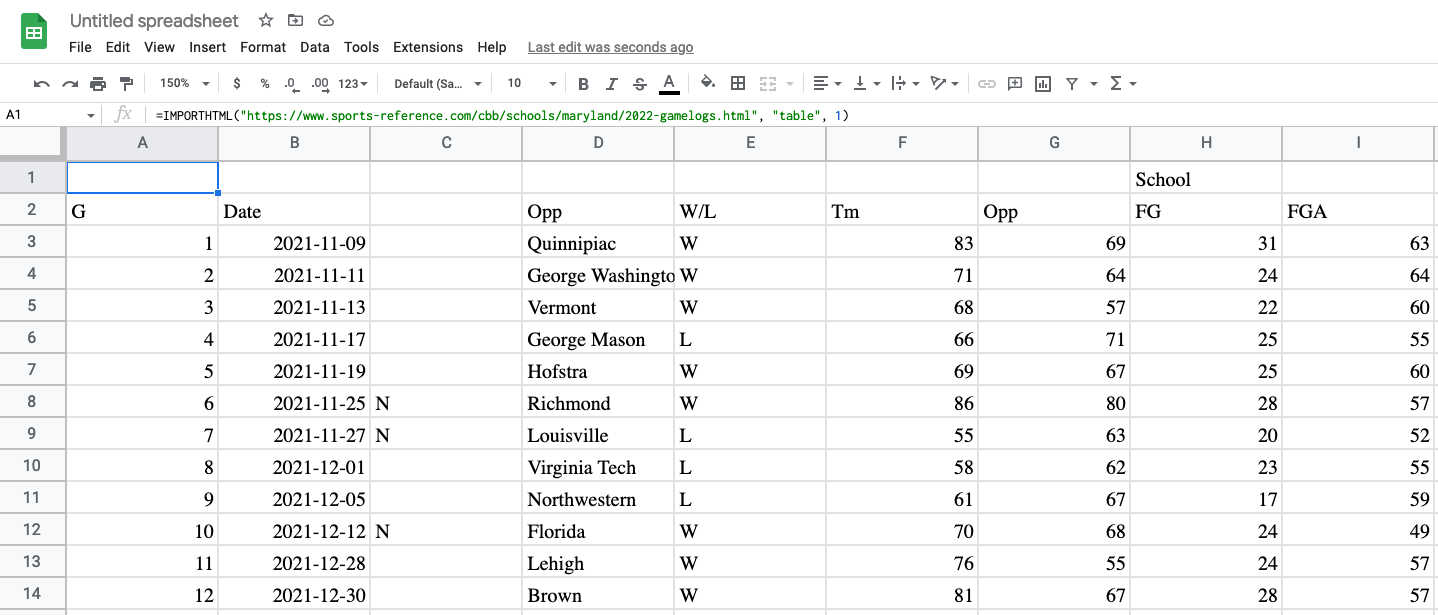
\includegraphics[width=33.28in]{images/clean1}

The solution is easy:

Edit \textgreater{} Select All or type command/control A
Edit \textgreater{} Copy or type command/control c
Edit \textgreater{} Paste Special \textgreater{} Values Only or type command/control shift v

You can verify that it worked by looking in that same row 1 column A, where you'll see the formula is gone.

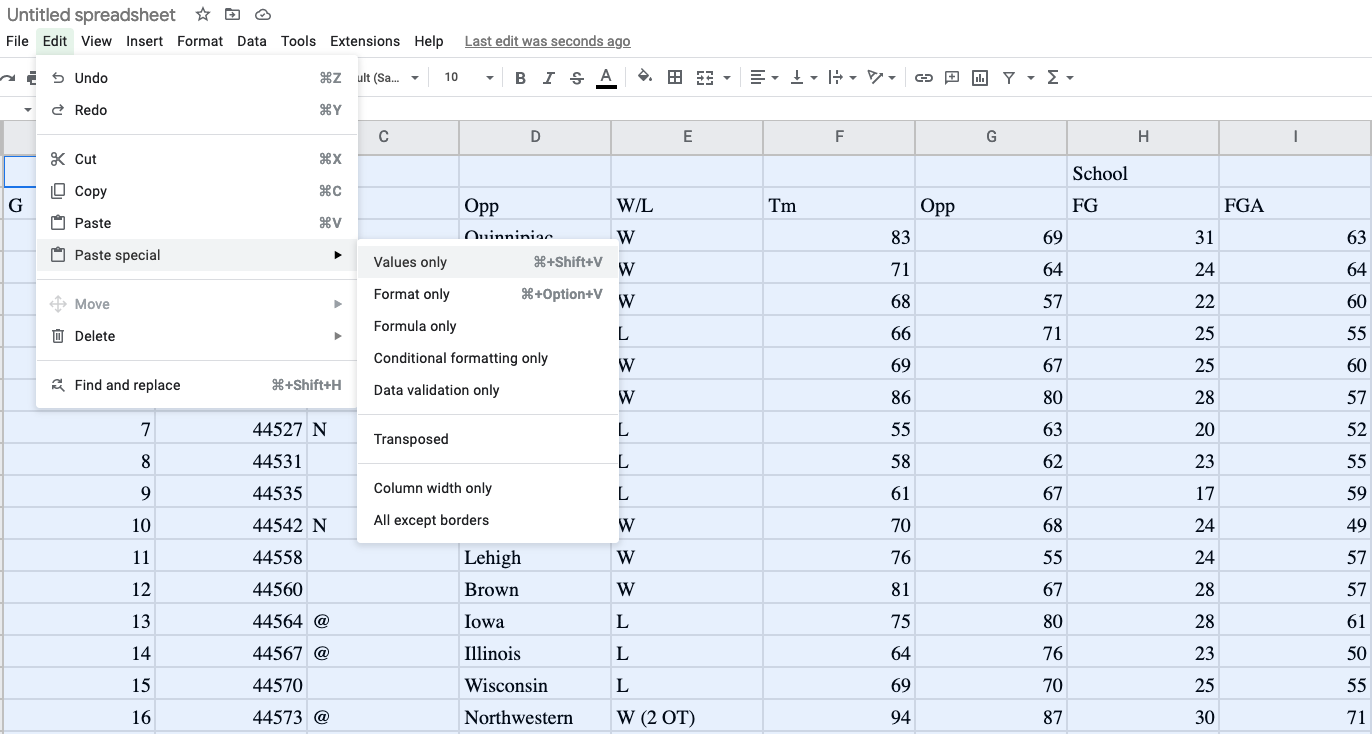
\includegraphics[width=36.81in]{images/clean2}

Now you have data, but your headers are all wrong. You want your headers to be one line -- not two, like they have. And the header names repeat -- first for our team, then for theirs. So you have to change each header name to be UsORB or TeamORB and OpponentORB instead of just ORB.

After you've done that, note we have repeating headers. There's two ways to deal with that -- you could just hightlight it and go up to Edit \textgreater{} Delete Rows XX-XX depending on what rows you highlighted. That's the easy way with our data.

But what if you had hundreds of repeating headers like that? Deleting them would take a long time.

You can use sorting to get rid of anything that's not data. So click on Data \textgreater{} Sort Range. You'll want to check the ``Data has header row'' field. Then hit Sort.

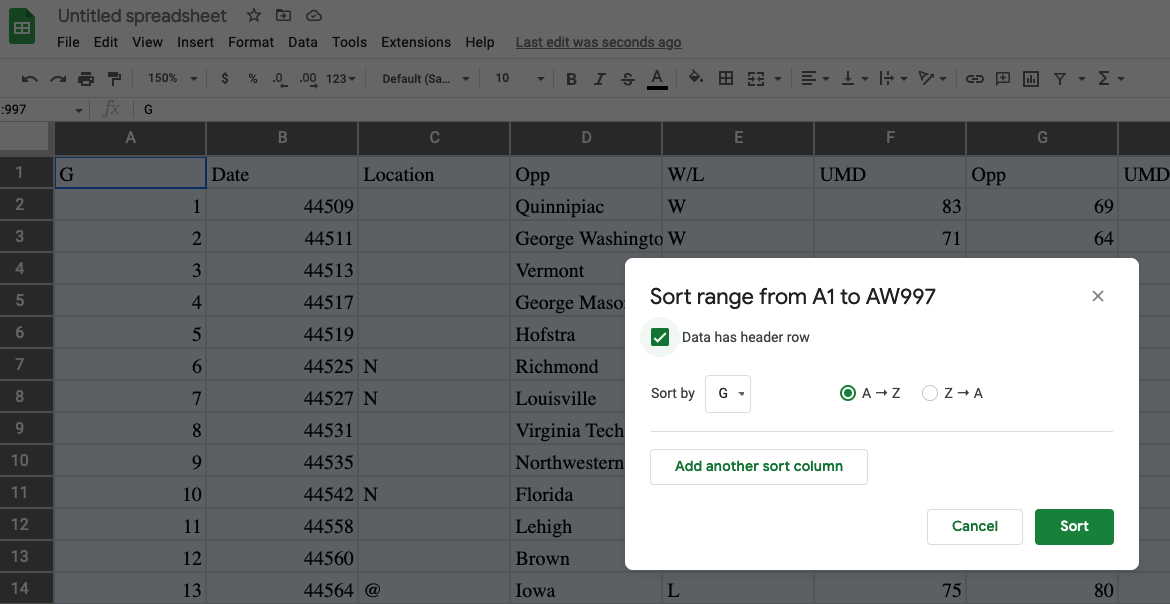
\includegraphics[width=21.61in]{images/clean3}

Now all you need to do is search through the data for where your junk data -- extra headers, blanks, etc. -- got sorted and delete it. After you've done that, you can export it for use in R. Go to File \textgreater{} Download as \textgreater{} Comma Separated Values. Remember to put it in the same directory as your R Notebook file so you can import the data easily.

\hypertarget{aggregates}{%
\chapter{Aggregates}\label{aggregates}}

R is a statistical programming language that is purpose built for data analysis.

Base R does a lot, but there are a mountain of external libraries that do things to make R better/easier/more fully featured. We already installed the tidyverse -- or you should have if you followed the instructions for the last assignment -- which isn't exactly a library, but a collection of libraries. Together, they make up the tidyverse. Individually, they are extraordinarily useful for what they do. We can load them all at once using the tidyverse name, or we can load them individually. Let's start with individually.

The two libraries we are going to need for this assignement are \texttt{readr} and \texttt{dplyr}. The library \texttt{readr} reads different types of data in. For this assignment, we're going to read in csv data or Comma Separated Values data. That's data that has a comma between each column of data.

Then we're going to use \texttt{dplyr} to analyze it.

To use a library, you need to import it. Good practice -- one I'm going to insist on -- is that you put all your library steps at the top of your notebooks.

That code looks like this:

\begin{Shaded}
\begin{Highlighting}[]
\KeywordTok{library}\NormalTok{(readr)}
\end{Highlighting}
\end{Shaded}

To load them both, you need to run that code twice:

\begin{Shaded}
\begin{Highlighting}[]
\KeywordTok{library}\NormalTok{(readr)}
\KeywordTok{library}\NormalTok{(dplyr)}
\end{Highlighting}
\end{Shaded}

You can keep doing that for as many libraries as you need. I've seen notebooks with 10 or more library imports.

\hypertarget{basic-data-analysis-group-by-and-count}{%
\section{Basic data analysis: Group By and Count}\label{basic-data-analysis-group-by-and-count}}

The first thing we need to do is get some data to work with. We do that by reading it in. In our case, we're going to read data from a csv file -- a comma-separated values file.

The CSV file we're going to read from is a \href{https://unl.box.com/s/xjipgkesl9rjmng4weg77vb73xt41apf}{Nebraska Game and Parks Commission dataset} of confirmed mountain lion sightings in Nebraska. There are, on occasion, fierce debates about mountain lions and if they should be hunted in Nebraska. This dataset can tell us some interesting things about that debate.

So step 1 is to import the data. The code looks \emph{something} like this, but hold off copying it just yet:

\texttt{mountainlions\ \textless{}-\ read\_csv("\textasciitilde{}/Documents/Data/mountainlions.csv")}

Let's unpack that.

The first part -- mountainlions -- is the name of your variable. A variable is just a name of a thing. In this case, our variable is a data frame, which is R's way of storing data. We can call this whatever we want. I always want to name data frames after what is in it. In this case, we're going to import a dataset of mountain lion sightings from the Nebraska Game and Parks Commission. Variable names, by convention are one word all lower case. You can end a variable with a number, but you can't start one with a number.

The \textless{}- bit is the variable assignment operator. It's how we know we're assigning something to a word. Think of the arrow as saying ``Take everything on the right of this arrow and stuff it into the thing on the left.'' So we're creating an empty vessel called mountainlions and stuffing all this data into it.

The \texttt{read\_csv} bits are pretty obvious, except for one thing. What happens in the quote marks is the path to the data. In there, I have to tell R where it will find the data. The easiest thing to do, if you are confused about how to find your data, is to put your data in the same folder as as your notebook (you'll have to save that notebook first). If you do that, then you just need to put the name of the file in there (mountainlions.csv). In my case, I've got a folder called Documents in my home directory (that's the \texttt{\textasciitilde{}} part), and in there is a folder called Data that has the file called mountainlions.csv in it. Some people -- insane people -- leave the data in their downloads folder. The data path then would be \texttt{\textasciitilde{}/Downloads/nameofthedatafilehere.csv} on PC or Mac.

\textbf{What you put in there will be different from mine}. So your first task is to import the data.

\begin{Shaded}
\begin{Highlighting}[]
\NormalTok{mountainlions <-}\StringTok{ }\KeywordTok{read_csv}\NormalTok{(}\StringTok{"data/mountainlions.csv"}\NormalTok{)}
\end{Highlighting}
\end{Shaded}

\begin{verbatim}
## Parsed with column specification:
## cols(
##   ID = col_double(),
##   `Cofirm Type` = col_character(),
##   COUNTY = col_character(),
##   Date = col_character()
## )
\end{verbatim}

Now we can inspect the data we imported. What does it look like? To do that, we use \texttt{head(mountainlions)} to show the headers and the first six rows of data. If we wanted to see them all, we could just simply enter \texttt{mountainlions} and run it.

To get the number of records in our dataset, we run \texttt{nrow(mountainlions)}

\begin{Shaded}
\begin{Highlighting}[]
\KeywordTok{head}\NormalTok{(mountainlions)}
\end{Highlighting}
\end{Shaded}

\begin{verbatim}
## # A tibble: 6 x 4
##      ID `Cofirm Type` COUNTY       Date    
##   <dbl> <chr>         <chr>        <chr>   
## 1     1 Track         Dawes        9/14/91 
## 2     2 Mortality     Sioux        11/10/91
## 3     3 Mortality     Scotts Bluff 4/21/96 
## 4     4 Mortality     Sioux        5/9/99  
## 5     5 Mortality     Box Butte    9/29/99 
## 6     6 Track         Scotts Bluff 11/12/99
\end{verbatim}

\begin{Shaded}
\begin{Highlighting}[]
\KeywordTok{nrow}\NormalTok{(mountainlions)}
\end{Highlighting}
\end{Shaded}

\begin{verbatim}
## [1] 393
\end{verbatim}

So what if we wanted to know how many mountain lion sightings there were in each county? To do that by hand, we'd have to take each of the 393 records and sort them into a pile. We'd put them in groups and then count them.

\texttt{dplyr} has a group by function in it that does just this. A massive amount of data analysis involves grouping like things together at some point. So it's a good place to start.

So to do this, we'll take our dataset and we'll introduce a new operator: \%\textgreater{}\%. The best way to read that operator, in my opinion, is to interpret that as ``and then do this.'' Here's the code:

\begin{Shaded}
\begin{Highlighting}[]
\NormalTok{mountainlions }\OperatorTok
\StringTok{  }\KeywordTok{group_by}\NormalTok{(COUNTY) }\OperatorTok
\StringTok{  }\KeywordTok{summarise}\NormalTok{(}
    \DataTypeTok{total =} \KeywordTok{n}\NormalTok{()}
\NormalTok{  )}
\end{Highlighting}
\end{Shaded}

\begin{verbatim}
## # A tibble: 42 x 2
##    COUNTY    total
##    <chr>     <int>
##  1 Banner        6
##  2 Blaine        3
##  3 Box Butte     4
##  4 Brown        15
##  5 Buffalo       3
##  6 Cedar         1
##  7 Cherry       30
##  8 Custer        8
##  9 Dakota        3
## 10 Dawes       111
## # ... with 32 more rows
\end{verbatim}

So let's walk through that. We start with our dataset -- \texttt{mountainlions} -- and then we tell it to group the data by a given field in the data. In this case, we wanted to group together all the counties, signified by the field name COUNTY, which you could get from looking at \texttt{head(mountainlions)}. After we group the data, we need to count them up. In dplyr, we use \texttt{summarize} \href{http://dplyr.tidyverse.org/reference/summarise.html}{which can do more than just count things}. Inside the parentheses in summarize, we set up the summaries we want. In this case, we just want a count of the counties: \texttt{count\ =\ n(),} says create a new field, called \texttt{total} and set it equal to \texttt{n()}, which might look weird, but it's common in stats. The number of things in a dataset? Statisticians call in n. There are n number of incidents in this dataset. So \texttt{n()} is a function that counts the number of things there are.

And when we run that, we get a list of counties with a count next to them. But it's not in any order. So we'll add another And Then Do This \%\textgreater{}\% and use \texttt{arrange}. Arrange does what you think it does -- it arranges data in order. By default, it's in ascending order -- smallest to largest. But if we want to know the county with the most mountain lion sightings, we need to sort it in descending order. That looks like this:

\begin{Shaded}
\begin{Highlighting}[]
\NormalTok{mountainlions }\OperatorTok
\StringTok{  }\KeywordTok{group_by}\NormalTok{(COUNTY) }\OperatorTok
\StringTok{  }\KeywordTok{summarise}\NormalTok{(}
    \DataTypeTok{count =} \KeywordTok{n}\NormalTok{()}
\NormalTok{  ) }\OperatorTok\StringTok{ }\KeywordTok{arrange}\NormalTok{(}\KeywordTok{desc}\NormalTok{(count))}
\end{Highlighting}
\end{Shaded}

\begin{verbatim}
## # A tibble: 42 x 2
##    COUNTY       count
##    <chr>        <int>
##  1 Dawes          111
##  2 Sioux           52
##  3 Sheridan        35
##  4 Cherry          30
##  5 Scotts Bluff    26
##  6 Keya Paha       20
##  7 Brown           15
##  8 Rock            11
##  9 Lincoln         10
## 10 Custer           8
## # ... with 32 more rows
\end{verbatim}

We can, if we want, group by more than one thing. So how are these sightings being confirmed? To do that, we can group by County and ``Cofirm Type'', which is how the state misspelled Confirm. But note something in this example below:

\begin{Shaded}
\begin{Highlighting}[]
\NormalTok{mountainlions }\OperatorTok
\StringTok{  }\KeywordTok{group_by}\NormalTok{(COUNTY, }\StringTok{`}\DataTypeTok{Cofirm Type}\StringTok{`}\NormalTok{) }\OperatorTok
\StringTok{  }\KeywordTok{summarise}\NormalTok{(}
    \DataTypeTok{count =} \KeywordTok{n}\NormalTok{()}
\NormalTok{  ) }\OperatorTok\StringTok{ }\KeywordTok{arrange}\NormalTok{(}\KeywordTok{desc}\NormalTok{(count))}
\end{Highlighting}
\end{Shaded}

\begin{verbatim}
## # A tibble: 93 x 3
## # Groups:   COUNTY [42]
##    COUNTY       `Cofirm Type`      count
##    <chr>        <chr>              <int>
##  1 Dawes        Trail Camera Photo    41
##  2 Sioux        Trail Camera Photo    40
##  3 Dawes        Track                 19
##  4 Keya Paha    Trail Camera Photo    18
##  5 Cherry       Trail Camera Photo    17
##  6 Dawes        Mortality             17
##  7 Sheridan     Trail Camera Photo    16
##  8 Dawes        Photo                 13
##  9 Dawes        DNA                   11
## 10 Scotts Bluff Trail Camera Photo    11
## # ... with 83 more rows
\end{verbatim}

See it? When you have a field name that has two words, \texttt{readr} wraps it in backticks, which is next to the 1 key on your keyboard. You can figure out which fields have backticks around it by looking at the output of \texttt{readr}. Pay attention to that, because it's coming up again in the next section and will be a part of your homework.

\hypertarget{other-aggregates-mean-and-median}{%
\section{Other aggregates: Mean and median}\label{other-aggregates-mean-and-median}}

In the last example, we grouped some data together and counted it up, but there's so much more you can do. You can do multiple measures in a single step as well.

Let's look at some \href{https://unl.box.com/s/09t2u4qoncfh6qlv2156flzlxb8ruzpq}{salary data from the University of Nebraska}.

\begin{Shaded}
\begin{Highlighting}[]
\NormalTok{salaries <-}\StringTok{ }\KeywordTok{read_csv}\NormalTok{(}\StringTok{"data/nusalaries1819.csv"}\NormalTok{)}
\end{Highlighting}
\end{Shaded}

\begin{verbatim}
## Parsed with column specification:
## cols(
##   Employee = col_character(),
##   Position = col_character(),
##   Campus = col_character(),
##   Department = col_character(),
##   `Budgeted Annual Salary` = col_number(),
##   `Salary from State Aided Funds` = col_number(),
##   `Salary from Other Funds` = col_number()
## )
\end{verbatim}

\begin{Shaded}
\begin{Highlighting}[]
\KeywordTok{head}\NormalTok{(salaries)}
\end{Highlighting}
\end{Shaded}

\begin{verbatim}
## # A tibble: 6 x 7
##   Employee Position Campus Department `Budgeted Annua~ `Salary from St~
##   <chr>    <chr>    <chr>  <chr>                 <dbl>            <dbl>
## 1 Abbey, ~ Associa~ UNK    Kinesiolo~            61276            61276
## 2 Abbott,~ Staff S~ UNL    FM&P Faci~            37318               NA
## 3 Abboud,~ Adminis~ UNMC   Surgery-U~            76400            76400
## 4 Abdalla~ Asst Pr~ UNMC   Pathology~            74774            71884
## 5 Abdelka~ Post-Do~ UNMC   Surgery-T~            43516               NA
## 6 Abdel-M~ Researc~ UNL    Public Po~            58502               NA
## # ... with 1 more variable: `Salary from Other Funds` <dbl>
\end{verbatim}

In summarize, we can calculate any number of measures. Here, we'll use R's built in mean and median functions to calculate \ldots{} well, you get the idea.

\begin{Shaded}
\begin{Highlighting}[]
\NormalTok{salaries }\OperatorTok
\StringTok{  }\KeywordTok{summarise}\NormalTok{(}
    \DataTypeTok{count =} \KeywordTok{n}\NormalTok{(),}
    \DataTypeTok{mean_salary =} \KeywordTok{mean}\NormalTok{(}\StringTok{`}\DataTypeTok{Budgeted Annual Salary}\StringTok{`}\NormalTok{),}
    \DataTypeTok{median_salary =} \KeywordTok{median}\NormalTok{(}\StringTok{`}\DataTypeTok{Budgeted Annual Salary}\StringTok{`}\NormalTok{)}
\NormalTok{  )}
\end{Highlighting}
\end{Shaded}

\begin{verbatim}
## # A tibble: 1 x 3
##   count mean_salary median_salary
##   <int>       <dbl>         <dbl>
## 1 13039      62065.         51343
\end{verbatim}

So there's 13,039 employees in the database, spread across four campuses plus the system office. The mean or average salary is about \$62,000, but the median salary is slightly more than \$51,000.

Why?

Let's let sort help us.

\begin{Shaded}
\begin{Highlighting}[]
\NormalTok{salaries }\OperatorTok\StringTok{ }\KeywordTok{arrange}\NormalTok{(}\KeywordTok{desc}\NormalTok{(}\StringTok{`}\DataTypeTok{Budgeted Annual Salary}\StringTok{`}\NormalTok{))}
\end{Highlighting}
\end{Shaded}

\begin{verbatim}
## # A tibble: 13,039 x 7
##    Employee Position Campus Department `Budgeted Annua~ `Salary from St~
##    <chr>    <chr>    <chr>  <chr>                 <dbl>            <dbl>
##  1 Frost, ~ Head Co~ UNL    Athletics           5000000               NA
##  2 Miles, ~ Head Co~ UNL    Athletics           2375000               NA
##  3 Moos, W~ Athleti~ UNL    Athletics           1000000               NA
##  4 Gold, J~ Chancel~ UNMC   Office of~           853338           853338
##  5 Chinand~ Assista~ UNL    Athletics            800000               NA
##  6 Walters~ Assista~ UNL    Athletics            700000               NA
##  7 Cook, J~ Head Co~ UNL    Athletics            675000               NA
##  8 William~ Head Co~ UNL    Athletics            626750               NA
##  9 Bounds,~ Preside~ UNCA   Office of~           540000           540000
## 10 Austin ~ Assista~ UNL    Athletics            475000               NA
## # ... with 13,029 more rows, and 1 more variable: `Salary from Other
## #   Funds` <dbl>
\end{verbatim}

Oh, right. In this dataset, the university pays a football coach \$5 million. Extremes influence averages, not medians, and now you have your answer.

So when choosing a measure of the middle, you have to ask yourself -- could I have extremes? Because a median won't be sensitive to extremes. It will be the point at which half the numbers are above and half are below. The average or mean will be a measure of the middle, but if you have a bunch of low paid people and then one football coach, the average will be wildly skewed. Here, because there's so few highly paid football coaches compared to people who make a normal salary, the number is only slightly skewed in the grand scheme, but skewed nonetheless.

\hypertarget{even-more-aggregates}{%
\section{Even more aggregates}\label{even-more-aggregates}}

There's a ton of things we can do in summarize -- we'll work with more of them as the course progresses -- but here's a few other questions you can ask.

Which department on campus has the highest wage bill? And what is the highest and lowest salary in the department? And how wide is the spread between salaries? We can find that with \texttt{sum} to add up the salaries to get the total wage bill, \texttt{min} to find the minumum salary, \texttt{max} to find the maximum salary and \texttt{sd} to find the standard deviation in the numbers.

\begin{Shaded}
\begin{Highlighting}[]
\NormalTok{salaries }\OperatorTok\StringTok{ }
\StringTok{  }\KeywordTok{group_by}\NormalTok{(Campus, Department) }\OperatorTok\StringTok{ }
\StringTok{  }\KeywordTok{summarise}\NormalTok{(}
    \DataTypeTok{total =} \KeywordTok{sum}\NormalTok{(}\StringTok{`}\DataTypeTok{Budgeted Annual Salary}\StringTok{`}\NormalTok{), }
    \DataTypeTok{avgsalary =} \KeywordTok{mean}\NormalTok{(}\StringTok{`}\DataTypeTok{Budgeted Annual Salary}\StringTok{`}\NormalTok{), }
    \DataTypeTok{minsalary =} \KeywordTok{min}\NormalTok{(}\StringTok{`}\DataTypeTok{Budgeted Annual Salary}\StringTok{`}\NormalTok{),}
    \DataTypeTok{maxsalary =} \KeywordTok{max}\NormalTok{(}\StringTok{`}\DataTypeTok{Budgeted Annual Salary}\StringTok{`}\NormalTok{),}
    \DataTypeTok{stdev =} \KeywordTok{sd}\NormalTok{(}\StringTok{`}\DataTypeTok{Budgeted Annual Salary}\StringTok{`}\NormalTok{)) }\OperatorTok\StringTok{ }\KeywordTok{arrange}\NormalTok{(}\KeywordTok{desc}\NormalTok{(total))}
\end{Highlighting}
\end{Shaded}

\begin{verbatim}
## # A tibble: 804 x 7
## # Groups:   Campus [5]
##    Campus Department                  total avgsalary minsalary maxsalary  stdev
##    <chr>  <chr>                       <dbl>     <dbl>     <dbl>     <dbl>  <dbl>
##  1 UNL    Athletics                  3.56e7   118508.     12925   5000000 3.33e5
##  2 UNMC   Pathology/Microbiology     1.36e7    63158.      1994    186925 3.41e4
##  3 UNL    Agronomy & Horticulture    8.98e6    66496.      5000    208156 4.01e4
##  4 UNMC   Anesthesiology             7.90e6    78237.     10000    245174 3.59e4
##  5 UNL    School of Natural Resour~  6.86e6    65995.      2400    194254 3.28e4
##  6 UNL    College of Law             6.70e6    77953.      1000    326400 7.23e4
##  7 UNL    University Television      6.44e6    55542.     16500    221954 2.75e4
##  8 UNL    University Libraries       6.27e6    51390.      1200    215917 2.68e4
##  9 UNMC   Pharmacology/Exp Neurosc~  6.24e6    58911.      2118    248139 4.29e4
## 10 UNMC   CON-Omaha Division         6.11e6    78304.      3000    172522 4.48e4
## # ... with 794 more rows
\end{verbatim}

So again, no surprise, the UNL athletic department has the single largest wage bill at nearly \$36 million. The average salary in the department is \$118,508 -- more than double the univeristy as a whole, again thanks to Scott Frost's paycheck.

\hypertarget{mutating-data}{%
\chapter{Mutating data}\label{mutating-data}}

One of the most common data analysis techniques is to look at change over time. The most common way of comparing change over time is through percent change. The math behind calculating percent change is very simple, and you should know it off the top of your head. The easy way to remember it is:

\texttt{(new\ -\ old)\ /\ old}

Or new minus old divided by old. Your new number minus the old number, the result of which is divided by the old number. To do that in R, we can use \texttt{dplyr} and \texttt{mutate} to calculate new metrics in a new field using existing fields of data.

So first we'll import the tidyverse so we can read in our data and begin to work with it.

\begin{Shaded}
\begin{Highlighting}[]
\KeywordTok{library}\NormalTok{(tidyverse)}
\end{Highlighting}
\end{Shaded}

Now we'll import a common and \href{https://unl.box.com/s/etqna5bfvf3b0gsnw0kcjjn1rxx9335s}{simple dataset of total attendance} at NCAA football games over the last few seasons.

\begin{Shaded}
\begin{Highlighting}[]
\NormalTok{attendance <-}\StringTok{ }\KeywordTok{read_csv}\NormalTok{(}\StringTok{'data/attendance.csv'}\NormalTok{)}
\end{Highlighting}
\end{Shaded}

\begin{verbatim}
## Parsed with column specification:
## cols(
##   Institution = col_character(),
##   Conference = col_character(),
##   `2013` = col_double(),
##   `2014` = col_double(),
##   `2015` = col_double(),
##   `2016` = col_double(),
##   `2017` = col_double(),
##   `2018` = col_double()
## )
\end{verbatim}

\begin{Shaded}
\begin{Highlighting}[]
\KeywordTok{head}\NormalTok{(attendance)}
\end{Highlighting}
\end{Shaded}

\begin{verbatim}
## # A tibble: 6 x 8
##   Institution     Conference      `2013` `2014` `2015` `2016` `2017` `2018`
##   <chr>           <chr>            <dbl>  <dbl>  <dbl>  <dbl>  <dbl>  <dbl>
## 1 Air Force       MWC             228562 168967 156158 177519 174924 166205
## 2 Akron           MAC             107101  55019 108588  62021 117416  92575
## 3 Alabama         SEC             710538 710736 707786 712747 712053 710931
## 4 Appalachian St. FBS Independent 149366     NA     NA     NA     NA     NA
## 5 Appalachian St. Sun Belt            NA 138995 128755 156916 154722 131716
## 6 Arizona         Pac-12          285713 354973 308355 338017 255791 318051
\end{verbatim}

The code to calculate percent change is pretty simple. Remember, with \texttt{summarize}, we used \texttt{n()} to count things. With \texttt{mutate}, we use very similar syntax to calculate a new value using other values in our dataset. So in this case, we're trying to do (new-old)/old, but we're doing it with fields. If we look at what we got when we did \texttt{head}, you'll see there's `2018` as the new data, and we'll use `2017` as the old data. So we're looking at one year. Then, to help us, we'll use arrange again to sort it, so we get the fastest growing school over one year.

\begin{Shaded}
\begin{Highlighting}[]
\NormalTok{attendance }\OperatorTok\StringTok{ }\KeywordTok{mutate}\NormalTok{(}
  \DataTypeTok{change =}\NormalTok{ (}\StringTok{`}\DataTypeTok{2018}\StringTok{`} \OperatorTok{-}\StringTok{ `}\DataTypeTok{2017}\StringTok{`}\NormalTok{)}\OperatorTok{/}\StringTok{`}\DataTypeTok{2017}\StringTok{`}
\NormalTok{) }
\end{Highlighting}
\end{Shaded}

\begin{verbatim}
## # A tibble: 150 x 9
##    Institution   Conference   `2013` `2014` `2015` `2016` `2017` `2018`   change
##    <chr>         <chr>         <dbl>  <dbl>  <dbl>  <dbl>  <dbl>  <dbl>    <dbl>
##  1 Air Force     MWC          228562 168967 156158 177519 174924 166205 -0.0498 
##  2 Akron         MAC          107101  55019 108588  62021 117416  92575 -0.212  
##  3 Alabama       SEC          710538 710736 707786 712747 712053 710931 -0.00158
##  4 Appalachian ~ FBS Indepen~ 149366     NA     NA     NA     NA     NA NA      
##  5 Appalachian ~ Sun Belt         NA 138995 128755 156916 154722 131716 -0.149  
##  6 Arizona       Pac-12       285713 354973 308355 338017 255791 318051  0.243  
##  7 Arizona St.   Pac-12       501509 343073 368985 286417 359660 291091 -0.191  
##  8 Arkansas      SEC          431174 399124 471279 487067 442569 367748 -0.169  
##  9 Arkansas St.  Sun Belt     149477 149163 138043 136200 119538 119001 -0.00449
## 10 Army West Po~ FBS Indepen~ 169781 171310 185946 163267 185543 190156  0.0249 
## # ... with 140 more rows
\end{verbatim}

What do we see right away? Do those numbers look like we expect them to? No.~They're a decimal expressed as a percentage. So let's fix that by multiplying by 100.

\begin{Shaded}
\begin{Highlighting}[]
\NormalTok{attendance }\OperatorTok\StringTok{ }\KeywordTok{mutate}\NormalTok{(}
  \DataTypeTok{change =}\NormalTok{ ((}\StringTok{`}\DataTypeTok{2018}\StringTok{`} \OperatorTok{-}\StringTok{ `}\DataTypeTok{2017}\StringTok{`}\NormalTok{)}\OperatorTok{/}\StringTok{`}\DataTypeTok{2017}\StringTok{`}\NormalTok{)}\OperatorTok{*}\DecValTok{100}
\NormalTok{) }
\end{Highlighting}
\end{Shaded}

\begin{verbatim}
## # A tibble: 150 x 9
##    Institution    Conference   `2013` `2014` `2015` `2016` `2017` `2018`  change
##    <chr>          <chr>         <dbl>  <dbl>  <dbl>  <dbl>  <dbl>  <dbl>   <dbl>
##  1 Air Force      MWC          228562 168967 156158 177519 174924 166205  -4.98 
##  2 Akron          MAC          107101  55019 108588  62021 117416  92575 -21.2  
##  3 Alabama        SEC          710538 710736 707786 712747 712053 710931  -0.158
##  4 Appalachian S~ FBS Indepen~ 149366     NA     NA     NA     NA     NA  NA    
##  5 Appalachian S~ Sun Belt         NA 138995 128755 156916 154722 131716 -14.9  
##  6 Arizona        Pac-12       285713 354973 308355 338017 255791 318051  24.3  
##  7 Arizona St.    Pac-12       501509 343073 368985 286417 359660 291091 -19.1  
##  8 Arkansas       SEC          431174 399124 471279 487067 442569 367748 -16.9  
##  9 Arkansas St.   Sun Belt     149477 149163 138043 136200 119538 119001  -0.449
## 10 Army West Poi~ FBS Indepen~ 169781 171310 185946 163267 185543 190156   2.49 
## # ... with 140 more rows
\end{verbatim}

Now, does this ordering do anything for us? No.~Let's fix that with arrange.

\begin{Shaded}
\begin{Highlighting}[]
\NormalTok{attendance }\OperatorTok\StringTok{ }\KeywordTok{mutate}\NormalTok{(}
  \DataTypeTok{change =}\NormalTok{ ((}\StringTok{`}\DataTypeTok{2018}\StringTok{`} \OperatorTok{-}\StringTok{ `}\DataTypeTok{2017}\StringTok{`}\NormalTok{)}\OperatorTok{/}\StringTok{`}\DataTypeTok{2017}\StringTok{`}\NormalTok{)}\OperatorTok{*}\DecValTok{100}
\NormalTok{) }\OperatorTok\StringTok{ }\KeywordTok{arrange}\NormalTok{(}\KeywordTok{desc}\NormalTok{(change))}
\end{Highlighting}
\end{Shaded}

\begin{verbatim}
## # A tibble: 150 x 9
##    Institution   Conference `2013` `2014` `2015` `2016` `2017` `2018` change
##    <chr>         <chr>       <dbl>  <dbl>  <dbl>  <dbl>  <dbl>  <dbl>  <dbl>
##  1 Ga. Southern  Sun Belt       NA 105510 124681 104095  61031 100814   65.2
##  2 La.-Monroe    Sun Belt    85177  90540  58659  67057  49640  71048   43.1
##  3 Louisiana     Sun Belt   129878 154652 129577 121346  78754 111303   41.3
##  4 Hawaii        MWC        185931 192159 164031 170299 145463 205455   41.2
##  5 Buffalo       MAC        136418 122418 110743 104957  80102 110280   37.7
##  6 California    Pac-12     345303 286051 292797 279769 219290 300061   36.8
##  7 UCF           AAC        252505 226869 180388 214814 257924 352148   36.5
##  8 UTSA          C-USA      175282 165458 138048 138226 114104 148257   29.9
##  9 Eastern Mich. MAC         20255  75127  29381 106064  73649  95632   29.8
## 10 Louisville    ACC            NA 317829 294413 324391 276957 351755   27.0
## # ... with 140 more rows
\end{verbatim}

So who had the most growth last year from the year before? Something going on at Georgia Southern.

\hypertarget{a-more-complex-example}{%
\section{A more complex example}\label{a-more-complex-example}}

There's metric in basketball that's easy to understand -- shooting percentage. It's the number of shots made divided by the number of shots attempted. Simple, right? Except it's a little too simple. Because what about three point shooters? They tend to be more vailable because the three point shot is worth more. What about players who get to the line? In shooting percentage, free throws are nowhere to be found.

Basketball nerds, because of these weaknesses, have created a new metric called \href{https://en.wikipedia.org/wiki/True_shooting_percentage}{True Shooting Percentage}. True shooting percentage takes into account all aspects of a players shooting to determine who the real shooters are.

Using \texttt{dplyr} and \texttt{mutate}, we can calculate true shooting percentage. So let's look at a new dataset, one of \href{https://unl.box.com/s/s1wzw61u9ia50qmirfhuvprgpmmah9rj}{every college basketball player's season stats in 2018-19 season}. It's a dataset of 5,386 players, and we've got 59 variables -- one of them is True Shooting Percentage, but we're going to ignore that.

\begin{Shaded}
\begin{Highlighting}[]
\NormalTok{players <-}\StringTok{ }\KeywordTok{read_csv}\NormalTok{(}\StringTok{"data/players19.csv"}\NormalTok{)}
\end{Highlighting}
\end{Shaded}

\begin{verbatim}
## Warning: Missing column names filled in: 'X1' [1]
\end{verbatim}

\begin{verbatim}
## Parsed with column specification:
## cols(
##   .default = col_double(),
##   Team = col_character(),
##   Conference = col_character(),
##   Player = col_character(),
##   Class = col_character(),
##   Pos = col_character(),
##   Height = col_character(),
##   Hometown = col_character(),
##   `High School` = col_character(),
##   Summary = col_character()
## )
\end{verbatim}

\begin{verbatim}
## See spec(...) for full column specifications.
\end{verbatim}

The basic true shooting percentage formula is \texttt{(Points\ /\ (2*(FieldGoalAttempts\ +\ (.44\ *\ FreeThrowAttempts))))\ *\ 100}. Let's talk that through. Points divided by a lot. It's really field goal attempts plus 44 percent of the free throw attempts. Why? Because that's about what a free throw is worth, compared to other ways to score. After adding those things together, you double it. And after you divide points by that number, you multiply the whole lot by 100.

In our data, we need to be able to find the fields so we can complete the formula. To do that, one way is to use the Environment tab in R Studio. In the Environment tab is a listing of all the data you've imported, and if you click the triangle next to it, it'll list all the field names, giving you a bit of information about each one.

\includegraphics[width=18.14in]{images/environment}

So what does True Shooting Percentage look like in code?

Let's think about this differently. Who had the best true shooting season last year?

\begin{Shaded}
\begin{Highlighting}[]
\NormalTok{players }\OperatorTok
\StringTok{  }\KeywordTok{mutate}\NormalTok{(}\DataTypeTok{trueshooting =}\NormalTok{ (PTS}\OperatorTok{/}\NormalTok{(}\DecValTok{2}\OperatorTok{*}\NormalTok{(FGA }\OperatorTok{+}\StringTok{ }\NormalTok{(.}\DecValTok{44}\OperatorTok{*}\NormalTok{FTA))))}\OperatorTok{*}\DecValTok{100}\NormalTok{) }\OperatorTok
\StringTok{  }\KeywordTok{arrange}\NormalTok{(}\KeywordTok{desc}\NormalTok{(trueshooting))}
\end{Highlighting}
\end{Shaded}

\begin{verbatim}
## # A tibble: 5,386 x 60
##       X1 Team  Conference Player   `#` Class Pos   Height Weight Hometown
##    <dbl> <chr> <chr>      <chr>  <dbl> <chr> <chr> <chr>   <dbl> <chr>   
##  1   579 Texa~ Big 12     Drayt~     4 JR    G     6-0       156 Austin,~
##  2   843 Ston~ AEC        Nick ~    42 FR    F     6-7       240 Port Je~
##  3  1059 Sout~ Southland  Patri~    22 SO    F     6-3       210 Folsom,~
##  4  4269 Dayt~ A-10       Camro~    52 SO    G     5-7       160 Country~
##  5  4681 Cali~ Pac-12     David~    21 JR    G     6-4       185 Newbury~
##  6   326 Virg~ ACC        Grant~     1 FR    G     <NA>       NA Charlot~
##  7   410 Vand~ SEC        Mac H~    42 FR    G     6-6       182 Chattan~
##  8  1390 Sain~ A-10       Jack ~    31 JR    G     6-6       205 Mattoon~
##  9  2230 NJIT~ A-Sun      Patri~     3 SO    G     5-9       160 West Or~
## 10   266 Wash~ Pac-12     Reaga~    34 FR    F     6-6       225 Santa A~
## # ... with 5,376 more rows, and 50 more variables: `High School` <chr>,
## #   Summary <chr>, Rk.x <dbl>, G <dbl>, GS <dbl>, MP <dbl>, FG <dbl>,
## #   FGA <dbl>, `FG%` <dbl>, `2P` <dbl>, `2PA` <dbl>, `2P%` <dbl>, `3P` <dbl>,
## #   `3PA` <dbl>, `3P%` <dbl>, FT <dbl>, FTA <dbl>, `FT%` <dbl>, ORB <dbl>,
## #   DRB <dbl>, TRB <dbl>, AST <dbl>, STL <dbl>, BLK <dbl>, TOV <dbl>, PF <dbl>,
## #   PTS <dbl>, Rk.y <dbl>, PER <dbl>, `TS%` <dbl>, `eFG%` <dbl>, `3PAr` <dbl>,
## #   FTr <dbl>, PProd <dbl>, `ORB%` <dbl>, `DRB%` <dbl>, `TRB%` <dbl>,
## #   `AST%` <dbl>, `STL%` <dbl>, `BLK%` <dbl>, `TOV%` <dbl>, `USG%` <dbl>,
## #   OWS <dbl>, DWS <dbl>, WS <dbl>, `WS/40` <dbl>, OBPM <dbl>, DBPM <dbl>,
## #   BPM <dbl>, trueshooting <dbl>
\end{verbatim}

You'll be forgiven if you did not hear about Texas Longhorns shooting sensation Drayton Whiteside. He played in six games, took one shot and actually hit it. It happened to be a three pointer, which is one more three pointer than I've hit in college basketball. So props to him. Does that mean he had the best true shooting season in college basketball last year? Not hardly.

We'll talk about how to narrow the pile and filter out data in the next chapter.

\hypertarget{filters-and-selections}{%
\chapter{Filters and selections}\label{filters-and-selections}}

More often than not, we have more data than we want. Sometimes we need to be rid of that data. In \texttt{dplyr}, there's two ways to go about this: filtering and selecting.

\textbf{Filtering creates a subset of the data based on criteria}. All records where the count is greater than 10. All records that match ``Nebraska''. Something like that.

\textbf{Selecting simply returns only the fields named}. So if you only want to see School and Attendance, you select those fields. When you look at your data again, you'll have two columns. If you try to use one of your columns that you had before you used select, you'll get an error.

Let's work with our \href{https://unl.box.com/s/etqna5bfvf3b0gsnw0kcjjn1rxx9335s}{football attendance} data to show some examples.

\begin{Shaded}
\begin{Highlighting}[]
\KeywordTok{library}\NormalTok{(tidyverse)}
\end{Highlighting}
\end{Shaded}

\begin{Shaded}
\begin{Highlighting}[]
\NormalTok{attendance <-}\StringTok{ }\KeywordTok{read_csv}\NormalTok{(}\StringTok{'data/attendance.csv'}\NormalTok{)}
\end{Highlighting}
\end{Shaded}

\begin{verbatim}
## Parsed with column specification:
## cols(
##   Institution = col_character(),
##   Conference = col_character(),
##   `2013` = col_double(),
##   `2014` = col_double(),
##   `2015` = col_double(),
##   `2016` = col_double(),
##   `2017` = col_double(),
##   `2018` = col_double()
## )
\end{verbatim}

So, first things first, let's say we don't care about all this Air Force, Akron, Alabama crap and just want to see Dear Old Nebraska U. We do that with \texttt{filter} and then we pass it a condition.

Before we do that, a note about conditions. Most of the conditional operators you'll understand -- greater than and less than are \textgreater{} and \textless{}. The tough one to remember is equal to. In conditional statements, equal to is == not =. If you haven't noticed, = is a variable assignment operator, not a conditional statement. So equal is == and NOT equal is !=.

So if you want to see Institutions equal to Nebraska, you do this:

\begin{Shaded}
\begin{Highlighting}[]
\NormalTok{attendance }\OperatorTok\StringTok{ }\KeywordTok{filter}\NormalTok{(Institution }\OperatorTok{==}\StringTok{ "Nebraska"}\NormalTok{)}
\end{Highlighting}
\end{Shaded}

\begin{verbatim}
## # A tibble: 1 x 8
##   Institution Conference `2013` `2014` `2015` `2016` `2017` `2018`
##   <chr>       <chr>       <dbl>  <dbl>  <dbl>  <dbl>  <dbl>  <dbl>
## 1 Nebraska    Big Ten    727466 638744 629983 631402 628583 623240
\end{verbatim}

Or if we want to see schools that had more than half a million people buy tickets to a football game in a season, we do the following. NOTE THE BACKTICKS.

\begin{Shaded}
\begin{Highlighting}[]
\NormalTok{attendance }\OperatorTok\StringTok{ }\KeywordTok{filter}\NormalTok{(}\StringTok{`}\DataTypeTok{2018}\StringTok{`} \OperatorTok{>=}\StringTok{ }\DecValTok{500000}\NormalTok{)}
\end{Highlighting}
\end{Shaded}

\begin{verbatim}
## # A tibble: 17 x 8
##    Institution    Conference `2013` `2014` `2015` `2016` `2017` `2018`
##    <chr>          <chr>       <dbl>  <dbl>  <dbl>  <dbl>  <dbl>  <dbl>
##  1 Alabama        SEC        710538 710736 707786 712747 712053 710931
##  2 Auburn         SEC        685252 612157 612157 695498 605120 591236
##  3 Clemson        ACC        574333 572262 588266 566787 565412 562799
##  4 Florida        SEC        524638 515001 630457 439229 520290 576299
##  5 Georgia        SEC        556476 649222 649222 556476 556476 649222
##  6 LSU            SEC        639927 712063 654084 708618 591034 705733
##  7 Michigan       Big Ten    781144 734364 771174 883741 669534 775156
##  8 Michigan St.   Big Ten    506294 522765 522628 522666 507398 508088
##  9 Nebraska       Big Ten    727466 638744 629983 631402 628583 623240
## 10 Ohio St.       Big Ten    734528 744075 750705 750944 752464 713630
## 11 Oklahoma       Big 12     508334 510972 512139 521142 519119 607146
## 12 Penn St.       Big Ten    676112 711358 698590 701800 746946 738396
## 13 South Carolina SEC        576805 569664 472934 538441 550099 515396
## 14 Tennessee      SEC        669087 698276 704088 706776 670454 650887
## 15 Texas          Big 12     593857 564618 540210 587283 556667 586277
## 16 Texas A&M      SEC        697003 630735 725354 713418 691612 698908
## 17 Wisconsin      Big Ten    552378 556642 546099 476144 551766 540072
\end{verbatim}

But what if we want to see all of the Power Five conferences? We \emph{could} use conditional logic in our filter. The conditional logic operators are \texttt{\textbar{}} for OR and \texttt{\&} for AND. NOTE: AND means all conditions have to be met. OR means any of the conditions work. So be careful about boolean logic.

\begin{Shaded}
\begin{Highlighting}[]
\NormalTok{attendance }\OperatorTok\StringTok{ }\KeywordTok{filter}\NormalTok{(Conference }\OperatorTok{==}\StringTok{ "Big 10"} \OperatorTok{|}\StringTok{ }\NormalTok{Conference }\OperatorTok{==}\StringTok{ "SEC"} \OperatorTok{|}\StringTok{ }\NormalTok{Conference }\OperatorTok{==}\StringTok{ "Pac-12"} \OperatorTok{|}\StringTok{ }\NormalTok{Conference }\OperatorTok{==}\StringTok{ "ACC"} \OperatorTok{|}\StringTok{ }\NormalTok{Conference }\OperatorTok{==}\StringTok{ "Big 12"}\NormalTok{)}
\end{Highlighting}
\end{Shaded}

\begin{verbatim}
## # A tibble: 51 x 8
##    Institution    Conference `2013` `2014` `2015` `2016` `2017` `2018`
##    <chr>          <chr>       <dbl>  <dbl>  <dbl>  <dbl>  <dbl>  <dbl>
##  1 Alabama        SEC        710538 710736 707786 712747 712053 710931
##  2 Arizona        Pac-12     285713 354973 308355 338017 255791 318051
##  3 Arizona St.    Pac-12     501509 343073 368985 286417 359660 291091
##  4 Arkansas       SEC        431174 399124 471279 487067 442569 367748
##  5 Auburn         SEC        685252 612157 612157 695498 605120 591236
##  6 Baylor         Big 12     321639 280257 276960 275029 262978 248017
##  7 Boston College ACC        198035 239893 211433 192942 215546 263363
##  8 California     Pac-12     345303 286051 292797 279769 219290 300061
##  9 Clemson        ACC        574333 572262 588266 566787 565412 562799
## 10 Colorado       Pac-12     230778 226670 236331 279652 282335 274852
## # ... with 41 more rows
\end{verbatim}

But that's a lot of repetitive code. And a lot of typing. And typing is the devil. So what if we could create a list and pass it into the filter? It's pretty simple.

We can create a new variable -- remember variables can represent just about anything -- and create a list. To do that we use the \texttt{c} operator, which stands for concatenate. That just means take all the stuff in the parenthesis after the c and bunch it into a list.

Note here: text is in quotes. If they were numbers, we wouldn't need the quotes.

\begin{Shaded}
\begin{Highlighting}[]
\NormalTok{powerfive <-}\StringTok{ }\KeywordTok{c}\NormalTok{(}\StringTok{"SEC"}\NormalTok{, }\StringTok{"Big Ten"}\NormalTok{, }\StringTok{"Pac-12"}\NormalTok{, }\StringTok{"Big 12"}\NormalTok{, }\StringTok{"ACC"}\NormalTok{)}
\end{Highlighting}
\end{Shaded}

Now with a list, we can use the \%in\% operator. It does what you think it does -- it gives you data that matches things IN the list you give it.

\begin{Shaded}
\begin{Highlighting}[]
\NormalTok{attendance }\OperatorTok\StringTok{ }\KeywordTok{filter}\NormalTok{(Conference }\OperatorTok\StringTok{ }\NormalTok{powerfive)}
\end{Highlighting}
\end{Shaded}

\begin{verbatim}
## # A tibble: 65 x 8
##    Institution    Conference `2013` `2014` `2015` `2016` `2017` `2018`
##    <chr>          <chr>       <dbl>  <dbl>  <dbl>  <dbl>  <dbl>  <dbl>
##  1 Alabama        SEC        710538 710736 707786 712747 712053 710931
##  2 Arizona        Pac-12     285713 354973 308355 338017 255791 318051
##  3 Arizona St.    Pac-12     501509 343073 368985 286417 359660 291091
##  4 Arkansas       SEC        431174 399124 471279 487067 442569 367748
##  5 Auburn         SEC        685252 612157 612157 695498 605120 591236
##  6 Baylor         Big 12     321639 280257 276960 275029 262978 248017
##  7 Boston College ACC        198035 239893 211433 192942 215546 263363
##  8 California     Pac-12     345303 286051 292797 279769 219290 300061
##  9 Clemson        ACC        574333 572262 588266 566787 565412 562799
## 10 Colorado       Pac-12     230778 226670 236331 279652 282335 274852
## # ... with 55 more rows
\end{verbatim}

\hypertarget{selecting-data-to-make-it-easier-to-read}{%
\section{Selecting data to make it easier to read}\label{selecting-data-to-make-it-easier-to-read}}

So now we have our Power Five list. What if we just wanted to see attendance from the most recent season and ignore all the rest? Select to the rescue.

\begin{Shaded}
\begin{Highlighting}[]
\NormalTok{attendance }\OperatorTok\StringTok{ }\KeywordTok{filter}\NormalTok{(Conference }\OperatorTok\StringTok{ }\NormalTok{powerfive) }\OperatorTok\StringTok{ }\KeywordTok{select}\NormalTok{(Institution, Conference, }\StringTok{`}\DataTypeTok{2018}\StringTok{`}\NormalTok{)}
\end{Highlighting}
\end{Shaded}

\begin{verbatim}
## # A tibble: 65 x 3
##    Institution    Conference `2018`
##    <chr>          <chr>       <dbl>
##  1 Alabama        SEC        710931
##  2 Arizona        Pac-12     318051
##  3 Arizona St.    Pac-12     291091
##  4 Arkansas       SEC        367748
##  5 Auburn         SEC        591236
##  6 Baylor         Big 12     248017
##  7 Boston College ACC        263363
##  8 California     Pac-12     300061
##  9 Clemson        ACC        562799
## 10 Colorado       Pac-12     274852
## # ... with 55 more rows
\end{verbatim}

If you have truly massive data, Select has tools to help you select fields that start\_with the same things or ends with a certain word. \href{https://dplyr.tidyverse.org/reference/select.html}{The documentation will guide you} if you need those someday. For 90 plus percent of what we do, just naming the fields will be sufficient.

\hypertarget{using-conditional-filters-to-set-limits}{%
\section{Using conditional filters to set limits}\label{using-conditional-filters-to-set-limits}}

Let's return to the blistering season of Drayton Whiteside using our dataset of \href{https://unl.box.com/s/s1wzw61u9ia50qmirfhuvprgpmmah9rj}{every college basketball player's season stats in 2018-19 season}. How can we set limits in something like a question of who had the best season? Let's get our Drayton Whiteside data from the previous chapter back up.

\begin{Shaded}
\begin{Highlighting}[]
\NormalTok{players <-}\StringTok{ }\KeywordTok{read_csv}\NormalTok{(}\StringTok{"data/players19.csv"}\NormalTok{)}
\end{Highlighting}
\end{Shaded}

\begin{verbatim}
## Warning: Missing column names filled in: 'X1' [1]
\end{verbatim}

\begin{verbatim}
## Parsed with column specification:
## cols(
##   .default = col_double(),
##   Team = col_character(),
##   Conference = col_character(),
##   Player = col_character(),
##   Class = col_character(),
##   Pos = col_character(),
##   Height = col_character(),
##   Hometown = col_character(),
##   `High School` = col_character(),
##   Summary = col_character()
## )
\end{verbatim}

\begin{verbatim}
## See spec(...) for full column specifications.
\end{verbatim}

\begin{Shaded}
\begin{Highlighting}[]
\NormalTok{players }\OperatorTok
\StringTok{  }\KeywordTok{mutate}\NormalTok{(}\DataTypeTok{trueshooting =}\NormalTok{ (PTS}\OperatorTok{/}\NormalTok{(}\DecValTok{2}\OperatorTok{*}\NormalTok{(FGA }\OperatorTok{+}\StringTok{ }\NormalTok{(.}\DecValTok{44}\OperatorTok{*}\NormalTok{FTA))))}\OperatorTok{*}\DecValTok{100}\NormalTok{) }\OperatorTok
\StringTok{  }\KeywordTok{arrange}\NormalTok{(}\KeywordTok{desc}\NormalTok{(trueshooting))}
\end{Highlighting}
\end{Shaded}

\begin{verbatim}
## # A tibble: 5,386 x 60
##       X1 Team  Conference Player   `#` Class Pos   Height Weight Hometown
##    <dbl> <chr> <chr>      <chr>  <dbl> <chr> <chr> <chr>   <dbl> <chr>   
##  1   579 Texa~ Big 12     Drayt~     4 JR    G     6-0       156 Austin,~
##  2   843 Ston~ AEC        Nick ~    42 FR    F     6-7       240 Port Je~
##  3  1059 Sout~ Southland  Patri~    22 SO    F     6-3       210 Folsom,~
##  4  4269 Dayt~ A-10       Camro~    52 SO    G     5-7       160 Country~
##  5  4681 Cali~ Pac-12     David~    21 JR    G     6-4       185 Newbury~
##  6   326 Virg~ ACC        Grant~     1 FR    G     <NA>       NA Charlot~
##  7   410 Vand~ SEC        Mac H~    42 FR    G     6-6       182 Chattan~
##  8  1390 Sain~ A-10       Jack ~    31 JR    G     6-6       205 Mattoon~
##  9  2230 NJIT~ A-Sun      Patri~     3 SO    G     5-9       160 West Or~
## 10   266 Wash~ Pac-12     Reaga~    34 FR    F     6-6       225 Santa A~
## # ... with 5,376 more rows, and 50 more variables: `High School` <chr>,
## #   Summary <chr>, Rk.x <dbl>, G <dbl>, GS <dbl>, MP <dbl>, FG <dbl>,
## #   FGA <dbl>, `FG%` <dbl>, `2P` <dbl>, `2PA` <dbl>, `2P%` <dbl>, `3P` <dbl>,
## #   `3PA` <dbl>, `3P%` <dbl>, FT <dbl>, FTA <dbl>, `FT%` <dbl>, ORB <dbl>,
## #   DRB <dbl>, TRB <dbl>, AST <dbl>, STL <dbl>, BLK <dbl>, TOV <dbl>, PF <dbl>,
## #   PTS <dbl>, Rk.y <dbl>, PER <dbl>, `TS%` <dbl>, `eFG%` <dbl>, `3PAr` <dbl>,
## #   FTr <dbl>, PProd <dbl>, `ORB%` <dbl>, `DRB%` <dbl>, `TRB%` <dbl>,
## #   `AST%` <dbl>, `STL%` <dbl>, `BLK%` <dbl>, `TOV%` <dbl>, `USG%` <dbl>,
## #   OWS <dbl>, DWS <dbl>, WS <dbl>, `WS/40` <dbl>, OBPM <dbl>, DBPM <dbl>,
## #   BPM <dbl>, trueshooting <dbl>
\end{verbatim}

In most contests like the batting title in Major League Baseball, there's a minimum number of X to qualify. In baseball, it's at bats. In basketball, it attempts. So let's set a floor and see how it changes. What if we said you had to have played 100 minutes in a season? The top players in college basketball play more than 1000 minutes in a season. So 100 is not that much. Let's try it and see.

\begin{Shaded}
\begin{Highlighting}[]
\NormalTok{players }\OperatorTok
\StringTok{  }\KeywordTok{mutate}\NormalTok{(}\DataTypeTok{trueshooting =}\NormalTok{ (PTS}\OperatorTok{/}\NormalTok{(}\DecValTok{2}\OperatorTok{*}\NormalTok{(FGA }\OperatorTok{+}\StringTok{ }\NormalTok{(.}\DecValTok{44}\OperatorTok{*}\NormalTok{FTA))))}\OperatorTok{*}\DecValTok{100}\NormalTok{) }\OperatorTok
\StringTok{  }\KeywordTok{arrange}\NormalTok{(}\KeywordTok{desc}\NormalTok{(trueshooting)) }\OperatorTok
\StringTok{  }\KeywordTok{filter}\NormalTok{(MP }\OperatorTok{>}\StringTok{ }\DecValTok{100}\NormalTok{)}
\end{Highlighting}
\end{Shaded}

\begin{verbatim}
## # A tibble: 3,659 x 60
##       X1 Team  Conference Player   `#` Class Pos   Height Weight Hometown
##    <dbl> <chr> <chr>      <chr>  <dbl> <chr> <chr> <chr>   <dbl> <chr>   
##  1  4634 Cent~ Southland  Jorda~    33 JR    G     6-1       185 Harriso~
##  2  3623 Hart~ AEC        Max T~    20 SR    G     6-5       200 Rye, NY 
##  3  2675 Mich~ Big Ten    Thoma~    15 FR    F     6-8       225 Clarkst~
##  4  5175 Litt~ Sun Belt   Kris ~    32 SO    F     6-8       194 Dewitt,~
##  5  5205 Ariz~ Pac-12     De'Qu~    32 SR    F     6-10      225 St. Tho~
##  6  4099 ETSU~ Southern   Lucas~    25 JR    C     7-0       220 De Lier~
##  7  3006 Loui~ Sun Belt   Brand~     0 SR    G     6-4       180 Hawthor~
##  8   570 Texa~ Big 12     Jaxso~    10 FR    F     6-11      220 Lovelan~
##  9  1704 Pepp~ WCC        Victo~    34 FR    C     6-9       200 Owerri,~
## 10  4056 East~ MAC        Jalen~    30 SO    F     6-9       215 Pasco, ~
## # ... with 3,649 more rows, and 50 more variables: `High School` <chr>,
## #   Summary <chr>, Rk.x <dbl>, G <dbl>, GS <dbl>, MP <dbl>, FG <dbl>,
## #   FGA <dbl>, `FG%` <dbl>, `2P` <dbl>, `2PA` <dbl>, `2P%` <dbl>, `3P` <dbl>,
## #   `3PA` <dbl>, `3P%` <dbl>, FT <dbl>, FTA <dbl>, `FT%` <dbl>, ORB <dbl>,
## #   DRB <dbl>, TRB <dbl>, AST <dbl>, STL <dbl>, BLK <dbl>, TOV <dbl>, PF <dbl>,
## #   PTS <dbl>, Rk.y <dbl>, PER <dbl>, `TS%` <dbl>, `eFG%` <dbl>, `3PAr` <dbl>,
## #   FTr <dbl>, PProd <dbl>, `ORB%` <dbl>, `DRB%` <dbl>, `TRB%` <dbl>,
## #   `AST%` <dbl>, `STL%` <dbl>, `BLK%` <dbl>, `TOV%` <dbl>, `USG%` <dbl>,
## #   OWS <dbl>, DWS <dbl>, WS <dbl>, `WS/40` <dbl>, OBPM <dbl>, DBPM <dbl>,
## #   BPM <dbl>, trueshooting <dbl>
\end{verbatim}

Now you get Central Arkansas Bears Junior Jordan Grant, who played in 25 games and was on the floor for 152 minutes. So he played regularly. But in that time, he only attempted 16 shots, and made 68 percent of them. In other words, when he shot, he probably scored. He just rarely shot.

So is 100 minutes our level? Here's the truth -- there's not really an answer here. We're picking a cutoff. If you can cite a reason for it and defend it, then it probably works.

\hypertarget{top-list}{%
\section{Top list}\label{top-list}}

One last little dplyr trick that's nice to have in the toolbox is a shortcut for selecting only the top values for your dataset. Want to make a Top 10 List? Or Top 25? Or Top Whatever You Want? It's easy.

So what are the top 10 Power Five schools by season attendance. All we're doing here is chaining commands together with what we've already got. We're \emph{filtering} by our list of Power Five conferences, we're \emph{selecting} the three fields we need, now we're going to \emph{arrange} it by total attendance and then we'll introduce the new function: \texttt{top\_n}. The \texttt{top\_n} function just takes a number. So we want a top 10 list? We do it like this:

\begin{Shaded}
\begin{Highlighting}[]
\NormalTok{attendance }\OperatorTok\StringTok{ }\KeywordTok{filter}\NormalTok{(Conference }\OperatorTok\StringTok{ }\NormalTok{powerfive) }\OperatorTok\StringTok{ }\KeywordTok{select}\NormalTok{(Institution, Conference, }\StringTok{`}\DataTypeTok{2018}\StringTok{`}\NormalTok{) }\OperatorTok\StringTok{ }\KeywordTok{arrange}\NormalTok{(}\KeywordTok{desc}\NormalTok{(}\StringTok{`}\DataTypeTok{2018}\StringTok{`}\NormalTok{)) }\OperatorTok\StringTok{ }\KeywordTok{top_n}\NormalTok{(}\DecValTok{10}\NormalTok{)}
\end{Highlighting}
\end{Shaded}

\begin{verbatim}
## Selecting by 2018
\end{verbatim}

\begin{verbatim}
## # A tibble: 10 x 3
##    Institution Conference `2018`
##    <chr>       <chr>       <dbl>
##  1 Michigan    Big Ten    775156
##  2 Penn St.    Big Ten    738396
##  3 Ohio St.    Big Ten    713630
##  4 Alabama     SEC        710931
##  5 LSU         SEC        705733
##  6 Texas A&M   SEC        698908
##  7 Tennessee   SEC        650887
##  8 Georgia     SEC        649222
##  9 Nebraska    Big Ten    623240
## 10 Oklahoma    Big 12     607146
\end{verbatim}

That's all there is to it. Just remember -- for it to work correctly, you need to sort your data BEFORE you run top\_n. Otherwise, you're just getting the first 10 values in the list. The function doesn't know what field you want the top values of. You have to do it.

\hypertarget{transforming-data}{%
\chapter{Transforming data}\label{transforming-data}}

Sometimes long data needs to be wide, and sometimes wide data needs to be long. I'll explain.

You are soon going to discover that long before you can visualize data, \textbf{you need to have it in a form that the visualization library can deal with}. One of the ways that isn't immediately obvious is \textbf{how your data is cast}. Most of the data you will encounter will be \textbf{wide -- each row will represent a single entity with multiple measures for that entity}. So think of states. Your row of your dataset could have the state name, population, average life expectancy and other demographic data.

But what if your visualization library needs one row for each measure? So state, data type and the data. Nebraska, Population, 1,929,000. That's one row. Then the next row is Nebraska, Average Life Expectancy, 76. That's the next row. That's where recasting your data comes in.

We can use a library called \texttt{tidyr} to \texttt{pivot\_longer} or \texttt{pivot\_wider} the data, depending on what we need. We'll use a \href{https://unl.box.com/s/etqna5bfvf3b0gsnw0kcjjn1rxx9335s}{dataset of college football attendance} to demonstrate. First we need some libraries.

\begin{Shaded}
\begin{Highlighting}[]
\KeywordTok{library}\NormalTok{(tidyverse)}
\end{Highlighting}
\end{Shaded}

Now we'll load the data.

\begin{Shaded}
\begin{Highlighting}[]
\NormalTok{attendance <-}\StringTok{ }\KeywordTok{read_csv}\NormalTok{(}\StringTok{'data/attendance.csv'}\NormalTok{)}
\end{Highlighting}
\end{Shaded}

\begin{verbatim}
## Parsed with column specification:
## cols(
##   Institution = col_character(),
##   Conference = col_character(),
##   `2013` = col_double(),
##   `2014` = col_double(),
##   `2015` = col_double(),
##   `2016` = col_double(),
##   `2017` = col_double(),
##   `2018` = col_double()
## )
\end{verbatim}

\begin{Shaded}
\begin{Highlighting}[]
\NormalTok{attendance}
\end{Highlighting}
\end{Shaded}

\begin{verbatim}
## # A tibble: 150 x 8
##    Institution     Conference      `2013` `2014` `2015` `2016` `2017` `2018`
##    <chr>           <chr>            <dbl>  <dbl>  <dbl>  <dbl>  <dbl>  <dbl>
##  1 Air Force       MWC             228562 168967 156158 177519 174924 166205
##  2 Akron           MAC             107101  55019 108588  62021 117416  92575
##  3 Alabama         SEC             710538 710736 707786 712747 712053 710931
##  4 Appalachian St. FBS Independent 149366     NA     NA     NA     NA     NA
##  5 Appalachian St. Sun Belt            NA 138995 128755 156916 154722 131716
##  6 Arizona         Pac-12          285713 354973 308355 338017 255791 318051
##  7 Arizona St.     Pac-12          501509 343073 368985 286417 359660 291091
##  8 Arkansas        SEC             431174 399124 471279 487067 442569 367748
##  9 Arkansas St.    Sun Belt        149477 149163 138043 136200 119538 119001
## 10 Army West Point FBS Independent 169781 171310 185946 163267 185543 190156
## # ... with 140 more rows
\end{verbatim}

So as you can see, each row represents a school, and then each column represents a year. This is great for calculating the percent change -- we can subtract a column from a column and divide by that column. But later, when we want to chart each school's attendance over the years, we have to have each row be one team for one year. Nebraska in 2013, then Nebraska in 2014, and Nebraska in 2015 and so on.

To do that, we use \texttt{pivot\_longer} because we're making wide data long. Since all of the columns we want to make rows start with 20, we can use that in our \texttt{cols} directive. Then we give that column a name -- Year -- and the values for each year need a name too. Those are the attendance figure. We can see right away how this works.

\begin{Shaded}
\begin{Highlighting}[]
\NormalTok{attendance }\OperatorTok\StringTok{ }\KeywordTok{pivot_longer}\NormalTok{(}\DataTypeTok{cols =} \KeywordTok{starts_with}\NormalTok{(}\StringTok{"20"}\NormalTok{), }\DataTypeTok{names_to =} \StringTok{"Year"}\NormalTok{, }\DataTypeTok{values_to =} \StringTok{"Attendance"}\NormalTok{)}
\end{Highlighting}
\end{Shaded}

\begin{verbatim}
## # A tibble: 900 x 4
##    Institution Conference Year  Attendance
##    <chr>       <chr>      <chr>      <dbl>
##  1 Air Force   MWC        2013      228562
##  2 Air Force   MWC        2014      168967
##  3 Air Force   MWC        2015      156158
##  4 Air Force   MWC        2016      177519
##  5 Air Force   MWC        2017      174924
##  6 Air Force   MWC        2018      166205
##  7 Akron       MAC        2013      107101
##  8 Akron       MAC        2014       55019
##  9 Akron       MAC        2015      108588
## 10 Akron       MAC        2016       62021
## # ... with 890 more rows
\end{verbatim}

We've gone from 150 rows to 900, but that's expected when we have 6 years for each team.

\hypertarget{making-long-data-wide}{%
\section{Making long data wide}\label{making-long-data-wide}}

We can reverse this process using \texttt{pivot\_wider}, which makes long data wide.

Why do any of this?

In some cases, you're going to be given long data and you need to calculate some metric using two of the years -- a percent change for instance. So you'll need to make the data wide to do that. You might then have to re-lengthen the data now with the percent change. Some project require you to do all kinds of flexing like this. It just depends on the data.

So let's take what we made above and turn it back into wide data.

\begin{Shaded}
\begin{Highlighting}[]
\NormalTok{longdata <-}\StringTok{ }\NormalTok{attendance }\OperatorTok\StringTok{ }\KeywordTok{pivot_longer}\NormalTok{(}\DataTypeTok{cols =} \KeywordTok{starts_with}\NormalTok{(}\StringTok{"20"}\NormalTok{), }\DataTypeTok{names_to =} \StringTok{"Year"}\NormalTok{, }\DataTypeTok{values_to =} \StringTok{"Attendance"}\NormalTok{)}

\NormalTok{longdata}
\end{Highlighting}
\end{Shaded}

\begin{verbatim}
## # A tibble: 900 x 4
##    Institution Conference Year  Attendance
##    <chr>       <chr>      <chr>      <dbl>
##  1 Air Force   MWC        2013      228562
##  2 Air Force   MWC        2014      168967
##  3 Air Force   MWC        2015      156158
##  4 Air Force   MWC        2016      177519
##  5 Air Force   MWC        2017      174924
##  6 Air Force   MWC        2018      166205
##  7 Akron       MAC        2013      107101
##  8 Akron       MAC        2014       55019
##  9 Akron       MAC        2015      108588
## 10 Akron       MAC        2016       62021
## # ... with 890 more rows
\end{verbatim}

To \texttt{pivot\_wider}, we just need to say where our column names are coming from -- the Year -- and where the data under it should come from -- Attendance.

\begin{Shaded}
\begin{Highlighting}[]
\NormalTok{longdata }\OperatorTok\StringTok{ }\KeywordTok{pivot_wider}\NormalTok{(}\DataTypeTok{names_from =}\NormalTok{ Year, }\DataTypeTok{values_from =}\NormalTok{ Attendance)}
\end{Highlighting}
\end{Shaded}

\begin{verbatim}
## # A tibble: 150 x 8
##    Institution     Conference      `2013` `2014` `2015` `2016` `2017` `2018`
##    <chr>           <chr>            <dbl>  <dbl>  <dbl>  <dbl>  <dbl>  <dbl>
##  1 Air Force       MWC             228562 168967 156158 177519 174924 166205
##  2 Akron           MAC             107101  55019 108588  62021 117416  92575
##  3 Alabama         SEC             710538 710736 707786 712747 712053 710931
##  4 Appalachian St. FBS Independent 149366     NA     NA     NA     NA     NA
##  5 Appalachian St. Sun Belt            NA 138995 128755 156916 154722 131716
##  6 Arizona         Pac-12          285713 354973 308355 338017 255791 318051
##  7 Arizona St.     Pac-12          501509 343073 368985 286417 359660 291091
##  8 Arkansas        SEC             431174 399124 471279 487067 442569 367748
##  9 Arkansas St.    Sun Belt        149477 149163 138043 136200 119538 119001
## 10 Army West Point FBS Independent 169781 171310 185946 163267 185543 190156
## # ... with 140 more rows
\end{verbatim}

And just like that, we're back.

\hypertarget{why-this-matters}{%
\section{Why this matters}\label{why-this-matters}}

This matters because certain visualization types need wide or long data. A significant hurdle you will face for the rest of the semester is getting the data in the right format for what you want to do.

So let me walk you through an example using this data.

Let's look at Nebraska's attendance over the time period. In order to do that, I need long data because that's what the charting library, \texttt{ggplot2}, needs. You're going to learn a lot more about ggplot later.

\begin{Shaded}
\begin{Highlighting}[]
\NormalTok{nebraska <-}\StringTok{ }\NormalTok{longdata }\OperatorTok\StringTok{ }\KeywordTok{filter}\NormalTok{(Institution }\OperatorTok{==}\StringTok{ "Nebraska"}\NormalTok{)}
\end{Highlighting}
\end{Shaded}

Now that we have long data for just Nebraska, we can chart it.

\begin{Shaded}
\begin{Highlighting}[]
\KeywordTok{ggplot}\NormalTok{(nebraska, }\KeywordTok{aes}\NormalTok{(}\DataTypeTok{x=}\NormalTok{Year, }\DataTypeTok{y=}\NormalTok{Attendance, }\DataTypeTok{group=}\DecValTok{1}\NormalTok{)) }\OperatorTok{+}\StringTok{ }
\StringTok{  }\KeywordTok{geom_line}\NormalTok{() }\OperatorTok{+}\StringTok{ }
\StringTok{  }\KeywordTok{scale_y_continuous}\NormalTok{(}\DataTypeTok{labels =}\NormalTok{ scales}\OperatorTok{::}\NormalTok{comma) }\OperatorTok{+}\StringTok{ }
\StringTok{  }\KeywordTok{labs}\NormalTok{(}\DataTypeTok{x=}\StringTok{"Year"}\NormalTok{, }\DataTypeTok{y=}\StringTok{"Attendance"}\NormalTok{, }\DataTypeTok{title=}\StringTok{"We'll all stick together?"}\NormalTok{, }\DataTypeTok{subtitle=}\StringTok{"It's not as bad as you think -- they widened the seats, cutting the number."}\NormalTok{, }\DataTypeTok{caption=}\StringTok{"Source: NCAA | By Matt Waite"}\NormalTok{, }\DataTypeTok{color =} \StringTok{"Outcome"}\NormalTok{) }\OperatorTok{+}
\StringTok{  }\KeywordTok{theme_minimal}\NormalTok{() }\OperatorTok{+}\StringTok{ }
\StringTok{  }\KeywordTok{theme}\NormalTok{(}
    \DataTypeTok{plot.title =} \KeywordTok{element_text}\NormalTok{(}\DataTypeTok{size =} \DecValTok{16}\NormalTok{, }\DataTypeTok{face =} \StringTok{"bold"}\NormalTok{),}
    \DataTypeTok{axis.title =} \KeywordTok{element_text}\NormalTok{(}\DataTypeTok{size =} \DecValTok{10}\NormalTok{),}
    \DataTypeTok{axis.title.y =} \KeywordTok{element_blank}\NormalTok{(),}
    \DataTypeTok{axis.text =} \KeywordTok{element_text}\NormalTok{(}\DataTypeTok{size =} \DecValTok{7}\NormalTok{),}
    \DataTypeTok{axis.ticks =} \KeywordTok{element_blank}\NormalTok{(),}
    \DataTypeTok{panel.grid.minor =} \KeywordTok{element_blank}\NormalTok{(),}
    \DataTypeTok{panel.grid.major.x =} \KeywordTok{element_blank}\NormalTok{(),}
    \DataTypeTok{legend.position=}\StringTok{"bottom"}
\NormalTok{  )}
\end{Highlighting}
\end{Shaded}

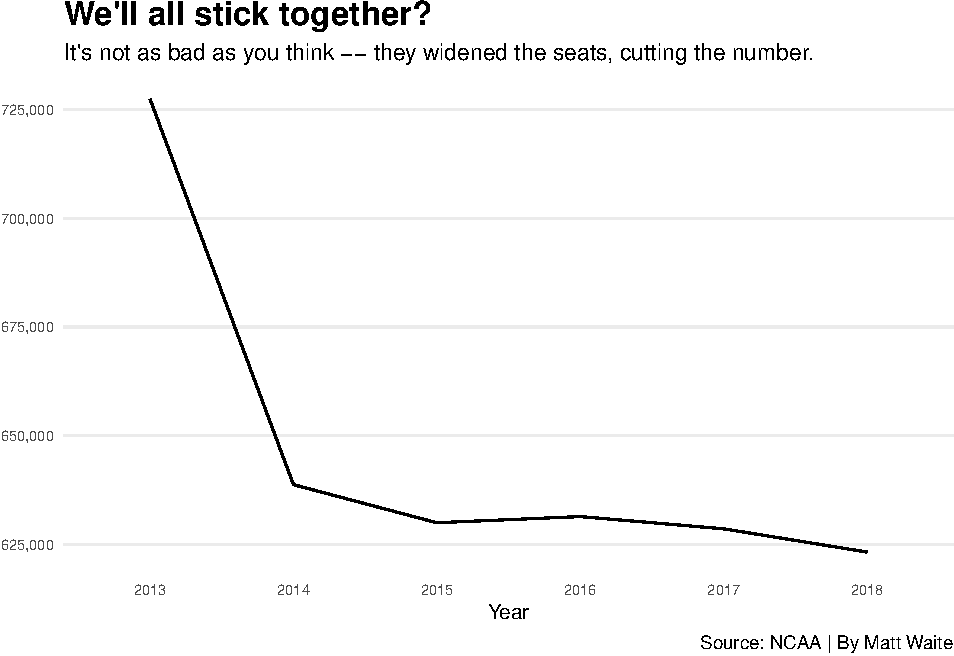
\includegraphics{SportsData_files/figure-latex/unnamed-chunk-49-1.pdf}

\hypertarget{simulations}{%
\chapter{Simulations}\label{simulations}}

Two seasons ago, James Palmer Jr.~shot 139 three point attempts and made 43 of them for a .309 shooting percentage last year. A few weeks into last season, he was 7 for 39 -- a paltry .179. Is something wrong or is this just bad luck?

Luck is something that comes up a lot in sports. Is a team unlucky? Or a player? One way we can get to this, we can get to that is by simulating things based on their typical percentages. Simulations work by choosing random values within a range based on a distribution. The most common distribution is the normal or binomial distribution. The normal distribution is where the most cases appear around the mean, 66 percent of cases are within one standard deviation from the mean, and the further away from the mean you get, the more rare things become.

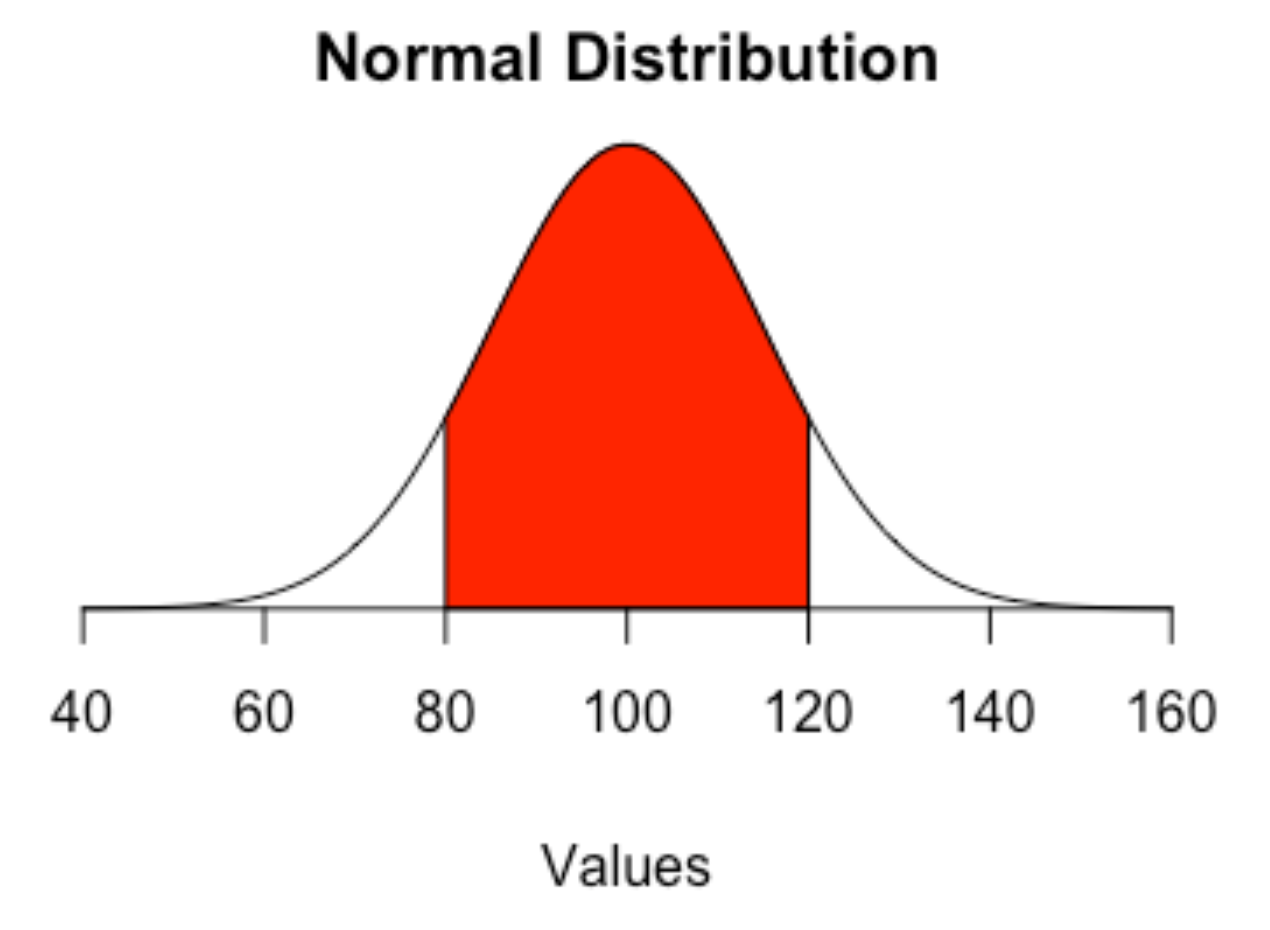
\includegraphics[width=17.64in]{images/simulations2}

Let's simulate 39 three point attempts 1000 times with his season long shooting percentage and see if this could just be random chance or something else.

We do this using a base R function called \texttt{rbinom} or binomial distribution. So what that means is there's a normally distrubuted chance that James Palmer Jr.~is going to shoot above and below his career three point shooting percentage. If we randomly assign values in that distribution 1000 times, how many times will it come up 7, like this example?

\begin{Shaded}
\begin{Highlighting}[]
\KeywordTok{set.seed}\NormalTok{(}\DecValTok{1234}\NormalTok{)}

\NormalTok{simulations <-}\StringTok{ }\KeywordTok{rbinom}\NormalTok{(}\DataTypeTok{n =} \DecValTok{1000}\NormalTok{, }\DataTypeTok{size =} \DecValTok{39}\NormalTok{, }\DataTypeTok{prob =} \FloatTok{.309}\NormalTok{)}

\KeywordTok{table}\NormalTok{(simulations)}
\end{Highlighting}
\end{Shaded}

\begin{verbatim}
## simulations
##   3   4   5   6   7   8   9  10  11  12  13  14  15  16  17  18  19  20  21  22 
##   1   4   5  12  35  44  76 117 134 135 135  99  71  53  37  21  15   2   3   1
\end{verbatim}

How do we read this? The first row and the second row form a pair. The top row is the number of shots made. The number immediately under it is the number of simulations where that occurred.

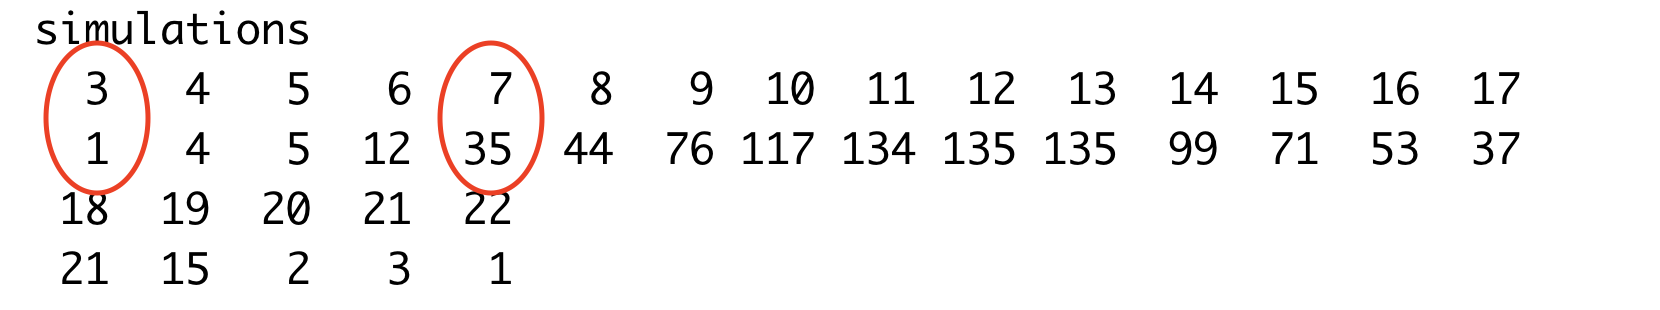
\includegraphics[width=23.06in]{images/simulations1}

So what we see is given his season long shooting percentage, it's not out of the realm of randomness that with just 39 attempts for Palmer, he's only hit only 7. In 1000 simulations, it comes up 35 times. Is he below where he should be? Yes. Will he likely improve and soon? Unless something is very wrong, yes. And indeed, by the end of the season, he finished with a .313 shooting percentage from 3 point range. So we can say he was just unlucky.

\hypertarget{cold-streaks}{%
\section{Cold streaks}\label{cold-streaks}}

During the Western Illinois game, the team, shooting .329 on the season from behind the arc, went 0-15 in the second half. How strange is that?

\begin{Shaded}
\begin{Highlighting}[]
\KeywordTok{set.seed}\NormalTok{(}\DecValTok{1234}\NormalTok{)}

\NormalTok{simulations <-}\StringTok{ }\KeywordTok{rbinom}\NormalTok{(}\DataTypeTok{n =} \DecValTok{1000}\NormalTok{, }\DataTypeTok{size =} \DecValTok{15}\NormalTok{, }\DataTypeTok{prob =} \FloatTok{.329}\NormalTok{)}

\KeywordTok{hist}\NormalTok{(simulations)}
\end{Highlighting}
\end{Shaded}

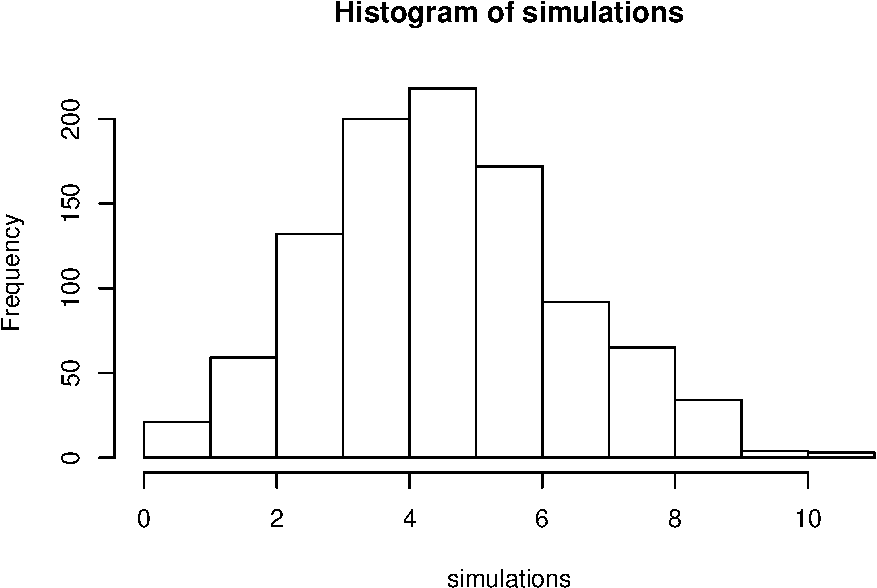
\includegraphics{SportsData_files/figure-latex/unnamed-chunk-53-1.pdf}

\begin{Shaded}
\begin{Highlighting}[]
\KeywordTok{table}\NormalTok{(simulations)}
\end{Highlighting}
\end{Shaded}

\begin{verbatim}
## simulations
##   0   1   2   3   4   5   6   7   8   9  10  11 
##   5  16  59 132 200 218 172  92  65  34   4   3
\end{verbatim}

Short answer: Really weird. If you simulate 15 threes 1000 times, sometimes you'll see them miss all of them, but only a few times -- five times, in this case. Most of the time, the team won't go 0-15 even once. So going ice cold is not totally out of the realm of random chance, but it's highly unlikely.

\hypertarget{correlations-and-regression}{%
\chapter{Correlations and regression}\label{correlations-and-regression}}

Throughout sports, you will find no shortage of opinions. From people yelling at their TV screens to an entire industry of people paid to have opinions, there are no shortage of reasons why this team sucks and that player is great. They may have their reasons, but a better question is, does that reason really matter?

Can we put some numbers behind that? Can we prove it or not?

This is what we're going to start to answer. And we'll do it with correlations and regressions.

First, we need libraries and \href{https://unl.box.com/s/zlxoptqixkt98gubk3i6316qun99l49r}{data}.

\begin{Shaded}
\begin{Highlighting}[]
\KeywordTok{library}\NormalTok{(tidyverse)}
\end{Highlighting}
\end{Shaded}

\begin{Shaded}
\begin{Highlighting}[]
\NormalTok{correlations <-}\StringTok{ }\KeywordTok{read_csv}\NormalTok{(}\StringTok{"data/correlations.csv"}\NormalTok{)}
\end{Highlighting}
\end{Shaded}

\begin{verbatim}
## Parsed with column specification:
## cols(
##   Name = col_character(),
##   OffPoints = col_double(),
##   OffPointsG = col_double(),
##   DefPoints = col_double(),
##   DefPointsG = col_double(),
##   Pen. = col_double(),
##   Yards = col_double(),
##   `Pen./G` = col_double(),
##   OffConversions = col_double(),
##   OffConversionPct = col_double(),
##   DefConversions = col_double(),
##   DefConversionPct = col_double()
## )
\end{verbatim}

To do this, we need all FBS college football teams and their season stats from last year. How much, over the course of a season, does a thing matter? That's the question you're going to answer.

In our case, we want to know how much does a team's accumulated penalties influence the number of points they score in a season? How much difference can we explain in points with penalties?

We're going to use two different methods here and they're closely related. Correlations -- specifically the Pearson Correlation Coefficient -- is a measure of how related two numbers are in a linear fashion. In other words -- if our X value goes up one, what happens to Y? If it also goes up 1, that's a perfect correlation. X goes up 1, Y goes up 1. Every time. Correlation coefficients are a number between 0 and 1, with zero being no correlation and 1 being perfect correlation \textbf{if our data is linear}. We'll soon go over scatterplots to visually determine if our data is linear, but for now, we have a hypothesis: More penalties are bad. Penalties hurt. So if a team gets lots of them, they should have worse outcomes than teams that get few of them. That is an argument for a linear relationship between them.

But is there one?

We're going create a new dataframe called newcorrelations that takes our data that we imported and adds a column called \texttt{differential} because we don't have separate offense and defense penalties, and then we'll use correlations to see how related those two things are.

\begin{Shaded}
\begin{Highlighting}[]
\NormalTok{newcorrelations <-}\StringTok{ }\NormalTok{correlations }\OperatorTok\StringTok{ }
\StringTok{  }\KeywordTok{mutate}\NormalTok{(}\DataTypeTok{differential =}\NormalTok{ OffPoints }\OperatorTok{-}\StringTok{ }\NormalTok{DefPoints)}
\end{Highlighting}
\end{Shaded}

In R, there is a \texttt{cor} function, and it works much the same as \texttt{mean} or \texttt{median}. So we want to see if \texttt{differential} is correlated with \texttt{Yards}, which is the yards of penalties a team gets in a game. We do that by referenceing \texttt{differential} and \texttt{Yards} and specifying we want a \texttt{pearson} correlation. The number we get back is the correlation coefficient.

\begin{Shaded}
\begin{Highlighting}[]
\NormalTok{newcorrelations }\OperatorTok\StringTok{ }\KeywordTok{summarise}\NormalTok{(}\DataTypeTok{correlation =} \KeywordTok{cor}\NormalTok{(differential, Yards, }\DataTypeTok{method=}\StringTok{"pearson"}\NormalTok{))}
\end{Highlighting}
\end{Shaded}

\begin{verbatim}
## # A tibble: 1 x 1
##   correlation
##         <dbl>
## 1       0.201
\end{verbatim}

So on a scale of 0 to 1, penalty yards and whether or not the team scores more points than it give up are at .2. You could say they're 20 percent related. Another way to say it? They're 80 percent not related.

What about the number of penalties instead of the yards?

\begin{Shaded}
\begin{Highlighting}[]
\NormalTok{newcorrelations }\OperatorTok\StringTok{ }
\StringTok{  }\KeywordTok{summarise}\NormalTok{(}\DataTypeTok{correlation =} \KeywordTok{cor}\NormalTok{(differential, }\StringTok{`}\DataTypeTok{Pen.}\StringTok{`}\NormalTok{, }\DataTypeTok{method=}\StringTok{"pearson"}\NormalTok{))}
\end{Highlighting}
\end{Shaded}

\begin{verbatim}
## # A tibble: 1 x 1
##   correlation
##         <dbl>
## 1       0.153
\end{verbatim}

Even less related. What about looking at the average? Penalty yards per game?

\begin{Shaded}
\begin{Highlighting}[]
\NormalTok{newcorrelations }\OperatorTok\StringTok{ }\KeywordTok{summarise}\NormalTok{(}\DataTypeTok{correlation =} \KeywordTok{cor}\NormalTok{(differential, }\StringTok{`}\DataTypeTok{Pen./G}\StringTok{`}\NormalTok{, }\DataTypeTok{method=}\StringTok{"pearson"}\NormalTok{))}
\end{Highlighting}
\end{Shaded}

\begin{verbatim}
## # A tibble: 1 x 1
##   correlation
##         <dbl>
## 1     -0.0331
\end{verbatim}

Not only is it less related, but the relationship is inverted.

So wait, what does that mean?

It means that the number of penalty yards and penalties is actually positively related to differential. Put another way, teams that have more penalties and penalty yards tend to have better outcomes. The average is barely -- 3 percent -- negatively correlated, meaning that teams with higher averages score fewer points.

What? That makes no sense. How can that be?

Enter regression. Regression is how we try to fit our data into a line that explains the relationship the best. Regressions will help us predict things as well -- if we have a team that has so many penalties, what kind of point differential could we expect, given every FBS team? So regressions are about prediction, correlations are about description. Correlations describe a relationship. Regressions help us predict what that relationship means. Specifically, it tells us how much of the change in a dependent variable can be explained by the independent variable.

Another thing regressions do is give us some other tools to evaluate if the relationship is real or not.

Here's an example of using linear modeling to look at yards. Think of the \texttt{\textasciitilde{}} character as saying ``is predicted by''. The output looks like a lot, but what we need is a small part of it.

\begin{Shaded}
\begin{Highlighting}[]
\NormalTok{fit <-}\StringTok{ }\KeywordTok{lm}\NormalTok{(differential }\OperatorTok{~}\StringTok{ }\NormalTok{Yards, }\DataTypeTok{data =}\NormalTok{ newcorrelations)}
\KeywordTok{summary}\NormalTok{(fit)}
\end{Highlighting}
\end{Shaded}

\begin{verbatim}
## 
## Call:
## lm(formula = differential ~ Yards, data = newcorrelations)
## 
## Residuals:
##     Min      1Q  Median      3Q     Max 
## -351.02  -93.49    2.67  107.88  444.42 
## 
## Coefficients:
##               Estimate Std. Error t value Pr(>|t|)  
## (Intercept) -108.73848   59.70868  -1.821   0.0709 .
## Yards          0.19484    0.08399   2.320   0.0219 *
## ---
## Signif. codes:  0 '***' 0.001 '**' 0.01 '*' 0.05 '.' 0.1 ' ' 1
## 
## Residual standard error: 140 on 128 degrees of freedom
## Multiple R-squared:  0.04035,    Adjusted R-squared:  0.03285 
## F-statistic: 5.382 on 1 and 128 DF,  p-value: 0.02193
\end{verbatim}

There's three things we need here:

\begin{enumerate}
\def\labelenumi{\arabic{enumi}.}
\tightlist
\item
  First we want to look at the p-value. It's at the bottom right corner of the output. In the case of Yards, the p-value is .02193. The threshold we're looking for here is .05. If it's less than .05, then the relationship is considered to be \emph{statistically significant}. Significance here does not mean it's a big deal. It means it's not random. That's it. Just that. Not random. So in our case, the relationship between penalty yards and a team's aggregate point differential are not random. It's a real relationship.
\item
  Second, we look at the Adjusted R-squared value. It's right above the p-value. Adjusted R-squared is a measure of how much of the difference between teams aggregate point values can be explained by penalty yards. Our correlation coefficient said they're 20 percent related to each other, but penalty yard's ability to explain the difference between teams? About 3.3 percent. That's \ldots{} not much. It's really nothing.
\item
  The third thing we can look at, and we only bother if the first two are meaningful, is the coefficients. In the middle, you can see the (Intercept) is -108.73848 and the Yards coefficient is .19484. Remember high school algebra? Remember learning the equation of a line? Remember swearing that learning \texttt{y=mx+b} is stupid because you'll never need it again? Surprise. It's useful again. In this case, we could try to predict a team's aggregate score in a season -- will they score more than they give up -- by using \texttt{y=mx+b}. In this case, y is the aggregate score, m is .19484 and b is -108.73848. So we would multiply a teams total penalty yards by .19484 and then subtract 108.73848 from it. The result would tell you what the total aggregate score in the season would be. Chance that your even close with this? About 3 percent.
\end{enumerate}

You can see the problem in a graph. On the X axis is penalty yards, on the y is aggregate score. If these elements had a strong relationship, we'd see a clear pattern moving from right to left, sloping down. On the left would be the teams with lots of penalty yards and a negative point differential. On right would be teams with low penalty yards and high point differentials. Do you see that below?

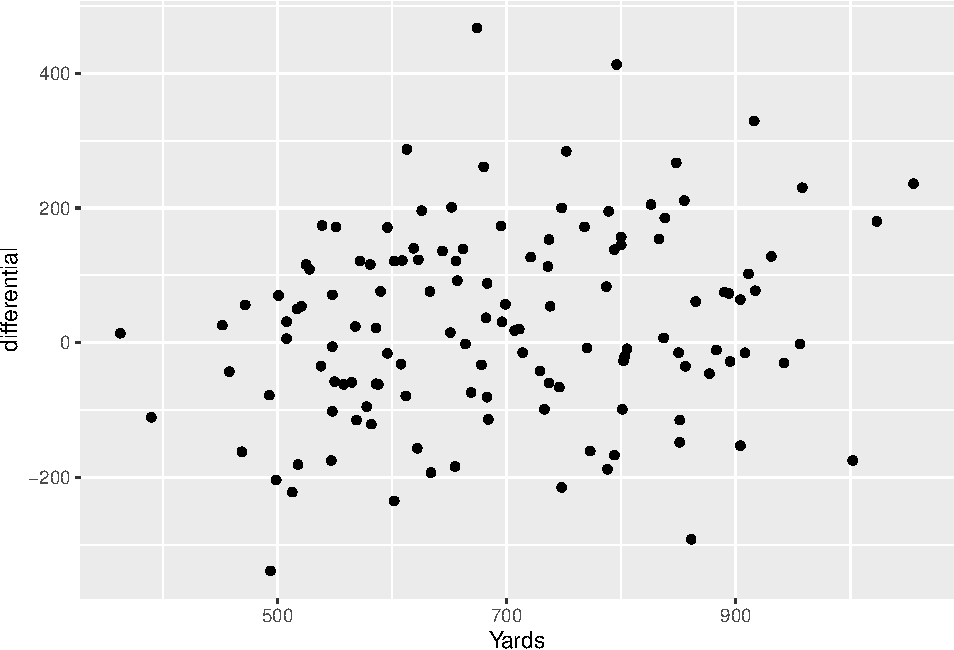
\includegraphics{SportsData_files/figure-latex/unnamed-chunk-61-1.pdf}

\begin{quote}
\textbf{Your turn}: Try it with the other penalty measures. Total penalties and penalty yards per game. Does anything change? Do either of these meet the .05 threshold for randomness? Are either of these any more predictive?
\end{quote}

\hypertarget{a-more-predictive-example}{%
\section{A more predictive example}\label{a-more-predictive-example}}

So we've firmly established that penalties aren't predictive. But what is? One measure I've found to be highly predictive of a team's success is how well do they do on third down. It's simple really: Succeed on third down, you get to stay on offense. Fail on third down, you are punting (most likely) or settling for a field goal. Either way, you're scoring less than you would by scoring touchdowns. How related are points per game and third down conversion percentage?

\begin{Shaded}
\begin{Highlighting}[]
\NormalTok{newcorrelations }\OperatorTok\StringTok{ }
\StringTok{  }\KeywordTok{summarise}\NormalTok{(}\DataTypeTok{correlation =} \KeywordTok{cor}\NormalTok{(OffPointsG, OffConversionPct, }\DataTypeTok{method=}\StringTok{"pearson"}\NormalTok{))}
\end{Highlighting}
\end{Shaded}

\begin{verbatim}
## # A tibble: 1 x 1
##   correlation
##         <dbl>
## 1       0.666
\end{verbatim}

Answer: 67 percent. More than three times more related than penalty yards. But how meaningful is that relationship and how predictive is it?

\begin{Shaded}
\begin{Highlighting}[]
\NormalTok{third <-}\StringTok{ }\KeywordTok{lm}\NormalTok{(OffPointsG }\OperatorTok{~}\StringTok{ }\NormalTok{OffConversionPct, }\DataTypeTok{data =}\NormalTok{ newcorrelations)}
\KeywordTok{summary}\NormalTok{(third)}
\end{Highlighting}
\end{Shaded}

\begin{verbatim}
## 
## Call:
## lm(formula = OffPointsG ~ OffConversionPct, data = newcorrelations)
## 
## Residuals:
##      Min       1Q   Median       3Q      Max 
## -11.3861  -3.5411  -0.5885   2.9011  13.5188 
## 
## Coefficients:
##                  Estimate Std. Error t value Pr(>|t|)    
## (Intercept)      -4.74024    3.41041   -1.39    0.167    
## OffConversionPct  0.85625    0.08479   10.10   <2e-16 ***
## ---
## Signif. codes:  0 '***' 0.001 '**' 0.01 '*' 0.05 '.' 0.1 ' ' 1
## 
## Residual standard error: 5.111 on 128 degrees of freedom
## Multiple R-squared:  0.4434, Adjusted R-squared:  0.4391 
## F-statistic:   102 on 1 and 128 DF,  p-value: < 2.2e-16
\end{verbatim}

First we check p-value. See that e-16? That means scientific notation. That means our number is 2.2 times 10 to the -16 power. So -.000000000000000022. That's sixteen zeros between the decimal and 22. Is that less than .05? Uh, yeah. So this is really, really, really not random. But anyone who has watched a game of football knows this is true. It makes intuitive sense.

Second, Adjusted R-squared: .4391. So we can predict 44 percent of the difference in the total offensive points per game a team scores by simply looking at their third down conversion percentage.

Third, the coefficients: In this case, our \texttt{y=mx+b} formula looks like \texttt{y\ =\ .85625x-4.74024}. So if we were applying this, let's look at Nebraska's 31-28 loss to Iowa on Black Friday in 2018. Nebraska was 6-15 on third down in that game, or 40 percent (Iowa was 7 of 13 or 54 percent). Given those numbers, our formula predicts Nebraska should have scored how many points?

\begin{Shaded}
\begin{Highlighting}[]
\NormalTok{(}\FloatTok{0.85625} \OperatorTok{*}\StringTok{ }\DecValTok{40}\NormalTok{) }\OperatorTok{-}\StringTok{ }\FloatTok{4.74024} 
\end{Highlighting}
\end{Shaded}

\begin{verbatim}
## [1] 29.50976
\end{verbatim}

That's really close to the 28 they did score. And Iowa?

\begin{Shaded}
\begin{Highlighting}[]
\NormalTok{(}\FloatTok{0.85625} \OperatorTok{*}\StringTok{ }\DecValTok{54}\NormalTok{) }\OperatorTok{-}\StringTok{ }\FloatTok{4.74024} 
\end{Highlighting}
\end{Shaded}

\begin{verbatim}
## [1] 41.49726
\end{verbatim}

By our model, Iowa should have scored 10 more points than they did. But they didn't. Why, besides Iowa is terrible and deserves punishment from the football gods for being Iowa? Remember our model can only explain 44 percent of the points. There's more to football than one metric.

\hypertarget{multiple-regression}{%
\chapter{Multiple regression}\label{multiple-regression}}

Last chapter, we looked at correlations and linear regression to predict how one element of a game would predict the score. But we know that a single variable, in all but the rarest instances, are not going to be that predictive. We need more than one. Enter multiple regression. Multiple regression lets us add -- wait for it -- multiple predictors to our equation to help us get a better

That presents it's own problems. So let's get our libraries and our data, this time of \href{https://unl.box.com/s/u9407jj007fxtnu1vbkybdawaqg6j3fw}{every college basketball game since the 2014-15 season} loaded up.

\begin{Shaded}
\begin{Highlighting}[]
\KeywordTok{library}\NormalTok{(tidyverse)}
\end{Highlighting}
\end{Shaded}

\begin{Shaded}
\begin{Highlighting}[]
\NormalTok{logs <-}\StringTok{ }\KeywordTok{read_csv}\NormalTok{(}\StringTok{"data/logs1519.csv"}\NormalTok{)}
\end{Highlighting}
\end{Shaded}

\begin{verbatim}
## Warning: Missing column names filled in: 'X1' [1]
\end{verbatim}

\begin{verbatim}
## Parsed with column specification:
## cols(
##   .default = col_double(),
##   Date = col_date(format = ""),
##   HomeAway = col_character(),
##   Opponent = col_character(),
##   W_L = col_character(),
##   Blank = col_logical(),
##   Team = col_character(),
##   Conference = col_character(),
##   season = col_character()
## )
\end{verbatim}

\begin{verbatim}
## See spec(...) for full column specifications.
\end{verbatim}

So one way to show how successful a basketball team was for a game is to show the differential between the team's score and the opponent's score. Score a lot more than the opponent = good, score a lot less than the opponent = bad. And, relatively speaking, the more the better. So let's create that differential.

\begin{Shaded}
\begin{Highlighting}[]
\NormalTok{logs <-}\StringTok{ }\NormalTok{logs }\OperatorTok\StringTok{ }\KeywordTok{mutate}\NormalTok{(}\DataTypeTok{Differential =}\NormalTok{ TeamScore }\OperatorTok{-}\StringTok{ }\NormalTok{OpponentScore)}
\end{Highlighting}
\end{Shaded}

The linear model code we used before is pretty straight forward. Its \texttt{field} is predicted by \texttt{field}. Here's a simple linear model that looks at predicting a team's point differential by looking at their offensive shooting percentage.

\begin{Shaded}
\begin{Highlighting}[]
\NormalTok{shooting <-}\StringTok{ }\KeywordTok{lm}\NormalTok{(TeamFGPCT }\OperatorTok{~}\StringTok{ }\NormalTok{Differential, }\DataTypeTok{data=}\NormalTok{logs)}
\KeywordTok{summary}\NormalTok{(shooting)}
\end{Highlighting}
\end{Shaded}

\begin{verbatim}
## 
## Call:
## lm(formula = TeamFGPCT ~ Differential, data = logs)
## 
## Residuals:
##       Min        1Q    Median        3Q       Max 
## -0.260485 -0.040230 -0.001096  0.039038  0.267457 
## 
## Coefficients:
##               Estimate Std. Error t value Pr(>|t|)    
## (Intercept)  4.399e-01  2.487e-04  1768.4   <2e-16 ***
## Differential 2.776e-03  1.519e-05   182.8   <2e-16 ***
## ---
## Signif. codes:  0 '***' 0.001 '**' 0.01 '*' 0.05 '.' 0.1 ' ' 1
## 
## Residual standard error: 0.05949 on 57514 degrees of freedom
##   (4 observations deleted due to missingness)
## Multiple R-squared:  0.3675, Adjusted R-squared:  0.3674 
## F-statistic: 3.341e+04 on 1 and 57514 DF,  p-value: < 2.2e-16
\end{verbatim}

Remember: There's a lot here, but only some of it we care about. What is the Adjusted R-squared value? What's the p-value and is it less than .05? In this case, we can predict 37 percent of the difference in differential with how well a team shoots the ball.

To add more predictors to this mix, we merely add them. But it's not that simple, as you'll see in a moment. So first, let's look at adding how well the other team shot to our prediction model:

\begin{Shaded}
\begin{Highlighting}[]
\NormalTok{model1 <-}\StringTok{ }\KeywordTok{lm}\NormalTok{(Differential }\OperatorTok{~}\StringTok{ }\NormalTok{TeamFGPCT }\OperatorTok{+}\StringTok{ }\NormalTok{OpponentFGPCT, }\DataTypeTok{data=}\NormalTok{logs)}
\KeywordTok{summary}\NormalTok{(model1)}
\end{Highlighting}
\end{Shaded}

\begin{verbatim}
## 
## Call:
## lm(formula = Differential ~ TeamFGPCT + OpponentFGPCT, data = logs)
## 
## Residuals:
##     Min      1Q  Median      3Q     Max 
## -49.591  -6.185  -0.198   5.938  68.344 
## 
## Coefficients:
##                Estimate Std. Error  t value Pr(>|t|)    
## (Intercept)      1.1195     0.3483    3.214  0.00131 ** 
## TeamFGPCT      118.5211     0.5279  224.518  < 2e-16 ***
## OpponentFGPCT -119.9369     0.5252 -228.372  < 2e-16 ***
## ---
## Signif. codes:  0 '***' 0.001 '**' 0.01 '*' 0.05 '.' 0.1 ' ' 1
## 
## Residual standard error: 9.407 on 57513 degrees of freedom
##   (4 observations deleted due to missingness)
## Multiple R-squared:  0.6683, Adjusted R-squared:  0.6683 
## F-statistic: 5.793e+04 on 2 and 57513 DF,  p-value: < 2.2e-16
\end{verbatim}

First things first: What is the adjusted R-squared?

Second: what is the p-value and is it less than .05?

Third: Compare the residual standard error. We went from .05949 to 9.4. The meaning of this is both really opaque and also simple -- we added a lot of error to our model by adding more measures -- 158 times more. Residual standard error is the total distance between what our model would predict and what we actually have in the data. So lots of residual error means the distance between reality and our model is wider. So the width of our predictive range in this example grew pretty dramatically, but so did the amount of the difference we could predict. It's a trade off.

One of the more difficult things to understand about multiple regression is the issue of multicollinearity. What that means is that there is significant correlation overlap between two variables -- the two are related to each other as well as to the target output -- and all you are doing by adding both of them is adding error with no real value to the R-squared. In pure statistics, we don't want any multicollinearity at all. Violating that assumption limits the applicability of what you are doing. So if we have some multicollinearity, it limits our scope of application to college basketball. We can't say this will work for every basketball league and level everywhere. What we need to do is see how correlated each value is to each other and throw out ones that are highly co-correlated.

So to find those, we have to create a correlation matrix that shows us how each value is correlated to our outcome variable, but also with each other. We can do that in the \texttt{Hmisc} library. We install that in the console with \texttt{install.packages("Hmisc")}

\begin{Shaded}
\begin{Highlighting}[]
\KeywordTok{library}\NormalTok{(Hmisc)}
\end{Highlighting}
\end{Shaded}

We can pass in every numeric value to the Hmisc library and get a correlation matrix out of it, but since we have a large number of values -- and many of them character values -- we should strip that down and reorder them. So that's what I'm doing here. I'm saying give me differential first, and then columns 9-24, and then 26-41. Why the skip? There's a blank column in the middle of the data -- a remnant of the scraper I used.

\begin{Shaded}
\begin{Highlighting}[]
\NormalTok{simplelogs <-}\StringTok{ }\NormalTok{logs }\OperatorTok\StringTok{ }\KeywordTok{select}\NormalTok{(Differential, }\DecValTok{9}\OperatorTok{:}\DecValTok{24}\NormalTok{, }\DecValTok{26}\OperatorTok{:}\DecValTok{41}\NormalTok{)}
\end{Highlighting}
\end{Shaded}

Before we proceed, what we're looking to do is follow the Differential column down, looking for correlation values near 1 or -1. Correlations go from -1, meaning perfect negative correlation, to 0, meaning no correlation, to 1, meaning perfect positive correlation. So we're looking for numbers near 1 or -1 for their predictive value. BUT: We then need to see if that value is also highly correlated with something else. If it is, we have a decision to make.

We get our correlation matrix like this:

\begin{Shaded}
\begin{Highlighting}[]
\NormalTok{cormatrix <-}\StringTok{ }\KeywordTok{rcorr}\NormalTok{(}\KeywordTok{as.matrix}\NormalTok{(simplelogs))}

\NormalTok{cormatrix}\OperatorTok{$}\NormalTok{r}
\end{Highlighting}
\end{Shaded}

\begin{verbatim}
##                       Differential       TeamFG      TeamFGA    TeamFGPCT
## Differential           1.000000000  0.584766682  0.107389235  0.606178206
## TeamFG                 0.584766682  1.000000000  0.563220974  0.751715176
## TeamFGA                0.107389235  0.563220974  1.000000000 -0.109620267
## TeamFGPCT              0.606178206  0.751715176 -0.109620267  1.000000000
## Team3P                 0.318300418  0.408787900  0.213352219  0.322872202
## Team3PA                0.056680627  0.179527313  0.426011924 -0.119421368
## Team3PPCT              0.367934059  0.380235821 -0.101463821  0.545986963
## TeamFT                 0.238182740 -0.022308582 -0.137853824  0.084649669
## TeamFTA                0.206075949 -0.027927391 -0.129851346  0.070632302
## TeamFTPCT              0.138833800  0.016247282 -0.044394472  0.056887587
## TeamOffRebounds        0.136095147  0.161626257  0.545231683 -0.234244567
## TeamTotalRebounds      0.470722398  0.328460524  0.470719037  0.018581908
## TeamAssists            0.540398009  0.664057724  0.284659104  0.566152928
## TeamSteals             0.277670288  0.210221346  0.208743124  0.080191710
## TeamBlocks             0.257608076  0.140856644  0.074555286  0.107327505
## TeamTurnovers         -0.180578328 -0.143210529 -0.223971265  0.001901048
## TeamPersonalFouls     -0.194427271 -0.014722266  0.107325560 -0.094653222
## OpponentFG            -0.538515115  0.144061400  0.256737262 -0.020183466
## OpponentFGA            0.001768386  0.302143806  0.301593528  0.126415534
## OpponentFGPCT         -0.614427717 -0.058571888  0.068034775 -0.114791403
## Opponent3P            -0.283754971  0.131517138  0.135290090  0.053105214
## Opponent3PA            0.013910296  0.191131927  0.138445785  0.118723805
## Opponent3PPCT         -0.382427841  0.008026622  0.057261756 -0.031370545
## OpponentFT            -0.269300868  0.019511923  0.157025930 -0.091558712
## OpponentFTA           -0.226064714  0.012937366  0.159529646 -0.101685664
## OpponentFTPCT         -0.175223632  0.007923359  0.023732217 -0.006190565
## OpponentOffRebounds   -0.089347536 -0.036316958  0.002848058 -0.042399744
## OpponentTotalRebounds -0.420010794 -0.225202127  0.316139528 -0.512983306
## OpponentAssists       -0.491676030  0.004558539  0.149320067 -0.106252682
## OpponentSteals        -0.187754380 -0.102436608 -0.131734964 -0.021724636
## OpponentBlocks        -0.262252627 -0.160469663  0.218483865 -0.356255034
## OpponentTurnovers      0.274326954  0.155293275  0.198127970  0.024254833
## OpponentPersonalFouls  0.169025733 -0.023116620 -0.107189301  0.060150658
##                             Team3P     Team3PA     Team3PPCT       TeamFT
## Differential           0.318300418  0.05668063  0.3679340589  0.238182740
## TeamFG                 0.408787900  0.17952731  0.3802358207 -0.022308582
## TeamFGA                0.213352219  0.42601192 -0.1014638212 -0.137853824
## TeamFGPCT              0.322872202 -0.11942137  0.5459869634  0.084649669
## Team3P                 1.000000000  0.70114773  0.7073663404 -0.106344056
## Team3PA                0.701147726  1.00000000  0.0407645751 -0.160515313
## Team3PPCT              0.707366340  0.04076458  1.0000000000  0.005129556
## TeamFT                -0.106344056 -0.16051531  0.0051295561  1.000000000
## TeamFTA               -0.137499074 -0.18150913 -0.0180696209  0.927525817
## TeamFTPCT              0.048777304  0.01119250  0.0553684315  0.387017653
## TeamOffRebounds       -0.062026229  0.12484929 -0.1968568361  0.087168289
## TeamTotalRebounds      0.038344971  0.12095682 -0.0628970009  0.190691619
## TeamAssists            0.519530086  0.28786139  0.4326950943 -0.016343370
## TeamSteals             0.016545254  0.04598400 -0.0246657289  0.088535320
## TeamBlocks             0.004747719 -0.02895321  0.0294277389  0.092392379
## TeamTurnovers         -0.088374940 -0.10883919 -0.0209433827  0.051609207
## TeamPersonalFouls     -0.024028303  0.02499520 -0.0498165852  0.217846416
## OpponentFG             0.123800594  0.15638030  0.0296913406  0.057853338
## OpponentFGA            0.148931744  0.13062824  0.0812237901  0.193116094
## OpponentFGPCT          0.029908235  0.08057726 -0.0264843759 -0.075399282
## Opponent3P             0.079455775  0.07482590  0.0402012413  0.024228311
## Opponent3PA            0.085704376  0.05927299  0.0601150176  0.079894905
## Opponent3PPCT          0.029666235  0.04634676  0.0005076038 -0.035478488
## OpponentFT             0.009796521  0.06316300 -0.0390873639  0.161311559
## OpponentFTA           -0.002503282  0.05474884 -0.0480732723  0.183801456
## OpponentFTPCT          0.022780414  0.02587876  0.0086512859 -0.015688533
## OpponentOffRebounds   -0.007870292 -0.01895081  0.0086776821  0.064938518
## OpponentTotalRebounds -0.062384273  0.20289676 -0.2638845414 -0.064969878
## OpponentAssists        0.029413582  0.08254506 -0.0320289494 -0.057730062
## OpponentSteals        -0.053878305 -0.05298037 -0.0251316716 -0.001883349
## OpponentBlocks        -0.111782062 -0.05804217 -0.0965607977 -0.065055523
## OpponentTurnovers      0.009284106  0.06383515 -0.0488449748  0.136922084
## OpponentPersonalFouls -0.127197007 -0.15536393 -0.0268876881  0.793539202
##                            TeamFTA    TeamFTPCT TeamOffRebounds
## Differential           0.206075949  0.138833800    0.1360951470
## TeamFG                -0.027927391  0.016247282    0.1616262575
## TeamFGA               -0.129851346 -0.044394472    0.5452316831
## TeamFGPCT              0.070632302  0.056887587   -0.2342445674
## Team3P                -0.137499074  0.048777304   -0.0620262290
## Team3PA               -0.181509133  0.011192503    0.1248492948
## Team3PPCT             -0.018069621  0.055368431   -0.1968568361
## TeamFT                 0.927525817  0.387017653    0.0871682888
## TeamFTA                1.000000000  0.053233778    0.1415933172
## TeamFTPCT              0.053233778  1.000000000   -0.0948040467
## TeamOffRebounds        0.141593317 -0.094804047    1.0000000000
## TeamTotalRebounds      0.231278690 -0.037356471    0.6373027887
## TeamAssists           -0.028289202  0.025948025    0.0509277222
## TeamSteals             0.111199125 -0.025969502    0.1195581042
## TeamBlocks             0.104112579 -0.001425412    0.1060163877
## TeamTurnovers          0.072070652 -0.034614485    0.0371728710
## TeamPersonalFouls      0.250787085 -0.025827923    0.0542337992
## OpponentFG             0.043602296  0.036986356   -0.0464694335
## OpponentFGA            0.193466766  0.040334507    0.0242353640
## OpponentFGPCT         -0.091897172  0.012864509   -0.0688833747
## Opponent3P             0.009600704  0.031763685   -0.0063710321
## Opponent3PA            0.071193179  0.032554796    0.0003753868
## Opponent3PPCT         -0.047136861  0.013996880   -0.0056578317
## OpponentFT             0.180010001 -0.009352580    0.0434399899
## OpponentFTA            0.213209437 -0.025707797    0.0584669041
## OpponentFTPCT         -0.032862991  0.028078614   -0.0319032781
## OpponentOffRebounds    0.077003661 -0.016936223   -0.0143325753
## OpponentTotalRebounds  0.004736343 -0.177541483   -0.0603891339
## OpponentAssists       -0.063875391 -0.007401206   -0.0386521955
## OpponentSteals         0.006758108 -0.022033431    0.0326977763
## OpponentBlocks        -0.053973588 -0.041175463    0.1571812909
## OpponentTurnovers      0.169704736 -0.035463921    0.1154717115
## OpponentPersonalFouls  0.866395092  0.018757079    0.1240631120
##                       TeamTotalRebounds   TeamAssists   TeamSteals   TeamBlocks
## Differential                0.470722398  0.5403980088  0.277670288  0.257608076
## TeamFG                      0.328460524  0.6640577242  0.210221346  0.140856644
## TeamFGA                     0.470719037  0.2846591045  0.208743124  0.074555286
## TeamFGPCT                   0.018581908  0.5661529279  0.080191710  0.107327505
## Team3P                      0.038344971  0.5195300862  0.016545254  0.004747719
## Team3PA                     0.120956819  0.2878613903  0.045984003 -0.028953212
## Team3PPCT                  -0.062897001  0.4326950943 -0.024665729  0.029427739
## TeamFT                      0.190691619 -0.0163433697  0.088535320  0.092392379
## TeamFTA                     0.231278690 -0.0282892019  0.111199125  0.104112579
## TeamFTPCT                  -0.037356471  0.0259480253 -0.025969502 -0.001425412
## TeamOffRebounds             0.637302789  0.0509277222  0.119558104  0.106016388
## TeamTotalRebounds           1.000000000  0.2321524530  0.027446991  0.265518873
## TeamAssists                 0.232152453  1.0000000000  0.164837110  0.144764562
## TeamSteals                  0.027446991  0.1648371104  1.000000000  0.065539758
## TeamBlocks                  0.265518873  0.1447645615  0.065539758  1.000000000
## TeamTurnovers               0.109155292 -0.0789200586  0.078278779  0.032775757
## TeamPersonalFouls          -0.007423332 -0.1050900267  0.005151965 -0.054105029
## OpponentFG                 -0.229331788 -0.0022308763 -0.138728115 -0.143969401
## OpponentFGA                 0.360268614  0.1863368268 -0.120696505  0.257245080
## OpponentFGPCT              -0.530432484 -0.1397140493 -0.068951590 -0.353110391
## Opponent3P                 -0.053371243  0.0354785684 -0.062074442 -0.103465578
## Opponent3PA                 0.232049186  0.1116023406 -0.039184667 -0.042234814
## Opponent3PPCT              -0.273572339 -0.0502063543 -0.047114732 -0.099440199
## OpponentFT                 -0.095266106 -0.0835716395 -0.034152581 -0.070920662
## OpponentFTA                -0.022971823 -0.0841605708 -0.022178476 -0.056095076
## OpponentFTPCT              -0.194279344 -0.0278263543 -0.041125993 -0.052504157
## OpponentOffRebounds        -0.052416263 -0.0333847454  0.016707012  0.178200671
## OpponentTotalRebounds      -0.059965631 -0.2225952122  0.035155522  0.037788375
## OpponentAssists            -0.218597433  0.0006884142 -0.053327136 -0.151146052
## OpponentSteals              0.066119486 -0.0288668673  0.055697260  0.028453380
## OpponentBlocks              0.013924890 -0.1657235463 -0.002230784 -0.038978593
## OpponentTurnovers          -0.034355689  0.1314533533  0.730885169  0.031375703
## OpponentPersonalFouls       0.189144014 -0.0267820830  0.071442012  0.080582762
##                       TeamTurnovers TeamPersonalFouls   OpponentFG  OpponentFGA
## Differential           -0.180578328      -0.194427271 -0.538515115  0.001768386
## TeamFG                 -0.143210529      -0.014722266  0.144061400  0.302143806
## TeamFGA                -0.223971265       0.107325560  0.256737262  0.301593528
## TeamFGPCT               0.001901048      -0.094653222 -0.020183466  0.126415534
## Team3P                 -0.088374940      -0.024028303  0.123800594  0.148931744
## Team3PA                -0.108839191       0.024995197  0.156380301  0.130628244
## Team3PPCT              -0.020943383      -0.049816585  0.029691341  0.081223790
## TeamFT                  0.051609207       0.217846416  0.057853338  0.193116094
## TeamFTA                 0.072070652       0.250787085  0.043602296  0.193466766
## TeamFTPCT              -0.034614485      -0.025827923  0.036986356  0.040334507
## TeamOffRebounds         0.037172871       0.054233799 -0.046469434  0.024235364
## TeamTotalRebounds       0.109155292      -0.007423332 -0.229331788  0.360268614
## TeamAssists            -0.078920059      -0.105090027 -0.002230876  0.186336827
## TeamSteals              0.078278779       0.005151965 -0.138728115 -0.120696505
## TeamBlocks              0.032775757      -0.054105029 -0.143969401  0.257245080
## TeamTurnovers           1.000000000       0.220285924  0.081879049  0.155947902
## TeamPersonalFouls       0.220285924       1.000000000 -0.015422966 -0.122639976
## OpponentFG              0.081879049      -0.015422966  1.000000000  0.515517123
## OpponentFGA             0.155947902      -0.122639976  0.515517123  1.000000000
## OpponentFGPCT          -0.023017156       0.078411084  0.754791141 -0.161220379
## Opponent3P             -0.018088322      -0.126817358  0.399027442  0.193563166
## Opponent3PA             0.041669476      -0.167647391  0.144074778  0.418730422
## Opponent3PPCT          -0.063187150      -0.015909552  0.395540055 -0.118020866
## OpponentFT              0.123594852       0.793147614 -0.013421944 -0.156152803
## OpponentFTA             0.154110278       0.865844664 -0.027151720 -0.151706668
## OpponentFTPCT          -0.034267574       0.026877590  0.037049836 -0.043324702
## OpponentOffRebounds     0.074131214       0.122282037  0.120715447  0.519792207
## OpponentTotalRebounds  -0.106168146       0.195017438  0.275438081  0.424276325
## OpponentAssists         0.072644677      -0.022619097  0.638304131  0.231851475
## OpponentSteals          0.709987911       0.064446997  0.140823916  0.165329579
## OpponentBlocks          0.006463872       0.087211248  0.129076992  0.045565883
## OpponentTurnovers       0.188537020       0.101693555 -0.183558009 -0.215633733
## OpponentPersonalFouls   0.131539040       0.322258517  0.015334210  0.136789046
##                       OpponentFGPCT   Opponent3P   Opponent3PA Opponent3PPCT
## Differential           -0.614427717 -0.283754971  0.0139102958 -0.3824278411
## TeamFG                 -0.058571888  0.131517138  0.1911319274  0.0080266219
## TeamFGA                 0.068034775  0.135290090  0.1384457845  0.0572617563
## TeamFGPCT              -0.114791403  0.053105214  0.1187238045 -0.0313705446
## Team3P                  0.029908235  0.079455775  0.0857043764  0.0296662353
## Team3PA                 0.080577258  0.074825900  0.0592729911  0.0463467602
## Team3PPCT              -0.026484376  0.040201241  0.0601150176  0.0005076038
## TeamFT                 -0.075399282  0.024228311  0.0798949051 -0.0354784876
## TeamFTA                -0.091897172  0.009600704  0.0711931792 -0.0471368607
## TeamFTPCT               0.012864509  0.031763685  0.0325547961  0.0139968801
## TeamOffRebounds        -0.068883375 -0.006371032  0.0003753868 -0.0056578317
## TeamTotalRebounds      -0.530432484 -0.053371243  0.2320491861 -0.2735723395
## TeamAssists            -0.139714049  0.035478568  0.1116023406 -0.0502063543
## TeamSteals             -0.068951590 -0.062074442 -0.0391846669 -0.0471147320
## TeamBlocks             -0.353110391 -0.103465578 -0.0422348142 -0.0994401990
## TeamTurnovers          -0.023017156 -0.018088322  0.0416694763 -0.0631871498
## TeamPersonalFouls       0.078411084 -0.126817358 -0.1676473908 -0.0159095518
## OpponentFG              0.754791141  0.399027442  0.1440747785  0.3955400546
## OpponentFGA            -0.161220379  0.193563166  0.4187304220 -0.1180208656
## OpponentFGPCT           1.000000000  0.312295571 -0.1493674362  0.5522792378
## Opponent3P              0.312295571  1.000000000  0.6914518201  0.7094041257
## Opponent3PA            -0.149367436  0.691451820  1.0000000000  0.0303822862
## Opponent3PPCT           0.552279238  0.709404126  0.0303822862  1.0000000000
## OpponentFT              0.106226566 -0.106344743 -0.1743400433  0.0169282910
## OpponentFTA             0.086625216 -0.140194309 -0.1972872368 -0.0080249496
## OpponentFTPCT           0.076650746  0.053774302  0.0101886734  0.0623587723
## OpponentOffRebounds    -0.251623986 -0.085432899  0.0978389488 -0.2013096986
## OpponentTotalRebounds  -0.005789348  0.005903551  0.0810576009 -0.0680836101
## OpponentAssists         0.553535793  0.513869716  0.2641728450  0.4428640799
## OpponentSteals          0.036468797 -0.011661373  0.0214481397 -0.0383569868
## OpponentBlocks          0.111935521 -0.004746412 -0.0495426307  0.0354134646
## OpponentTurnovers      -0.048082678 -0.095218199 -0.0944428800 -0.0421344973
## OpponentPersonalFouls  -0.081776664 -0.011247805  0.0396475169 -0.0466461289
##                         OpponentFT  OpponentFTA OpponentFTPCT
## Differential          -0.269300868 -0.226064714  -0.175223632
## TeamFG                 0.019511923  0.012937366   0.007923359
## TeamFGA                0.157025930  0.159529646   0.023732217
## TeamFGPCT             -0.091558712 -0.101685664  -0.006190565
## Team3P                 0.009796521 -0.002503282   0.022780414
## Team3PA                0.063163000  0.054748838   0.025878762
## Team3PPCT             -0.039087364 -0.048073272   0.008651286
## TeamFT                 0.161311559  0.183801456  -0.015688533
## TeamFTA                0.180010001  0.213209437  -0.032862991
## TeamFTPCT             -0.009352580 -0.025707797   0.028078614
## TeamOffRebounds        0.043439990  0.058466904  -0.031903278
## TeamTotalRebounds     -0.095266106 -0.022971823  -0.194279344
## TeamAssists           -0.083571639 -0.084160571  -0.027826354
## TeamSteals            -0.034152581 -0.022178476  -0.041125993
## TeamBlocks            -0.070920662 -0.056095076  -0.052504157
## TeamTurnovers          0.123594852  0.154110278  -0.034267574
## TeamPersonalFouls      0.793147614  0.865844664   0.026877590
## OpponentFG            -0.013421944 -0.027151720   0.037049836
## OpponentFGA           -0.156152803 -0.151706668  -0.043324702
## OpponentFGPCT          0.106226566  0.086625216   0.076650746
## Opponent3P            -0.106344743 -0.140194309   0.053774302
## Opponent3PA           -0.174340043 -0.197287237   0.010188673
## Opponent3PPCT          0.016928291 -0.008024950   0.062358772
## OpponentFT             1.000000000  0.928286066   0.393203255
## OpponentFTA            0.928286066  1.000000000   0.063446167
## OpponentFTPCT          0.393203255  0.063446167   1.000000000
## OpponentOffRebounds    0.086671729  0.136423744  -0.082982260
## OpponentTotalRebounds  0.197591588  0.232447345  -0.021281750
## OpponentAssists       -0.012378006 -0.031205800   0.041793598
## OpponentSteals         0.077614062  0.097206119  -0.022196700
## OpponentBlocks         0.101422181  0.110063752   0.008946765
## OpponentTurnovers      0.015778567  0.038679394  -0.052040732
## OpponentPersonalFouls  0.215609923  0.251289640  -0.029978048
##                       OpponentOffRebounds OpponentTotalRebounds OpponentAssists
## Differential                 -0.089347536          -0.420010794   -0.4916760300
## TeamFG                       -0.036316958          -0.225202127    0.0045585394
## TeamFGA                       0.002848058           0.316139528    0.1493200670
## TeamFGPCT                    -0.042399744          -0.512983306   -0.1062526818
## Team3P                       -0.007870292          -0.062384273    0.0294135821
## Team3PA                      -0.018950808           0.202896760    0.0825450568
## Team3PPCT                     0.008677682          -0.263884541   -0.0320289494
## TeamFT                        0.064938518          -0.064969878   -0.0577300621
## TeamFTA                       0.077003661           0.004736343   -0.0638753907
## TeamFTPCT                    -0.016936223          -0.177541483   -0.0074012062
## TeamOffRebounds              -0.014332575          -0.060389134   -0.0386521955
## TeamTotalRebounds            -0.052416263          -0.059965631   -0.2185974327
## TeamAssists                  -0.033384745          -0.222595212    0.0006884142
## TeamSteals                    0.016707012           0.035155522   -0.0533271359
## TeamBlocks                    0.178200671           0.037788375   -0.1511460518
## TeamTurnovers                 0.074131214          -0.106168146    0.0726446766
## TeamPersonalFouls             0.122282037           0.195017438   -0.0226190966
## OpponentFG                    0.120715447           0.275438081    0.6383041307
## OpponentFGA                   0.519792207           0.424276325    0.2318514751
## OpponentFGPCT                -0.251623986          -0.005789348    0.5535357935
## Opponent3P                   -0.085432899           0.005903551    0.5138697156
## Opponent3PA                   0.097838949           0.081057601    0.2641728450
## Opponent3PPCT                -0.201309699          -0.068083610    0.4428640799
## OpponentFT                    0.086671729           0.197591588   -0.0123780062
## OpponentFTA                   0.136423744           0.232447345   -0.0312058003
## OpponentFTPCT                -0.082982260          -0.021281750    0.0417935976
## OpponentOffRebounds           1.000000000           0.622115242    0.0095497736
## OpponentTotalRebounds         0.622115242           1.000000000    0.1792668711
## OpponentAssists               0.009549774           0.179266871    1.0000000000
## OpponentSteals                0.081573888          -0.038673692    0.1068223463
## OpponentBlocks                0.096186044           0.258597044    0.1337215898
## OpponentTurnovers             0.017562976           0.073936193   -0.1060361856
## OpponentPersonalFouls         0.071468553           0.020500608   -0.0849725350
##                       OpponentSteals OpponentBlocks OpponentTurnovers
## Differential            -0.187754380  -0.2622526274      0.2743269542
## TeamFG                  -0.102436608  -0.1604696630      0.1552932747
## TeamFGA                 -0.131734964   0.2184838647      0.1981279705
## TeamFGPCT               -0.021724636  -0.3562550337      0.0242548332
## Team3P                  -0.053878305  -0.1117820624      0.0092841059
## Team3PA                 -0.052980367  -0.0580421730      0.0638351465
## Team3PPCT               -0.025131672  -0.0965607977     -0.0488449748
## TeamFT                  -0.001883349  -0.0650555225      0.1369220844
## TeamFTA                  0.006758108  -0.0539735876      0.1697047361
## TeamFTPCT               -0.022033431  -0.0411754626     -0.0354639208
## TeamOffRebounds          0.032697776   0.1571812909      0.1154717115
## TeamTotalRebounds        0.066119486   0.0139248895     -0.0343556886
## TeamAssists             -0.028866867  -0.1657235463      0.1314533533
## TeamSteals               0.055697260  -0.0022307839      0.7308851693
## TeamBlocks               0.028453380  -0.0389785933      0.0313757033
## TeamTurnovers            0.709987911   0.0064638717      0.1885370196
## TeamPersonalFouls        0.064446997   0.0872112484      0.1016935547
## OpponentFG               0.140823916   0.1290769921     -0.1835580089
## OpponentFGA              0.165329579   0.0455658832     -0.2156337333
## OpponentFGPCT            0.036468797   0.1119355214     -0.0480826780
## Opponent3P              -0.011661373  -0.0047464115     -0.0952181989
## Opponent3PA              0.021448140  -0.0495426307     -0.0944428800
## Opponent3PPCT           -0.038356987   0.0354134646     -0.0421344973
## OpponentFT               0.077614062   0.1014221807      0.0157785673
## OpponentFTA              0.097206119   0.1100637520      0.0386793945
## OpponentFTPCT           -0.022196700   0.0089467648     -0.0520407316
## OpponentOffRebounds      0.081573888   0.0961860439      0.0175629757
## OpponentTotalRebounds   -0.038673692   0.2585970440      0.0739361927
## OpponentAssists          0.106822346   0.1337215898     -0.1060361856
## OpponentSteals           1.000000000   0.0443672204      0.0740678539
## OpponentBlocks           0.044367220   1.0000000000      0.0001223389
## OpponentTurnovers        0.074067854   0.0001223389      1.0000000000
## OpponentPersonalFouls    0.030766974  -0.0514541037      0.2252310703
##                       OpponentPersonalFouls
## Differential                     0.16902573
## TeamFG                          -0.02311662
## TeamFGA                         -0.10718930
## TeamFGPCT                        0.06015066
## Team3P                          -0.12719701
## Team3PA                         -0.15536393
## Team3PPCT                       -0.02688769
## TeamFT                           0.79353920
## TeamFTA                          0.86639509
## TeamFTPCT                        0.01875708
## TeamOffRebounds                  0.12406311
## TeamTotalRebounds                0.18914401
## TeamAssists                     -0.02678208
## TeamSteals                       0.07144201
## TeamBlocks                       0.08058276
## TeamTurnovers                    0.13153904
## TeamPersonalFouls                0.32225852
## OpponentFG                       0.01533421
## OpponentFGA                      0.13678905
## OpponentFGPCT                   -0.08177666
## Opponent3P                      -0.01124781
## Opponent3PA                      0.03964752
## Opponent3PPCT                   -0.04664613
## OpponentFT                       0.21560992
## OpponentFTA                      0.25128964
## OpponentFTPCT                   -0.02997805
## OpponentOffRebounds              0.07146855
## OpponentTotalRebounds            0.02050061
## OpponentAssists                 -0.08497254
## OpponentSteals                   0.03076697
## OpponentBlocks                  -0.05145410
## OpponentTurnovers                0.22523107
## OpponentPersonalFouls            1.00000000
\end{verbatim}

Notice right away -- TeamFG is highly correlated. But it's also highly correlated with TeamFGPCT. And that makes sense. A team that doesn't shoot many shots is not going to have a high score differential. But the number of shots taken and the field goal percentage are also highly related. So including both of these measures would be pointless -- they would add error without adding much in the way of predictive power.

\begin{quote}
\textbf{Your turn}: What else do you see? What other values have predictive power and aren't co-correlated?
\end{quote}

We can add more just by simply adding them.

\begin{Shaded}
\begin{Highlighting}[]
\NormalTok{model2 <-}\StringTok{ }\KeywordTok{lm}\NormalTok{(Differential }\OperatorTok{~}\StringTok{ }\NormalTok{TeamFGPCT }\OperatorTok{+}\StringTok{ }\NormalTok{OpponentFGPCT }\OperatorTok{+}\StringTok{ }\NormalTok{TeamTotalRebounds }\OperatorTok{+}\StringTok{ }\NormalTok{OpponentTotalRebounds, }\DataTypeTok{data=}\NormalTok{logs)}
\KeywordTok{summary}\NormalTok{(model2)}
\end{Highlighting}
\end{Shaded}

\begin{verbatim}
## 
## Call:
## lm(formula = Differential ~ TeamFGPCT + OpponentFGPCT + TeamTotalRebounds + 
##     OpponentTotalRebounds, data = logs)
## 
## Residuals:
##     Min      1Q  Median      3Q     Max 
## -44.813  -5.586  -0.109   5.453  60.831 
## 
## Coefficients:
##                         Estimate Std. Error  t value Pr(>|t|)    
## (Intercept)            -3.655461   0.606119   -6.031 1.64e-09 ***
## TeamFGPCT             100.880013   0.560363  180.026  < 2e-16 ***
## OpponentFGPCT         -97.563291   0.565004 -172.677  < 2e-16 ***
## TeamTotalRebounds       0.516176   0.006239   82.729  < 2e-16 ***
## OpponentTotalRebounds  -0.436402   0.006448  -67.679  < 2e-16 ***
## ---
## Signif. codes:  0 '***' 0.001 '**' 0.01 '*' 0.05 '.' 0.1 ' ' 1
## 
## Residual standard error: 8.501 on 57511 degrees of freedom
##   (4 observations deleted due to missingness)
## Multiple R-squared:  0.7291, Adjusted R-squared:  0.7291 
## F-statistic: 3.87e+04 on 4 and 57511 DF,  p-value: < 2.2e-16
\end{verbatim}

Go down the list:

What is the Adjusted R-squared now?
What is the p-value and is it less than .05?
What is the Residual standard error?

The final thing we can do with this is predict things. Look at our coefficients table. See the Estimates? We can build a formula from that, same as we did with linear regressions.

\begin{verbatim}
Differential = (TeamFGPCT*100.880013) + (OpponentFGPCT*-97.563291) + (TeamTotalRebounds*0.516176) + (OpponentTotalRebounds*-0.436402) - 3.655461
\end{verbatim}

How does this apply in the real world? Let's pretend for a minute that you are Fred Hoiberg, and you have just been hired as Nebraska's Mens Basketball Coach. Your job is to win conference titles and go deep into the NCAA tournament. To do that, we need to know what attributes of a team should we emphasize. We can do that by looking at what previous Big Ten conference champions looked like.

So if our goal is to predict a conference champion team, we need to know what those teams did. Here's the regular season conference champions in this dataset.

\begin{Shaded}
\begin{Highlighting}[]
\NormalTok{logs }\OperatorTok\StringTok{ }\KeywordTok{filter}\NormalTok{(Team }\OperatorTok{==}\StringTok{ "Michigan State Spartans"} \OperatorTok{&}\StringTok{ }\NormalTok{season }\OperatorTok{==}\StringTok{ "2018-2019"} \OperatorTok{|}\StringTok{ }\NormalTok{Team }\OperatorTok{==}\StringTok{ "Michigan State Spartans"} \OperatorTok{&}\StringTok{ }\NormalTok{season }\OperatorTok{==}\StringTok{ "2017-2018"} \OperatorTok{|}\StringTok{ }\NormalTok{Team }\OperatorTok{==}\StringTok{ "Purdue Boilermakers"} \OperatorTok{&}\StringTok{ }\NormalTok{season }\OperatorTok{==}\StringTok{ "2016-2017"} \OperatorTok{|}\StringTok{ }\NormalTok{Team }\OperatorTok{==}\StringTok{ "Indiana Hoosiers"} \OperatorTok{&}\StringTok{ }\NormalTok{season }\OperatorTok{==}\StringTok{ "2015-2016"} \OperatorTok{|}\StringTok{ }\NormalTok{Team }\OperatorTok{==}\StringTok{ "Wisconsin Badgers"} \OperatorTok{&}\StringTok{ }\NormalTok{season }\OperatorTok{==}\StringTok{ "2014-2015"}\NormalTok{) }\OperatorTok\StringTok{ }\KeywordTok{summarise}\NormalTok{(}\DataTypeTok{avgfgpct =} \KeywordTok{mean}\NormalTok{(TeamFGPCT), }\DataTypeTok{avgoppfgpct=}\KeywordTok{mean}\NormalTok{(OpponentFGPCT), }\DataTypeTok{avgtotrebound =} \KeywordTok{mean}\NormalTok{(TeamTotalRebounds), }\DataTypeTok{avgopptotrebound=}\KeywordTok{mean}\NormalTok{(OpponentTotalRebounds))}
\end{Highlighting}
\end{Shaded}

\begin{verbatim}
## # A tibble: 1 x 4
##   avgfgpct avgoppfgpct avgtotrebound avgopptotrebound
##      <dbl>       <dbl>         <dbl>            <dbl>
## 1    0.489       0.409          35.3             27.2
\end{verbatim}

Now it's just plug and chug.

\begin{Shaded}
\begin{Highlighting}[]
\NormalTok{(}\FloatTok{0.4886133}\OperatorTok{*}\FloatTok{100.880013}\NormalTok{) }\OperatorTok{+}\StringTok{ }\NormalTok{(}\FloatTok{0.4090221}\OperatorTok{*-}\FloatTok{97.563291}\NormalTok{) }\OperatorTok{+}\StringTok{ }\NormalTok{(}\FloatTok{35.29834}\OperatorTok{*}\FloatTok{0.516176}\NormalTok{) }\OperatorTok{+}\StringTok{ }\NormalTok{(}\FloatTok{27.20994}\OperatorTok{*-}\FloatTok{0.436402}\NormalTok{) }\OperatorTok{-}\StringTok{ }\FloatTok{3.655461}
\end{Highlighting}
\end{Shaded}

\begin{verbatim}
## [1] 12.076
\end{verbatim}

So a team with those numbers is going to average scoring 12 more points per game than their opponent.

How does that compare to Nebraska of this past season? The last of the Tim Miles era?

\begin{Shaded}
\begin{Highlighting}[]
\NormalTok{logs }\OperatorTok\StringTok{ }
\StringTok{  }\KeywordTok{filter}\NormalTok{(}
\NormalTok{    Team }\OperatorTok{==}\StringTok{ "Nebraska Cornhuskers"} \OperatorTok{&}\StringTok{ }\NormalTok{season }\OperatorTok{==}\StringTok{ "2018-2019"}
\NormalTok{    ) }\OperatorTok\StringTok{ }
\StringTok{  }\KeywordTok{summarise}\NormalTok{(}
    \DataTypeTok{avgfgpct =} \KeywordTok{mean}\NormalTok{(TeamFGPCT), }
    \DataTypeTok{avgoppfgpct =} \KeywordTok{mean}\NormalTok{(OpponentFGPCT), }
    \DataTypeTok{avgtotrebound =} \KeywordTok{mean}\NormalTok{(TeamTotalRebounds),}
    \DataTypeTok{avgopptotrebound =} \KeywordTok{mean}\NormalTok{(OpponentTotalRebounds)}
\NormalTok{    )}
\end{Highlighting}
\end{Shaded}

\begin{verbatim}
## # A tibble: 1 x 4
##   avgfgpct avgoppfgpct avgtotrebound avgopptotrebound
##      <dbl>       <dbl>         <dbl>            <dbl>
## 1    0.431       0.423          32.5             34.9
\end{verbatim}

\begin{Shaded}
\begin{Highlighting}[]
\NormalTok{(}\FloatTok{0.4305833}\OperatorTok{*}\FloatTok{100.880013}\NormalTok{) }\OperatorTok{+}\StringTok{ }\NormalTok{(}\FloatTok{0.4226667}\OperatorTok{*-}\FloatTok{97.563291}\NormalTok{) }\OperatorTok{+}\StringTok{ }\NormalTok{(}\FloatTok{32.5}\OperatorTok{*}\FloatTok{0.516176}\NormalTok{) }\OperatorTok{+}\StringTok{ }\NormalTok{(}\FloatTok{34.94444}\OperatorTok{*-}\FloatTok{0.436402}\NormalTok{) }\OperatorTok{-}\StringTok{ }\FloatTok{3.655461}
\end{Highlighting}
\end{Shaded}

\begin{verbatim}
## [1] 0.07093015
\end{verbatim}

By this model, it predicted we would outscore our opponent by .07 points over the season. So we'd win slightly more than we'd lose. Nebraska's overall record? 19-17.

\hypertarget{residuals}{%
\chapter{Residuals}\label{residuals}}

When looking at a linear model of your data, there's a measure you need to be aware of called residuals. The residual is the distance between what the model predicted and what the real outcome is. So if your model predicted a team would score 38 points per game given their third down conversion percentage, and they score 45, then your residual is 7. If they had scored 31, then their residual would be -7.

Residuals can tell you severals things, but most importantly is if a linear model the right model for your data. If the residuals appear to be random, then a linear model is appropriate. If they have a pattern, it means something else is going on in your data and a linear model isn't appropriate.

Residuals can also tell you who is underperforming and overperforming the model. Let's take a look at an example we've used regularly this semester -- third down conversion percentage and penalties.

Let's first attach libraries and \href{https://unl.box.com/s/zlxoptqixkt98gubk3i6316qun99l49r}{get some data}. Note: In the rvest steps, I rename the first column because it's blank on the page and then I merge scoring offense to two different tables -- third downs and penalties.

\begin{Shaded}
\begin{Highlighting}[]
\KeywordTok{library}\NormalTok{(tidyverse)}
\end{Highlighting}
\end{Shaded}

\begin{Shaded}
\begin{Highlighting}[]
\NormalTok{offense <-}\StringTok{ }\KeywordTok{read_csv}\NormalTok{(}\StringTok{"data/correlations.csv"}\NormalTok{)}
\end{Highlighting}
\end{Shaded}

\begin{verbatim}
## Parsed with column specification:
## cols(
##   Name = col_character(),
##   OffPoints = col_double(),
##   OffPointsG = col_double(),
##   DefPoints = col_double(),
##   DefPointsG = col_double(),
##   Pen. = col_double(),
##   Yards = col_double(),
##   `Pen./G` = col_double(),
##   OffConversions = col_double(),
##   OffConversionPct = col_double(),
##   DefConversions = col_double(),
##   DefConversionPct = col_double()
## )
\end{verbatim}

First, let's build a linear model and save it as a new dataframe called \texttt{fit}.

\begin{Shaded}
\begin{Highlighting}[]
\NormalTok{fit <-}\StringTok{ }\KeywordTok{lm}\NormalTok{(}\StringTok{`}\DataTypeTok{OffPointsG}\StringTok{`} \OperatorTok{~}\StringTok{ `}\DataTypeTok{OffConversionPct}\StringTok{`}\NormalTok{, }\DataTypeTok{data =}\NormalTok{ offense)}
\KeywordTok{summary}\NormalTok{(fit)}
\end{Highlighting}
\end{Shaded}

\begin{verbatim}
## 
## Call:
## lm(formula = OffPointsG ~ OffConversionPct, data = offense)
## 
## Residuals:
##      Min       1Q   Median       3Q      Max 
## -11.3861  -3.5411  -0.5885   2.9011  13.5188 
## 
## Coefficients:
##                  Estimate Std. Error t value Pr(>|t|)    
## (Intercept)      -4.74024    3.41041   -1.39    0.167    
## OffConversionPct  0.85625    0.08479   10.10   <2e-16 ***
## ---
## Signif. codes:  0 '***' 0.001 '**' 0.01 '*' 0.05 '.' 0.1 ' ' 1
## 
## Residual standard error: 5.111 on 128 degrees of freedom
## Multiple R-squared:  0.4434, Adjusted R-squared:  0.4391 
## F-statistic:   102 on 1 and 128 DF,  p-value: < 2.2e-16
\end{verbatim}

We've seen this output before, but let's review because if you are using scatterplots to make a point, you should do this. First, note the Min and Max residual at the top. A team has underperformed the model by 11.4 points, and a team has overperformed it by 13.5. The median residual, where half are above and half are below, is just slightly under the fit line. Close here is good.

Next: Look at the Adjusted R-squared value. What that says is that 44 percent of a team's scoring output can be predicted by their third down conversion percentage. This is just one year, so that's a little low. If we did this with more years, that would go up.

Last: Look at the p-value. We are looking for a p-value smaller than .05. At .05, we can say that our correlation didn't happen at random. And, in this case, it REALLY didn't happen at random.

What we want to do now is look at those residuals. We can add them to our dataframe like this:

\begin{Shaded}
\begin{Highlighting}[]
\NormalTok{offense}\OperatorTok{$}\NormalTok{predicted <-}\StringTok{ }\KeywordTok{predict}\NormalTok{(fit)}
\NormalTok{offense}\OperatorTok{$}\NormalTok{residuals <-}\StringTok{ }\KeywordTok{residuals}\NormalTok{(fit)}
\end{Highlighting}
\end{Shaded}

Now we can sort our data by those residuals. Sorting in descending order gives us the teams that are overperforming the model.

\begin{Shaded}
\begin{Highlighting}[]
\NormalTok{offense }\OperatorTok\StringTok{ }\KeywordTok{arrange}\NormalTok{(}\KeywordTok{desc}\NormalTok{(residuals))}
\end{Highlighting}
\end{Shaded}

\begin{verbatim}
## # A tibble: 130 x 14
##    Name  OffPoints OffPointsG DefPoints DefPointsG  Pen. Yards `Pen./G`
##    <chr>     <dbl>      <dbl>     <dbl>      <dbl> <dbl> <dbl>    <dbl>
##  1 Tole~       525       40.4       397       30.5    99   931      7.6
##  2 Utah~       618       47.5       289       22.2   101   916      7.8
##  3 Syra~       523       40.2       351       27      94   768      7.2
##  4 Okla~       677       48.4       466       33.3    86   855      6.1
##  5 Clem~       664       44.3       197       13.1    73   674      4.9
##  6 Hous~       571       43.9       483       37.2    87   683      6.7
##  7 Miss~       407       33.9       434       36.2    88   802      7.3
##  8 Neva~       404       31.1       350       26.9    77   738      5.9
##  9 Bost~       384       32         308       25.7    75   590      6.3
## 10 West~       483       40.3       326       27.2    85   800      7.1
## # ... with 120 more rows, and 6 more variables: OffConversions <dbl>,
## #   OffConversionPct <dbl>, DefConversions <dbl>, DefConversionPct <dbl>,
## #   predicted <dbl>, residuals <dbl>
\end{verbatim}

So looking at this table, what you see here are the teams who scored more than their third down conversion percentage would indicate. Some of those teams were just lucky. Some of those teams were really good at long touchdown plays that didn't need a lot of third downs to get down the field. But these are your overperformers.

But, before we can bestow any validity on it, we need to see if this linear model is appropriate. We've done that some looking at our p-values and R-squared values. But one more check is to look at the residuals themselves. We do that by plotting the residuals with the predictor. We'll get into plotting soon, but for now just seeing it is enough.

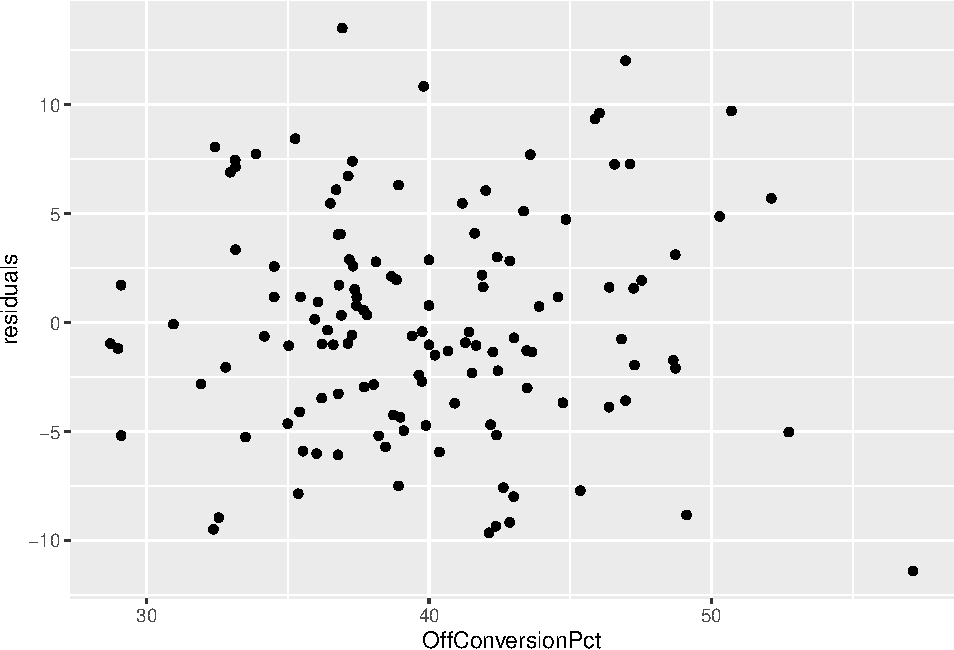
\includegraphics{SportsData_files/figure-latex/unnamed-chunk-84-1.pdf}

The lack of a shape here -- the seemingly random nature -- is a good sign that a linear model works for our data. If there was a pattern, that would indicate something else was going on in our data and we needed a different model.

Another way to view your residuals is by connecting the predicted value with the actual value.

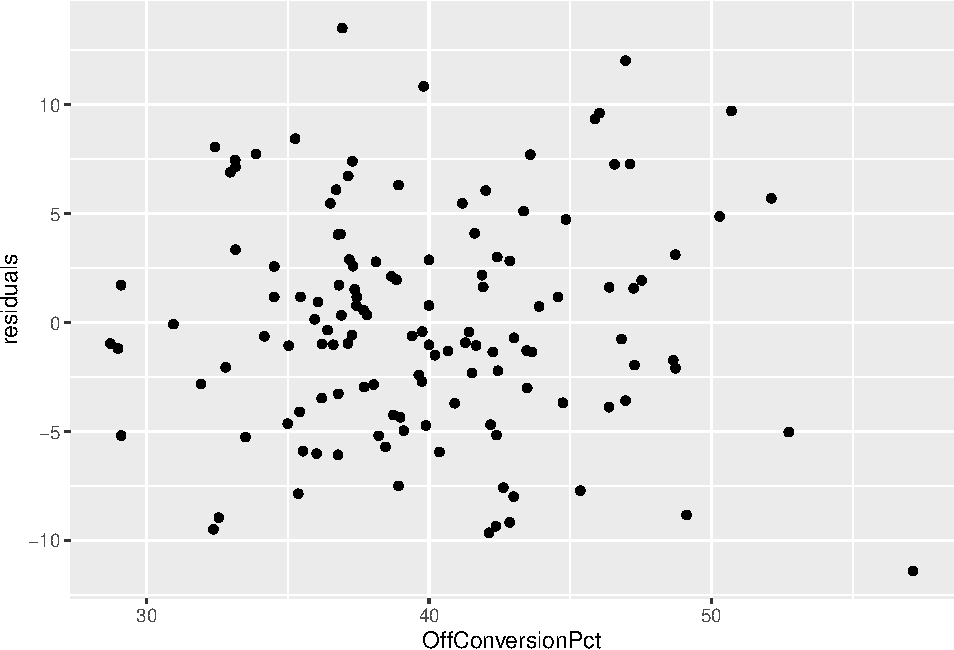
\includegraphics{SportsData_files/figure-latex/unnamed-chunk-85-1.pdf}

The blue line here separates underperformers from overperformers.

\hypertarget{penalties}{%
\section{Penalties}\label{penalties}}

Now let's look at it where it doesn't work: Penalties.

\begin{Shaded}
\begin{Highlighting}[]
\NormalTok{penalties <-}\StringTok{ }\NormalTok{offense}
\end{Highlighting}
\end{Shaded}

\begin{Shaded}
\begin{Highlighting}[]
\NormalTok{pfit <-}\StringTok{ }\KeywordTok{lm}\NormalTok{(OffPointsG }\OperatorTok{~}\StringTok{ }\NormalTok{Yards, }\DataTypeTok{data =}\NormalTok{ penalties)}
\KeywordTok{summary}\NormalTok{(pfit)}
\end{Highlighting}
\end{Shaded}

\begin{verbatim}
## 
## Call:
## lm(formula = OffPointsG ~ Yards, data = penalties)
## 
## Residuals:
##      Min       1Q   Median       3Q      Max 
## -16.5381  -4.5779  -0.5204   4.2418  17.0543 
## 
## Coefficients:
##              Estimate Std. Error t value Pr(>|t|)    
## (Intercept) 20.897213   2.819227   7.412 1.49e-11 ***
## Yards        0.012220   0.003966   3.082  0.00252 ** 
## ---
## Signif. codes:  0 '***' 0.001 '**' 0.01 '*' 0.05 '.' 0.1 ' ' 1
## 
## Residual standard error: 6.61 on 128 degrees of freedom
## Multiple R-squared:  0.06907,    Adjusted R-squared:  0.06179 
## F-statistic: 9.496 on 1 and 128 DF,  p-value: 0.002521
\end{verbatim}

So from top to bottom:

\begin{itemize}
\tightlist
\item
  Our min and max go from -16.5 to positive 17.1
\item
  Our adjusted R-squared is \ldots{} .06. Not much at all.
\item
  Our p-value is \ldots{} .002, which is less than than .05.
\end{itemize}

So what we can say about this model is that it's statistically significant but utterly meaningless. Normally, we'd stop right here -- why bother going forward with a predictive model that isn't predictive? But let's do it anyway.

\begin{Shaded}
\begin{Highlighting}[]
\NormalTok{penalties}\OperatorTok{$}\NormalTok{predicted <-}\StringTok{ }\KeywordTok{predict}\NormalTok{(pfit)}
\NormalTok{penalties}\OperatorTok{$}\NormalTok{residuals <-}\StringTok{ }\KeywordTok{residuals}\NormalTok{(pfit)}
\end{Highlighting}
\end{Shaded}

\begin{Shaded}
\begin{Highlighting}[]
\NormalTok{penalties }\OperatorTok\StringTok{ }\KeywordTok{arrange}\NormalTok{(}\KeywordTok{desc}\NormalTok{(residuals))}
\end{Highlighting}
\end{Shaded}

\begin{verbatim}
## # A tibble: 130 x 14
##    Name  OffPoints OffPointsG DefPoints DefPointsG  Pen. Yards `Pen./G`
##    <chr>     <dbl>      <dbl>     <dbl>      <dbl> <dbl> <dbl>    <dbl>
##  1 Okla~       677       48.4       466       33.3    86   855      6.1
##  2 Utah~       618       47.5       289       22.2   101   916      7.8
##  3 Clem~       664       44.3       197       13.1    73   674      4.9
##  4 Alab~       684       45.6       271       18.1    87   796      5.8
##  5 Hous~       571       43.9       483       37.2    87   683      6.7
##  6 UCF         562       43.2       295       22.7    97   848      7.5
##  7 Memp~       601       42.9       447       31.9   101   833      7.2
##  8 Ohio        521       40.1       320       24.6    64   652      4.9
##  9 Syra~       523       40.2       351       27      94   768      7.2
## 10 West~       483       40.3       326       27.2    85   800      7.1
## # ... with 120 more rows, and 6 more variables: OffConversions <dbl>,
## #   OffConversionPct <dbl>, DefConversions <dbl>, DefConversionPct <dbl>,
## #   predicted <dbl>, residuals <dbl>
\end{verbatim}

So our model says Oklahoma \emph{should} only be scoring 31.3 points per game given how many penalty yards per game, but they're really scoring 48.4. Oy. What happens if we plot those residuals?

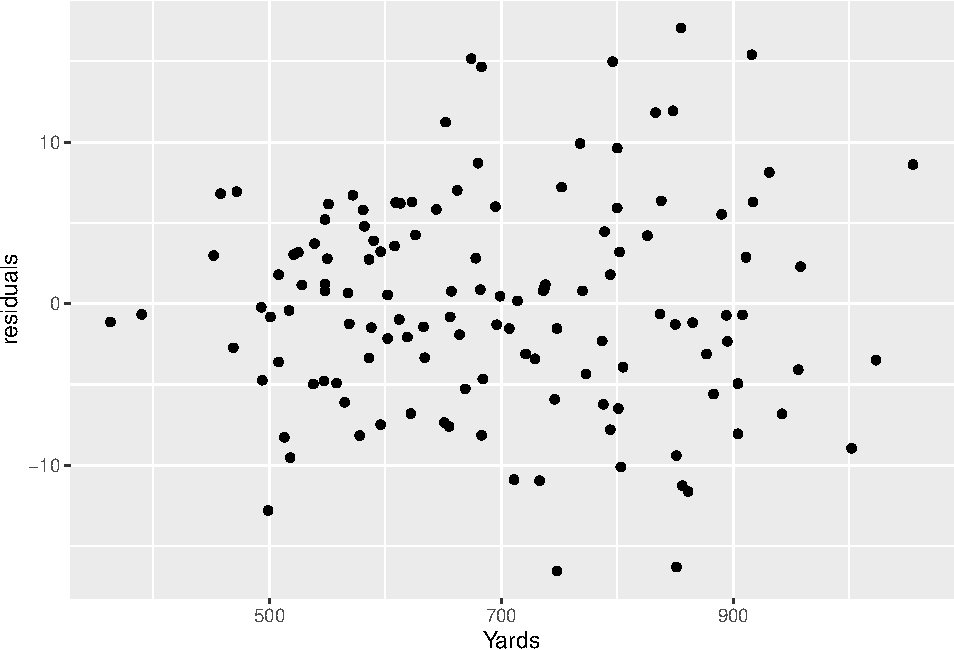
\includegraphics{SportsData_files/figure-latex/unnamed-chunk-90-1.pdf}

Well \ldots{} it actually says that a linear model is appropriate. Which an important lesson -- just because your residual plot says a linear model works here, that doesn't say your linear model is good. There are other measures for that, and you need to use them.

Here's the segment plot of residuals -- you'll see some really long lines. That's a bad sign.

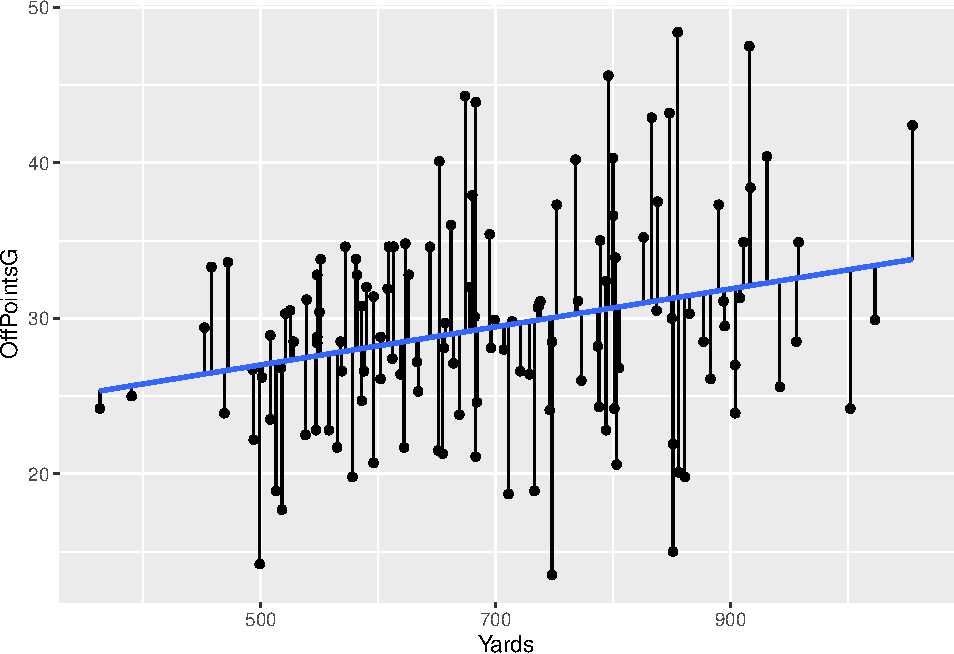
\includegraphics{SportsData_files/figure-latex/unnamed-chunk-91-1.pdf}

\hypertarget{z-scores}{%
\chapter{Z scores}\label{z-scores}}

Z scores are a handy way to standardize scores so you can compare things across groupings. In our case, we may want to compare teams by year, or era. We can use z scores to answer questions like who was the greatest X of all time, because a Z score can put them in context to their era.

We can also use z scores to ask how much better is team A from team B.

So let's use Nebraska basketball, which if you haven't been reading lately is at a bit of a crossroads.

A Z score is a measure of how far a number is from the population mean of that number. An easier way to say that -- how different is my grade from the average grade in the class. The formula for calculating a Z score is \texttt{(MyScore\ -\ AverageScore)/Standard\ Deviation\ of\ Scores}. The standard deviation is a number calculated to show the amount of variation in a set of data. In a normal distribution, 68 percent of all scores will be within 1 standard deviation, 95 percent will be within 2 and 99 within 3.

\hypertarget{calculating-a-z-score-in-r}{%
\section{Calculating a Z score in R}\label{calculating-a-z-score-in-r}}

\begin{Shaded}
\begin{Highlighting}[]
\KeywordTok{library}\NormalTok{(tidyverse)}
\end{Highlighting}
\end{Shaded}

Let's look at the current state of Nebraska basketball using the \href{https://unl.box.com/s/wnlh0u9low1yh56enion8zjmu8r7dc8p}{same logs data we've been using, but for this season so far}.

\begin{Shaded}
\begin{Highlighting}[]
\NormalTok{gamelogs <-}\StringTok{ }\KeywordTok{read_csv}\NormalTok{(}\StringTok{"data/logs20.csv"}\NormalTok{)}
\end{Highlighting}
\end{Shaded}

\begin{verbatim}
## Parsed with column specification:
## cols(
##   .default = col_double(),
##   Date = col_date(format = ""),
##   HomeAway = col_character(),
##   Opponent = col_character(),
##   W_L = col_character(),
##   Blank = col_logical(),
##   Team = col_character(),
##   Conference = col_character(),
##   season = col_character()
## )
\end{verbatim}

\begin{verbatim}
## See spec(...) for full column specifications.
\end{verbatim}

The first thing we need to do is select some fields we think represent team quality:

\begin{Shaded}
\begin{Highlighting}[]
\NormalTok{teamquality <-}\StringTok{ }\NormalTok{gamelogs }\OperatorTok\StringTok{ }
\StringTok{  }\KeywordTok{select}\NormalTok{(Conference, Team, TeamFGPCT, TeamTotalRebounds, OpponentFGPCT, OpponentTotalRebounds)}
\end{Highlighting}
\end{Shaded}

And since we have individual game data, we need to collapse this into one record for each team. We do that with \ldots{} group by.

\begin{Shaded}
\begin{Highlighting}[]
\NormalTok{teamtotals <-}\StringTok{ }\NormalTok{teamquality }\OperatorTok\StringTok{ }
\StringTok{  }\KeywordTok{group_by}\NormalTok{(Conference, Team) }\OperatorTok\StringTok{ }
\StringTok{  }\KeywordTok{summarise}\NormalTok{(}
    \DataTypeTok{FGAvg =} \KeywordTok{mean}\NormalTok{(TeamFGPCT), }
    \DataTypeTok{ReboundAvg =} \KeywordTok{mean}\NormalTok{(TeamTotalRebounds), }
    \DataTypeTok{OppFGAvg =} \KeywordTok{mean}\NormalTok{(OpponentFGPCT),}
    \DataTypeTok{OffRebAvg =} \KeywordTok{mean}\NormalTok{(OpponentTotalRebounds)}
\NormalTok{    )}
\end{Highlighting}
\end{Shaded}

To calculate a Z score in R, the easiest way is to use the scale function in base R. To use it, you use \texttt{scale(FieldName,\ center=TRUE,\ scale=TRUE)}. The center and scale indicate if you want to subtract from the mean and if you want to divide by the standard deviation, respectively. We do.

When we have multiple Z Scores, it's pretty standard practice to add them together into a composite score. That's what we're doing at the end here with \texttt{TotalZscore}. Note: We have to invert OppZscore and OppRebZScore by multiplying it by a negative 1 because the lower someone's opponent number is, the better.

\begin{Shaded}
\begin{Highlighting}[]
\NormalTok{teamzscore <-}\StringTok{ }\NormalTok{teamtotals }\OperatorTok\StringTok{ }
\StringTok{  }\KeywordTok{mutate}\NormalTok{(}
    \DataTypeTok{FGzscore =} \KeywordTok{as.numeric}\NormalTok{(}\KeywordTok{scale}\NormalTok{(FGAvg, }\DataTypeTok{center =} \OtherTok{TRUE}\NormalTok{, }\DataTypeTok{scale =} \OtherTok{TRUE}\NormalTok{)),}
    \DataTypeTok{RebZscore =} \KeywordTok{as.numeric}\NormalTok{(}\KeywordTok{scale}\NormalTok{(ReboundAvg, }\DataTypeTok{center =} \OtherTok{TRUE}\NormalTok{, }\DataTypeTok{scale =} \OtherTok{TRUE}\NormalTok{)),}
    \DataTypeTok{OppZscore =} \KeywordTok{as.numeric}\NormalTok{(}\KeywordTok{scale}\NormalTok{(OppFGAvg, }\DataTypeTok{center =} \OtherTok{TRUE}\NormalTok{, }\DataTypeTok{scale =} \OtherTok{TRUE}\NormalTok{)) }\OperatorTok{*}\StringTok{ }\DecValTok{-1}\NormalTok{,}
    \DataTypeTok{OppRebZScore =} \KeywordTok{as.numeric}\NormalTok{(}\KeywordTok{scale}\NormalTok{(OffRebAvg, }\DataTypeTok{center =} \OtherTok{TRUE}\NormalTok{, }\DataTypeTok{scale =} \OtherTok{TRUE}\NormalTok{)) }\OperatorTok{*}\StringTok{ }\DecValTok{-1}\NormalTok{,}
    \DataTypeTok{TotalZscore =}\NormalTok{ FGzscore }\OperatorTok{+}\StringTok{ }\NormalTok{RebZscore }\OperatorTok{+}\StringTok{ }\NormalTok{OppZscore }\OperatorTok{+}\StringTok{ }\NormalTok{OppRebZScore}
\NormalTok{  )  }
\end{Highlighting}
\end{Shaded}

So now we have a dataframe called \texttt{teamzscore} that has 353 basketball teams with Z scores. What does it look like?

\begin{Shaded}
\begin{Highlighting}[]
\KeywordTok{head}\NormalTok{(teamzscore)}
\end{Highlighting}
\end{Shaded}

\begin{verbatim}
## # A tibble: 6 x 11
## # Groups:   Conference [1]
##   Conference Team  FGAvg ReboundAvg OppFGAvg OffRebAvg FGzscore RebZscore
##   <chr>      <chr> <dbl>      <dbl>    <dbl>     <dbl>    <dbl>     <dbl>
## 1 A-10       Davi~ 0.454       31.1    0.437      30.4    0.505   -0.619 
## 2 A-10       Dayt~ 0.525       32.5    0.413      29.0    2.59     0.0352
## 3 A-10       Duqu~ 0.444       32.4    0.427      32.4    0.216   -0.0168
## 4 A-10       Ford~ 0.384       30.0    0.402      33.9   -1.53    -1.13  
## 5 A-10       Geor~ 0.424       33.8    0.440      30.5   -0.358    0.620 
## 6 A-10       Geor~ 0.422       30.5    0.452      32.7   -0.410   -0.904 
## # ... with 3 more variables: OppZscore <dbl>, OppRebZScore <dbl>,
## #   TotalZscore <dbl>
\end{verbatim}

A way to read this -- a team at zero is precisely average. The larger the positive number, the more exceptional they are. The larger the negative number, the more truly terrible they are.

So who are the best teams in the country?

\begin{Shaded}
\begin{Highlighting}[]
\NormalTok{teamzscore }\OperatorTok\StringTok{ }\KeywordTok{arrange}\NormalTok{(}\KeywordTok{desc}\NormalTok{(TotalZscore))}
\end{Highlighting}
\end{Shaded}

\begin{verbatim}
## # A tibble: 353 x 11
## # Groups:   Conference [32]
##    Conference Team  FGAvg ReboundAvg OppFGAvg OffRebAvg FGzscore RebZscore
##    <chr>      <chr> <dbl>      <dbl>    <dbl>     <dbl>    <dbl>     <dbl>
##  1 Big West   UC-I~ 0.473       36.6    0.390      27.1    1.60     2.23  
##  2 Big 12     Kans~ 0.482       35.9    0.378      29.0    2.36     1.13  
##  3 WCC        Gonz~ 0.517       37.4    0.424      28.2    1.73     1.90  
##  4 Southland  Step~ 0.490       34.2    0.427      26.6    1.76     1.05  
##  5 Big Ten    Mich~ 0.460       37.7    0.382      29.6    1.38     1.55  
##  6 OVC        Murr~ 0.477       35.3    0.401      29.2    1.31     1.36  
##  7 Summit     Sout~ 0.492       35.5    0.423      31.3    1.58     1.52  
##  8 A-10       Dayt~ 0.525       32.5    0.413      29.0    2.59     0.0352
##  9 A-10       Sain~ 0.457       37.4    0.403      30.5    0.598    2.21  
## 10 ACC        Loui~ 0.457       36.6    0.392      29.8    1.11     1.37  
## # ... with 343 more rows, and 3 more variables: OppZscore <dbl>,
## #   OppRebZScore <dbl>, TotalZscore <dbl>
\end{verbatim}

Don't sleep on the Anteaters come tournament time!

But closer to home, how is Nebraska doing.

\begin{Shaded}
\begin{Highlighting}[]
\NormalTok{teamzscore }\OperatorTok\StringTok{ }
\StringTok{  }\KeywordTok{filter}\NormalTok{(Conference }\OperatorTok{==}\StringTok{ "Big Ten"}\NormalTok{) }\OperatorTok\StringTok{ }
\StringTok{  }\KeywordTok{arrange}\NormalTok{(}\KeywordTok{desc}\NormalTok{(TotalZscore))}
\end{Highlighting}
\end{Shaded}

\begin{verbatim}
## # A tibble: 14 x 11
## # Groups:   Conference [1]
##    Conference Team  FGAvg ReboundAvg OppFGAvg OffRebAvg FGzscore RebZscore
##    <chr>      <chr> <dbl>      <dbl>    <dbl>     <dbl>    <dbl>     <dbl>
##  1 Big Ten    Mich~ 0.460       37.7    0.382      29.6    1.38      1.55 
##  2 Big Ten    Rutg~ 0.449       37      0.385      31.1    0.727     1.22 
##  3 Big Ten    Ohio~ 0.447       33.6    0.400      28.4    0.592    -0.393
##  4 Big Ten    Illi~ 0.444       36.1    0.418      29.1    0.439     0.779
##  5 Big Ten    Indi~ 0.445       35.1    0.419      29.4    0.480     0.306
##  6 Big Ten    Mary~ 0.419       36.1    0.401      31.9   -0.952     0.794
##  7 Big Ten    Mich~ 0.463       33.0    0.428      31.9    1.56     -0.682
##  8 Big Ten    Penn~ 0.432       35.6    0.411      34.2   -0.237     0.550
##  9 Big Ten    Minn~ 0.426       35.5    0.411      33     -0.560     0.520
## 10 Big Ten    Iowa~ 0.452       34.2    0.430      32.4    0.918    -0.104
## 11 Big Ten    Purd~ 0.418       33.8    0.410      29.3   -1.02     -0.271
## 12 Big Ten    Wisc~ 0.426       31.3    0.410      32.0   -0.587    -1.49 
## 13 Big Ten    Nort~ 0.417       30.5    0.422      34.8   -1.12     -1.84 
## 14 Big Ten    Nebr~ 0.408       32.4    0.453      42.2   -1.62     -0.947
## # ... with 3 more variables: OppZscore <dbl>, OppRebZScore <dbl>,
## #   TotalZscore <dbl>
\end{verbatim}

So, as we can see, with our composite Z Score, Nebraska is \ldots{} not good. Not good at all.

\hypertarget{intro-to-ggplot}{%
\chapter{Intro to ggplot}\label{intro-to-ggplot}}

With \texttt{ggplot2}, we dive into the world of programmatic data visualization. The \texttt{ggplot2} library implements something called the grammar of graphics. The main concepts are:

\begin{itemize}
\tightlist
\item
  aesthetics - which in this case means the data which we are going to plot
\item
  geometries - which means the shape the data is going to take
\item
  scales - which means any transformations we might make on the data
\item
  facets - which means how we might graph many elements of the same dataset in the same space
\item
  layers - which means how we might lay multiple geometries over top of each other to reveal new information.
\end{itemize}

Hadley Wickam, who is behind all of the libraries we have used in this course to date, wrote about his layered grammar of graphics in \href{http://byrneslab.net/classes/biol607/readings/wickham_layered-grammar.pdf}{this 2009 paper that is worth your time to read}.

Here are some \texttt{ggplot2} resources you'll want to keep handy:

\begin{itemize}
\tightlist
\item
  \href{http://ggplot2.tidyverse.org/reference/index.html}{The ggplot documentation}.
\item
  \href{http://www.cookbook-r.com/Graphs/}{The ggplot cookbook}
\end{itemize}

Let's dive in using data we've already seen before -- football attendance. This workflow will represent a clear picture of what your work in this class will be like for much of the rest of the semester. One way to think of this workflow is that your R Notebook is now your digital sketchbook, where you will try different types of visualizations to find ones that work. Then, you will export your work into a program like Illustrator to finish the work.

To begin, we'll import the \texttt{ggplot2} and \texttt{dplyr} libraries. We'll read in the data, then create a new dataframe that represents \href{https://unl.box.com/s/etqna5bfvf3b0gsnw0kcjjn1rxx9335s}{our attendance data}, similar to what we've done before.

\begin{Shaded}
\begin{Highlighting}[]
\KeywordTok{library}\NormalTok{(tidyverse)}
\end{Highlighting}
\end{Shaded}

\begin{Shaded}
\begin{Highlighting}[]
\NormalTok{attendance <-}\StringTok{ }\KeywordTok{read_csv}\NormalTok{(}\StringTok{'data/attendance.csv'}\NormalTok{)}
\end{Highlighting}
\end{Shaded}

\begin{verbatim}
## Parsed with column specification:
## cols(
##   Institution = col_character(),
##   Conference = col_character(),
##   `2013` = col_double(),
##   `2014` = col_double(),
##   `2015` = col_double(),
##   `2016` = col_double(),
##   `2017` = col_double(),
##   `2018` = col_double()
## )
\end{verbatim}

First, let's get a top 10 list by announced attendance this last season. We'll use the same tricks we used in the filtering assignment.

\begin{Shaded}
\begin{Highlighting}[]
\NormalTok{attendance }\OperatorTok\StringTok{ }
\StringTok{  }\KeywordTok{arrange}\NormalTok{(}\KeywordTok{desc}\NormalTok{(}\StringTok{`}\DataTypeTok{2018}\StringTok{`}\NormalTok{)) }\OperatorTok\StringTok{ }
\StringTok{  }\KeywordTok{top_n}\NormalTok{(}\DecValTok{10}\NormalTok{) }\OperatorTok\StringTok{ }
\StringTok{  }\KeywordTok{select}\NormalTok{(Institution, }\StringTok{`}\DataTypeTok{2018}\StringTok{`}\NormalTok{)}
\end{Highlighting}
\end{Shaded}

\begin{verbatim}
## Selecting by 2018
\end{verbatim}

\begin{verbatim}
## # A tibble: 10 x 2
##    Institution `2018`
##    <chr>        <dbl>
##  1 Michigan    775156
##  2 Penn St.    738396
##  3 Ohio St.    713630
##  4 Alabama     710931
##  5 LSU         705733
##  6 Texas A&M   698908
##  7 Tennessee   650887
##  8 Georgia     649222
##  9 Nebraska    623240
## 10 Oklahoma    607146
\end{verbatim}

That looks good, so let's save it to a new data frame and use that data frame instead going forward.

\begin{Shaded}
\begin{Highlighting}[]
\NormalTok{top10 <-}\StringTok{ }\NormalTok{attendance }\OperatorTok
\StringTok{  }\KeywordTok{arrange}\NormalTok{(}\KeywordTok{desc}\NormalTok{(}\StringTok{`}\DataTypeTok{2018}\StringTok{`}\NormalTok{)) }\OperatorTok\StringTok{ }
\StringTok{  }\KeywordTok{top_n}\NormalTok{(}\DecValTok{10}\NormalTok{) }\OperatorTok\StringTok{ }
\StringTok{  }\KeywordTok{select}\NormalTok{(Institution, }\StringTok{`}\DataTypeTok{2018}\StringTok{`}\NormalTok{)}
\end{Highlighting}
\end{Shaded}

\begin{verbatim}
## Selecting by 2018
\end{verbatim}

\hypertarget{the-bar-chart}{%
\section{The bar chart}\label{the-bar-chart}}

The easiest thing we can do is create a simple bar chart of our data. \textbf{Bar charts show magnitude. They invite you to compare how much more or less one thing is compared to others.}

We could, for instance, create a bar chart of the total attendance. To do that, we simply tell \texttt{ggplot2} what our dataset is, what element of the data we want to make the bar chart out of (which is the aesthetic), and the geometry type (which is the geom). It looks like this:

\texttt{ggplot(top10,\ aes(x=Institution))\ +\ geom\_bar()}

Note: attendance is our data, \texttt{aes} means aesthetics, \texttt{x=Institution} explicitly tells \texttt{ggplot2} that our x value -- our horizontal value -- is the Institution field from the data, and then we add on the \texttt{geom\_bar()} as the geometry. And what do we get when we run that?

\begin{Shaded}
\begin{Highlighting}[]
\KeywordTok{ggplot}\NormalTok{(top10, }\KeywordTok{aes}\NormalTok{(}\DataTypeTok{x=}\NormalTok{Institution)) }\OperatorTok{+}\StringTok{ }\KeywordTok{geom_bar}\NormalTok{()}
\end{Highlighting}
\end{Shaded}

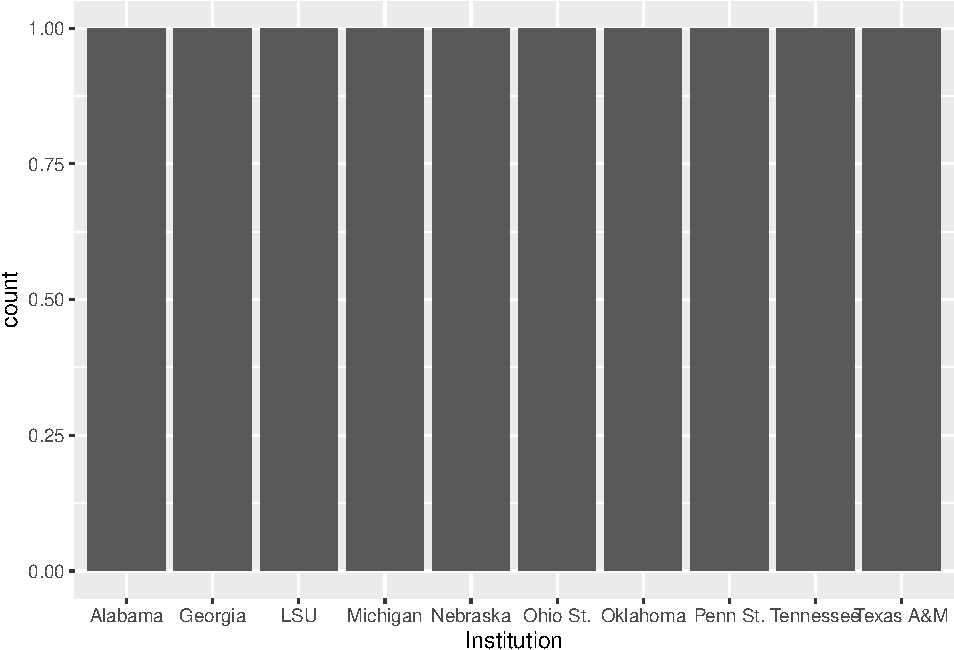
\includegraphics{SportsData_files/figure-latex/unnamed-chunk-104-1.pdf}

We get \ldots{} weirdness. We expected to see bars of different sizes, but we get all with a count of 1. What gives? Well, this is the default behavior. What we have here is something called a histogram, where \texttt{ggplot2} helpfully counted up the number of times the Institution appears and counted them up. Since we only have one record per Institution, the count is always 1. How do we fix this? By adding \texttt{weight} to our aesthetic.

\begin{Shaded}
\begin{Highlighting}[]
\KeywordTok{ggplot}\NormalTok{(top10, }\KeywordTok{aes}\NormalTok{(}\DataTypeTok{x=}\NormalTok{Institution, }\DataTypeTok{weight=}\StringTok{`}\DataTypeTok{2018}\StringTok{`}\NormalTok{)) }\OperatorTok{+}\StringTok{ }
\StringTok{  }\KeywordTok{geom_bar}\NormalTok{()}
\end{Highlighting}
\end{Shaded}

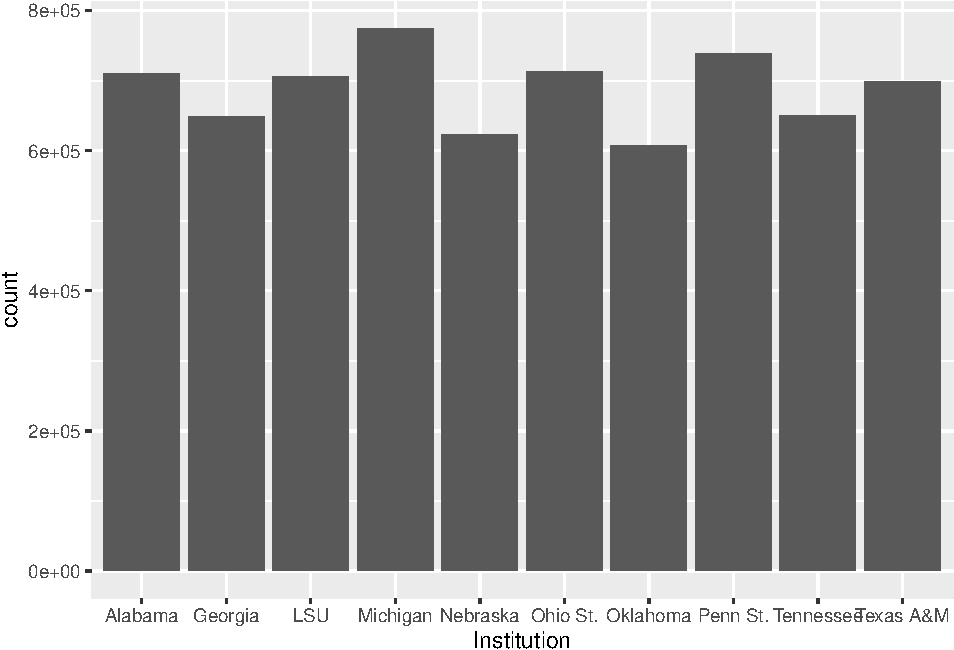
\includegraphics{SportsData_files/figure-latex/unnamed-chunk-105-1.pdf}

Closer. But \ldots{} what order is that in? And what happened to our count numbers on the left? Why are they in scientific notation?

Let's deal with the ordering first. \texttt{ggplot2}'s default behavior is to sort the data by the x axis variable. So it's in alphabetical order. To change that, we have to \texttt{reorder} it. With \texttt{reorder}, we first have to tell \texttt{ggplot} what we are reordering, and then we have to tell it HOW we are reordering it. So it's reorder(FIELD, SORTFIELD).

\begin{Shaded}
\begin{Highlighting}[]
\KeywordTok{ggplot}\NormalTok{(top10, }\KeywordTok{aes}\NormalTok{(}\DataTypeTok{x=}\KeywordTok{reorder}\NormalTok{(Institution, }\StringTok{`}\DataTypeTok{2018}\StringTok{`}\NormalTok{), }\DataTypeTok{weight=}\StringTok{`}\DataTypeTok{2018}\StringTok{`}\NormalTok{)) }\OperatorTok{+}\StringTok{ }\KeywordTok{geom_bar}\NormalTok{()}
\end{Highlighting}
\end{Shaded}

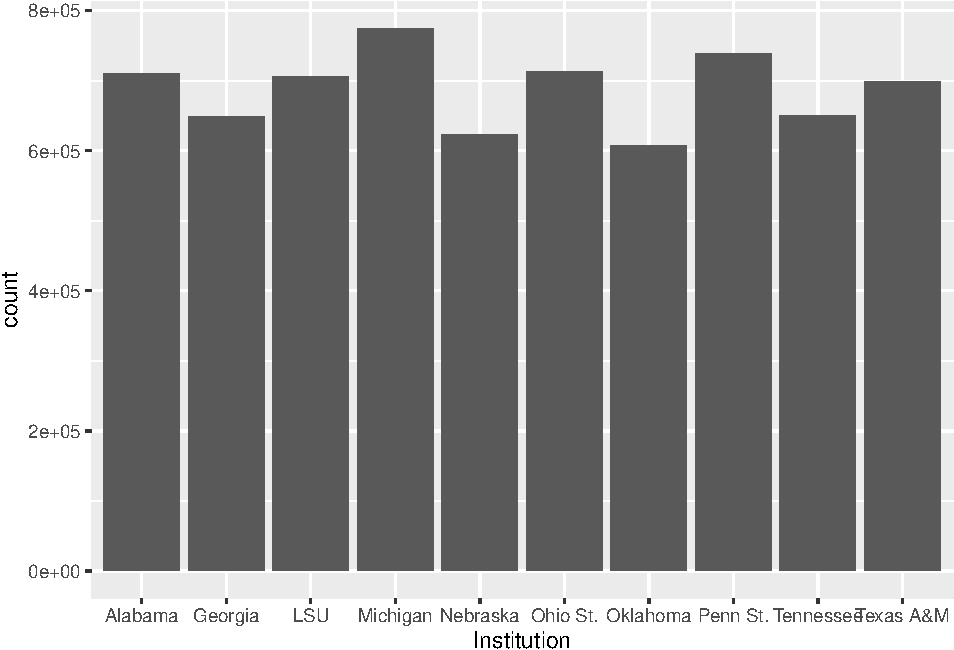
\includegraphics{SportsData_files/figure-latex/unnamed-chunk-106-1.pdf}

Better. We can argue about if the right order is smallest to largest or largest to smallest. But this gets us close. By the way, to sort it largest to smallest, put a negative sign in front of the sort field.

\begin{Shaded}
\begin{Highlighting}[]
\KeywordTok{ggplot}\NormalTok{(top10, }\KeywordTok{aes}\NormalTok{(}\DataTypeTok{x=}\KeywordTok{reorder}\NormalTok{(Institution, }\OperatorTok{-}\StringTok{`}\DataTypeTok{2018}\StringTok{`}\NormalTok{), }\DataTypeTok{weight=}\StringTok{`}\DataTypeTok{2018}\StringTok{`}\NormalTok{)) }\OperatorTok{+}\StringTok{ }\KeywordTok{geom_bar}\NormalTok{()}
\end{Highlighting}
\end{Shaded}

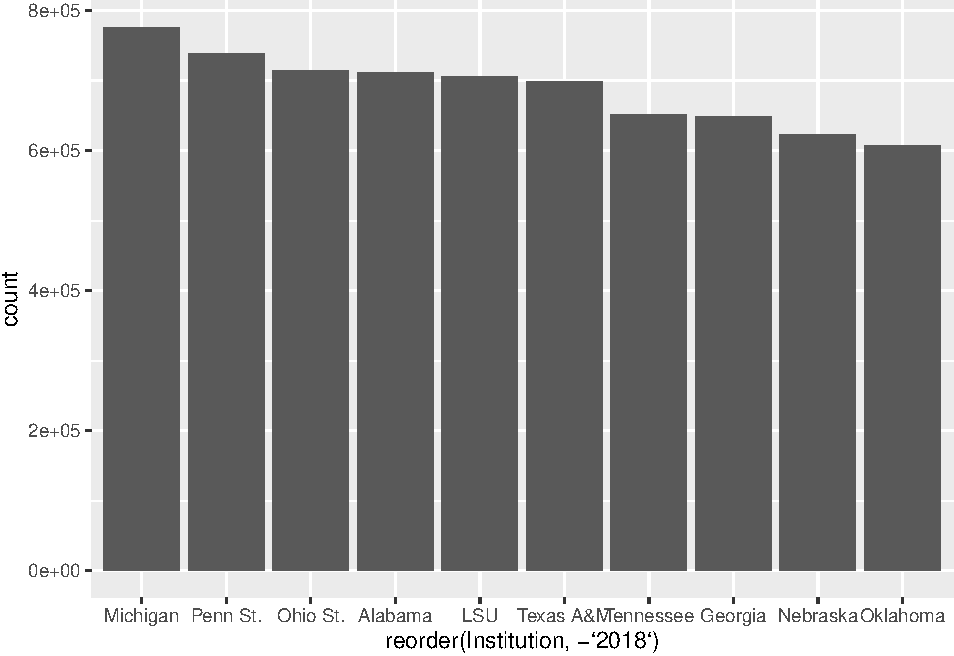
\includegraphics{SportsData_files/figure-latex/unnamed-chunk-107-1.pdf}

\hypertarget{scales}{%
\section{Scales}\label{scales}}

To fix the axis labels, we need try one of the other main elements of the \texttt{ggplot2} library, which is transform a scale. More often that not, that means doing something like putting it on a logarithmic scale or some other kind of transformation. In this case, we're just changing how it's represented. The default in \texttt{ggplot2} for large values is to express them as scientific notation. Rarely ever is that useful in our line of work. So we have to transform them into human readable numbers.

The easiest way to do this is to use a library called \texttt{scales} and it's already installed.

\begin{Shaded}
\begin{Highlighting}[]
\KeywordTok{library}\NormalTok{(scales)}
\end{Highlighting}
\end{Shaded}

To alter the scale, we add a piece to our plot with \texttt{+} and we tell it which scale is getting altered and what kind of data it is. In our case, our Y axis is what is needing to be altered, and it's continuous data (meaning it can be any number between x and y, vs discrete data which are categorical). So we need to add \texttt{scale\_y\_continuous} and the information we want to pass it is to alter the labels with a function called \texttt{comma}.

\begin{Shaded}
\begin{Highlighting}[]
\KeywordTok{ggplot}\NormalTok{(top10, }\KeywordTok{aes}\NormalTok{(}\DataTypeTok{x=}\KeywordTok{reorder}\NormalTok{(Institution, }\OperatorTok{-}\StringTok{`}\DataTypeTok{2018}\StringTok{`}\NormalTok{), }\DataTypeTok{weight=}\StringTok{`}\DataTypeTok{2018}\StringTok{`}\NormalTok{)) }\OperatorTok{+}\StringTok{ }
\StringTok{  }\KeywordTok{geom_bar}\NormalTok{() }\OperatorTok{+}\StringTok{ }
\StringTok{  }\KeywordTok{scale_y_continuous}\NormalTok{(}\DataTypeTok{labels=}\NormalTok{comma)}
\end{Highlighting}
\end{Shaded}

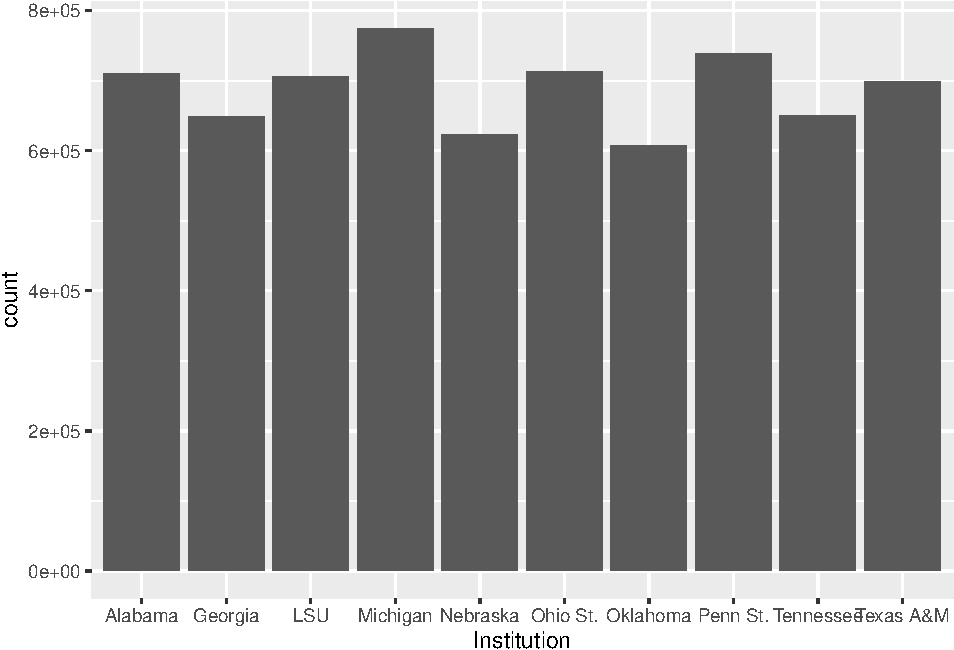
\includegraphics{SportsData_files/figure-latex/unnamed-chunk-109-1.pdf}

Better.

\hypertarget{styling}{%
\section{Styling}\label{styling}}

We are going to spend a lot more time on styling, but let's add some simple labels to this with a new bit called \texttt{labs} which is short for labels.

\begin{Shaded}
\begin{Highlighting}[]
\KeywordTok{ggplot}\NormalTok{(top10, }\KeywordTok{aes}\NormalTok{(}\DataTypeTok{x=}\KeywordTok{reorder}\NormalTok{(Institution, }\OperatorTok{-}\StringTok{`}\DataTypeTok{2018}\StringTok{`}\NormalTok{), }\DataTypeTok{weight=}\StringTok{`}\DataTypeTok{2018}\StringTok{`}\NormalTok{)) }\OperatorTok{+}\StringTok{ }
\StringTok{  }\KeywordTok{geom_bar}\NormalTok{() }\OperatorTok{+}\StringTok{ }
\StringTok{  }\KeywordTok{scale_y_continuous}\NormalTok{(}\DataTypeTok{labels=}\NormalTok{comma) }\OperatorTok{+}\StringTok{ }
\StringTok{  }\KeywordTok{labs}\NormalTok{(}\DataTypeTok{title=}\StringTok{"Top 10 Football Programs By Attendance"}\NormalTok{, }\DataTypeTok{x=}\StringTok{"School"}\NormalTok{, }\DataTypeTok{y=}\StringTok{"Attendance"}\NormalTok{)}
\end{Highlighting}
\end{Shaded}

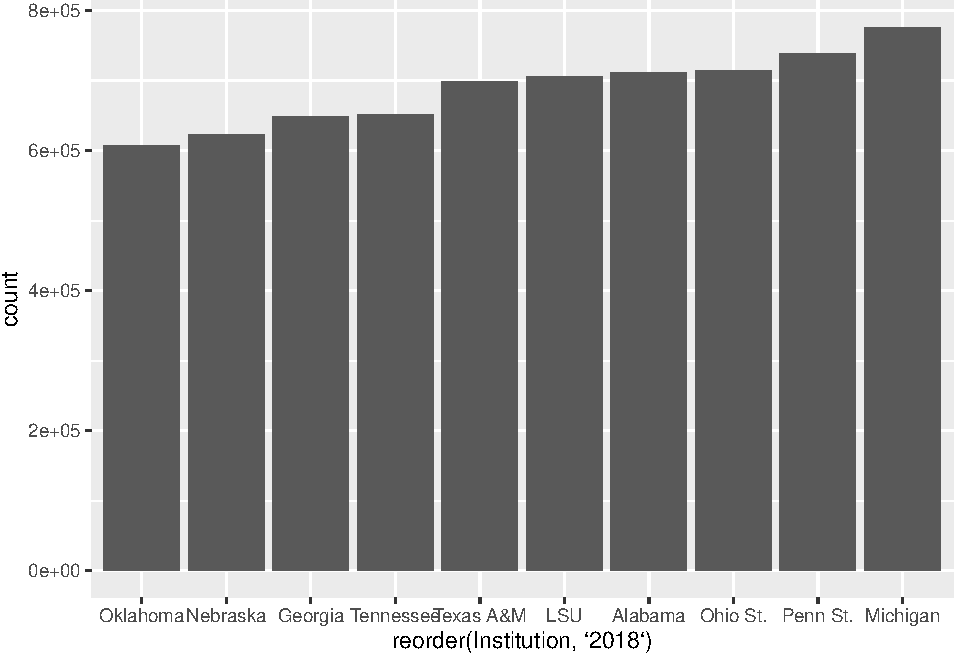
\includegraphics{SportsData_files/figure-latex/unnamed-chunk-110-1.pdf}

The library has lots and lots of ways to alter the styling -- we can programmatically control nearly every part of the look and feel of the chart. One simple way is to apply themes in the library already. We do that the same way we've done other things -- we add them. Here's the light theme.

\begin{Shaded}
\begin{Highlighting}[]
\KeywordTok{ggplot}\NormalTok{(top10, }\KeywordTok{aes}\NormalTok{(}\DataTypeTok{x=}\KeywordTok{reorder}\NormalTok{(Institution, }\OperatorTok{-}\StringTok{`}\DataTypeTok{2018}\StringTok{`}\NormalTok{), }\DataTypeTok{weight=}\StringTok{`}\DataTypeTok{2018}\StringTok{`}\NormalTok{)) }\OperatorTok{+}\StringTok{ }
\StringTok{  }\KeywordTok{geom_bar}\NormalTok{() }\OperatorTok{+}\StringTok{ }
\StringTok{  }\KeywordTok{scale_y_continuous}\NormalTok{(}\DataTypeTok{labels=}\NormalTok{comma) }\OperatorTok{+}\StringTok{ }
\StringTok{  }\KeywordTok{labs}\NormalTok{(}\DataTypeTok{title=}\StringTok{"Top 10 Football Programs By Attendance"}\NormalTok{, }\DataTypeTok{x=}\StringTok{"School"}\NormalTok{, }\DataTypeTok{y=}\StringTok{"Attendance"}\NormalTok{) }\OperatorTok{+}\StringTok{ }
\StringTok{  }\KeywordTok{theme_light}\NormalTok{()}
\end{Highlighting}
\end{Shaded}

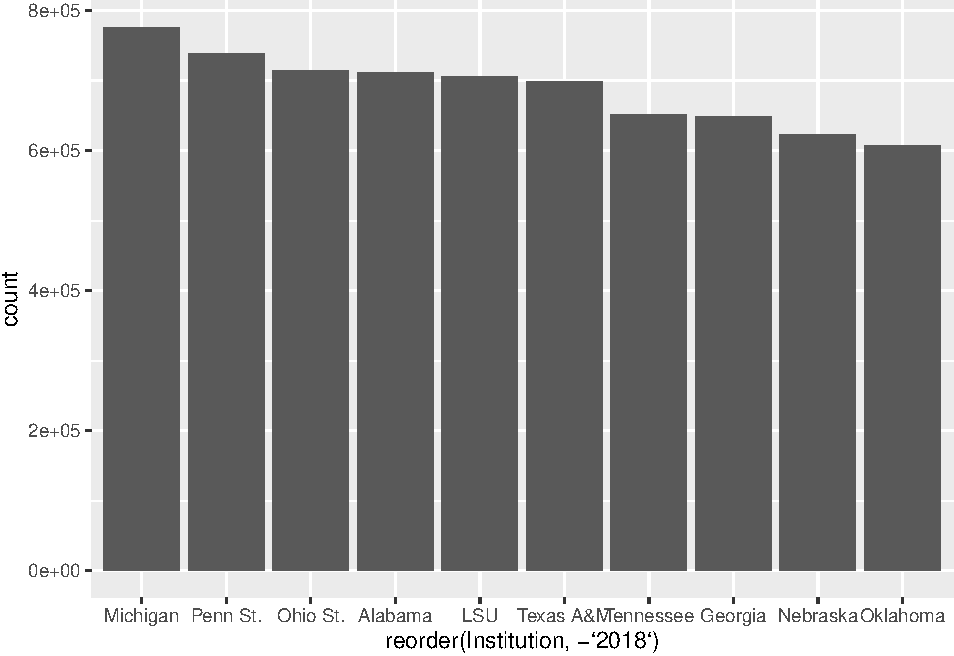
\includegraphics{SportsData_files/figure-latex/unnamed-chunk-111-1.pdf}

Or the minimal theme:

\begin{Shaded}
\begin{Highlighting}[]
\KeywordTok{ggplot}\NormalTok{(top10, }\KeywordTok{aes}\NormalTok{(}\DataTypeTok{x=}\KeywordTok{reorder}\NormalTok{(Institution, }\OperatorTok{-}\StringTok{`}\DataTypeTok{2018}\StringTok{`}\NormalTok{), }\DataTypeTok{weight=}\StringTok{`}\DataTypeTok{2018}\StringTok{`}\NormalTok{)) }\OperatorTok{+}\StringTok{ }
\StringTok{  }\KeywordTok{geom_bar}\NormalTok{() }\OperatorTok{+}\StringTok{ }
\StringTok{  }\KeywordTok{scale_y_continuous}\NormalTok{(}\DataTypeTok{labels=}\NormalTok{comma) }\OperatorTok{+}\StringTok{ }
\StringTok{  }\KeywordTok{labs}\NormalTok{(}\DataTypeTok{title=}\StringTok{"Top 10 Football Programs By Attendance"}\NormalTok{, }\DataTypeTok{x=}\StringTok{"School"}\NormalTok{, }\DataTypeTok{y=}\StringTok{"Attendance"}\NormalTok{) }\OperatorTok{+}\StringTok{ }
\StringTok{  }\KeywordTok{theme_minimal}\NormalTok{()}
\end{Highlighting}
\end{Shaded}

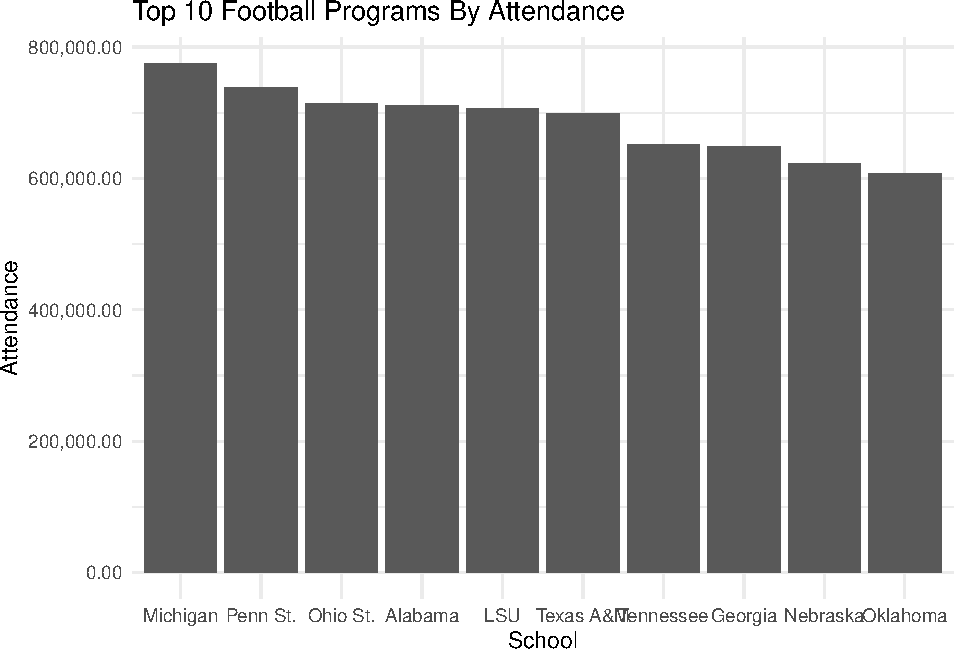
\includegraphics{SportsData_files/figure-latex/unnamed-chunk-112-1.pdf}

Later on, we'll write our own themes. For now, the built in ones will get us closer to something that looks good.

\hypertarget{one-last-trick-coord-flip}{%
\section{One last trick: coord flip}\label{one-last-trick-coord-flip}}

Sometimes, we don't want vertical bars. Maybe we think this would look better horizontal. How do we do that? By adding \texttt{coord\_flip()} to our code. It does what it says -- it inverts the coordinates of the figures.

\begin{Shaded}
\begin{Highlighting}[]
\KeywordTok{ggplot}\NormalTok{(top10, }\KeywordTok{aes}\NormalTok{(}\DataTypeTok{x=}\KeywordTok{reorder}\NormalTok{(Institution, }\OperatorTok{-}\StringTok{`}\DataTypeTok{2018}\StringTok{`}\NormalTok{), }\DataTypeTok{weight=}\StringTok{`}\DataTypeTok{2018}\StringTok{`}\NormalTok{)) }\OperatorTok{+}\StringTok{ }
\StringTok{  }\KeywordTok{geom_bar}\NormalTok{() }\OperatorTok{+}\StringTok{ }
\StringTok{  }\KeywordTok{scale_y_continuous}\NormalTok{(}\DataTypeTok{labels=}\NormalTok{comma) }\OperatorTok{+}\StringTok{ }
\StringTok{  }\KeywordTok{labs}\NormalTok{(}\DataTypeTok{title=}\StringTok{"Top 10 Football Programs By Attendance"}\NormalTok{, }\DataTypeTok{x=}\StringTok{"School"}\NormalTok{, }\DataTypeTok{y=}\StringTok{"Attendance"}\NormalTok{) }\OperatorTok{+}\StringTok{ }
\StringTok{  }\KeywordTok{theme_minimal}\NormalTok{() }\OperatorTok{+}\StringTok{ }
\StringTok{  }\KeywordTok{coord_flip}\NormalTok{()}
\end{Highlighting}
\end{Shaded}

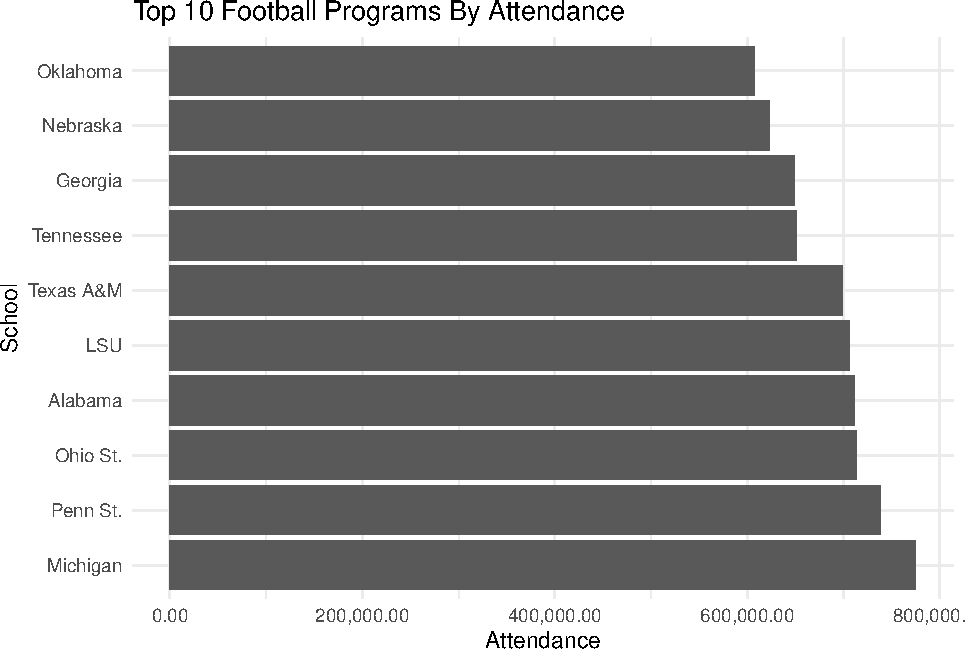
\includegraphics{SportsData_files/figure-latex/unnamed-chunk-113-1.pdf}

\hypertarget{stacked-bar-charts}{%
\chapter{Stacked bar charts}\label{stacked-bar-charts}}

One of the elements of data visualization excellence is \textbf{inviting comparison}. Often that comes in showing \textbf{what proportion a thing is in relation to the whole thing}. With bar charts, we're showing magnitude of the whole thing. If we have information about the parts of the whole, \textbf{we can stack them on top of each other to compare them, showing both the whole and the components}. And it's a simple change to what we've already done.

\begin{Shaded}
\begin{Highlighting}[]
\KeywordTok{library}\NormalTok{(tidyverse)}
\end{Highlighting}
\end{Shaded}

We're going to use a dataset of graduation rates by gender by school in the NCAA. \href{https://unl.box.com/s/3nw1eokvs9zfdjyzvjaj3xdq01rm8sym}{You can get it here}.

\begin{Shaded}
\begin{Highlighting}[]
\NormalTok{grads <-}\StringTok{ }\KeywordTok{read_csv}\NormalTok{(}\StringTok{'data/grads.csv'}\NormalTok{)}
\end{Highlighting}
\end{Shaded}

\begin{verbatim}
## Parsed with column specification:
## cols(
##   `Institution name` = col_character(),
##   `Primary Conference in Actual Year` = col_character(),
##   `Cohort year` = col_double(),
##   Gender = col_character(),
##   `Number of completers` = col_double(),
##   Total = col_double()
## )
\end{verbatim}

What we have here is the name of the school, the conference, the cohort of when they started school, the gender, the number of that gender that graduated and the total number of graduates in that cohort.

Let's pretend for a moment we're looking at the graduation rates of men and women in the Big 10 Conference and we want to chart that. First, let's work on our data. We need to filter the ``Big Ten Conference'' school, and we want the latest year, which is 2009. So we'll create a dataframe called \texttt{BIG09} and populate it.

\begin{Shaded}
\begin{Highlighting}[]
\NormalTok{BIG09 <-}\StringTok{ }\NormalTok{grads }\OperatorTok\StringTok{ }\KeywordTok{filter}\NormalTok{(}\StringTok{`}\DataTypeTok{Primary Conference in Actual Year}\StringTok{`}\OperatorTok{==}\StringTok{"Big Ten Conference"}\NormalTok{) }\OperatorTok\StringTok{ }\KeywordTok{filter}\NormalTok{(}\StringTok{`}\DataTypeTok{Cohort year}\StringTok{`} \OperatorTok{==}\StringTok{ }\DecValTok{2009}\NormalTok{)}
\end{Highlighting}
\end{Shaded}

Reminder: \texttt{head()} will give you a quick look at what your data looks like, but \textbf{it will only show you the first six rows}.

\begin{Shaded}
\begin{Highlighting}[]
\KeywordTok{head}\NormalTok{(BIG09)}
\end{Highlighting}
\end{Shaded}

\begin{verbatim}
## # A tibble: 6 x 6
##   `Institution nam~ `Primary Confer~ `Cohort year` Gender `Number of comp~ Total
##   <chr>             <chr>                    <dbl> <chr>             <dbl> <dbl>
## 1 University of Il~ Big Ten Confere~          2009 Men                2973  5940
## 2 University of Il~ Big Ten Confere~          2009 Women              2967  5940
## 3 Northwestern Uni~ Big Ten Confere~          2009 Men                 963  1974
## 4 Northwestern Uni~ Big Ten Confere~          2009 Women              1011  1974
## 5 Indiana Universi~ Big Ten Confere~          2009 Men                2667  5626
## 6 Indiana Universi~ Big Ten Confere~          2009 Women              2959  5626
\end{verbatim}

Building on what we learned in the last chapter, we know we can turn this into a bar chart with an x value, a weight and a geom\_bar. What're going to add is a \texttt{fill}. The \texttt{fill} will stack bars on each other based on which element it is. In this case, we can fill the bar by Gender, which means it will stack the number of male graduates on top of the number of female graduates and we can see how they compare.

\begin{Shaded}
\begin{Highlighting}[]
\KeywordTok{ggplot}\NormalTok{(BIG09, }\KeywordTok{aes}\NormalTok{(}\DataTypeTok{x=}\KeywordTok{reorder}\NormalTok{(}\StringTok{`}\DataTypeTok{Institution name}\StringTok{`}\NormalTok{, }\OperatorTok{-}\NormalTok{Total), }\DataTypeTok{weight=}\StringTok{`}\DataTypeTok{Number of completers}\StringTok{`}\NormalTok{, }\DataTypeTok{fill=}\NormalTok{Gender)) }\OperatorTok{+}\StringTok{ }\KeywordTok{geom_bar}\NormalTok{() }\OperatorTok{+}\StringTok{ }\KeywordTok{coord_flip}\NormalTok{()}
\end{Highlighting}
\end{Shaded}

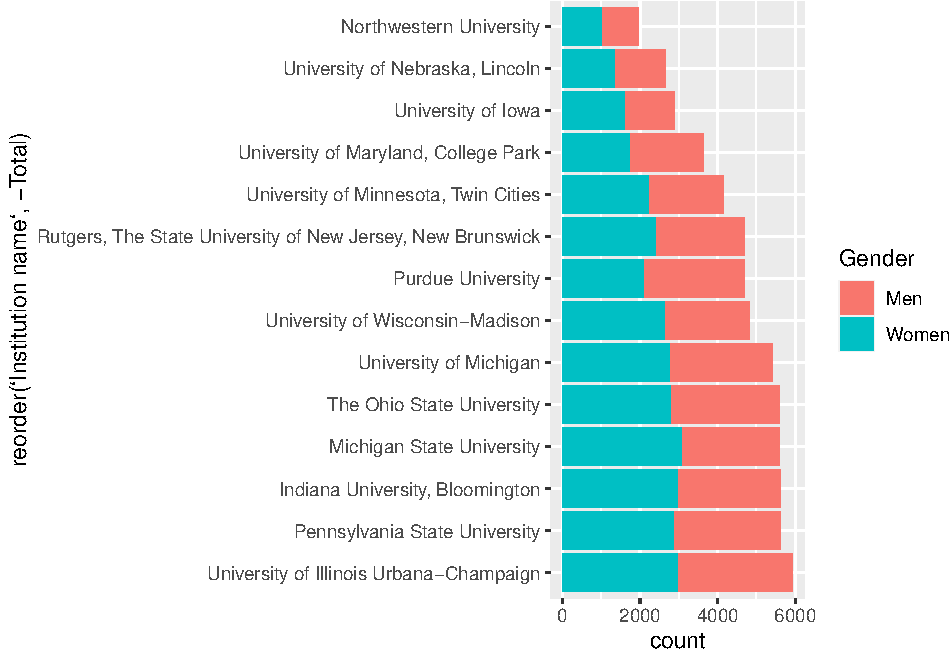
\includegraphics{SportsData_files/figure-latex/unnamed-chunk-118-1.pdf}

What's the problem with this chart?

Let me ask a different question -- which schools have larger differences in male and female graduation rates? Can you compare Illnois to Northwestern? Not really. We've charted the total numbers. We need the percentage of the whole.

\begin{quote}
\textbf{YOUR TURN}: Using what you know -- hint: mutate -- how could you chart this using percents of the whole instead of counts?
\end{quote}

\hypertarget{waffle-charts}{%
\chapter{Waffle charts}\label{waffle-charts}}

Pie charts are the devil. They should be an instant F in any data visualization class. I'll give you an example of why.

What's the racial breakdown of journalism majors at UNL?

Here it is in a pie chart:

\begin{Shaded}
\begin{Highlighting}[]
\KeywordTok{library}\NormalTok{(tidyverse)}

\NormalTok{enrollment <-}\StringTok{ }\KeywordTok{read.csv}\NormalTok{(}\StringTok{"~/Box/Courses/JOUR407-Data-Visualization/Data/collegeenrollment.csv"}\NormalTok{)}

\NormalTok{jour <-}\StringTok{ }\KeywordTok{filter}\NormalTok{(enrollment, MajorName }\OperatorTok{==}\StringTok{ "Journalism"}\NormalTok{)}

\NormalTok{jdf <-}\StringTok{ }\NormalTok{jour }\OperatorTok\StringTok{ }
\KeywordTok{group_by}\NormalTok{(Race) }\OperatorTok
\KeywordTok{summarise}\NormalTok{(}
       \DataTypeTok{total=}\KeywordTok{sum}\NormalTok{(Count)) }\OperatorTok
\KeywordTok{select}\NormalTok{(Race, total) }\OperatorTok\StringTok{ }
\KeywordTok{filter}\NormalTok{(total }\OperatorTok{!=}\StringTok{ }\DecValTok{0}\NormalTok{)}

\KeywordTok{ggplot}\NormalTok{(jdf, }\KeywordTok{aes}\NormalTok{(}\DataTypeTok{x=}\StringTok{""}\NormalTok{, }\DataTypeTok{y=}\NormalTok{total, }\DataTypeTok{fill=}\NormalTok{Race)) }\OperatorTok{+}\StringTok{ }\KeywordTok{geom_bar}\NormalTok{(}\DataTypeTok{width =} \DecValTok{1}\NormalTok{, }\DataTypeTok{stat =} \StringTok{"identity"}\NormalTok{) }\OperatorTok{+}\StringTok{ }\KeywordTok{coord_polar}\NormalTok{(}\StringTok{"y"}\NormalTok{, }\DataTypeTok{start=}\DecValTok{0}\NormalTok{)}
\end{Highlighting}
\end{Shaded}

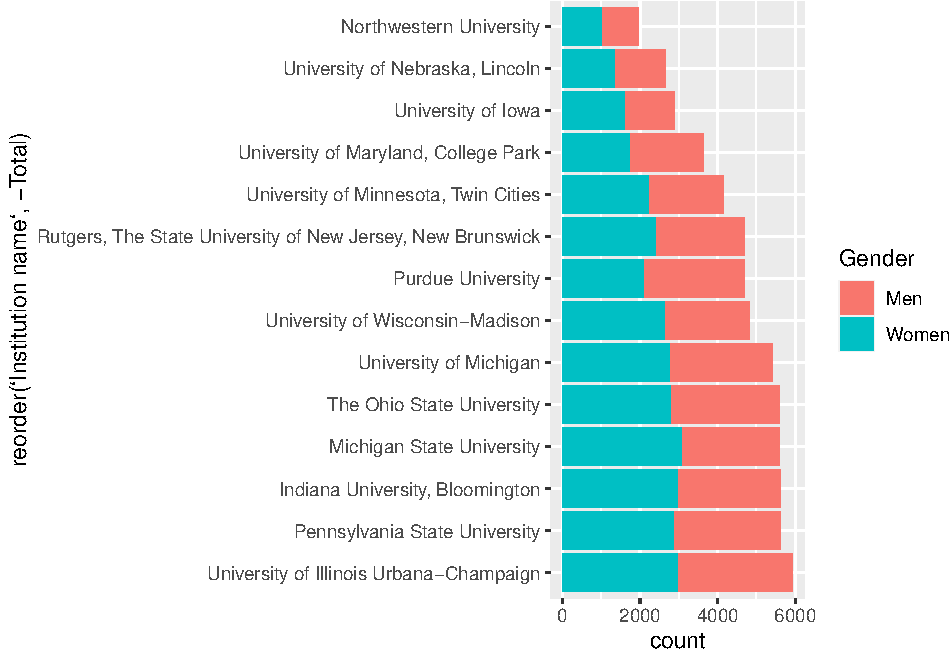
\includegraphics{SportsData_files/figure-latex/unnamed-chunk-119-1.pdf}

You can see, it's pretty white. But \ldots{} what about beyond that? How carefully can you evaluate angles and area?

Not well.

So let's introduce a better way: The Waffle Chart. Some call it a square pie chart. I personally hate that. Waffles it is.

\textbf{A waffle chart is designed to show you parts of the whole -- proportionality}. How many yards on offense come from rushing or passing. How many singles, doubles, triples and home runs make up a teams hits. How many shots a basketball team takes are two pointers versus three pointers.

First, install the library in the console:

\texttt{install.packages(\textquotesingle{}waffle\textquotesingle{})}

Now load it:

\begin{Shaded}
\begin{Highlighting}[]
\KeywordTok{library}\NormalTok{(waffle)}
\end{Highlighting}
\end{Shaded}

Let's look at the debacle that was Nebraska vs.~Ohio State this fall in Football. \href{https://www.espn.com/college-football/matchup?gameId=401112241}{Here's the box score}, which we'll use for this walkthrough.

The easiest way to do waffle charts is to make vectors of your data and plug them in. To make a vector, we use the \texttt{c} or concatenate function, something we've done before.

So let's look at offense. Rushing vs passing.

\begin{Shaded}
\begin{Highlighting}[]
\NormalTok{nu <-}\StringTok{ }\KeywordTok{c}\NormalTok{(}\StringTok{"Rushing"}\NormalTok{=}\DecValTok{184}\NormalTok{, }\StringTok{"Passing"}\NormalTok{=}\DecValTok{47}\NormalTok{)}
\NormalTok{oh <-}\StringTok{ }\KeywordTok{c}\NormalTok{(}\StringTok{"Rushing"}\NormalTok{=}\DecValTok{368}\NormalTok{, }\StringTok{"Passing"}\NormalTok{=}\DecValTok{212}\NormalTok{)}
\end{Highlighting}
\end{Shaded}

So what does the breakdown of the night look like?

The waffle library can break this down in a way that's easier on the eyes than a pie chart. We call the library, add the data, specify the number of rows, give it a title and an x value label, and to clean up a quirk of the library, we've got to specify colors.

\begin{Shaded}
\begin{Highlighting}[]
\KeywordTok{waffle}\NormalTok{(nu, }\DataTypeTok{rows =} \DecValTok{10}\NormalTok{, }\DataTypeTok{title=}\StringTok{"Nebraska's offense"}\NormalTok{, }\DataTypeTok{xlab=}\StringTok{"1 square = 1 yard"}\NormalTok{, }\DataTypeTok{colors =} \KeywordTok{c}\NormalTok{(}\StringTok{"black"}\NormalTok{, }\StringTok{"red"}\NormalTok{))}
\end{Highlighting}
\end{Shaded}

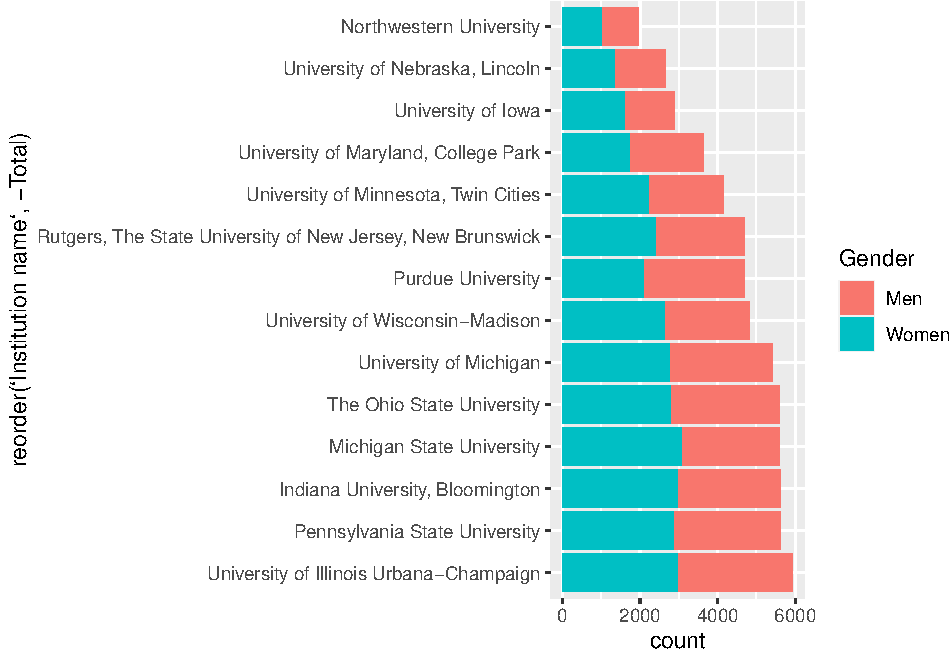
\includegraphics{SportsData_files/figure-latex/unnamed-chunk-122-1.pdf}

Or, we could make this two teams in the same chart.

\begin{Shaded}
\begin{Highlighting}[]
\NormalTok{passing <-}\StringTok{ }\KeywordTok{c}\NormalTok{(}\StringTok{"Nebraska"}\NormalTok{=}\DecValTok{47}\NormalTok{, }\StringTok{"Ohio State"}\NormalTok{=}\DecValTok{212}\NormalTok{)}
\end{Highlighting}
\end{Shaded}

\begin{Shaded}
\begin{Highlighting}[]
\KeywordTok{waffle}\NormalTok{(passing, }\DataTypeTok{rows =} \DecValTok{10}\NormalTok{, }\DataTypeTok{title=}\StringTok{"Nebraska vs Ohio State: passing"}\NormalTok{, }\DataTypeTok{xlab=}\StringTok{"1 square = 1 yard"}\NormalTok{, }\DataTypeTok{colors =} \KeywordTok{c}\NormalTok{(}\StringTok{"red"}\NormalTok{, }\StringTok{"black"}\NormalTok{))}
\end{Highlighting}
\end{Shaded}

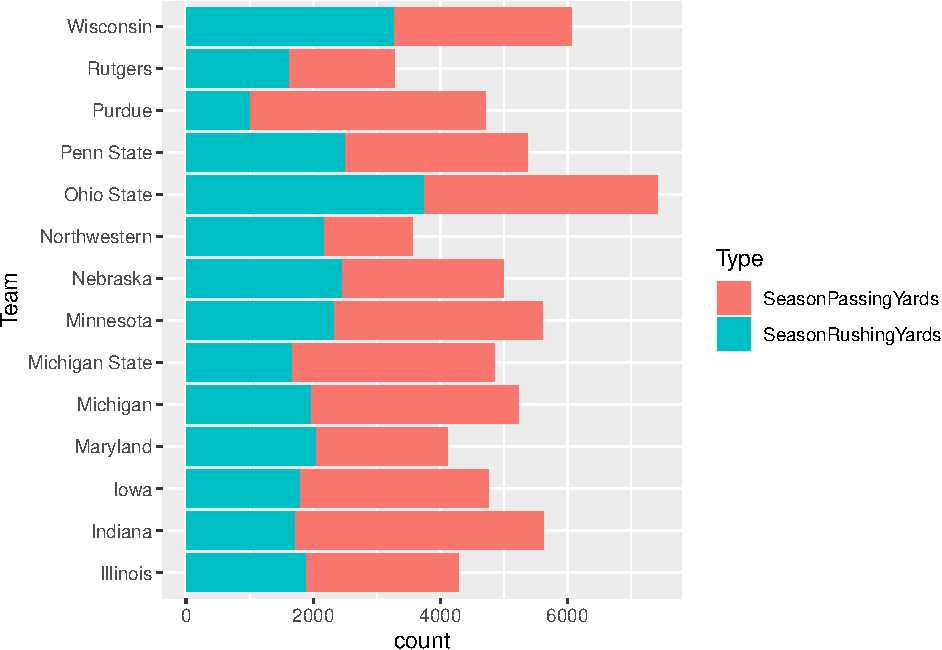
\includegraphics{SportsData_files/figure-latex/unnamed-chunk-124-1.pdf}

\hypertarget{waffle-irons}{%
\section{Waffle Irons}\label{waffle-irons}}

So what does it look like if we compare the two teams using the two vectors in the same chart? To do that -- and I am not making this up -- you have to create a waffle iron. Get it? Waffle charts? Iron?

\begin{Shaded}
\begin{Highlighting}[]
\KeywordTok{iron}\NormalTok{(}
 \KeywordTok{waffle}\NormalTok{(nu, }\DataTypeTok{rows =} \DecValTok{10}\NormalTok{, }\DataTypeTok{title=}\StringTok{"Nebraska's offense"}\NormalTok{, }\DataTypeTok{xlab=}\StringTok{"1 square = 1 yard"}\NormalTok{, }\DataTypeTok{colors =} \KeywordTok{c}\NormalTok{(}\StringTok{"black"}\NormalTok{, }\StringTok{"red"}\NormalTok{)),}
 \KeywordTok{waffle}\NormalTok{(oh, }\DataTypeTok{rows =} \DecValTok{10}\NormalTok{, }\DataTypeTok{title=}\StringTok{"Ohio State's offense"}\NormalTok{, }\DataTypeTok{xlab=}\StringTok{"1 square = 1 yard"}\NormalTok{, }\DataTypeTok{colors =} \KeywordTok{c}\NormalTok{(}\StringTok{"black"}\NormalTok{, }\StringTok{"red"}\NormalTok{))}
\NormalTok{)}
\end{Highlighting}
\end{Shaded}

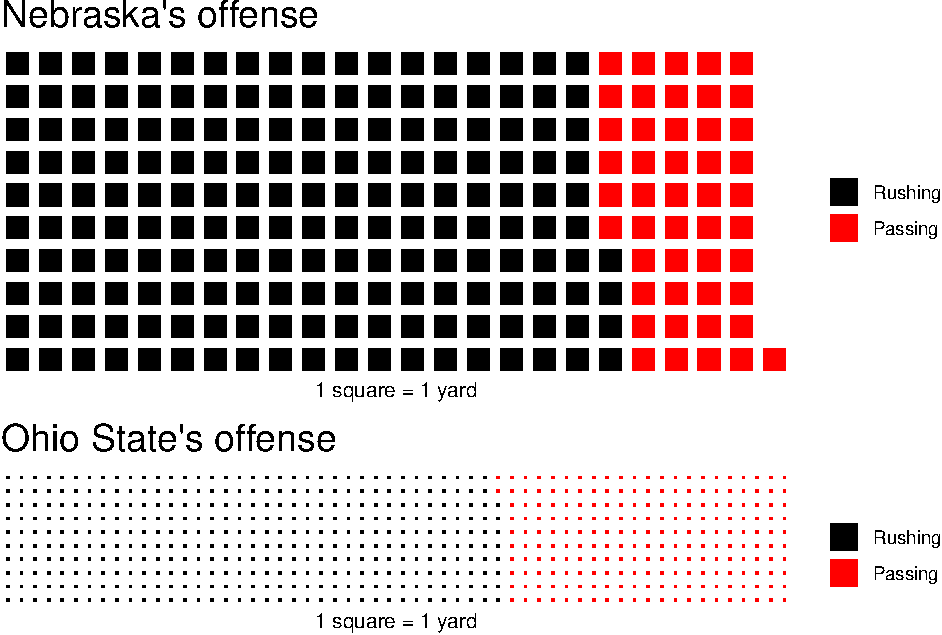
\includegraphics{SportsData_files/figure-latex/unnamed-chunk-125-1.pdf}

What do you notice about this chart? Notice how the squares aren't the same size? Well, Ohio State outgained Nebraska by a long way. So the squares aren't the same size because the numbers aren't the same. We can fix that by adding an unnamed padding number so the number of shots add up to the same thing. Let's make the total for everyone be 580, Ohio State's total yards of offense. So to do that, we need to add a padding of 349 to Nebraska. REMEMBER: Don't name it or it'll show up in the legend.

\begin{Shaded}
\begin{Highlighting}[]
\NormalTok{nu <-}\StringTok{ }\KeywordTok{c}\NormalTok{(}\StringTok{"Rushing"}\NormalTok{=}\DecValTok{184}\NormalTok{, }\StringTok{"Passing"}\NormalTok{=}\DecValTok{47}\NormalTok{, }\DecValTok{349}\NormalTok{)}
\NormalTok{oh <-}\StringTok{ }\KeywordTok{c}\NormalTok{(}\StringTok{"Rushing"}\NormalTok{=}\DecValTok{368}\NormalTok{, }\StringTok{"Passing"}\NormalTok{=}\DecValTok{212}\NormalTok{, }\DecValTok{0}\NormalTok{)}
\end{Highlighting}
\end{Shaded}

Now, in our waffle iron, if we don't give that padding a color, we'll get an error. So we need to make it white. Which, given our white background, means it will disappear.

\begin{Shaded}
\begin{Highlighting}[]
\KeywordTok{iron}\NormalTok{(}
 \KeywordTok{waffle}\NormalTok{(nu, }\DataTypeTok{rows =} \DecValTok{10}\NormalTok{, }\DataTypeTok{title=}\StringTok{"Nebraska's offense"}\NormalTok{, }\DataTypeTok{xlab=}\StringTok{"1 square = 1 yard"}\NormalTok{, }\DataTypeTok{colors =} \KeywordTok{c}\NormalTok{(}\StringTok{"black"}\NormalTok{, }\StringTok{"red"}\NormalTok{, }\StringTok{"white"}\NormalTok{)),}
 \KeywordTok{waffle}\NormalTok{(oh, }\DataTypeTok{rows =} \DecValTok{10}\NormalTok{, }\DataTypeTok{title=}\StringTok{"Ohio State's offense"}\NormalTok{, }\DataTypeTok{xlab=}\StringTok{"1 square = 1 yard"}\NormalTok{, }\DataTypeTok{colors =} \KeywordTok{c}\NormalTok{(}\StringTok{"black"}\NormalTok{, }\StringTok{"red"}\NormalTok{, }\StringTok{"white"}\NormalTok{))}
\NormalTok{)}
\end{Highlighting}
\end{Shaded}

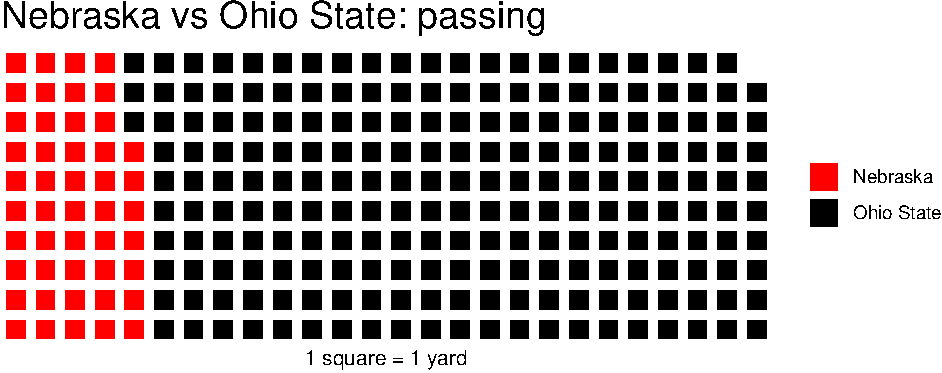
\includegraphics{SportsData_files/figure-latex/unnamed-chunk-127-1.pdf}

One last thing we can do is change the 1 square = 1 yard bit -- which makes the squares really small in this case -- by dividing our vector. Remember what you learned in Swirl about math on vectors?

\begin{Shaded}
\begin{Highlighting}[]
\KeywordTok{iron}\NormalTok{(}
 \KeywordTok{waffle}\NormalTok{(nu}\OperatorTok{/}\DecValTok{2}\NormalTok{, }\DataTypeTok{rows =} \DecValTok{10}\NormalTok{, }\DataTypeTok{title=}\StringTok{"Nebraska's offense"}\NormalTok{, }\DataTypeTok{xlab=}\StringTok{"1 square = 2 yards"}\NormalTok{, }\DataTypeTok{colors =} \KeywordTok{c}\NormalTok{(}\StringTok{"black"}\NormalTok{, }\StringTok{"red"}\NormalTok{, }\StringTok{"white"}\NormalTok{)),}
 \KeywordTok{waffle}\NormalTok{(oh}\OperatorTok{/}\DecValTok{2}\NormalTok{, }\DataTypeTok{rows =} \DecValTok{10}\NormalTok{, }\DataTypeTok{title=}\StringTok{"Ohio State's offense"}\NormalTok{, }\DataTypeTok{xlab=}\StringTok{"1 square = 2 yards"}\NormalTok{, }\DataTypeTok{colors =} \KeywordTok{c}\NormalTok{(}\StringTok{"black"}\NormalTok{, }\StringTok{"red"}\NormalTok{, }\StringTok{"white"}\NormalTok{))}
\NormalTok{)}
\end{Highlighting}
\end{Shaded}

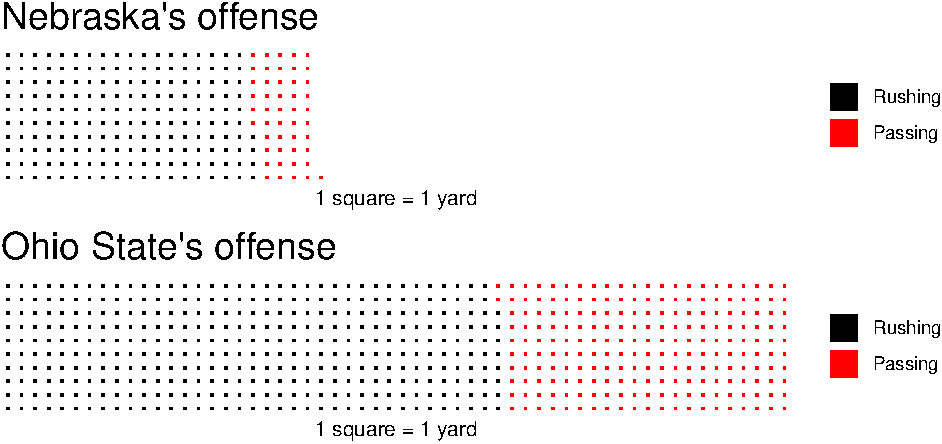
\includegraphics{SportsData_files/figure-latex/unnamed-chunk-128-1.pdf}

News flash: Ohio State crushed Nebraska.

\hypertarget{line-charts}{%
\chapter{Line charts}\label{line-charts}}

So far, we've talked about bar charts -- stacked or otherwise -- are good for showing relative size of a thing compared to another thing. Stacked Bars and Waffle charts are good at showing proportions of a whole.

\textbf{Line charts are good for showing change over time.}

Let's look at how we can answer this question: Why was Nebraska terrible at basketball last season?

Let's start getting all that we need. We can use the tidyverse shortcut.

\begin{Shaded}
\begin{Highlighting}[]
\KeywordTok{library}\NormalTok{(tidyverse)}
\end{Highlighting}
\end{Shaded}

Now we'll \href{https://unl.box.com/s/a8m91bro10t89watsyo13yjegb1fy009}{import the data you need}. Mine looks like this:

\begin{Shaded}
\begin{Highlighting}[]
\NormalTok{logs <-}\StringTok{ }\KeywordTok{read_csv}\NormalTok{(}\StringTok{"data/logs19.csv"}\NormalTok{)}
\end{Highlighting}
\end{Shaded}

\begin{verbatim}
## Warning: Missing column names filled in: 'X1' [1]
\end{verbatim}

\begin{verbatim}
## Parsed with column specification:
## cols(
##   .default = col_double(),
##   Date = col_date(format = ""),
##   HomeAway = col_character(),
##   Opponent = col_character(),
##   W_L = col_character(),
##   Blank = col_logical(),
##   Team = col_character(),
##   Conference = col_character(),
##   season = col_character()
## )
\end{verbatim}

\begin{verbatim}
## See spec(...) for full column specifications.
\end{verbatim}

This data has every game from every team in it, so we need to use filtering to limit it, because we just want to look at Nebraska. If you don't remember, flip back to chapter 5.

\begin{Shaded}
\begin{Highlighting}[]
\NormalTok{nu <-}\StringTok{ }\NormalTok{logs }\OperatorTok\StringTok{ }\KeywordTok{filter}\NormalTok{(Team }\OperatorTok{==}\StringTok{ "Nebraska Cornhuskers"}\NormalTok{)}
\end{Highlighting}
\end{Shaded}

Because this data has just Nebraska data in it, the dates are formatted correctly, and the data is long data (instead of wide), we have what we need to make line charts.

Line charts, unlike bar charts, do have a y-axis. So in our ggplot step, we have to define what our x and y axes are. In this case, the x axis is our Date -- the most common x axis in line charts is going to be a date of some variety -- and y in this case is up to us. We've seen from previous walkthroughs that how well a team shoots the ball has a lot to do with how well a team does in a season, so let's chart that.

\begin{Shaded}
\begin{Highlighting}[]
\KeywordTok{ggplot}\NormalTok{(nu, }\KeywordTok{aes}\NormalTok{(}\DataTypeTok{x=}\NormalTok{Date, }\DataTypeTok{y=}\NormalTok{TeamFGPCT)) }\OperatorTok{+}\StringTok{ }\KeywordTok{geom_line}\NormalTok{()}
\end{Highlighting}
\end{Shaded}

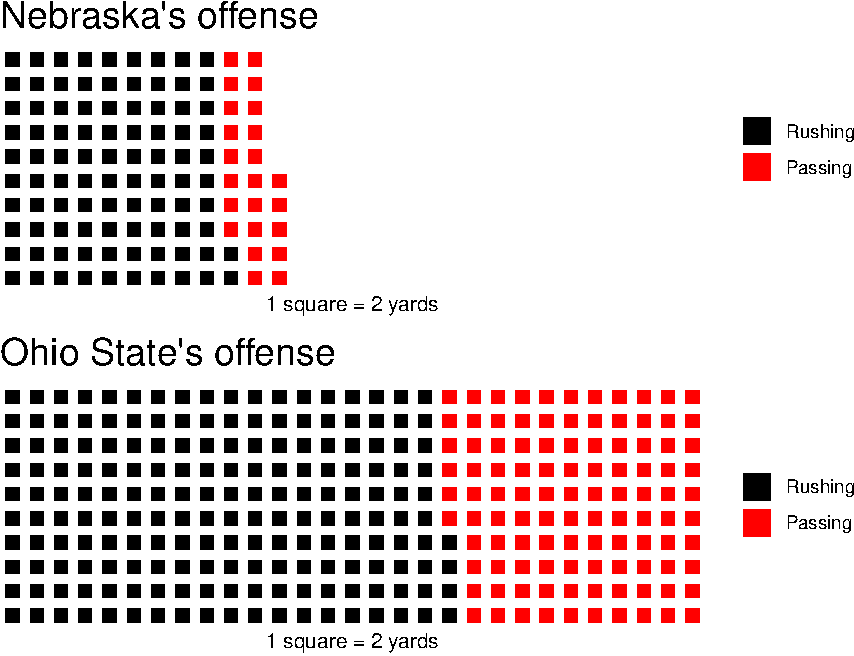
\includegraphics{SportsData_files/figure-latex/unnamed-chunk-132-1.pdf}

See a problem here? Note the Y axis doesn't start with zero. That makes this look worse than it is (and that February swoon is pretty bad). To make the axis what you want, you can use \texttt{scale\_x\_continuous} or \texttt{scale\_y\_continuous} and pass in a list with the bottom and top value you want. You do that like this:

\begin{Shaded}
\begin{Highlighting}[]
\KeywordTok{ggplot}\NormalTok{(nu, }\KeywordTok{aes}\NormalTok{(}\DataTypeTok{x=}\NormalTok{Date, }\DataTypeTok{y=}\NormalTok{TeamFGPCT)) }\OperatorTok{+}\StringTok{ }\KeywordTok{geom_line}\NormalTok{() }\OperatorTok{+}\StringTok{ }\KeywordTok{scale_y_continuous}\NormalTok{(}\DataTypeTok{limits =} \KeywordTok{c}\NormalTok{(}\DecValTok{0}\NormalTok{, }\FloatTok{.6}\NormalTok{))}
\end{Highlighting}
\end{Shaded}

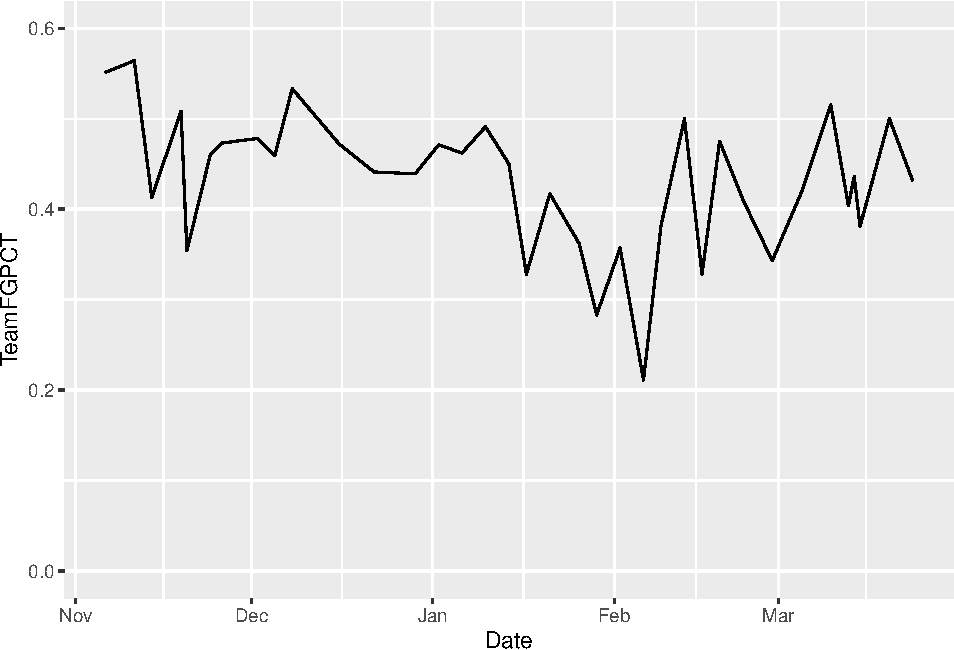
\includegraphics{SportsData_files/figure-latex/unnamed-chunk-133-1.pdf}

Note also that our X axis labels are automated. It knows it's a date and it just labels it by month.

\hypertarget{this-is-too-simple.}{%
\section{This is too simple.}\label{this-is-too-simple.}}

With datasets, we want to invite comparison. So let's answer the question visually. Let's put two lines on the same chart. How does Nebraska compare to Michigan State and Purdue, the eventual regular season co-champions?

\begin{Shaded}
\begin{Highlighting}[]
\NormalTok{msu <-}\StringTok{ }\NormalTok{logs }\OperatorTok\StringTok{ }\KeywordTok{filter}\NormalTok{(Team }\OperatorTok{==}\StringTok{ "Michigan State Spartans"}\NormalTok{)}
\end{Highlighting}
\end{Shaded}

In this case, because we have two different datasets, we're going to put everything in the geom instead of the ggplot step. We also have to explicitly state what dataset we're using by saying \texttt{data=} in the geom step.

First, let's chart Nebraska. Read carefully. First we set the data. Then we set our aesthetic. Unlike bars, we need an X and a Y variable. In this case, our X is the date of the game, Y is the thing we want the lines to move with. In this case, the Team Field Goal Percentage -- TeamFGPCT.

\begin{Shaded}
\begin{Highlighting}[]
\KeywordTok{ggplot}\NormalTok{() }\OperatorTok{+}\StringTok{ }\KeywordTok{geom_line}\NormalTok{(}\DataTypeTok{data=}\NormalTok{nu, }\KeywordTok{aes}\NormalTok{(}\DataTypeTok{x=}\NormalTok{Date, }\DataTypeTok{y=}\NormalTok{TeamFGPCT), }\DataTypeTok{color=}\StringTok{"red"}\NormalTok{)}
\end{Highlighting}
\end{Shaded}

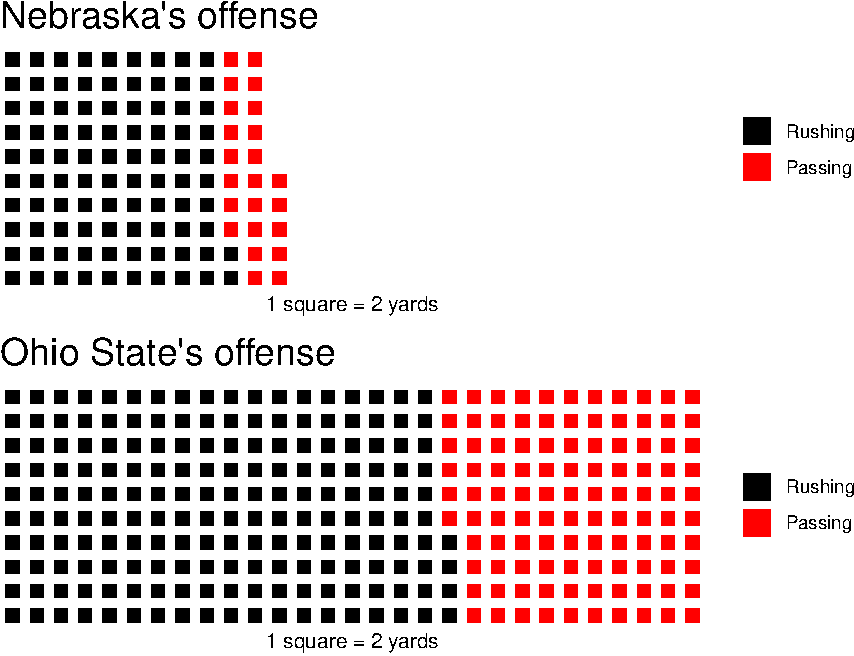
\includegraphics{SportsData_files/figure-latex/unnamed-chunk-135-1.pdf}

Now, by using +, we can add Michigan State to it. REMEMBER COPY AND PASTE IS A THING. Nothing changes except what data you are using.

\begin{Shaded}
\begin{Highlighting}[]
\KeywordTok{ggplot}\NormalTok{() }\OperatorTok{+}\StringTok{ }\KeywordTok{geom_line}\NormalTok{(}\DataTypeTok{data=}\NormalTok{nu, }\KeywordTok{aes}\NormalTok{(}\DataTypeTok{x=}\NormalTok{Date, }\DataTypeTok{y=}\NormalTok{TeamFGPCT), }\DataTypeTok{color=}\StringTok{"red"}\NormalTok{) }\OperatorTok{+}\StringTok{ }\KeywordTok{geom_line}\NormalTok{(}\DataTypeTok{data=}\NormalTok{msu, }\KeywordTok{aes}\NormalTok{(}\DataTypeTok{x=}\NormalTok{Date, }\DataTypeTok{y=}\NormalTok{TeamFGPCT), }\DataTypeTok{color=}\StringTok{"green"}\NormalTok{)}
\end{Highlighting}
\end{Shaded}

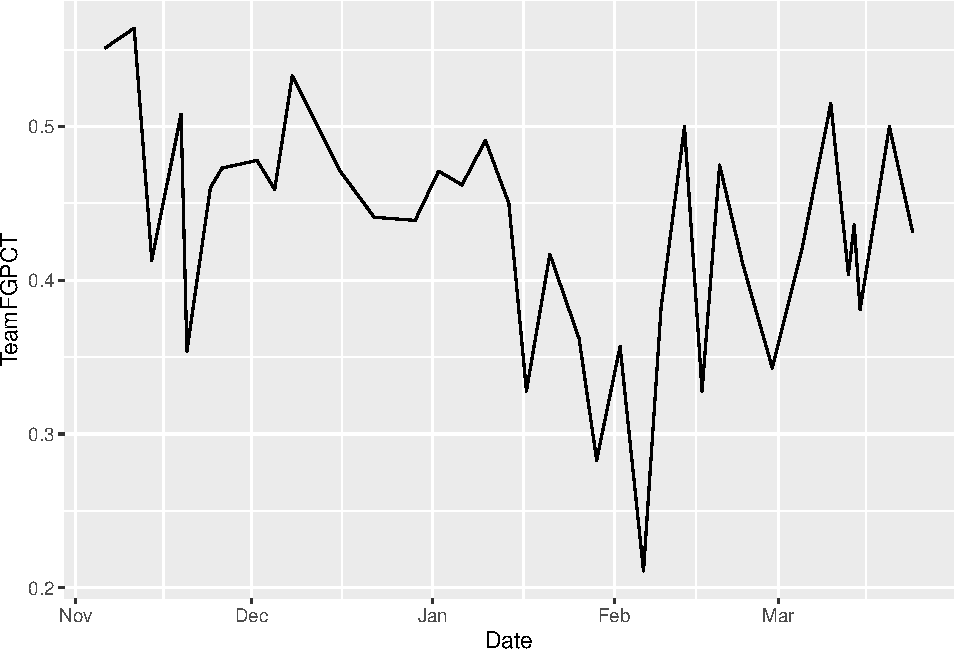
\includegraphics{SportsData_files/figure-latex/unnamed-chunk-136-1.pdf}

Let's flatten our lines out by zeroing the Y axis.

\begin{Shaded}
\begin{Highlighting}[]
\KeywordTok{ggplot}\NormalTok{() }\OperatorTok{+}\StringTok{ }\KeywordTok{geom_line}\NormalTok{(}\DataTypeTok{data=}\NormalTok{nu, }\KeywordTok{aes}\NormalTok{(}\DataTypeTok{x=}\NormalTok{Date, }\DataTypeTok{y=}\NormalTok{TeamFGPCT), }\DataTypeTok{color=}\StringTok{"red"}\NormalTok{) }\OperatorTok{+}\StringTok{ }\KeywordTok{geom_line}\NormalTok{(}\DataTypeTok{data=}\NormalTok{msu, }\KeywordTok{aes}\NormalTok{(}\DataTypeTok{x=}\NormalTok{Date, }\DataTypeTok{y=}\NormalTok{TeamFGPCT), }\DataTypeTok{color=}\StringTok{"green"}\NormalTok{) }\OperatorTok{+}\StringTok{ }\KeywordTok{scale_y_continuous}\NormalTok{(}\DataTypeTok{limits =} \KeywordTok{c}\NormalTok{(}\DecValTok{0}\NormalTok{, }\FloatTok{.65}\NormalTok{))}
\end{Highlighting}
\end{Shaded}

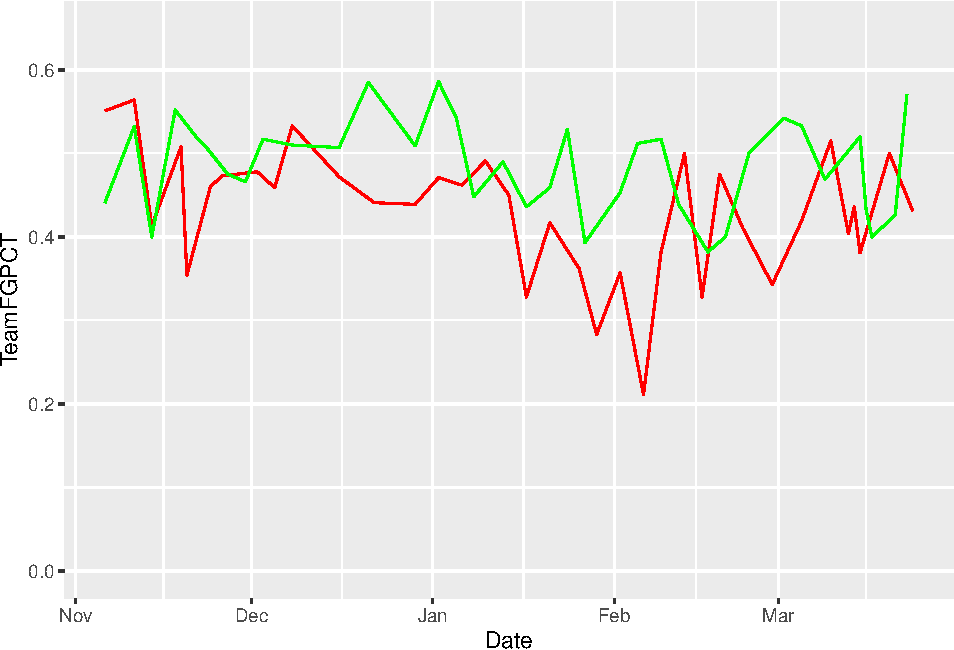
\includegraphics{SportsData_files/figure-latex/unnamed-chunk-137-1.pdf}

So visually speaking, the difference between Nebraska and Michigan State's season is that Michigan State stayed mostly on an even keel, and Nebraska went on a two month swoon.

\hypertarget{but-what-if-i-wanted-to-add-a-lot-of-lines.}{%
\section{But what if I wanted to add a lot of lines.}\label{but-what-if-i-wanted-to-add-a-lot-of-lines.}}

Fine. How about all Power Five Schools? This data for example purposes. You don't have to do it.

\begin{Shaded}
\begin{Highlighting}[]
\NormalTok{powerfive <-}\StringTok{ }\KeywordTok{c}\NormalTok{(}\StringTok{"SEC"}\NormalTok{, }\StringTok{"Big Ten"}\NormalTok{, }\StringTok{"Pac-12"}\NormalTok{, }\StringTok{"Big 12"}\NormalTok{, }\StringTok{"ACC"}\NormalTok{)}

\NormalTok{p5conf <-}\StringTok{ }\NormalTok{logs }\OperatorTok\StringTok{ }\KeywordTok{filter}\NormalTok{(Conference }\OperatorTok\StringTok{ }\NormalTok{powerfive)}
\end{Highlighting}
\end{Shaded}

I can keep layering on layers all day if I want. And if my dataset has more than one team in it, I need to use the \texttt{group} command. And, the layering comes in order -- so if you're going to layer a bunch of lines with a smaller group of lines, you want the bunch on the bottom. So to do that, your code stacks from the bottom. The first geom in the code gets rendered first. The second gets layered on top of that. The third gets layered on that and so on.

\begin{Shaded}
\begin{Highlighting}[]
\KeywordTok{ggplot}\NormalTok{() }\OperatorTok{+}\StringTok{ }\KeywordTok{geom_line}\NormalTok{(}\DataTypeTok{data=}\NormalTok{p5conf, }\KeywordTok{aes}\NormalTok{(}\DataTypeTok{x=}\NormalTok{Date, }\DataTypeTok{y=}\NormalTok{TeamFGPCT, }\DataTypeTok{group=}\NormalTok{Team), }\DataTypeTok{color=}\StringTok{"grey"}\NormalTok{) }\OperatorTok{+}\StringTok{ }\KeywordTok{geom_line}\NormalTok{(}\DataTypeTok{data=}\NormalTok{nu, }\KeywordTok{aes}\NormalTok{(}\DataTypeTok{x=}\NormalTok{Date, }\DataTypeTok{y=}\NormalTok{TeamFGPCT), }\DataTypeTok{color=}\StringTok{"red"}\NormalTok{) }\OperatorTok{+}\StringTok{ }\KeywordTok{geom_line}\NormalTok{(}\DataTypeTok{data=}\NormalTok{msu, }\KeywordTok{aes}\NormalTok{(}\DataTypeTok{x=}\NormalTok{Date, }\DataTypeTok{y=}\NormalTok{TeamFGPCT), }\DataTypeTok{color=}\StringTok{"green"}\NormalTok{) }\OperatorTok{+}\StringTok{ }\KeywordTok{scale_y_continuous}\NormalTok{(}\DataTypeTok{limits =} \KeywordTok{c}\NormalTok{(}\DecValTok{0}\NormalTok{, }\FloatTok{.65}\NormalTok{))}
\end{Highlighting}
\end{Shaded}

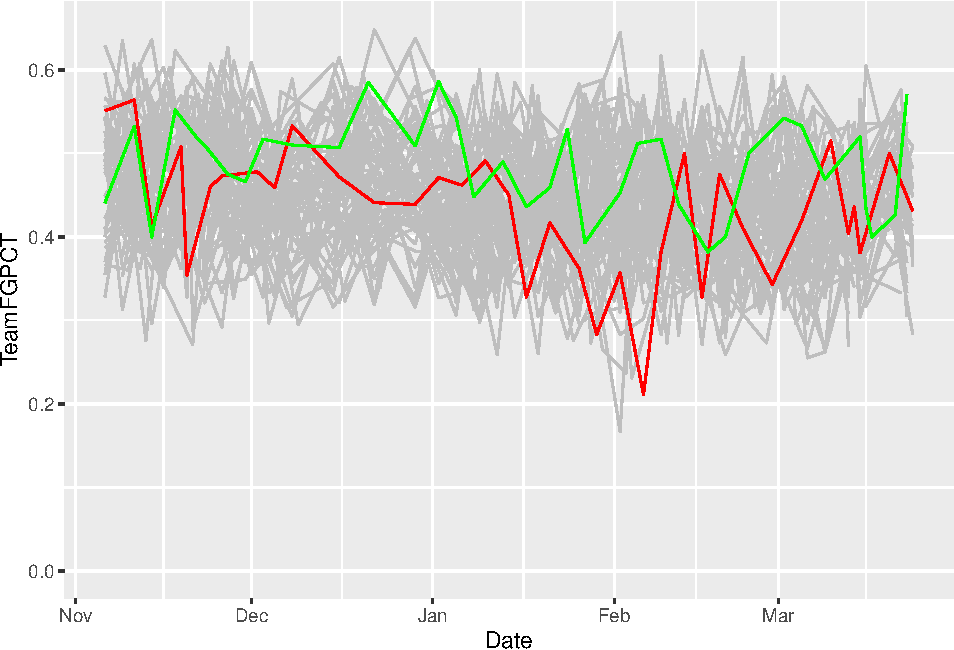
\includegraphics{SportsData_files/figure-latex/unnamed-chunk-139-1.pdf}

What do we see here? How has Nebraska and Michigan State's season evolved against all the rest of the teams in college basketball?

But how does that compare to the average? We can add that pretty easily by creating a new dataframe with it and add another geom\_line.

\begin{Shaded}
\begin{Highlighting}[]
\NormalTok{average <-}\StringTok{ }\NormalTok{logs }\OperatorTok\StringTok{ }\KeywordTok{group_by}\NormalTok{(Date) }\OperatorTok\StringTok{ }\KeywordTok{summarise}\NormalTok{(}\DataTypeTok{mean_shooting=}\KeywordTok{mean}\NormalTok{(TeamFGPCT))}
\end{Highlighting}
\end{Shaded}

\begin{Shaded}
\begin{Highlighting}[]
\KeywordTok{ggplot}\NormalTok{() }\OperatorTok{+}\StringTok{ }\KeywordTok{geom_line}\NormalTok{(}\DataTypeTok{data=}\NormalTok{p5conf, }\KeywordTok{aes}\NormalTok{(}\DataTypeTok{x=}\NormalTok{Date, }\DataTypeTok{y=}\NormalTok{TeamFGPCT, }\DataTypeTok{group=}\NormalTok{Team), }\DataTypeTok{color=}\StringTok{"grey"}\NormalTok{) }\OperatorTok{+}\StringTok{ }\KeywordTok{geom_line}\NormalTok{(}\DataTypeTok{data=}\NormalTok{nu, }\KeywordTok{aes}\NormalTok{(}\DataTypeTok{x=}\NormalTok{Date, }\DataTypeTok{y=}\NormalTok{TeamFGPCT), }\DataTypeTok{color=}\StringTok{"red"}\NormalTok{) }\OperatorTok{+}\StringTok{ }\KeywordTok{geom_line}\NormalTok{(}\DataTypeTok{data=}\NormalTok{msu, }\KeywordTok{aes}\NormalTok{(}\DataTypeTok{x=}\NormalTok{Date, }\DataTypeTok{y=}\NormalTok{TeamFGPCT), }\DataTypeTok{color=}\StringTok{"green"}\NormalTok{) }\OperatorTok{+}\StringTok{ }\KeywordTok{geom_line}\NormalTok{(}\DataTypeTok{data=}\NormalTok{average, }\KeywordTok{aes}\NormalTok{(}\DataTypeTok{x=}\NormalTok{Date, }\DataTypeTok{y=}\NormalTok{mean_shooting), }\DataTypeTok{color=}\StringTok{"black"}\NormalTok{) }\OperatorTok{+}\StringTok{ }\KeywordTok{scale_y_continuous}\NormalTok{(}\DataTypeTok{limits =} \KeywordTok{c}\NormalTok{(}\DecValTok{0}\NormalTok{, }\FloatTok{.65}\NormalTok{))}
\end{Highlighting}
\end{Shaded}

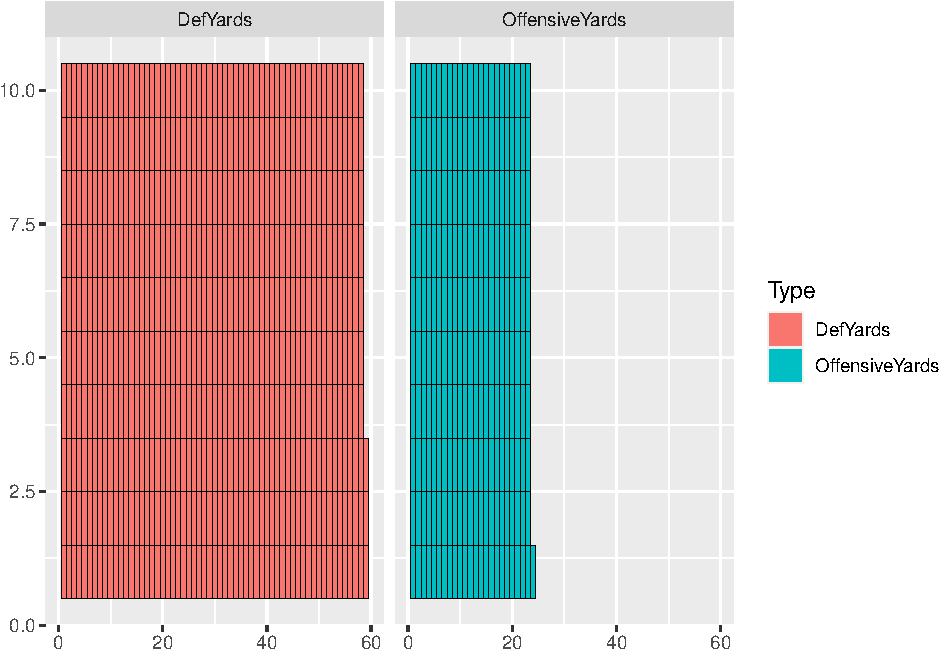
\includegraphics{SportsData_files/figure-latex/unnamed-chunk-141-1.pdf}

\hypertarget{step-charts}{%
\chapter{Step charts}\label{step-charts}}

Step charts are \textbf{a method of showing progress} toward something. They combine showing change over time -- \textbf{cumulative change over time} -- with magnitude. They're good at inviting comparison.

There's great examples out there. First is the Washignton Post looking at \href{https://www.washingtonpost.com/graphics/sports/lebron-james-michael-jordan-nba-scoring-list/?utm_term=.481074150849}{Lebron passing Jordan's career point total}. Another is John Burn-Murdoch's work at the Financial Times (which is paywalled) about soccer stars. \href{http://johnburnmurdoch.github.io/projects/goal-lines/CL/}{Here's an example of his work outside the paywall}.

To replicate this, we need cumulative data -- data that is the running total of data at a given point. So think of it this way -- Nebraska scores 50 points in a basketball game and then 50 more the next, their cumulative total at two games is 100 points.

Step charts can be used for all kinds of things -- showing how a player's career has evolved over time, how a team fares over a season, or franchise history. Let's walk through an example.

\begin{Shaded}
\begin{Highlighting}[]
\KeywordTok{library}\NormalTok{(tidyverse)}
\end{Highlighting}
\end{Shaded}

And we'll use \href{https://unl.box.com/s/a8m91bro10t89watsyo13yjegb1fy009}{our basketball log data}.

\begin{Shaded}
\begin{Highlighting}[]
\NormalTok{logs <-}\StringTok{ }\KeywordTok{read_csv}\NormalTok{(}\StringTok{"data/logs19.csv"}\NormalTok{)}
\end{Highlighting}
\end{Shaded}

\begin{verbatim}
## Warning: Missing column names filled in: 'X1' [1]
\end{verbatim}

\begin{verbatim}
## Parsed with column specification:
## cols(
##   .default = col_double(),
##   Date = col_date(format = ""),
##   HomeAway = col_character(),
##   Opponent = col_character(),
##   W_L = col_character(),
##   Blank = col_logical(),
##   Team = col_character(),
##   Conference = col_character(),
##   season = col_character()
## )
\end{verbatim}

\begin{verbatim}
## See spec(...) for full column specifications.
\end{verbatim}

Here we're going to look at the scoring differential of teams. If you score more than your opponent, you win. So it stands to reason that if you score a lot more than your opponent over the course of a season, you should be very good, right? Let's see.

The first thing we're going to do is calculate that differential. Then, we'll group it by the team. After that, we're going to summarize using a new function called \texttt{cumsum} or cumulative sum -- the sum for each game as we go forward. So game 1's cumsum is the differential of that game. Game 2's cumsum is Game 1 + Game 2. Game 3 is Game 1 + 2 + 3 and so on.

\begin{Shaded}
\begin{Highlighting}[]
\NormalTok{difflogs <-}\StringTok{ }\NormalTok{logs }\OperatorTok\StringTok{ }
\StringTok{  }\KeywordTok{mutate}\NormalTok{(}\DataTypeTok{Differential =}\NormalTok{ TeamScore }\OperatorTok{-}\StringTok{ }\NormalTok{OpponentScore) }\OperatorTok\StringTok{ }
\StringTok{  }\KeywordTok{group_by}\NormalTok{(Team) }\OperatorTok\StringTok{ }
\StringTok{  }\KeywordTok{mutate}\NormalTok{(}\DataTypeTok{CumDiff =} \KeywordTok{cumsum}\NormalTok{(Differential))}
\end{Highlighting}
\end{Shaded}

Now that we have the cumulative sum for each, let's filter it down to just Big Ten teams.

\begin{Shaded}
\begin{Highlighting}[]
\NormalTok{bigdiff <-}\StringTok{ }\NormalTok{difflogs }\OperatorTok\StringTok{ }\KeywordTok{filter}\NormalTok{(Conference }\OperatorTok{==}\StringTok{ "Big Ten"}\NormalTok{)}
\end{Highlighting}
\end{Shaded}

The step chart is it's own geom, so we can employ it just like we have the others. It works almost exactly the same as a line chart, but it uses the cumulative sum instead of a regular value and, as the name implies, creates a step like shape to the line instead of a curve.

\begin{Shaded}
\begin{Highlighting}[]
\KeywordTok{ggplot}\NormalTok{() }\OperatorTok{+}\StringTok{ }\KeywordTok{geom_step}\NormalTok{(}\DataTypeTok{data=}\NormalTok{bigdiff, }\KeywordTok{aes}\NormalTok{(}\DataTypeTok{x=}\NormalTok{Date, }\DataTypeTok{y=}\NormalTok{CumDiff, }\DataTypeTok{group=}\NormalTok{Team))}
\end{Highlighting}
\end{Shaded}

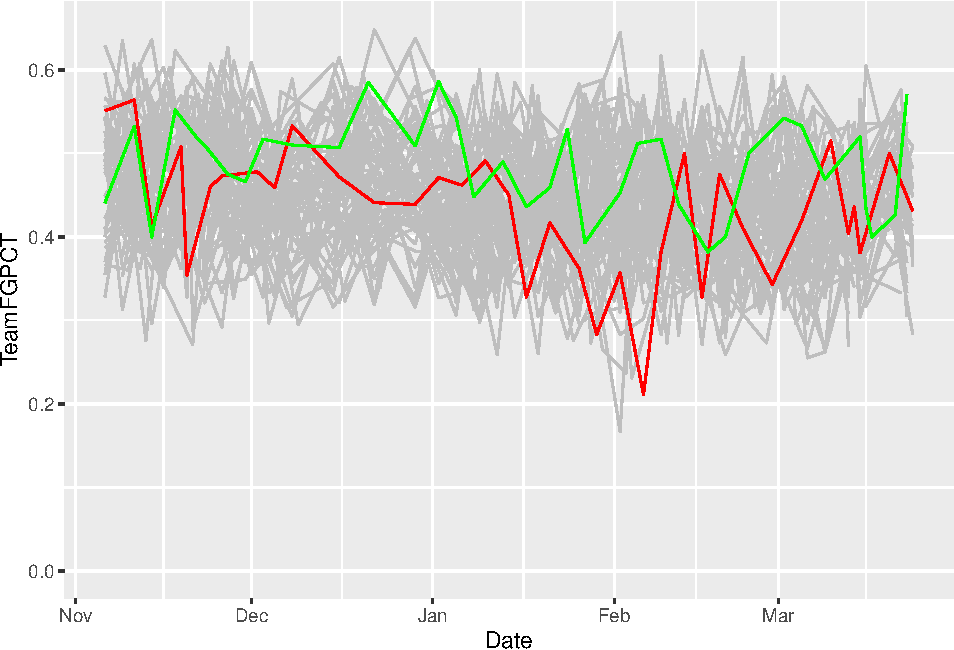
\includegraphics{SportsData_files/figure-latex/unnamed-chunk-146-1.pdf}

Let's try a different element of the aesthetic: color, but this time inside the aesthetic. Last time, we did the color outside. When you put it inside, you pass it a column name and ggplot will color each line based on what thing that is, and it will create a legend that labels each line that thing.

\begin{Shaded}
\begin{Highlighting}[]
\KeywordTok{ggplot}\NormalTok{() }\OperatorTok{+}\StringTok{ }\KeywordTok{geom_step}\NormalTok{(}\DataTypeTok{data=}\NormalTok{bigdiff, }\KeywordTok{aes}\NormalTok{(}\DataTypeTok{x=}\NormalTok{Date, }\DataTypeTok{y=}\NormalTok{CumDiff, }\DataTypeTok{group=}\NormalTok{Team, }\DataTypeTok{color=}\NormalTok{Team))}
\end{Highlighting}
\end{Shaded}

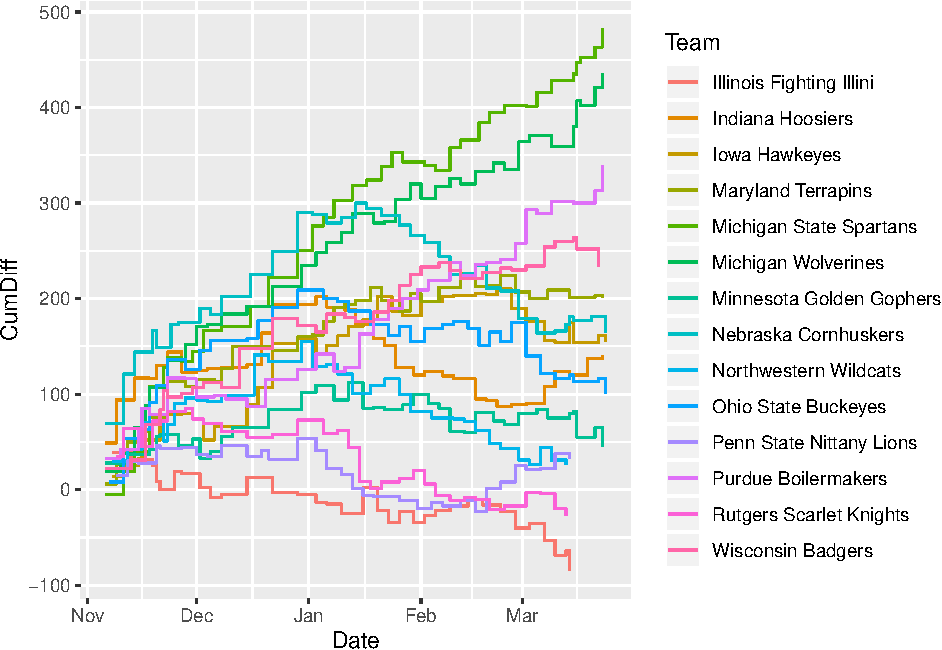
\includegraphics{SportsData_files/figure-latex/unnamed-chunk-147-1.pdf}

From this, we can see two teams in the Big Ten had negative point differentials last season -- Illinois and Rutgers.

Let's look at those top teams plus Nebraska.

\begin{Shaded}
\begin{Highlighting}[]
\NormalTok{nu <-}\StringTok{ }\NormalTok{bigdiff }\OperatorTok\StringTok{ }\KeywordTok{filter}\NormalTok{(Team }\OperatorTok{==}\StringTok{ "Nebraska Cornhuskers"}\NormalTok{)}
\NormalTok{mi <-}\StringTok{ }\NormalTok{bigdiff }\OperatorTok\StringTok{ }\KeywordTok{filter}\NormalTok{(Team }\OperatorTok{==}\StringTok{ "Michigan Wolverines"}\NormalTok{)}
\NormalTok{ms <-}\StringTok{ }\NormalTok{bigdiff }\OperatorTok\StringTok{ }\KeywordTok{filter}\NormalTok{(Team }\OperatorTok{==}\StringTok{ "Michigan State Spartans"}\NormalTok{)}
\end{Highlighting}
\end{Shaded}

Let's introduce a couple of new things here. First, note when I take the color OUT of the aesthetic, the legend disappears.

The second thing I'm going to add is the annotation layer. In this case, I am adding a text annotation layer, and I can specify where by adding in a x and a y value where I want to put it. This takes some finesse. After that, I'm going to add labels and a theme.

\begin{Shaded}
\begin{Highlighting}[]
\KeywordTok{ggplot}\NormalTok{() }\OperatorTok{+}\StringTok{ }
\StringTok{  }\KeywordTok{geom_step}\NormalTok{(}\DataTypeTok{data=}\NormalTok{bigdiff, }\KeywordTok{aes}\NormalTok{(}\DataTypeTok{x=}\NormalTok{Date, }\DataTypeTok{y=}\NormalTok{CumDiff, }\DataTypeTok{group=}\NormalTok{Team), }\DataTypeTok{color=}\StringTok{"light grey"}\NormalTok{) }\OperatorTok{+}
\StringTok{  }\KeywordTok{geom_step}\NormalTok{(}\DataTypeTok{data=}\NormalTok{nu, }\KeywordTok{aes}\NormalTok{(}\DataTypeTok{x=}\NormalTok{Date, }\DataTypeTok{y=}\NormalTok{CumDiff, }\DataTypeTok{group=}\NormalTok{Team), }\DataTypeTok{color=}\StringTok{"red"}\NormalTok{) }\OperatorTok{+}\StringTok{ }
\StringTok{  }\KeywordTok{geom_step}\NormalTok{(}\DataTypeTok{data=}\NormalTok{mi, }\KeywordTok{aes}\NormalTok{(}\DataTypeTok{x=}\NormalTok{Date, }\DataTypeTok{y=}\NormalTok{CumDiff, }\DataTypeTok{group=}\NormalTok{Team), }\DataTypeTok{color=}\StringTok{"blue"}\NormalTok{) }\OperatorTok{+}\StringTok{ }
\StringTok{  }\KeywordTok{geom_step}\NormalTok{(}\DataTypeTok{data=}\NormalTok{ms, }\KeywordTok{aes}\NormalTok{(}\DataTypeTok{x=}\NormalTok{Date, }\DataTypeTok{y=}\NormalTok{CumDiff, }\DataTypeTok{group=}\NormalTok{Team), }\DataTypeTok{color=}\StringTok{"green"}\NormalTok{) }\OperatorTok{+}
\StringTok{  }\KeywordTok{annotate}\NormalTok{(}\StringTok{"text"}\NormalTok{, }\DataTypeTok{x=}\NormalTok{(}\KeywordTok{as.Date}\NormalTok{(}\StringTok{"2018-12-10"}\NormalTok{)), }\DataTypeTok{y=}\DecValTok{220}\NormalTok{, }\DataTypeTok{label=}\StringTok{"Nebraska"}\NormalTok{) }\OperatorTok{+}
\StringTok{  }\KeywordTok{labs}\NormalTok{(}\DataTypeTok{x=}\StringTok{"Date"}\NormalTok{, }\DataTypeTok{y=}\StringTok{"Cumulative Point Differential"}\NormalTok{, }\DataTypeTok{title=}\StringTok{"Nebraska was among the league's most dominant"}\NormalTok{, }\DataTypeTok{subtitle=}\StringTok{"Before the misseason skid, Nebraska was at the top of the Big Ten in point differential"}\NormalTok{, }\DataTypeTok{caption=}\StringTok{"Source: Sports-Reference.com | By Matt Waite"}\NormalTok{) }\OperatorTok{+}
\StringTok{  }\KeywordTok{theme_minimal}\NormalTok{()}
\end{Highlighting}
\end{Shaded}

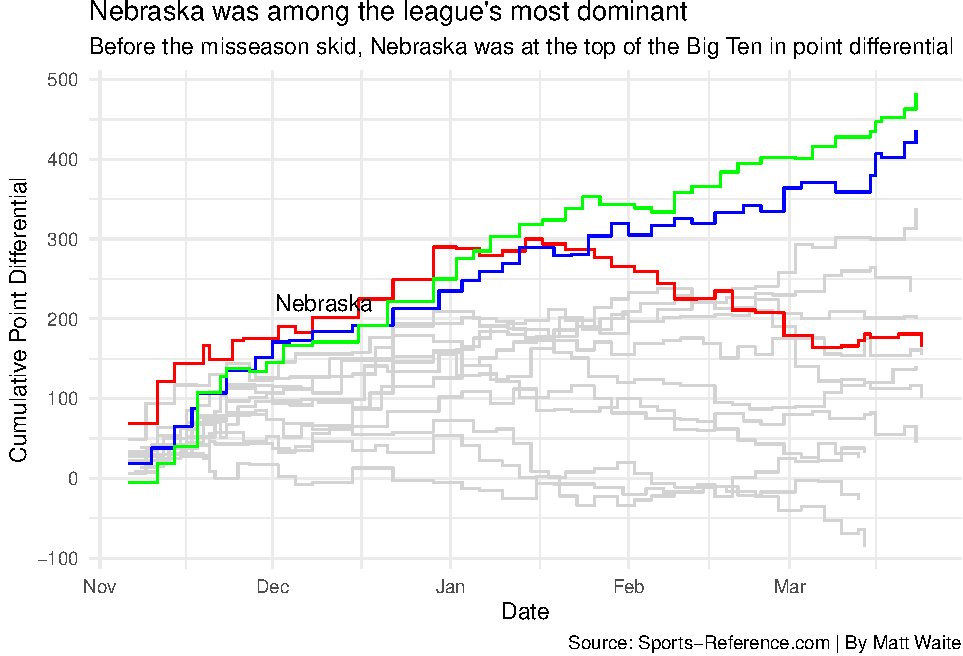
\includegraphics{SportsData_files/figure-latex/unnamed-chunk-149-1.pdf}

\hypertarget{ridge-charts}{%
\chapter{Ridge charts}\label{ridge-charts}}

Ridgeplots are useful for when you want to show how different groupings compare with a large number of datapoints. So let's look at how we do this, and in the process, we learn about ggplot extensions. The extensions add functionality to ggplot, which doesn't out of the box have ridgeplots (sometimes called joyplots).

In the console, run this: \texttt{install.packages("ggridges")}

Now we can add those libraries.

\begin{Shaded}
\begin{Highlighting}[]
\KeywordTok{library}\NormalTok{(tidyverse)}
\KeywordTok{library}\NormalTok{(ggridges)}
\end{Highlighting}
\end{Shaded}

So for this, let's look at every basketball game played since the 2014-15 season. That's more than 28,000 basketball games. \href{https://unl.box.com/s/u9407jj007fxtnu1vbkybdawaqg6j3fw}{Download that data here}.

\begin{Shaded}
\begin{Highlighting}[]
\NormalTok{logs <-}\StringTok{ }\KeywordTok{read_csv}\NormalTok{(}\StringTok{"data/logs1519.csv"}\NormalTok{)}
\end{Highlighting}
\end{Shaded}

\begin{verbatim}
## Warning: Missing column names filled in: 'X1' [1]
\end{verbatim}

\begin{verbatim}
## Parsed with column specification:
## cols(
##   .default = col_double(),
##   Date = col_date(format = ""),
##   HomeAway = col_character(),
##   Opponent = col_character(),
##   W_L = col_character(),
##   Blank = col_logical(),
##   Team = col_character(),
##   Conference = col_character(),
##   season = col_character()
## )
\end{verbatim}

\begin{verbatim}
## See spec(...) for full column specifications.
\end{verbatim}

So I want to group teams by wins. Wins are the only thing that matter -- ask Tim Miles. So our data has a column called W\_L that lists if the team won or lost. The problem is it doesn't just say W or L. If the game went to overtime, it lists that. That complicates counting wins. And, with ridgeplots, I want to be be able to separate EVERY GAME by how many wins the team had over a SEASON. So I've got some work to do.

First, here's a trick to find a string of text and make that. It's called \texttt{grepl} and the basic syntax is grepl for this string in this field and then do what I tell you. In this case, we're going to create a new field called winloss look for W or L (and ignore any OT notation) and give wins a 1 and losses a 0.

\begin{Shaded}
\begin{Highlighting}[]
\NormalTok{winlosslogs <-}\StringTok{ }\NormalTok{logs }\OperatorTok\StringTok{ }\KeywordTok{mutate}\NormalTok{(}\DataTypeTok{winloss =} \KeywordTok{case_when}\NormalTok{(}
  \KeywordTok{grepl}\NormalTok{(}\StringTok{"W"}\NormalTok{, W_L) }\OperatorTok{~}\StringTok{ }\DecValTok{1}\NormalTok{, }
  \KeywordTok{grepl}\NormalTok{(}\StringTok{"L"}\NormalTok{, W_L) }\OperatorTok{~}\StringTok{ }\DecValTok{0}\NormalTok{)}
\NormalTok{)}
\end{Highlighting}
\end{Shaded}

Now I'm going to add up all the winlosses for each team, which should give me the number of wins for each team.

\begin{Shaded}
\begin{Highlighting}[]
\NormalTok{winlosslogs }\OperatorTok\StringTok{ }\KeywordTok{group_by}\NormalTok{(Team, Conference, season) }\OperatorTok\StringTok{ }\KeywordTok{summarise}\NormalTok{(}\DataTypeTok{TeamWins =} \KeywordTok{sum}\NormalTok{(winloss)) ->}\StringTok{ }\NormalTok{teamseasonwins}
\end{Highlighting}
\end{Shaded}

Now that I have season win totals, I can join that data back to my log data so each game has the total number of wins in each season.

\begin{Shaded}
\begin{Highlighting}[]
\NormalTok{winlosslogs }\OperatorTok\StringTok{ }\KeywordTok{left_join}\NormalTok{(teamseasonwins, }\DataTypeTok{by=}\KeywordTok{c}\NormalTok{(}\StringTok{"Team"}\NormalTok{, }\StringTok{"Conference"}\NormalTok{, }\StringTok{"season"}\NormalTok{)) ->}\StringTok{ }\NormalTok{wintotallogs}
\end{Highlighting}
\end{Shaded}

Now I can use that same \texttt{case\_when} logic to create some groupings. So I want to group teams together by how many wins they had over the season. For no good reason, I started with more than 25 wins, then did groups of 5 down to 10 wins. If you had fewer than 10 wins, God help your program.

The way to create a new field based on groupings like that is to use \texttt{case\_when}, which says, basically, when This Thing Is True, Do This. So in our case, we're going to pass a couple of logical statements that when they are both true, our data gets labeled how we want to label it. So we \texttt{mutate} a field called grouping and then use \texttt{case\_when}.

\begin{Shaded}
\begin{Highlighting}[]
\NormalTok{wintotallogs }\OperatorTok\StringTok{ }\KeywordTok{mutate}\NormalTok{(}\DataTypeTok{grouping =} \KeywordTok{case_when}\NormalTok{(}
\NormalTok{  TeamWins }\OperatorTok{>}\StringTok{ }\DecValTok{25} \OperatorTok{~}\StringTok{ "More than 25 wins"}\NormalTok{,}
\NormalTok{  TeamWins }\OperatorTok{>=}\StringTok{ }\DecValTok{20} \OperatorTok{&}\StringTok{ }\NormalTok{TeamWins }\OperatorTok{<=}\DecValTok{25} \OperatorTok{~}\StringTok{ "20-25 wins"}\NormalTok{,}
\NormalTok{  TeamWins }\OperatorTok{>=}\StringTok{ }\DecValTok{15} \OperatorTok{&}\StringTok{ }\NormalTok{TeamWins }\OperatorTok{<=}\DecValTok{19} \OperatorTok{~}\StringTok{ "15-19 wins"}\NormalTok{,}
\NormalTok{  TeamWins }\OperatorTok{>=}\StringTok{ }\DecValTok{10} \OperatorTok{&}\StringTok{ }\NormalTok{TeamWins }\OperatorTok{<=}\DecValTok{14} \OperatorTok{~}\StringTok{ "10-14 wins"}\NormalTok{,}
\NormalTok{  TeamWins }\OperatorTok{<}\StringTok{ }\DecValTok{10} \OperatorTok{~}\StringTok{ "Less than 10 wins"}\NormalTok{)}
\NormalTok{) ->}\StringTok{ }\NormalTok{wintotalgroupinglogs}
\end{Highlighting}
\end{Shaded}

So my \texttt{wintotalgroupinglogs} table has each game, with a field that gives the total number of wins each team had that season and labeling each game with one of five groupings. I could use \texttt{dplyr} to do group\_by on those five groups and find some things out about them, but ridgeplots do that visually.

Let's look at the differences in rebounds by those five groups. Do teams that win more than 25 games rebound better than teams that win fewer games?

The answer might surprise you.

\begin{Shaded}
\begin{Highlighting}[]
\KeywordTok{ggplot}\NormalTok{(wintotalgroupinglogs, }\KeywordTok{aes}\NormalTok{(}\DataTypeTok{x =}\NormalTok{ TeamTotalRebounds, }\DataTypeTok{y =}\NormalTok{ grouping, }\DataTypeTok{fill =}\NormalTok{ grouping)) }\OperatorTok{+}
\StringTok{  }\KeywordTok{geom_density_ridges}\NormalTok{() }\OperatorTok{+}
\StringTok{  }\KeywordTok{theme_ridges}\NormalTok{() }\OperatorTok{+}\StringTok{ }
\StringTok{  }\KeywordTok{theme}\NormalTok{(}\DataTypeTok{legend.position =} \StringTok{"none"}\NormalTok{)}
\end{Highlighting}
\end{Shaded}

\begin{verbatim}
## Picking joint bandwidth of 0.88
\end{verbatim}

\begin{verbatim}
## Warning: Removed 2 rows containing non-finite values (stat_density_ridges).
\end{verbatim}

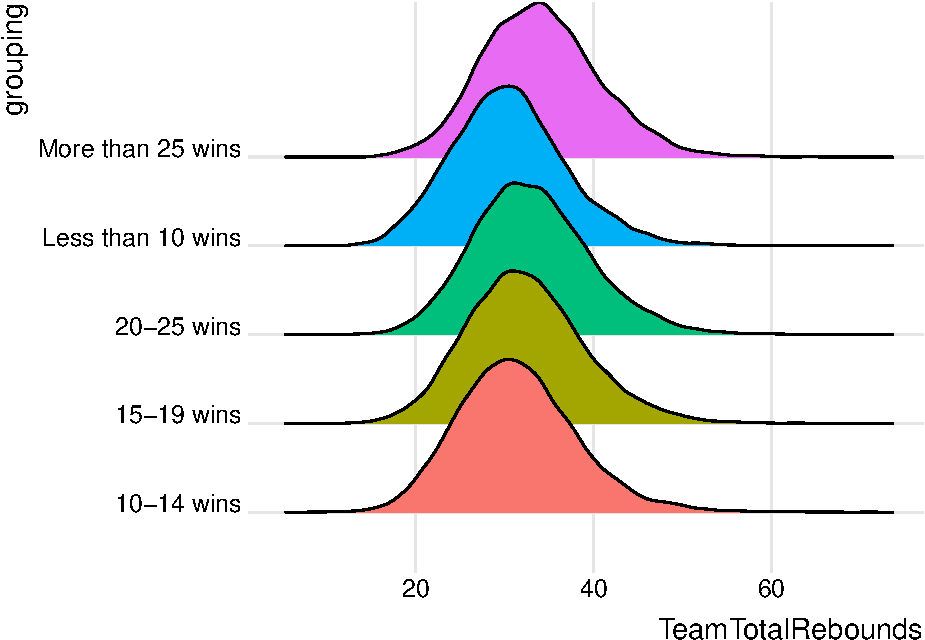
\includegraphics{SportsData_files/figure-latex/unnamed-chunk-156-1.pdf}

Answer? Not really. Game to game, maybe. Over five seasons? The differences are indistinguishable.

How about assists?

\begin{Shaded}
\begin{Highlighting}[]
\KeywordTok{ggplot}\NormalTok{(wintotalgroupinglogs, }\KeywordTok{aes}\NormalTok{(}\DataTypeTok{x =}\NormalTok{ TeamAssists, }\DataTypeTok{y =}\NormalTok{ grouping, }\DataTypeTok{fill =}\NormalTok{ grouping)) }\OperatorTok{+}
\StringTok{  }\KeywordTok{geom_density_ridges}\NormalTok{() }\OperatorTok{+}
\StringTok{  }\KeywordTok{theme_ridges}\NormalTok{() }\OperatorTok{+}\StringTok{ }
\StringTok{  }\KeywordTok{theme}\NormalTok{(}\DataTypeTok{legend.position =} \StringTok{"none"}\NormalTok{)}
\end{Highlighting}
\end{Shaded}

\begin{verbatim}
## Picking joint bandwidth of 0.601
\end{verbatim}

\begin{verbatim}
## Warning: Removed 2 rows containing non-finite values (stat_density_ridges).
\end{verbatim}

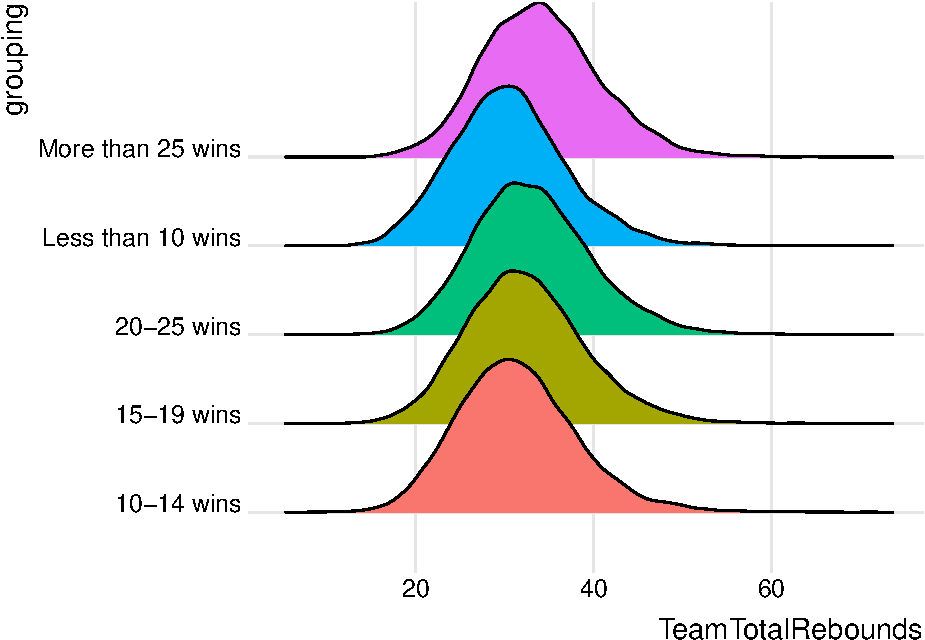
\includegraphics{SportsData_files/figure-latex/unnamed-chunk-157-1.pdf}

There's a little better, especially between top and bottom.

\begin{Shaded}
\begin{Highlighting}[]
\KeywordTok{ggplot}\NormalTok{(wintotalgroupinglogs, }\KeywordTok{aes}\NormalTok{(}\DataTypeTok{x =}\NormalTok{ Team3PPCT, }\DataTypeTok{y =}\NormalTok{ grouping, }\DataTypeTok{fill =}\NormalTok{ grouping)) }\OperatorTok{+}
\StringTok{  }\KeywordTok{geom_density_ridges}\NormalTok{() }\OperatorTok{+}
\StringTok{  }\KeywordTok{theme_ridges}\NormalTok{() }\OperatorTok{+}\StringTok{ }
\StringTok{  }\KeywordTok{theme}\NormalTok{(}\DataTypeTok{legend.position =} \StringTok{"none"}\NormalTok{)}
\end{Highlighting}
\end{Shaded}

\begin{verbatim}
## Picking joint bandwidth of 0.0156
\end{verbatim}

\begin{verbatim}
## Warning: Removed 2 rows containing non-finite values (stat_density_ridges).
\end{verbatim}

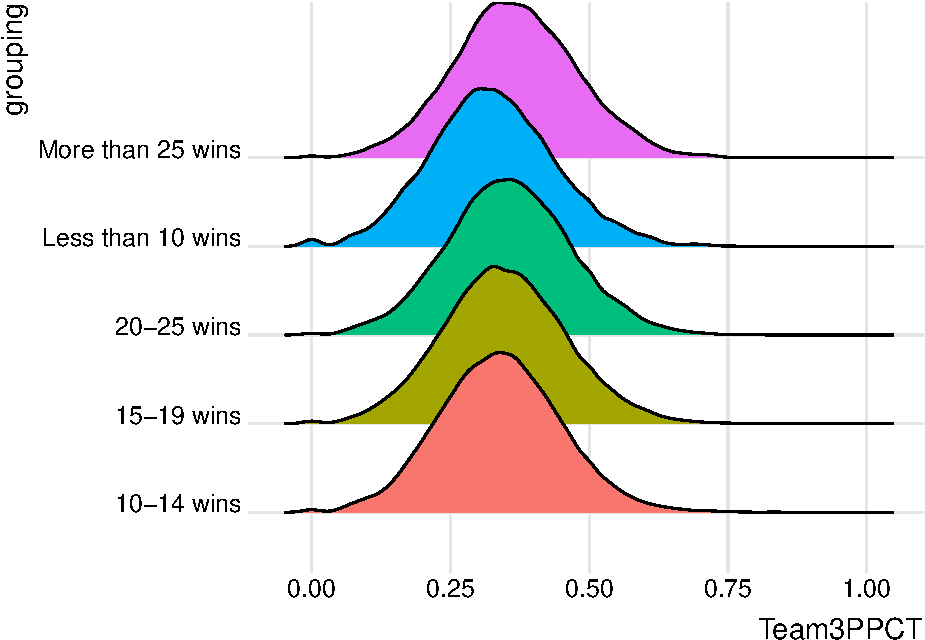
\includegraphics{SportsData_files/figure-latex/unnamed-chunk-158-1.pdf}

If you've been paying attention this semester, you know what's coming next.

\begin{Shaded}
\begin{Highlighting}[]
\KeywordTok{ggplot}\NormalTok{(wintotalgroupinglogs, }\KeywordTok{aes}\NormalTok{(}\DataTypeTok{x =}\NormalTok{ TeamFGPCT, }\DataTypeTok{y =}\NormalTok{ grouping, }\DataTypeTok{fill =}\NormalTok{ grouping)) }\OperatorTok{+}
\StringTok{  }\KeywordTok{geom_density_ridges}\NormalTok{() }\OperatorTok{+}
\StringTok{  }\KeywordTok{theme_ridges}\NormalTok{() }\OperatorTok{+}\StringTok{ }
\StringTok{  }\KeywordTok{theme}\NormalTok{(}\DataTypeTok{legend.position =} \StringTok{"none"}\NormalTok{)}
\end{Highlighting}
\end{Shaded}

\begin{verbatim}
## Picking joint bandwidth of 0.0102
\end{verbatim}

\begin{verbatim}
## Warning: Removed 2 rows containing non-finite values (stat_density_ridges).
\end{verbatim}

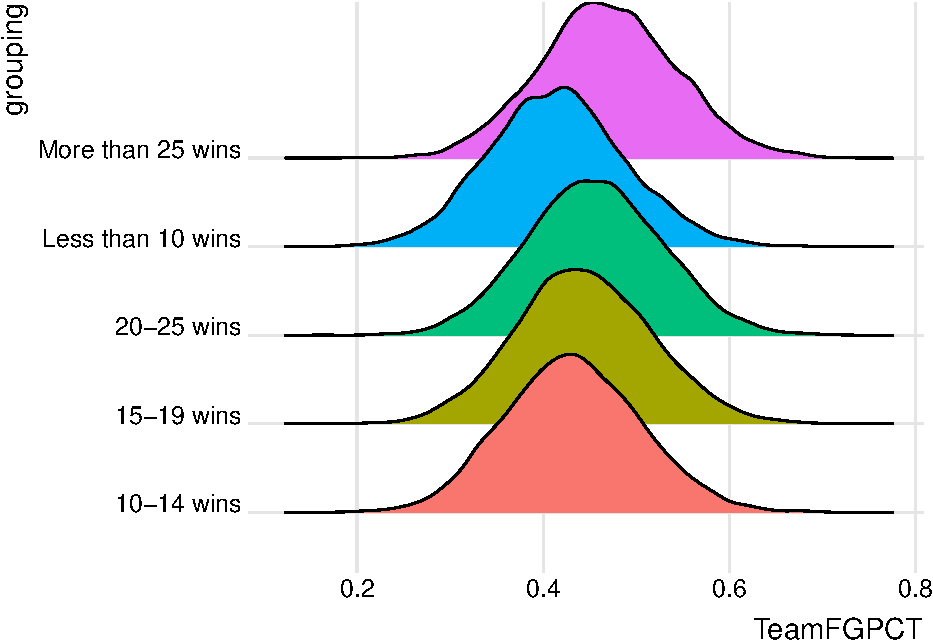
\includegraphics{SportsData_files/figure-latex/unnamed-chunk-159-1.pdf}

\hypertarget{lollipop-charts}{%
\chapter{Lollipop charts}\label{lollipop-charts}}

Second to my love of waffle charts because I'm always hungry, lollipop charts are an excellently named way of showing the difference between two things on a number line -- a start and a finish, for instance. Or the difference between two related things. Say, turnovers and assists. They aren't a geom, specifically, but you can assemble them out of points and segments, which are geoms.

\begin{Shaded}
\begin{Highlighting}[]
\KeywordTok{library}\NormalTok{(tidyverse)}
\end{Highlighting}
\end{Shaded}

\begin{Shaded}
\begin{Highlighting}[]
\NormalTok{logs <-}\StringTok{ }\KeywordTok{read_csv}\NormalTok{(}\StringTok{"data/logs19.csv"}\NormalTok{)}
\end{Highlighting}
\end{Shaded}

\begin{verbatim}
## Warning: Missing column names filled in: 'X1' [1]
\end{verbatim}

\begin{verbatim}
## Parsed with column specification:
## cols(
##   .default = col_double(),
##   Date = col_date(format = ""),
##   HomeAway = col_character(),
##   Opponent = col_character(),
##   W_L = col_character(),
##   Blank = col_logical(),
##   Team = col_character(),
##   Conference = col_character(),
##   season = col_character()
## )
\end{verbatim}

\begin{verbatim}
## See spec(...) for full column specifications.
\end{verbatim}

For the first example, let's look at the difference between a team's shooting performance and the conference's shooting performance as a whole. To get this, we're going to add up all the shots made by the conference, all the attempts taken by the conference, and then mutate a percentage based on that.

\begin{Shaded}
\begin{Highlighting}[]
\NormalTok{conferenceshooting <-}\StringTok{ }\NormalTok{logs }\OperatorTok
\StringTok{  }\KeywordTok{group_by}\NormalTok{(Conference) }\OperatorTok\StringTok{ }
\StringTok{  }\KeywordTok{summarise}\NormalTok{(}\DataTypeTok{totalshots =} \KeywordTok{sum}\NormalTok{(TeamFG), }\DataTypeTok{totalattempts =} \KeywordTok{sum}\NormalTok{(TeamFGA)) }\OperatorTok
\StringTok{  }\KeywordTok{mutate}\NormalTok{(}\DataTypeTok{conferenceshootingpct =}\NormalTok{ totalshots}\OperatorTok{/}\NormalTok{totalattempts)}
\end{Highlighting}
\end{Shaded}

Now I'm going to do the same with teams.

\begin{Shaded}
\begin{Highlighting}[]
\NormalTok{teamshooting <-}\StringTok{ }\NormalTok{logs }\OperatorTok
\StringTok{  }\KeywordTok{group_by}\NormalTok{(Team, Conference) }\OperatorTok\StringTok{ }
\StringTok{  }\KeywordTok{summarise}\NormalTok{(}\DataTypeTok{totalshots =} \KeywordTok{sum}\NormalTok{(TeamFG), }\DataTypeTok{totalattempts =} \KeywordTok{sum}\NormalTok{(TeamFGA)) }\OperatorTok
\StringTok{  }\KeywordTok{mutate}\NormalTok{(}\DataTypeTok{teamshootingpct =}\NormalTok{ totalshots}\OperatorTok{/}\NormalTok{totalattempts)}
\end{Highlighting}
\end{Shaded}

The last thing I need to do is join them together. So each team will have the conference shooting percentage as well as their own.

\begin{Shaded}
\begin{Highlighting}[]
\NormalTok{shooting <-}\StringTok{ }\NormalTok{teamshooting }\OperatorTok\StringTok{ }\KeywordTok{left_join}\NormalTok{(conferenceshooting, }\DataTypeTok{by=}\StringTok{"Conference"}\NormalTok{)}
\end{Highlighting}
\end{Shaded}

I have every team in college basketball, but that's insane.

\begin{Shaded}
\begin{Highlighting}[]
\NormalTok{big10 <-}\StringTok{ }\NormalTok{shooting }\OperatorTok\StringTok{ }\KeywordTok{filter}\NormalTok{(Conference }\OperatorTok{==}\StringTok{ "Big Ten"}\NormalTok{)}
\end{Highlighting}
\end{Shaded}

So this takes a little doing, but the logic is pretty clear in the end.

A lollipop chart is made up of two things -- a line between two points, and two points. So we need a geom\_segment and two geom\_points. And because they get layered starting at the bottom, our segment is first. A geom segment is made up of two things -- an x and a y value, and an x and y end. In this case, our x and xend are the same -- the Team -- and our y and yend are our two stats. For our points, both x values are the Team and the y is the different stats. What that does is put each point on the same line.

\begin{Shaded}
\begin{Highlighting}[]
\KeywordTok{ggplot}\NormalTok{(big10) }\OperatorTok{+}
\StringTok{  }\KeywordTok{geom_segment}\NormalTok{(}\KeywordTok{aes}\NormalTok{(}\DataTypeTok{x=}\NormalTok{Team, }\DataTypeTok{xend=}\NormalTok{Team, }\DataTypeTok{y=}\NormalTok{teamshootingpct, }\DataTypeTok{yend=}\NormalTok{conferenceshootingpct), }\DataTypeTok{color=}\StringTok{"grey"}\NormalTok{) }\OperatorTok{+}\StringTok{ }
\StringTok{  }\KeywordTok{geom_point}\NormalTok{(}\KeywordTok{aes}\NormalTok{(}\DataTypeTok{x=}\NormalTok{Team, }\DataTypeTok{y=}\NormalTok{teamshootingpct), }\DataTypeTok{color=}\StringTok{"red"}\NormalTok{) }\OperatorTok{+}\StringTok{ }
\StringTok{  }\KeywordTok{geom_point}\NormalTok{(}\KeywordTok{aes}\NormalTok{(}\DataTypeTok{x=}\NormalTok{Team, }\DataTypeTok{y=}\NormalTok{conferenceshootingpct), }\DataTypeTok{color=}\StringTok{"blue"}\NormalTok{) }\OperatorTok{+}
\StringTok{  }\KeywordTok{coord_flip}\NormalTok{()}
\end{Highlighting}
\end{Shaded}

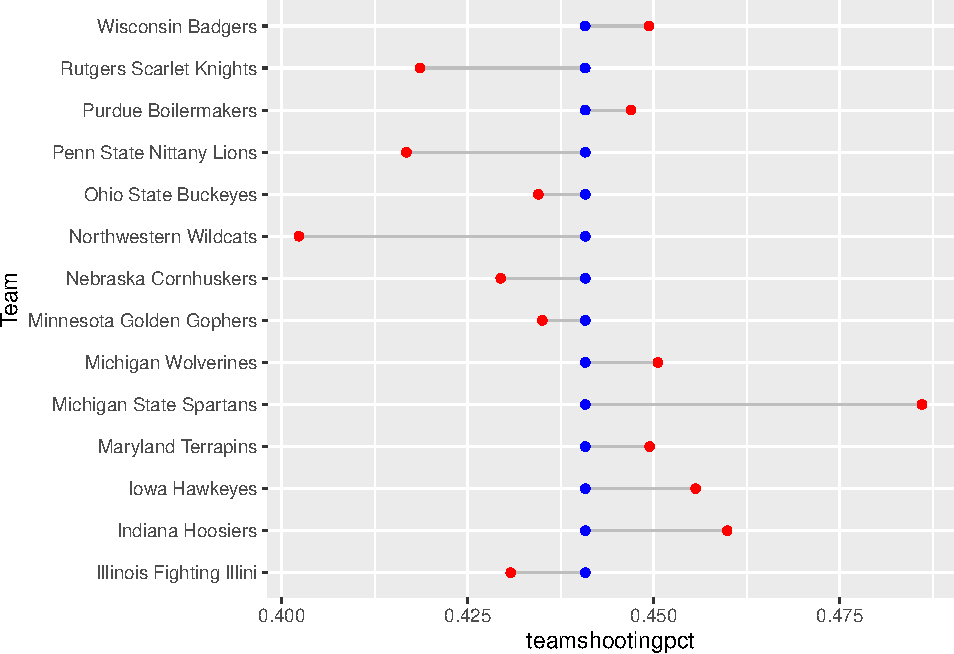
\includegraphics{SportsData_files/figure-latex/unnamed-chunk-166-1.pdf}

We can do better by changing the order of the teams by their shooting performance and giving it some theme love.

\begin{Shaded}
\begin{Highlighting}[]
\KeywordTok{ggplot}\NormalTok{(big10) }\OperatorTok{+}
\StringTok{  }\KeywordTok{geom_segment}\NormalTok{(}\KeywordTok{aes}\NormalTok{(}\DataTypeTok{x=}\KeywordTok{reorder}\NormalTok{(Team, teamshootingpct), }\DataTypeTok{xend=}\NormalTok{Team, }\DataTypeTok{y=}\NormalTok{teamshootingpct, }\DataTypeTok{yend=}\NormalTok{conferenceshootingpct), }\DataTypeTok{color=}\StringTok{"grey"}\NormalTok{) }\OperatorTok{+}\StringTok{ }
\StringTok{  }\KeywordTok{geom_point}\NormalTok{(}\KeywordTok{aes}\NormalTok{(}\DataTypeTok{x=}\KeywordTok{reorder}\NormalTok{(Team, teamshootingpct), }\DataTypeTok{y=}\NormalTok{teamshootingpct), }\DataTypeTok{color=}\StringTok{"red"}\NormalTok{) }\OperatorTok{+}\StringTok{ }
\StringTok{  }\KeywordTok{geom_point}\NormalTok{(}\KeywordTok{aes}\NormalTok{(}\DataTypeTok{x=}\KeywordTok{reorder}\NormalTok{(Team, teamshootingpct), }\DataTypeTok{y=}\NormalTok{conferenceshootingpct), }\DataTypeTok{color=}\StringTok{"blue"}\NormalTok{) }\OperatorTok{+}
\StringTok{  }\KeywordTok{coord_flip}\NormalTok{() }\OperatorTok{+}
\StringTok{   }\KeywordTok{labs}\NormalTok{(}\DataTypeTok{x=}\StringTok{""}\NormalTok{, }\DataTypeTok{y=}\StringTok{"Shooting percentage vs league average"}\NormalTok{, }\DataTypeTok{title=}\StringTok{"Except Purdue, shooting predicted Big Ten success"}\NormalTok{, }\DataTypeTok{subtitle=}\StringTok{"The Boilermakers were average shooters, went deep in the NCAA tournament"}\NormalTok{, }\DataTypeTok{caption=}\StringTok{"Source: sports-reference.com | By Matt Waite"}\NormalTok{) }\OperatorTok{+}
\StringTok{  }\KeywordTok{theme_minimal}\NormalTok{() }\OperatorTok{+}\StringTok{ }
\StringTok{  }\KeywordTok{theme}\NormalTok{(}
    \DataTypeTok{plot.title =} \KeywordTok{element_text}\NormalTok{(}\DataTypeTok{size =} \DecValTok{16}\NormalTok{, }\DataTypeTok{face =} \StringTok{"bold"}\NormalTok{, }\DataTypeTok{hjust =} \DecValTok{1}\NormalTok{),}
    \DataTypeTok{plot.subtitle =} \KeywordTok{element_text}\NormalTok{(}\DataTypeTok{hjust =} \FloatTok{1.3}\NormalTok{),}
    \DataTypeTok{axis.title =} \KeywordTok{element_text}\NormalTok{(}\DataTypeTok{size =} \DecValTok{10}\NormalTok{),}
    \DataTypeTok{axis.title.y =} \KeywordTok{element_blank}\NormalTok{(),}
    \DataTypeTok{axis.text =} \KeywordTok{element_text}\NormalTok{(}\DataTypeTok{size =} \DecValTok{7}\NormalTok{),}
    \DataTypeTok{axis.ticks =} \KeywordTok{element_blank}\NormalTok{()}
\NormalTok{  )}
\end{Highlighting}
\end{Shaded}

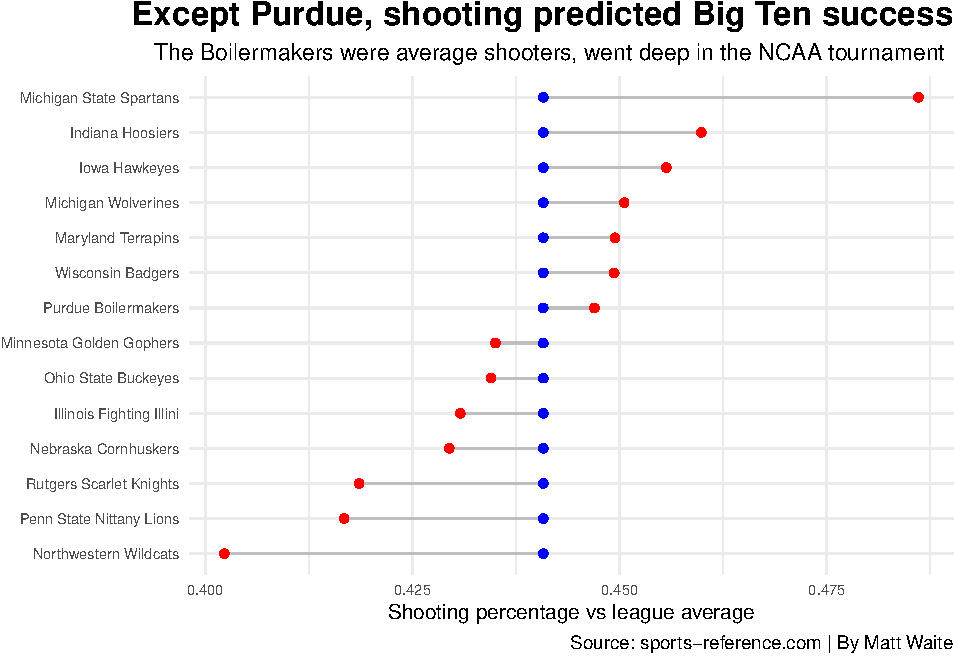
\includegraphics{SportsData_files/figure-latex/unnamed-chunk-167-1.pdf}

What if we wanted to order them by wins? Our data has a column called W\_L that lists if the team won or lost. The problem is it doens't just say W or L. If the game went to overtime, it lists that. That complicates counting wins. Here's a trick to find a string of text and make that. It's called \texttt{grepl} and the basic syntax is grepl for this string in this field and then do what I tell you. In this case, we're going to create a new field called winloss look for W or L (and ignore any OT notation) and give wins a 1 and losses a 0.

\begin{Shaded}
\begin{Highlighting}[]
\NormalTok{winlosslogs <-}\StringTok{ }\NormalTok{logs }\OperatorTok\StringTok{ }\KeywordTok{mutate}\NormalTok{(}\DataTypeTok{winloss =} \KeywordTok{case_when}\NormalTok{(}
  \KeywordTok{grepl}\NormalTok{(}\StringTok{"W"}\NormalTok{, W_L) }\OperatorTok{~}\StringTok{ }\DecValTok{1}\NormalTok{, }
  \KeywordTok{grepl}\NormalTok{(}\StringTok{"L"}\NormalTok{, W_L) }\OperatorTok{~}\StringTok{ }\DecValTok{0}\NormalTok{)}
\NormalTok{)}
\end{Highlighting}
\end{Shaded}

So let's look at turnovers and assists. We'll call it give and take. Does the difference between those two things indicate something when we sort them by wins?

\begin{Shaded}
\begin{Highlighting}[]
\NormalTok{giveandtake <-}\StringTok{ }\NormalTok{winlosslogs }\OperatorTok\StringTok{ }\KeywordTok{group_by}\NormalTok{(Conference, Team) }\OperatorTok\StringTok{ }\KeywordTok{summarise}\NormalTok{(}\DataTypeTok{turnovers =} \KeywordTok{sum}\NormalTok{(TeamTurnovers), }\DataTypeTok{assists =} \KeywordTok{sum}\NormalTok{(TeamAssists), }\DataTypeTok{wins=}\KeywordTok{sum}\NormalTok{(winloss)) }
\end{Highlighting}
\end{Shaded}

\begin{Shaded}
\begin{Highlighting}[]
\NormalTok{big10gt <-}\StringTok{ }\NormalTok{giveandtake }\OperatorTok\StringTok{ }\KeywordTok{filter}\NormalTok{(Conference }\OperatorTok{==}\StringTok{ "Big Ten"}\NormalTok{)}
\end{Highlighting}
\end{Shaded}

\begin{Shaded}
\begin{Highlighting}[]
\KeywordTok{ggplot}\NormalTok{(big10gt) }\OperatorTok{+}
\StringTok{  }\KeywordTok{geom_segment}\NormalTok{(}\KeywordTok{aes}\NormalTok{(}\DataTypeTok{x=}\KeywordTok{reorder}\NormalTok{(Team, wins), }\DataTypeTok{xend=}\NormalTok{Team, }\DataTypeTok{y=}\NormalTok{turnovers, }\DataTypeTok{yend=}\NormalTok{assists), }\DataTypeTok{color=}\StringTok{"grey"}\NormalTok{) }\OperatorTok{+}\StringTok{ }
\StringTok{  }\KeywordTok{geom_point}\NormalTok{(}\KeywordTok{aes}\NormalTok{(}\DataTypeTok{x=}\KeywordTok{reorder}\NormalTok{(Team, wins), }\DataTypeTok{y=}\NormalTok{turnovers), }\DataTypeTok{color=}\StringTok{"red"}\NormalTok{) }\OperatorTok{+}\StringTok{ }
\StringTok{  }\KeywordTok{geom_point}\NormalTok{(}\KeywordTok{aes}\NormalTok{(}\DataTypeTok{x=}\KeywordTok{reorder}\NormalTok{(Team, wins), }\DataTypeTok{y=}\NormalTok{assists), }\DataTypeTok{color=}\StringTok{"blue"}\NormalTok{) }\OperatorTok{+}
\StringTok{  }\KeywordTok{coord_flip}\NormalTok{()}
\end{Highlighting}
\end{Shaded}

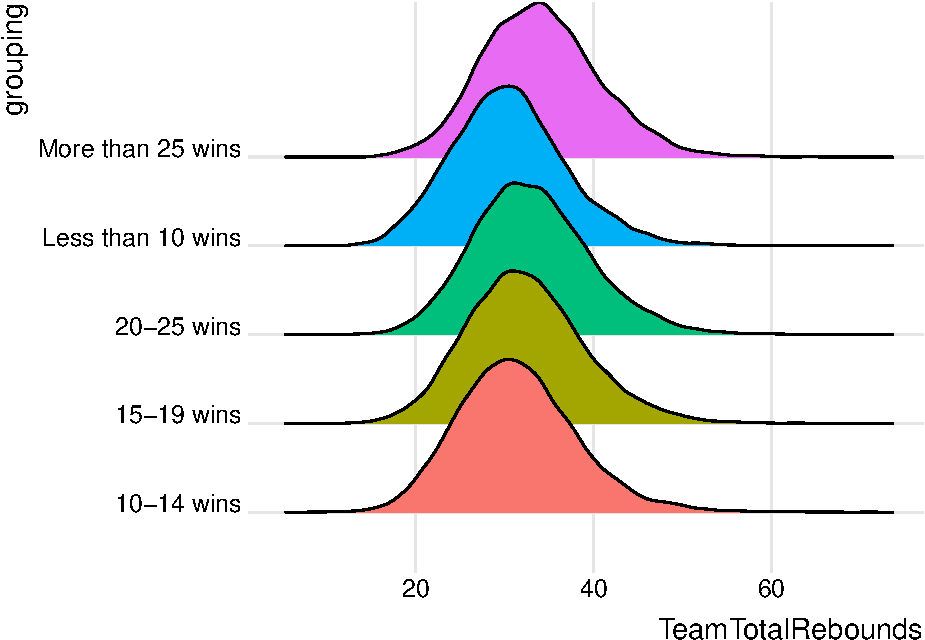
\includegraphics{SportsData_files/figure-latex/unnamed-chunk-171-1.pdf}

Short answer: Not really. Something you need to get used to in data visualization -- not everything works. Sometimes you find things, sometimes you don't. Don't publish a graphic that doesn't find anything. Let it stay in your notebook as an idea that didn't pan out.

\hypertarget{scatterplots}{%
\chapter{Scatterplots}\label{scatterplots}}

In several chapters of this book, we've been fixated on the Nebraska basketball team's shooting percentage, which took a nose dive during the season and ultimately doomed Tim Miles job. The question is \ldots{} does it matter?

This is what we're going to start to answer today. And we'll do it with scatterplots and correlations.

First, we need libraries and \href{https://unl.box.com/s/a8m91bro10t89watsyo13yjegb1fy009}{data}.

\begin{Shaded}
\begin{Highlighting}[]
\KeywordTok{library}\NormalTok{(tidyverse)}
\end{Highlighting}
\end{Shaded}

\begin{Shaded}
\begin{Highlighting}[]
\NormalTok{logs <-}\StringTok{ }\KeywordTok{read_csv}\NormalTok{(}\StringTok{"data/logs19.csv"}\NormalTok{)}
\end{Highlighting}
\end{Shaded}

\begin{verbatim}
## Warning: Missing column names filled in: 'X1' [1]
\end{verbatim}

\begin{verbatim}
## Parsed with column specification:
## cols(
##   .default = col_double(),
##   Date = col_date(format = ""),
##   HomeAway = col_character(),
##   Opponent = col_character(),
##   W_L = col_character(),
##   Blank = col_logical(),
##   Team = col_character(),
##   Conference = col_character(),
##   season = col_character()
## )
\end{verbatim}

\begin{verbatim}
## See spec(...) for full column specifications.
\end{verbatim}

To do this, we need all teams and their season stats. How much, over the course of a season, does a thing matter? That's the question you're going to answer.

In our case, we want to know how much does shooting percentage influence wins? How much difference can we explain in wins with shooting percentage? We're going to total up the number of wins each team has and their season shooting percentage in one swoop.

Let's borrow from our ridgecharts work to get the correct wins and losses totals for each team.

\begin{Shaded}
\begin{Highlighting}[]
\NormalTok{winlosslogs <-}\StringTok{ }\NormalTok{logs }\OperatorTok\StringTok{ }\KeywordTok{mutate}\NormalTok{(}\DataTypeTok{winloss =} \KeywordTok{case_when}\NormalTok{(}
  \KeywordTok{grepl}\NormalTok{(}\StringTok{"W"}\NormalTok{, W_L) }\OperatorTok{~}\StringTok{ }\DecValTok{1}\NormalTok{, }
  \KeywordTok{grepl}\NormalTok{(}\StringTok{"L"}\NormalTok{, W_L) }\OperatorTok{~}\StringTok{ }\DecValTok{0}\NormalTok{)}
\NormalTok{)}
\end{Highlighting}
\end{Shaded}

Now we can get a dataframe together that gives us the total wins for each team, and the total shots taken and made, which let's us calculate a season shooting percentage.

\begin{Shaded}
\begin{Highlighting}[]
\NormalTok{winlosslogs }\OperatorTok\StringTok{ }
\StringTok{  }\KeywordTok{group_by}\NormalTok{(Team) }\OperatorTok
\StringTok{  }\KeywordTok{summarise}\NormalTok{(}
    \DataTypeTok{wins =} \KeywordTok{sum}\NormalTok{(winloss),}
    \DataTypeTok{totalFGAttempts =} \KeywordTok{sum}\NormalTok{(TeamFGA),}
    \DataTypeTok{totalFG =} \KeywordTok{sum}\NormalTok{(TeamFG)}
\NormalTok{  ) }\OperatorTok
\StringTok{  }\KeywordTok{mutate}\NormalTok{(}\DataTypeTok{fgpct =}\NormalTok{ totalFG}\OperatorTok{/}\NormalTok{totalFGAttempts) ->}\StringTok{ }\NormalTok{fgmodel}
\end{Highlighting}
\end{Shaded}

Now let's look at the scatterplot. With a scatterplot, we put what predicts the thing on the X axis, and the thing being predicted on the Y axis. In this case, X is our shooting percentage, y is our wins.

\begin{Shaded}
\begin{Highlighting}[]
\KeywordTok{ggplot}\NormalTok{(fgmodel, }\KeywordTok{aes}\NormalTok{(}\DataTypeTok{x=}\NormalTok{fgpct, }\DataTypeTok{y=}\NormalTok{wins)) }\OperatorTok{+}\StringTok{ }\KeywordTok{geom_point}\NormalTok{()}
\end{Highlighting}
\end{Shaded}

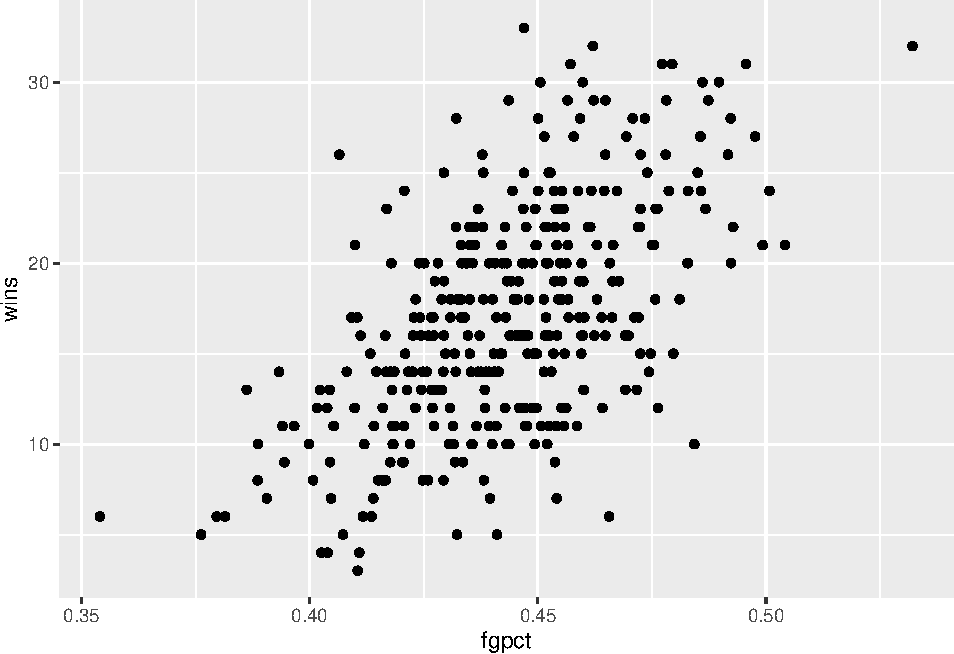
\includegraphics{SportsData_files/figure-latex/unnamed-chunk-176-1.pdf}

Let's talk about this. It seems that the data slopes up to the right. That would indicate a positive correlation between shooting percentage and wins. And that makes sense, no? You'd expect teams that shoot the ball well to win. But can we get a better sense of this? Yes, by adding another geom -- \texttt{geom\_smooth}.

\begin{Shaded}
\begin{Highlighting}[]
\KeywordTok{ggplot}\NormalTok{(fgmodel, }\KeywordTok{aes}\NormalTok{(}\DataTypeTok{x=}\NormalTok{fgpct, }\DataTypeTok{y=}\NormalTok{wins)) }\OperatorTok{+}\StringTok{ }\KeywordTok{geom_point}\NormalTok{() }\OperatorTok{+}\StringTok{ }\KeywordTok{geom_smooth}\NormalTok{(}\DataTypeTok{method=}\NormalTok{lm, }\DataTypeTok{se=}\OtherTok{TRUE}\NormalTok{)}
\end{Highlighting}
\end{Shaded}

\includegraphics{SportsData_files/figure-latex/unnamed-chunk-177-1.pdf}

But \ldots{} how strong a relationship is this? How much can shooting percentage explain wins? Can we put some numbers to this?

Of course we can. We can apply a linear model to this -- remember Chapter 9? We're going to create an object called fit, and then we're going to put into that object a linear model -- \texttt{lm} -- and the way to read this is ``wins are predicted by field goal percentage''. Then we just want the summary of that model.

\begin{Shaded}
\begin{Highlighting}[]
\NormalTok{fit <-}\StringTok{ }\KeywordTok{lm}\NormalTok{(wins }\OperatorTok{~}\StringTok{ }\NormalTok{fgpct, }\DataTypeTok{data =}\NormalTok{ fgmodel)}
\KeywordTok{summary}\NormalTok{(fit)}
\end{Highlighting}
\end{Shaded}

\begin{verbatim}
## 
## Call:
## lm(formula = wins ~ fgpct, data = fgmodel)
## 
## Residuals:
##      Min       1Q   Median       3Q      Max 
## -14.3536  -3.4523  -0.1125   3.3834  15.4318 
## 
## Coefficients:
##             Estimate Std. Error t value Pr(>|t|)    
## (Intercept)  -49.217      4.845  -10.16   <2e-16 ***
## fgpct        149.416     10.915   13.69   <2e-16 ***
## ---
## Signif. codes:  0 '***' 0.001 '**' 0.01 '*' 0.05 '.' 0.1 ' ' 1
## 
## Residual standard error: 5.035 on 351 degrees of freedom
## Multiple R-squared:  0.348,  Adjusted R-squared:  0.3462 
## F-statistic: 187.4 on 1 and 351 DF,  p-value: < 2.2e-16
\end{verbatim}

Remember from Chapter 9: There's just a few things you really need.

The first thing: R-squared. In this case, the Adjusted R-squared value is .3462, which we can interpret as shooting percentage predicts about 35 percent of the variance in wins. Which sounds not great, but in social science, that's huge. That's great. A psychology major would murder for that R-squared.

Second: The P-value. We want anything less than .05. If it's above .05, the change between them is not statistically significant -- it's probably explained by random chance. In our case, we have 2.2e-16, which is to say 2.2 with 16 zeros in front of it, or .000000000000000022. Is that less than .05? Yes. Yes it is. So this is not random. Again, we would expect this, so it's a good logic test.

Third: The coefficient. In this case, the coefficient for fgpct is 149.416. Since I didn't convert percentages to decimals, what this says is that for every percentage point improvement in shooting percentage, we can expect the team to win 1.49 more games plus or minus some error.

And we can use this to predict a team's wins: remember your algebra and y = mx + b. In this case, y is the wins, m is the coefficient, x is the shooting percentage and b is the intercept.

So can plug these together: Expected wins = 149.416 * shooting percentage - 49.217

Let's use Nebraska as an example. They shot about .43 on the season (.4294421 to be exact).

y = 149.416 * .4294421 - 49.217 or 14.95 wins. How many wins did Nebraska have? 19.

What does that mean? It means that as disappointing a season as it was, Nebraska actually OVERPERFORMED it's season shooting percentage. They shouldn't have won as many games as they did, according to our model.

\hypertarget{facet-wraps}{%
\chapter{Facet wraps}\label{facet-wraps}}

Sometimes the easiest way to spot a trend is to chart a bunch of small things side by side. Edward Tufte, one of the most well known data visualization thinkers on the planet, calls this ``small multiples'' where ggplot calls this a facet wrap or a facet grid, depending.

One thing we noticed earlier in the semester -- it seems that a lot of teams shoot worse as the season goes on. Do they? We could answer this a number of ways, but the best way to show people would be visually. Let's use Small Multiples.

As always, we start with libraries.

\begin{Shaded}
\begin{Highlighting}[]
\KeywordTok{library}\NormalTok{(tidyverse)}
\end{Highlighting}
\end{Shaded}

Now data.

\begin{Shaded}
\begin{Highlighting}[]
\NormalTok{logs <-}\StringTok{ }\KeywordTok{read_csv}\NormalTok{(}\StringTok{"data/logs19.csv"}\NormalTok{)}
\end{Highlighting}
\end{Shaded}

\begin{verbatim}
## Warning: Missing column names filled in: 'X1' [1]
\end{verbatim}

\begin{verbatim}
## Parsed with column specification:
## cols(
##   .default = col_double(),
##   Date = col_date(format = ""),
##   HomeAway = col_character(),
##   Opponent = col_character(),
##   W_L = col_character(),
##   Blank = col_logical(),
##   Team = col_character(),
##   Conference = col_character(),
##   season = col_character()
## )
\end{verbatim}

\begin{verbatim}
## See spec(...) for full column specifications.
\end{verbatim}

Let's narrow our pile and look just at the Big Ten.

\begin{Shaded}
\begin{Highlighting}[]
\NormalTok{big10 <-}\StringTok{ }\NormalTok{logs }\OperatorTok\StringTok{ }\KeywordTok{filter}\NormalTok{(Conference }\OperatorTok{==}\StringTok{ "Big Ten"}\NormalTok{)}
\end{Highlighting}
\end{Shaded}

The first thing we can do is look at a line chart, like we have done in previous chapters.

\begin{Shaded}
\begin{Highlighting}[]
\KeywordTok{ggplot}\NormalTok{() }\OperatorTok{+}\StringTok{ }\KeywordTok{geom_line}\NormalTok{(}\DataTypeTok{data=}\NormalTok{big10, }\KeywordTok{aes}\NormalTok{(}\DataTypeTok{x=}\NormalTok{Date, }\DataTypeTok{y=}\NormalTok{TeamFGPCT, }\DataTypeTok{group=}\NormalTok{Team)) }\OperatorTok{+}\StringTok{ }\KeywordTok{scale_y_continuous}\NormalTok{(}\DataTypeTok{limits =} \KeywordTok{c}\NormalTok{(}\DecValTok{0}\NormalTok{, }\FloatTok{.7}\NormalTok{))}
\end{Highlighting}
\end{Shaded}

\includegraphics{SportsData_files/figure-latex/unnamed-chunk-182-1.pdf}

And, not surprisingly, we get a hairball. We could color certain lines, but that would limit us to focus on one team. What if we did all of them at once? We do that with a \texttt{facet\_wrap}. The only thing we MUST pass into a \texttt{facet\_wrap} is what thing we're going to separate them out by. In this case, we precede that field with a tilde, so in our case we want the Team field. It looks like this:

\begin{Shaded}
\begin{Highlighting}[]
\KeywordTok{ggplot}\NormalTok{() }\OperatorTok{+}\StringTok{ }\KeywordTok{geom_line}\NormalTok{(}\DataTypeTok{data=}\NormalTok{big10, }\KeywordTok{aes}\NormalTok{(}\DataTypeTok{x=}\NormalTok{Date, }\DataTypeTok{y=}\NormalTok{TeamFGPCT, }\DataTypeTok{group=}\NormalTok{Team)) }\OperatorTok{+}\StringTok{ }\KeywordTok{scale_y_continuous}\NormalTok{(}\DataTypeTok{limits =} \KeywordTok{c}\NormalTok{(}\DecValTok{0}\NormalTok{, }\FloatTok{.7}\NormalTok{)) }\OperatorTok{+}\StringTok{ }\KeywordTok{facet_wrap}\NormalTok{(}\OperatorTok{~}\NormalTok{Team)}
\end{Highlighting}
\end{Shaded}

\includegraphics{SportsData_files/figure-latex/unnamed-chunk-183-1.pdf}

Answer: Not immediately clear, but we can look at this and analyze it. We could add a piece of annotation to help us out.

\begin{Shaded}
\begin{Highlighting}[]
\NormalTok{big10 }\OperatorTok\StringTok{ }\KeywordTok{summarise}\NormalTok{(}\KeywordTok{mean}\NormalTok{(TeamFGPCT))}
\end{Highlighting}
\end{Shaded}

\begin{verbatim}
## # A tibble: 1 x 1
##   `mean(TeamFGPCT)`
##               <dbl>
## 1             0.442
\end{verbatim}

\begin{Shaded}
\begin{Highlighting}[]
\KeywordTok{ggplot}\NormalTok{() }\OperatorTok{+}\StringTok{ }\KeywordTok{geom_hline}\NormalTok{(}\DataTypeTok{yintercept=}\NormalTok{.}\DecValTok{4447}\NormalTok{, }\DataTypeTok{color=}\StringTok{"blue"}\NormalTok{) }\OperatorTok{+}\StringTok{ }\KeywordTok{geom_line}\NormalTok{(}\DataTypeTok{data=}\NormalTok{big10, }\KeywordTok{aes}\NormalTok{(}\DataTypeTok{x=}\NormalTok{Date, }\DataTypeTok{y=}\NormalTok{TeamFGPCT, }\DataTypeTok{group=}\NormalTok{Team)) }\OperatorTok{+}\StringTok{ }\KeywordTok{scale_y_continuous}\NormalTok{(}\DataTypeTok{limits =} \KeywordTok{c}\NormalTok{(}\DecValTok{0}\NormalTok{, }\FloatTok{.7}\NormalTok{)) }\OperatorTok{+}\StringTok{ }\KeywordTok{facet_wrap}\NormalTok{(}\OperatorTok{~}\NormalTok{Team)}
\end{Highlighting}
\end{Shaded}

\includegraphics{SportsData_files/figure-latex/unnamed-chunk-185-1.pdf}

What do you see here? How do teams compare? How do they change over time? I'm not asking you these questions because they're an assignment -- I'm asking because that's exactly what this chart helps answer. Your brain will immediately start making those connections.

\hypertarget{facet-grid-vs-facet-wraps}{%
\section{Facet grid vs facet wraps}\label{facet-grid-vs-facet-wraps}}

Facet grids allow us to put teams on the same plane, versus just repeating them. And we can specify that plane as vertical or horizontal. For example, here's our chart from above, but using facet\_grid to stack them.

\begin{Shaded}
\begin{Highlighting}[]
\KeywordTok{ggplot}\NormalTok{() }\OperatorTok{+}\StringTok{ }\KeywordTok{geom_hline}\NormalTok{(}\DataTypeTok{yintercept=}\NormalTok{.}\DecValTok{4447}\NormalTok{, }\DataTypeTok{color=}\StringTok{"blue"}\NormalTok{) }\OperatorTok{+}\StringTok{ }\KeywordTok{geom_line}\NormalTok{(}\DataTypeTok{data=}\NormalTok{big10, }\KeywordTok{aes}\NormalTok{(}\DataTypeTok{x=}\NormalTok{Date, }\DataTypeTok{y=}\NormalTok{TeamFGPCT, }\DataTypeTok{group=}\NormalTok{Team)) }\OperatorTok{+}\StringTok{ }\KeywordTok{scale_y_continuous}\NormalTok{(}\DataTypeTok{limits =} \KeywordTok{c}\NormalTok{(}\DecValTok{0}\NormalTok{, }\FloatTok{.7}\NormalTok{)) }\OperatorTok{+}\StringTok{ }\KeywordTok{facet_grid}\NormalTok{(Team }\OperatorTok{~}\StringTok{ }\NormalTok{.)}
\end{Highlighting}
\end{Shaded}

\includegraphics{SportsData_files/figure-latex/unnamed-chunk-186-1.pdf}

And here they are next to each other:

\begin{Shaded}
\begin{Highlighting}[]
\KeywordTok{ggplot}\NormalTok{() }\OperatorTok{+}\StringTok{ }\KeywordTok{geom_hline}\NormalTok{(}\DataTypeTok{yintercept=}\NormalTok{.}\DecValTok{4447}\NormalTok{, }\DataTypeTok{color=}\StringTok{"blue"}\NormalTok{) }\OperatorTok{+}\StringTok{ }\KeywordTok{geom_line}\NormalTok{(}\DataTypeTok{data=}\NormalTok{big10, }\KeywordTok{aes}\NormalTok{(}\DataTypeTok{x=}\NormalTok{Date, }\DataTypeTok{y=}\NormalTok{TeamFGPCT, }\DataTypeTok{group=}\NormalTok{Team)) }\OperatorTok{+}\StringTok{ }\KeywordTok{scale_y_continuous}\NormalTok{(}\DataTypeTok{limits =} \KeywordTok{c}\NormalTok{(}\DecValTok{0}\NormalTok{, }\FloatTok{.7}\NormalTok{)) }\OperatorTok{+}\StringTok{ }\KeywordTok{facet_grid}\NormalTok{(. }\OperatorTok{~}\StringTok{ }\NormalTok{Team)}
\end{Highlighting}
\end{Shaded}

\includegraphics{SportsData_files/figure-latex/unnamed-chunk-187-1.pdf}

Note: We'd have some work to do with the labeling on this -- we'll get to that -- but you can see where this is valuable comparing a group of things. One warning: Don't go too crazy with this or it loses it's visual power.

\hypertarget{other-types}{%
\section{Other types}\label{other-types}}

Line charts aren't the only things we can do. We can do any kind of chart in ggplot. Staying with shooting, where are team's winning and losing performances coming from when we talk about team shooting and opponent shooting?

\begin{Shaded}
\begin{Highlighting}[]
\KeywordTok{ggplot}\NormalTok{() }\OperatorTok{+}\StringTok{ }\KeywordTok{geom_point}\NormalTok{(}\DataTypeTok{data=}\NormalTok{big10, }\KeywordTok{aes}\NormalTok{(}\DataTypeTok{x=}\NormalTok{TeamFGPCT, }\DataTypeTok{y=}\NormalTok{OpponentFGPCT, }\DataTypeTok{color=}\NormalTok{W_L)) }\OperatorTok{+}\StringTok{ }\KeywordTok{scale_y_continuous}\NormalTok{(}\DataTypeTok{limits =} \KeywordTok{c}\NormalTok{(}\DecValTok{0}\NormalTok{, }\FloatTok{.7}\NormalTok{)) }\OperatorTok{+}\StringTok{ }\KeywordTok{scale_x_continuous}\NormalTok{(}\DataTypeTok{limits =} \KeywordTok{c}\NormalTok{(}\DecValTok{0}\NormalTok{, }\FloatTok{.7}\NormalTok{)) }\OperatorTok{+}\StringTok{ }\KeywordTok{facet_wrap}\NormalTok{(}\OperatorTok{~}\NormalTok{Team)}
\end{Highlighting}
\end{Shaded}

\includegraphics{SportsData_files/figure-latex/unnamed-chunk-188-1.pdf}

\hypertarget{tables}{%
\chapter{Tables}\label{tables}}

But not a table. A table with features.

Sometimes, the best way to show your data is with a table -- simple rows and columns. It allows a reader to compare whatever they want to compare a little easier than a graph where you've chosen what to highlight. R has a neat package called \texttt{kableExtra}.

For this assignment, we're going to need a bunch of new libraries. Go over to the console and run these:

\begin{verbatim}
install.packages("kableExtra")
install.packages("formattable")
install.packages("htmltools")
install.packages("webshot")
webshot::install_phantomjs()
\end{verbatim}

So what does all of these libraries do? Let's gather a few and \href{https://unl.box.com/s/g3eeuogx8bog72ig28enuakhpdlbn394}{get some data}.

\begin{Shaded}
\begin{Highlighting}[]
\KeywordTok{library}\NormalTok{(tidyverse)}
\KeywordTok{library}\NormalTok{(kableExtra)}
\end{Highlighting}
\end{Shaded}

\begin{Shaded}
\begin{Highlighting}[]
\NormalTok{offense <-}\StringTok{ }\KeywordTok{read_csv}\NormalTok{(}\StringTok{"data/offensechange.csv"}\NormalTok{)}
\end{Highlighting}
\end{Shaded}

\begin{verbatim}
## Parsed with column specification:
## cols(
##   Year = col_double(),
##   Name = col_character(),
##   G = col_double(),
##   `Rush Yards` = col_double(),
##   `Pass Yards` = col_double(),
##   Plays = col_double(),
##   `Total Yards` = col_double(),
##   `Yards/Play` = col_double(),
##   `Yards/G` = col_double()
## )
\end{verbatim}

Let's ask this question: Which college football team saw the greatest improvement in yards per game last regular season? The simplest way to calculate that is by percent change.

\begin{Shaded}
\begin{Highlighting}[]
\NormalTok{changeTotalOffense <-}\StringTok{ }\NormalTok{offense }\OperatorTok
\StringTok{  }\KeywordTok{select}\NormalTok{(Name, Year, }\StringTok{`}\DataTypeTok{Yards/G}\StringTok{`}\NormalTok{) }\OperatorTok\StringTok{ }\CommentTok{# picking what we need.}
\StringTok{  }\KeywordTok{pivot_wider}\NormalTok{(}\DataTypeTok{names_from =}\NormalTok{ Year, }\DataTypeTok{values_from =} \StringTok{`}\DataTypeTok{Yards/G}\StringTok{`}\NormalTok{) }\OperatorTok\StringTok{ }\CommentTok{# making it wide }
\StringTok{  }\KeywordTok{mutate}\NormalTok{(}\DataTypeTok{Change=}\NormalTok{(}\StringTok{`}\DataTypeTok{2019}\StringTok{`}\OperatorTok{-}\StringTok{`}\DataTypeTok{2018}\StringTok{`}\NormalTok{)}\OperatorTok{/}\StringTok{`}\DataTypeTok{2018}\StringTok{`}\NormalTok{) }\OperatorTok\StringTok{ }\CommentTok{# so we can calculate percent change}
\StringTok{  }\KeywordTok{arrange}\NormalTok{(}\KeywordTok{desc}\NormalTok{(Change)) }\OperatorTok\StringTok{  }
\StringTok{  }\KeywordTok{top_n}\NormalTok{(}\DecValTok{10}\NormalTok{) }\CommentTok{# just want a top 10 list}
\end{Highlighting}
\end{Shaded}

\begin{verbatim}
## Selecting by Change
\end{verbatim}

We've output tables to the screen a thousand times in this class with \texttt{head}, but kable makes them look decent with very little code.

\begin{Shaded}
\begin{Highlighting}[]
\NormalTok{changeTotalOffense }\OperatorTok\StringTok{ }\KeywordTok{kable}\NormalTok{()}
\end{Highlighting}
\end{Shaded}

Name

2019

2018

Change

Central Michigan

433.6

254.7

0.7023950

LSU

564.1

402.1

0.4028849

UTSA

344.9

247.1

0.3957912

San Jose State

427.4

323.7

0.3203584

Navy

455.8

349.3

0.3048955

Louisville

447.3

352.6

0.2685763

SMU

489.8

387.2

0.2649793

BYU

443.8

364.9

0.2162236

New Mexico

400.3

330.0

0.2130303

Charlotte

411.8

343.1

0.2002332

So there you have it. Central Michigan improved the most (but look at who came in second!). Kable has a mountain of customization options. The good news is that it works in a very familiar pattern. We'll start with default styling.

\begin{Shaded}
\begin{Highlighting}[]
\NormalTok{changeTotalOffense }\OperatorTok\StringTok{ }
\StringTok{  }\KeywordTok{kable}\NormalTok{() }\OperatorTok\StringTok{ }
\StringTok{  }\KeywordTok{kable_styling}\NormalTok{()}
\end{Highlighting}
\end{Shaded}

Name

2019

2018

Change

Central Michigan

433.6

254.7

0.7023950

LSU

564.1

402.1

0.4028849

UTSA

344.9

247.1

0.3957912

San Jose State

427.4

323.7

0.3203584

Navy

455.8

349.3

0.3048955

Louisville

447.3

352.6

0.2685763

SMU

489.8

387.2

0.2649793

BYU

443.8

364.9

0.2162236

New Mexico

400.3

330.0

0.2130303

Charlotte

411.8

343.1

0.2002332

Let's do more than the defaults, which you can see are pretty decent. Let's stripe every other row with a little bit of grey, and let's smush the width of the rows.

\begin{Shaded}
\begin{Highlighting}[]
\NormalTok{changeTotalOffense }\OperatorTok\StringTok{ }
\StringTok{  }\KeywordTok{kable}\NormalTok{() }\OperatorTok\StringTok{ }
\StringTok{  }\KeywordTok{kable_styling}\NormalTok{(}\DataTypeTok{bootstrap_options =} \KeywordTok{c}\NormalTok{(}\StringTok{"striped"}\NormalTok{, }\StringTok{"condensed"}\NormalTok{))}
\end{Highlighting}
\end{Shaded}

Name

2019

2018

Change

Central Michigan

433.6

254.7

0.7023950

LSU

564.1

402.1

0.4028849

UTSA

344.9

247.1

0.3957912

San Jose State

427.4

323.7

0.3203584

Navy

455.8

349.3

0.3048955

Louisville

447.3

352.6

0.2685763

SMU

489.8

387.2

0.2649793

BYU

443.8

364.9

0.2162236

New Mexico

400.3

330.0

0.2130303

Charlotte

411.8

343.1

0.2002332

Throughout the semester, we've been using color and other signals to highlight things. Let's pretend we're doing a project on LSU. We can use row\_spec to highlight things.

What row\_spec is doing here is we're specifying which row -- 2 -- and making all the text on that row bold. We're making the color of the text white, because we're going to set the background to a color -- in this case, the hex color for LSU purple.

\begin{Shaded}
\begin{Highlighting}[]
\NormalTok{changeTotalOffense }\OperatorTok\StringTok{ }
\StringTok{  }\KeywordTok{kable}\NormalTok{() }\OperatorTok\StringTok{ }
\StringTok{  }\KeywordTok{kable_styling}\NormalTok{(}\DataTypeTok{bootstrap_options =} \KeywordTok{c}\NormalTok{(}\StringTok{"striped"}\NormalTok{, }\StringTok{"condensed"}\NormalTok{)) }\OperatorTok
\StringTok{  }\KeywordTok{row_spec}\NormalTok{(}\DecValTok{2}\NormalTok{, }\DataTypeTok{bold =}\NormalTok{ T, }\DataTypeTok{color =} \StringTok{"white"}\NormalTok{, }\DataTypeTok{background =} \StringTok{"#461D7C"}\NormalTok{)}
\end{Highlighting}
\end{Shaded}

Name

2019

2018

Change

Central Michigan

433.6

254.7

0.7023950

LSU

564.1

402.1

0.4028849

UTSA

344.9

247.1

0.3957912

San Jose State

427.4

323.7

0.3203584

Navy

455.8

349.3

0.3048955

Louisville

447.3

352.6

0.2685763

SMU

489.8

387.2

0.2649793

BYU

443.8

364.9

0.2162236

New Mexico

400.3

330.0

0.2130303

Charlotte

411.8

343.1

0.2002332

There's also something called column\_spec where we can change the styling on individual columns. What if we wanted to make all the team names bold?

\begin{Shaded}
\begin{Highlighting}[]
\NormalTok{changeTotalOffense }\OperatorTok\StringTok{ }
\StringTok{  }\KeywordTok{kable}\NormalTok{() }\OperatorTok\StringTok{ }
\StringTok{  }\KeywordTok{kable_styling}\NormalTok{(}\DataTypeTok{bootstrap_options =} \KeywordTok{c}\NormalTok{(}\StringTok{"striped"}\NormalTok{, }\StringTok{"condensed"}\NormalTok{)) }\OperatorTok
\StringTok{  }\KeywordTok{row_spec}\NormalTok{(}\DecValTok{2}\NormalTok{, }\DataTypeTok{bold =}\NormalTok{ T, }\DataTypeTok{color =} \StringTok{"white"}\NormalTok{, }\DataTypeTok{background =} \StringTok{"#461D7C"}\NormalTok{) }\OperatorTok
\StringTok{  }\KeywordTok{column_spec}\NormalTok{(}\DecValTok{1}\NormalTok{, }\DataTypeTok{bold=}\NormalTok{T)}
\end{Highlighting}
\end{Shaded}

Name

2019

2018

Change

Central Michigan

433.6

254.7

0.7023950

LSU

564.1

402.1

0.4028849

UTSA

344.9

247.1

0.3957912

San Jose State

427.4

323.7

0.3203584

Navy

455.8

349.3

0.3048955

Louisville

447.3

352.6

0.2685763

SMU

489.8

387.2

0.2649793

BYU

443.8

364.9

0.2162236

New Mexico

400.3

330.0

0.2130303

Charlotte

411.8

343.1

0.2002332

Honestly, this is really good right here. You'd see this published \ldots{} except for one thing: the percentages.

We could go back up to the top and multiply by 100, but we'd still be missing the percent sign. Well, there's another library for making interesting tables that, in my opinion, has some flaws but does some interesting things too called \texttt{formattable}.

Go to the console and install \texttt{formattable} with \texttt{install.packages("formattable")}.

\begin{Shaded}
\begin{Highlighting}[]
\KeywordTok{library}\NormalTok{(formattable)}
\end{Highlighting}
\end{Shaded}

Then, we're going to use mutate here to use formattables \texttt{percent()} function to fix Change. Because it uses some HTML wizardry under the hood, we have to set kable to not \texttt{escape} the HTML.

\begin{Shaded}
\begin{Highlighting}[]
\NormalTok{changeTotalOffense }\OperatorTok\StringTok{ }
\StringTok{  }\KeywordTok{mutate}\NormalTok{(}\DataTypeTok{Change =} \KeywordTok{percent}\NormalTok{(Change)) }\OperatorTok
\StringTok{  }\KeywordTok{kable}\NormalTok{(}\DataTypeTok{escape=}\NormalTok{F) }\OperatorTok\StringTok{ }
\StringTok{  }\KeywordTok{kable_styling}\NormalTok{(}\DataTypeTok{bootstrap_options =} \KeywordTok{c}\NormalTok{(}\StringTok{"striped"}\NormalTok{, }\StringTok{"condensed"}\NormalTok{)) }\OperatorTok
\StringTok{  }\KeywordTok{row_spec}\NormalTok{(}\DecValTok{2}\NormalTok{, }\DataTypeTok{bold =}\NormalTok{ T, }\DataTypeTok{color =} \StringTok{"white"}\NormalTok{, }\DataTypeTok{background =} \StringTok{"#461D7C"}\NormalTok{) }\OperatorTok
\StringTok{  }\KeywordTok{column_spec}\NormalTok{(}\DecValTok{1}\NormalTok{, }\DataTypeTok{bold=}\NormalTok{T)}
\end{Highlighting}
\end{Shaded}

Name

2019

2018

Change

Central Michigan

433.6

254.7

70.24\%

LSU

564.1

402.1

40.29\%

UTSA

344.9

247.1

39.58\%

San Jose State

427.4

323.7

32.04\%

Navy

455.8

349.3

30.49\%

Louisville

447.3

352.6

26.86\%

SMU

489.8

387.2

26.50\%

BYU

443.8

364.9

21.62\%

New Mexico

400.3

330.0

21.30\%

Charlotte

411.8

343.1

20.02\%

Another way to highlight things: color ramps. We can change the color of the box covering the percentage using another mutate like this:

\begin{Shaded}
\begin{Highlighting}[]
\NormalTok{changeTotalOffense }\OperatorTok\StringTok{ }
\StringTok{  }\KeywordTok{mutate}\NormalTok{(}\DataTypeTok{Change =} \KeywordTok{percent}\NormalTok{(Change)) }\OperatorTok
\StringTok{  }\KeywordTok{mutate}\NormalTok{(}\DataTypeTok{Change =} \KeywordTok{cell_spec}\NormalTok{(}
\NormalTok{    Change, }\DataTypeTok{color =} \StringTok{"white"}\NormalTok{, }\DataTypeTok{bold =}\NormalTok{ T,}
    \DataTypeTok{background =} \KeywordTok{spec_color}\NormalTok{(}\DecValTok{1}\OperatorTok{:}\DecValTok{10}\NormalTok{, }\DataTypeTok{end =} \FloatTok{0.75}\NormalTok{, }\DataTypeTok{option =} \StringTok{"B"}\NormalTok{, }\DataTypeTok{direction =} \DecValTok{-1}\NormalTok{)}
\NormalTok{  )) }\OperatorTok
\StringTok{  }\KeywordTok{kable}\NormalTok{(}\DataTypeTok{escape=}\NormalTok{F) }\OperatorTok\StringTok{ }
\StringTok{  }\KeywordTok{kable_styling}\NormalTok{(}\DataTypeTok{bootstrap_options =} \KeywordTok{c}\NormalTok{(}\StringTok{"striped"}\NormalTok{, }\StringTok{"condensed"}\NormalTok{)) }\OperatorTok
\StringTok{  }\KeywordTok{row_spec}\NormalTok{(}\DecValTok{2}\NormalTok{, }\DataTypeTok{bold =}\NormalTok{ T, }\DataTypeTok{color =} \StringTok{"white"}\NormalTok{, }\DataTypeTok{background =} \StringTok{"#461D7C"}\NormalTok{) }\OperatorTok
\StringTok{  }\KeywordTok{column_spec}\NormalTok{(}\DecValTok{1}\NormalTok{, }\DataTypeTok{bold=}\NormalTok{T)}
\end{Highlighting}
\end{Shaded}

Name

2019

2018

Change

Central Michigan

433.6

254.7

{70.24\%}

LSU

564.1

402.1

{40.29\%}

UTSA

344.9

247.1

{39.58\%}

San Jose State

427.4

323.7

{32.04\%}

Navy

455.8

349.3

{30.49\%}

Louisville

447.3

352.6

{26.86\%}

SMU

489.8

387.2

{26.50\%}

BYU

443.8

364.9

{21.62\%}

New Mexico

400.3

330.0

{21.30\%}

Charlotte

411.8

343.1

{20.02\%}

If this is intersting to you, \href{https://cran.r-project.org/web/packages/kableExtra/vignettes/awesome_table_in_html.html\#overview}{there's more you can do}.

\hypertarget{exporting-tables}{%
\section{Exporting tables}\label{exporting-tables}}

One of the major shortcomings with \texttt{formattable} is a very limited ability to export tables. Fortunately, \texttt{kable} appears to have solved that problem.

But, for this to be a finished product, we need to add a headline, credit line and source line.

Good news bad news: The bad news is that \texttt{kable} doesn't have a good way to add a headline. The good news is we can do that in illustrator pretty easily.

The other good news bad news: \texttt{kable} isn't going to export this as an actual vector file. It's going to make it an image and embed that into a pdf. That has consequences if we want to edit it.

To export it, we merely add a save\_kable to the end and give it a file path.

\begin{Shaded}
\begin{Highlighting}[]
\NormalTok{changeTotalOffense }\OperatorTok\StringTok{ }
\StringTok{  }\KeywordTok{mutate}\NormalTok{(}\DataTypeTok{Change =} \KeywordTok{percent}\NormalTok{(Change)) }\OperatorTok
\StringTok{  }\KeywordTok{mutate}\NormalTok{(}\DataTypeTok{Change =} \KeywordTok{cell_spec}\NormalTok{(}
\NormalTok{    Change, }\DataTypeTok{color =} \StringTok{"white"}\NormalTok{, }\DataTypeTok{bold =}\NormalTok{ T,}
    \DataTypeTok{background =} \KeywordTok{spec_color}\NormalTok{(}\DecValTok{1}\OperatorTok{:}\DecValTok{10}\NormalTok{, }\DataTypeTok{end =} \FloatTok{0.75}\NormalTok{, }\DataTypeTok{option =} \StringTok{"B"}\NormalTok{, }\DataTypeTok{direction =} \DecValTok{-1}\NormalTok{)}
\NormalTok{  )) }\OperatorTok
\StringTok{  }\KeywordTok{kable}\NormalTok{(}\DataTypeTok{escape=}\NormalTok{F) }\OperatorTok\StringTok{ }
\StringTok{  }\KeywordTok{kable_styling}\NormalTok{(}\DataTypeTok{bootstrap_options =} \KeywordTok{c}\NormalTok{(}\StringTok{"striped"}\NormalTok{, }\StringTok{"condensed"}\NormalTok{)) }\OperatorTok
\StringTok{  }\KeywordTok{row_spec}\NormalTok{(}\DecValTok{2}\NormalTok{, }\DataTypeTok{bold =}\NormalTok{ T, }\DataTypeTok{color =} \StringTok{"white"}\NormalTok{, }\DataTypeTok{background =} \StringTok{"#461D7C"}\NormalTok{) }\OperatorTok
\StringTok{  }\KeywordTok{column_spec}\NormalTok{(}\DecValTok{1}\NormalTok{, }\DataTypeTok{bold=}\NormalTok{T) }\OperatorTok
\StringTok{  }\KeywordTok{save_kable}\NormalTok{(}\StringTok{"lsu.pdf"}\NormalTok{)}
\end{Highlighting}
\end{Shaded}

To fix this, we need to pull it into Illustrator. In there, we're going to expand the artboard, add a headline and chatter, then add source and credit lines at the bottom, and finish with touching up the artboards.

Here's a video walkthrough:

\hypertarget{bubble-charts}{%
\chapter{Bubble charts}\label{bubble-charts}}

Here is the real talk: Bubble charts are hard. The reason they are hard is not because of the code, or the complexity or anything like that. They're a scatterplot with magnitude added -- the size of the dot in the scatterplot has meaning. The hard part is seeing when a bubble chart works and when it doesn't.

If you want to see it work spectacularly well, \href{https://www.youtube.com/watch?v=hVimVzgtD6w}{watch a semi-famous Ted Talk} by Hans Rosling from 2006 where bubble charts were the centerpiece. It's worth watching. It'll change your perspective on the world. No seriously. It will.

And since then, people have wanted bubble charts. And we're back to the original problem: They're hard. There's a finite set of circumstances where they work.

First, I'm going to show you an example of them not working to illustrate the point.

I'm going to load up my libraries: tidyverse per usual, rvest to get some data (we'll discuss rvest in greater detail in an upcoming chapter) and ggrepel because I end up using it every time I do a scatterplot.

\begin{Shaded}
\begin{Highlighting}[]
\KeywordTok{library}\NormalTok{(tidyverse)}
\KeywordTok{library}\NormalTok{(rvest)}
\KeywordTok{library}\NormalTok{(ggrepel)}
\end{Highlighting}
\end{Shaded}

So for this example, I want to look at Nebraska's offense in the 2019 season. It \ldots{} hasn't gone well. And typical of Nebraska teams for the last decade, they're turning the ball over a lot. So given the number of turnovers, how does Nebraska compare to other teams in the FBS?

I'm going to create a scatterplot yards per game on the X axis and points per game on the Y. They're pretty highly correlated with each other. And then I'm going to make the dot the size of the turnovers -- the bubble in my bubble charts.

Using Rvest, I'm going to grab total offense rankings, scoring offense rankings and turnover rankings and then merge them together with just the fields I need. This will all get explained more thoroughly coming up, but that's what this block of code does. When it's done, I'll have a dataframe called \texttt{offense} which I'll use to build my bubble chart.

\begin{Shaded}
\begin{Highlighting}[]
\NormalTok{yardsurl <-}\StringTok{ "http://cfbstats.com/2019/leader/national/team/offense/split01/category10/sort01.html"}

\NormalTok{yards19 <-}\StringTok{ }\NormalTok{yardsurl }\OperatorTok
\StringTok{  }\KeywordTok{read_html}\NormalTok{() }\OperatorTok
\StringTok{  }\KeywordTok{html_nodes}\NormalTok{(}\DataTypeTok{xpath =} \StringTok{'//*[@id="content"]/div[2]/table'}\NormalTok{) }\OperatorTok
\StringTok{  }\KeywordTok{html_table}\NormalTok{()}

\NormalTok{yards19 <-}\StringTok{ }\NormalTok{yards19[[}\DecValTok{1}\NormalTok{]] }\OperatorTok\StringTok{ }\KeywordTok{select}\NormalTok{(Name, }\StringTok{`}\DataTypeTok{Yards/G}\StringTok{`}\NormalTok{)}

\NormalTok{pointsurl <-}\StringTok{ "http://cfbstats.com/2019/leader/national/team/offense/split01/category09/sort01.html"}

\NormalTok{points19 <-}\StringTok{ }\NormalTok{pointsurl }\OperatorTok
\StringTok{  }\KeywordTok{read_html}\NormalTok{() }\OperatorTok
\StringTok{  }\KeywordTok{html_nodes}\NormalTok{(}\DataTypeTok{xpath =} \StringTok{'//*[@id="content"]/div[2]/table'}\NormalTok{) }\OperatorTok
\StringTok{  }\KeywordTok{html_table}\NormalTok{()}

\NormalTok{points19 <-}\StringTok{ }\NormalTok{points19[[}\DecValTok{1}\NormalTok{]] }\OperatorTok\StringTok{ }\KeywordTok{select}\NormalTok{(Name, }\StringTok{`}\DataTypeTok{Points/G}\StringTok{`}\NormalTok{)}

\NormalTok{turnoversurl <-}\StringTok{ "http://cfbstats.com/2019/leader/national/team/offense/split01/category12/sort01.html"}

\NormalTok{turnovers19 <-}\StringTok{ }\NormalTok{turnoversurl }\OperatorTok
\StringTok{  }\KeywordTok{read_html}\NormalTok{() }\OperatorTok
\StringTok{  }\KeywordTok{html_nodes}\NormalTok{(}\DataTypeTok{xpath =} \StringTok{'//*[@id="content"]/div[2]/table'}\NormalTok{) }\OperatorTok
\StringTok{  }\KeywordTok{html_table}\NormalTok{()}

\NormalTok{turnovers19 <-}\StringTok{ }\NormalTok{turnovers19[[}\DecValTok{1}\NormalTok{]] }\OperatorTok\StringTok{ }\KeywordTok{select}\NormalTok{(Name, }\StringTok{`}\DataTypeTok{Total Lost}\StringTok{`}\NormalTok{)}


\NormalTok{offense <-}\StringTok{ }\NormalTok{yards19 }\OperatorTok
\StringTok{  }\KeywordTok{left_join}\NormalTok{(points19, }\DataTypeTok{by=}\KeywordTok{c}\NormalTok{(}\StringTok{"Name"}\NormalTok{)) }\OperatorTok
\StringTok{  }\KeywordTok{left_join}\NormalTok{(turnovers19, }\DataTypeTok{by=}\KeywordTok{c}\NormalTok{(}\StringTok{"Name"}\NormalTok{))}
\end{Highlighting}
\end{Shaded}

A bubble chart is just a scatterplot with one additional element in the aesthetic -- a size. Here's the scatterplot version.

\begin{Shaded}
\begin{Highlighting}[]
\KeywordTok{ggplot}\NormalTok{() }\OperatorTok{+}\StringTok{ }\KeywordTok{geom_point}\NormalTok{(}\DataTypeTok{data=}\NormalTok{offense, }\KeywordTok{aes}\NormalTok{(}\DataTypeTok{x=}\StringTok{`}\DataTypeTok{Yards/G}\StringTok{`}\NormalTok{, }\DataTypeTok{y=}\StringTok{`}\DataTypeTok{Points/G}\StringTok{`}\NormalTok{))}
\end{Highlighting}
\end{Shaded}

\includegraphics{SportsData_files/figure-latex/unnamed-chunk-203-1.pdf}

As expected, yards per game pretty tightly predicts points per game, but you could have guessed that without a chart. So let's add the size element.

\begin{Shaded}
\begin{Highlighting}[]
\KeywordTok{ggplot}\NormalTok{() }\OperatorTok{+}\StringTok{ }\KeywordTok{geom_point}\NormalTok{(}\DataTypeTok{data=}\NormalTok{offense, }\KeywordTok{aes}\NormalTok{(}\DataTypeTok{x=}\StringTok{`}\DataTypeTok{Yards/G}\StringTok{`}\NormalTok{, }\DataTypeTok{y=}\StringTok{`}\DataTypeTok{Points/G}\StringTok{`}\NormalTok{, }\DataTypeTok{size=}\StringTok{`}\DataTypeTok{Total Lost}\StringTok{`}\NormalTok{)) }
\end{Highlighting}
\end{Shaded}

\includegraphics{SportsData_files/figure-latex/unnamed-chunk-204-1.pdf}

Eh. What does this chart tell you? Trick question, there's not much new here. The dots are too big. Also, we can't see when they overlap. We can fix that by adding an alpha element outside the aesthetic -- alpha in this case is transparency -- and we can manually change the size of the dots by adding \texttt{scale\_size} and a \texttt{range}.

\begin{Shaded}
\begin{Highlighting}[]
\KeywordTok{ggplot}\NormalTok{() }\OperatorTok{+}\StringTok{ }\KeywordTok{geom_point}\NormalTok{(}\DataTypeTok{data=}\NormalTok{offense, }\KeywordTok{aes}\NormalTok{(}\DataTypeTok{x=}\StringTok{`}\DataTypeTok{Yards/G}\StringTok{`}\NormalTok{, }\DataTypeTok{y=}\StringTok{`}\DataTypeTok{Points/G}\StringTok{`}\NormalTok{, }\DataTypeTok{size=}\StringTok{`}\DataTypeTok{Total Lost}\StringTok{`}\NormalTok{), }\DataTypeTok{alpha=}\NormalTok{.}\DecValTok{2}\NormalTok{) }\OperatorTok{+}\StringTok{ }\KeywordTok{scale_size}\NormalTok{(}\DataTypeTok{range =} \KeywordTok{c}\NormalTok{(.}\DecValTok{1}\NormalTok{, }\DecValTok{15}\NormalTok{), }\DataTypeTok{name=}\StringTok{"Turnovers"}\NormalTok{)}
\end{Highlighting}
\end{Shaded}

\includegraphics{SportsData_files/figure-latex/unnamed-chunk-205-1.pdf}

Before we do any more work, let's return to the earlier question: What story does this tell? Can you discern a story from the bubbles? Are teams with lots of turnovers doing poorly and teams with few turnovers doing well? The problem is, you can't really tell. So this is a dead end for a bubble chart. If you get a big mess, it's a dead giveaway that you probably don't have a bubble chart.

So let's look at something else. Let's look at something that isn't directly correlated -- we'll look at offensive points per game vs defensive points per game.

I'm going to edit the same rvest code to grab those points per game stats and merge it all together. When it's done, I'll have a dataframe called \texttt{football} and we can look at where good teams fall on the chart with turnover margin as a scaled dot.

\begin{Shaded}
\begin{Highlighting}[]
\NormalTok{ourl <-}\StringTok{ "http://cfbstats.com/2019/leader/national/team/offense/split01/category09/sort01.html"}

\NormalTok{o19 <-}\StringTok{ }\NormalTok{ourl }\OperatorTok
\StringTok{  }\KeywordTok{read_html}\NormalTok{() }\OperatorTok
\StringTok{  }\KeywordTok{html_nodes}\NormalTok{(}\DataTypeTok{xpath =} \StringTok{'//*[@id="content"]/div[2]/table'}\NormalTok{) }\OperatorTok
\StringTok{  }\KeywordTok{html_table}\NormalTok{()}

\NormalTok{o19 <-}\StringTok{ }\NormalTok{o19[[}\DecValTok{1}\NormalTok{]] }\OperatorTok\StringTok{ }\KeywordTok{select}\NormalTok{(Name, }\StringTok{`}\DataTypeTok{Points/G}\StringTok{`}\NormalTok{)}

\NormalTok{durl <-}\StringTok{ "http://cfbstats.com/2019/leader/national/team/defense/split01/category09/sort01.html"}

\NormalTok{d19 <-}\StringTok{ }\NormalTok{durl }\OperatorTok
\StringTok{  }\KeywordTok{read_html}\NormalTok{() }\OperatorTok
\StringTok{  }\KeywordTok{html_nodes}\NormalTok{(}\DataTypeTok{xpath =} \StringTok{'//*[@id="content"]/div[2]/table'}\NormalTok{) }\OperatorTok
\StringTok{  }\KeywordTok{html_table}\NormalTok{()}

\NormalTok{d19 <-}\StringTok{ }\NormalTok{d19[[}\DecValTok{1}\NormalTok{]] }\OperatorTok\StringTok{ }\KeywordTok{select}\NormalTok{(Name, }\StringTok{`}\DataTypeTok{Points/G}\StringTok{`}\NormalTok{)}

\NormalTok{turnoversurl <-}\StringTok{ "http://cfbstats.com/2019/leader/national/team/offense/split01/category12/sort01.html"}

\NormalTok{turnovers19 <-}\StringTok{ }\NormalTok{turnoversurl }\OperatorTok
\StringTok{  }\KeywordTok{read_html}\NormalTok{() }\OperatorTok
\StringTok{  }\KeywordTok{html_nodes}\NormalTok{(}\DataTypeTok{xpath =} \StringTok{'//*[@id="content"]/div[2]/table'}\NormalTok{) }\OperatorTok
\StringTok{  }\KeywordTok{html_table}\NormalTok{()}

\NormalTok{turnovers19 <-}\StringTok{ }\NormalTok{turnovers19[[}\DecValTok{1}\NormalTok{]] }\OperatorTok\StringTok{ }\KeywordTok{select}\NormalTok{(Name, Margin)}

\NormalTok{football <-}\StringTok{ }\NormalTok{o19 }\OperatorTok\StringTok{ }
\StringTok{  }\KeywordTok{left_join}\NormalTok{(d19, }\DataTypeTok{by=}\KeywordTok{c}\NormalTok{(}\StringTok{"Name"}\NormalTok{)) }\OperatorTok\StringTok{ }
\StringTok{  }\KeywordTok{left_join}\NormalTok{(turnovers19, }\DataTypeTok{by=}\KeywordTok{c}\NormalTok{(}\StringTok{"Name"}\NormalTok{)) }\OperatorTok\StringTok{ }
\StringTok{  }\KeywordTok{rename}\NormalTok{(}\StringTok{`}\DataTypeTok{Offensive Points Per Game}\StringTok{`}\NormalTok{ =}\StringTok{ `}\DataTypeTok{Points/G.x}\StringTok{`}\NormalTok{, }\StringTok{`}\DataTypeTok{Defensive Points Per Game}\StringTok{`}\NormalTok{=}\StringTok{`}\DataTypeTok{Points/G.y}\StringTok{`}\NormalTok{)}
\end{Highlighting}
\end{Shaded}

Now we can do the bubble chart.

\begin{Shaded}
\begin{Highlighting}[]
\KeywordTok{ggplot}\NormalTok{() }\OperatorTok{+}\StringTok{ }\KeywordTok{geom_point}\NormalTok{(}\DataTypeTok{data=}\NormalTok{football, }\KeywordTok{aes}\NormalTok{(}\DataTypeTok{x=}\StringTok{`}\DataTypeTok{Offensive Points Per Game}\StringTok{`}\NormalTok{, }\DataTypeTok{y=}\StringTok{`}\DataTypeTok{Defensive Points Per Game}\StringTok{`}\NormalTok{, }\DataTypeTok{size=}\NormalTok{Margin), }\DataTypeTok{alpha=}\NormalTok{.}\DecValTok{2}\NormalTok{) }\OperatorTok{+}\StringTok{ }\KeywordTok{scale_size}\NormalTok{(}\DataTypeTok{range =} \KeywordTok{c}\NormalTok{(}\DecValTok{0}\NormalTok{, }\DecValTok{6}\NormalTok{), }\DataTypeTok{name=}\StringTok{"Turnovers"}\NormalTok{)}
\end{Highlighting}
\end{Shaded}

\includegraphics{SportsData_files/figure-latex/unnamed-chunk-207-1.pdf}

Better! Teams are spread out a little more. Bottom right quadrant -- the good defense, good offense quadrant -- have some large dots. The upper left quadrant -- bad defense, bad offense -- have some very small dots, meaning they have a really terrible turnover margin.

But what would make this chart better -- and what you saw in the Rosling video -- is color. What if we colored the dots by if they were above or below zero? Meaning, do they have a positive or negative turnover margin? We can do that with a quick mutate and a case\_when statement.

\begin{Shaded}
\begin{Highlighting}[]
\NormalTok{football <-}\StringTok{ }\NormalTok{football }\OperatorTok\StringTok{ }\KeywordTok{mutate}\NormalTok{(}\DataTypeTok{PositiveNegative =} \KeywordTok{case_when}\NormalTok{(}
\NormalTok{  Margin }\OperatorTok{>}\StringTok{ }\DecValTok{0} \OperatorTok{~}\StringTok{ "Positive"}\NormalTok{,}
\NormalTok{  Margin }\OperatorTok{<}\StringTok{ }\DecValTok{0} \OperatorTok{~}\StringTok{ "Negative"}\NormalTok{,}
\NormalTok{  Margin }\OperatorTok{==}\StringTok{ }\DecValTok{0} \OperatorTok{~}\StringTok{ "Even"}
\NormalTok{))}
\end{Highlighting}
\end{Shaded}

Now we can add \texttt{color=PositiveNegative} to the aesthetic and our dots will be colored by if they are positive, negative or zero.

\begin{Shaded}
\begin{Highlighting}[]
\KeywordTok{ggplot}\NormalTok{() }\OperatorTok{+}\StringTok{ }\KeywordTok{geom_point}\NormalTok{(}\DataTypeTok{data=}\NormalTok{football, }\KeywordTok{aes}\NormalTok{(}\DataTypeTok{x=}\StringTok{`}\DataTypeTok{Offensive Points Per Game}\StringTok{`}\NormalTok{, }\DataTypeTok{y=}\StringTok{`}\DataTypeTok{Defensive Points Per Game}\StringTok{`}\NormalTok{, }\DataTypeTok{size=}\NormalTok{Margin, }\DataTypeTok{color=}\NormalTok{PositiveNegative), }\DataTypeTok{alpha=}\NormalTok{.}\DecValTok{2}\NormalTok{) }\OperatorTok{+}\StringTok{ }\KeywordTok{scale_size}\NormalTok{(}\DataTypeTok{range =} \KeywordTok{c}\NormalTok{(}\DecValTok{0}\NormalTok{, }\DecValTok{6}\NormalTok{), }\DataTypeTok{name=}\StringTok{"Turnovers"}\NormalTok{)}
\end{Highlighting}
\end{Shaded}

\includegraphics{SportsData_files/figure-latex/unnamed-chunk-209-1.pdf}

Now we're getting somewhere. What's the story that this chart tells? Blue dots -- positive turnover margins -- are all drifting toward that good offense, good defense quadrant. Green dots -- negative turnover margins -- are drifting toward that bad defense, bad offense quadrant.

Let's add some annotations. Let's look at the top two turnover margin teams and where they come out.

\begin{Shaded}
\begin{Highlighting}[]
\NormalTok{topteams <-}\StringTok{ }\NormalTok{football }\OperatorTok\StringTok{ }\KeywordTok{filter}\NormalTok{(Name }\OperatorTok{==}\StringTok{ "LSU"} \OperatorTok{|}\StringTok{ }\NormalTok{Name }\OperatorTok{==}\StringTok{ "Alabama"}\NormalTok{)}
\end{Highlighting}
\end{Shaded}

\begin{Shaded}
\begin{Highlighting}[]
\KeywordTok{ggplot}\NormalTok{() }\OperatorTok{+}
\StringTok{  }\KeywordTok{geom_point}\NormalTok{(}\DataTypeTok{data=}\NormalTok{football, }\KeywordTok{aes}\NormalTok{(}\DataTypeTok{x=}\StringTok{`}\DataTypeTok{Offensive Points Per Game}\StringTok{`}\NormalTok{, }\DataTypeTok{y=}\StringTok{`}\DataTypeTok{Defensive Points Per Game}\StringTok{`}\NormalTok{, }\DataTypeTok{size=}\NormalTok{Margin, }\DataTypeTok{color=}\NormalTok{PositiveNegative), }\DataTypeTok{alpha=}\NormalTok{.}\DecValTok{2}\NormalTok{) }\OperatorTok{+}
\StringTok{  }\KeywordTok{geom_text_repel}\NormalTok{(}\DataTypeTok{data=}\NormalTok{topteams, }\KeywordTok{aes}\NormalTok{(}\DataTypeTok{x=}\StringTok{`}\DataTypeTok{Offensive Points Per Game}\StringTok{`}\NormalTok{, }\DataTypeTok{y=}\StringTok{`}\DataTypeTok{Defensive Points Per Game}\StringTok{`}\NormalTok{, }\DataTypeTok{label=}\NormalTok{Name)) }\OperatorTok{+}\StringTok{ }
\StringTok{  }\KeywordTok{scale_size}\NormalTok{(}\DataTypeTok{range =} \KeywordTok{c}\NormalTok{(}\DecValTok{0}\NormalTok{, }\DecValTok{6}\NormalTok{), }\DataTypeTok{name=}\StringTok{"Turnovers"}\NormalTok{)}
\end{Highlighting}
\end{Shaded}

\includegraphics{SportsData_files/figure-latex/unnamed-chunk-211-1.pdf}

No surprise there. What about Nebraska?

\begin{Shaded}
\begin{Highlighting}[]
\NormalTok{nu <-}\StringTok{ }\NormalTok{football }\OperatorTok\StringTok{ }\KeywordTok{filter}\NormalTok{(Name}\OperatorTok{==}\StringTok{"Nebraska"}\NormalTok{)}
\end{Highlighting}
\end{Shaded}

\begin{Shaded}
\begin{Highlighting}[]
\KeywordTok{ggplot}\NormalTok{() }\OperatorTok{+}
\StringTok{  }\KeywordTok{geom_point}\NormalTok{(}\DataTypeTok{data=}\NormalTok{football, }\KeywordTok{aes}\NormalTok{(}\DataTypeTok{x=}\StringTok{`}\DataTypeTok{Offensive Points Per Game}\StringTok{`}\NormalTok{, }\DataTypeTok{y=}\StringTok{`}\DataTypeTok{Defensive Points Per Game}\StringTok{`}\NormalTok{, }\DataTypeTok{size=}\NormalTok{Margin, }\DataTypeTok{color=}\NormalTok{PositiveNegative), }\DataTypeTok{alpha=}\NormalTok{.}\DecValTok{2}\NormalTok{) }\OperatorTok{+}
\StringTok{  }\KeywordTok{geom_text_repel}\NormalTok{(}\DataTypeTok{data=}\NormalTok{topteams, }\KeywordTok{aes}\NormalTok{(}\DataTypeTok{x=}\StringTok{`}\DataTypeTok{Offensive Points Per Game}\StringTok{`}\NormalTok{, }\DataTypeTok{y=}\StringTok{`}\DataTypeTok{Defensive Points Per Game}\StringTok{`}\NormalTok{, }\DataTypeTok{label=}\NormalTok{Name)) }\OperatorTok{+}\StringTok{ }
\StringTok{  }\KeywordTok{geom_point}\NormalTok{(}\DataTypeTok{data=}\NormalTok{nu, }\KeywordTok{aes}\NormalTok{(}\DataTypeTok{x=}\StringTok{`}\DataTypeTok{Offensive Points Per Game}\StringTok{`}\NormalTok{, }\DataTypeTok{y=}\StringTok{`}\DataTypeTok{Defensive Points Per Game}\StringTok{`}\NormalTok{, }\DataTypeTok{size=}\NormalTok{Margin), }\DataTypeTok{alpha=}\NormalTok{.}\DecValTok{2}\NormalTok{) }\OperatorTok{+}
\StringTok{  }\KeywordTok{geom_text_repel}\NormalTok{(}\DataTypeTok{data=}\NormalTok{nu, }\KeywordTok{aes}\NormalTok{(}\DataTypeTok{x=}\StringTok{`}\DataTypeTok{Offensive Points Per Game}\StringTok{`}\NormalTok{, }\DataTypeTok{y=}\StringTok{`}\DataTypeTok{Defensive Points Per Game}\StringTok{`}\NormalTok{, }\DataTypeTok{label=}\NormalTok{Name)) }\OperatorTok{+}\StringTok{ }
\StringTok{  }\KeywordTok{scale_size}\NormalTok{(}\DataTypeTok{range =} \KeywordTok{c}\NormalTok{(}\DecValTok{0}\NormalTok{, }\DecValTok{6}\NormalTok{), }\DataTypeTok{name=}\StringTok{"Turnovers"}\NormalTok{)}
\end{Highlighting}
\end{Shaded}

\includegraphics{SportsData_files/figure-latex/unnamed-chunk-213-1.pdf}

Sadly, no surprise there either.

The last things we need to do? Add some labels, apply our finishing touches.

\begin{Shaded}
\begin{Highlighting}[]
\KeywordTok{ggplot}\NormalTok{() }\OperatorTok{+}
\StringTok{  }\KeywordTok{geom_point}\NormalTok{(}\DataTypeTok{data=}\NormalTok{football, }\KeywordTok{aes}\NormalTok{(}\DataTypeTok{x=}\StringTok{`}\DataTypeTok{Offensive Points Per Game}\StringTok{`}\NormalTok{, }\DataTypeTok{y=}\StringTok{`}\DataTypeTok{Defensive Points Per Game}\StringTok{`}\NormalTok{, }\DataTypeTok{size=}\NormalTok{Margin, }\DataTypeTok{color=}\NormalTok{PositiveNegative), }\DataTypeTok{alpha=}\NormalTok{.}\DecValTok{2}\NormalTok{) }\OperatorTok{+}
\StringTok{  }\KeywordTok{geom_text_repel}\NormalTok{(}\DataTypeTok{data=}\NormalTok{topteams, }\KeywordTok{aes}\NormalTok{(}\DataTypeTok{x=}\StringTok{`}\DataTypeTok{Offensive Points Per Game}\StringTok{`}\NormalTok{, }\DataTypeTok{y=}\StringTok{`}\DataTypeTok{Defensive Points Per Game}\StringTok{`}\NormalTok{, }\DataTypeTok{label=}\NormalTok{Name)) }\OperatorTok{+}\StringTok{ }
\StringTok{  }\KeywordTok{geom_point}\NormalTok{(}\DataTypeTok{data=}\NormalTok{nu, }\KeywordTok{aes}\NormalTok{(}\DataTypeTok{x=}\StringTok{`}\DataTypeTok{Offensive Points Per Game}\StringTok{`}\NormalTok{, }\DataTypeTok{y=}\StringTok{`}\DataTypeTok{Defensive Points Per Game}\StringTok{`}\NormalTok{, }\DataTypeTok{size=}\NormalTok{Margin), }\DataTypeTok{alpha=}\NormalTok{.}\DecValTok{2}\NormalTok{) }\OperatorTok{+}
\StringTok{  }\KeywordTok{geom_text_repel}\NormalTok{(}\DataTypeTok{data=}\NormalTok{nu, }\KeywordTok{aes}\NormalTok{(}\DataTypeTok{x=}\StringTok{`}\DataTypeTok{Offensive Points Per Game}\StringTok{`}\NormalTok{, }\DataTypeTok{y=}\StringTok{`}\DataTypeTok{Defensive Points Per Game}\StringTok{`}\NormalTok{, }\DataTypeTok{label=}\NormalTok{Name)) }\OperatorTok{+}
\StringTok{  }\KeywordTok{scale_size}\NormalTok{(}\DataTypeTok{range =} \KeywordTok{c}\NormalTok{(}\DecValTok{0}\NormalTok{, }\DecValTok{6}\NormalTok{), }\DataTypeTok{name=}\StringTok{"Turnovers"}\NormalTok{) }\OperatorTok{+}
\StringTok{  }\KeywordTok{labs}\NormalTok{(}\DataTypeTok{title=}\StringTok{"Same song, different year"}\NormalTok{, }\DataTypeTok{subtitle=}\StringTok{"The Husker's turnover margin is zero, putting them miles from the top."}\NormalTok{, }\DataTypeTok{caption=}\StringTok{"Source: NCAA | By Matt Waite"}\NormalTok{)  }\OperatorTok{+}\StringTok{ }\KeywordTok{theme_minimal}\NormalTok{() }\OperatorTok{+}\StringTok{ }
\StringTok{  }\KeywordTok{theme}\NormalTok{(}
    \DataTypeTok{plot.title =} \KeywordTok{element_text}\NormalTok{(}\DataTypeTok{size =} \DecValTok{16}\NormalTok{, }\DataTypeTok{face =} \StringTok{"bold"}\NormalTok{),}
    \DataTypeTok{axis.title =} \KeywordTok{element_text}\NormalTok{(}\DataTypeTok{size =} \DecValTok{8}\NormalTok{), }
    \DataTypeTok{plot.subtitle =} \KeywordTok{element_text}\NormalTok{(}\DataTypeTok{size=}\DecValTok{10}\NormalTok{), }
    \DataTypeTok{panel.grid.minor =} \KeywordTok{element_blank}\NormalTok{()}
\NormalTok{    )}
\end{Highlighting}
\end{Shaded}

\includegraphics{SportsData_files/figure-latex/unnamed-chunk-214-1.pdf}

\hypertarget{circular-bar-plots}{%
\chapter{Circular bar plots}\label{circular-bar-plots}}

At the 27:36 mark in the \href{https://www.omaha.com/sports/podcasts/half-court-press/half-court-press-creighton-cruises-in-opener-nebraska-stunned-in/article_67081a35-3a8f-5e9e-ae67-e88fcacbb362.html}{Half Court Podcast}, Omaha World Herald Writer Chris Heady said ``November basketball doesn't matter, but it shows you where you are.''

It's a tempting phrase to believe, especially a day after Nebraska lost the first game of the Fred Hoiberg era at home to a baseball school, UC Riverside. And it wasn't close. The Huskers, because of a total roster turnover, were a complete mystery before the game. And what happened during it wasn't pretty, so there was a little soul searching going on in Lincoln.

But does November basketball really not matter?

Let's look, using a new form of chart called a circular bar plot. It's a chart type that combines several forms we've used before: bar charts to show magnitude, stacked bar charts to show proportion, but we're going to add bending the chart around a circle to add some visual interstingness to it. We're also going to use time as an x-axis value to make a not subtle circle of time reference -- a common technique with circular bar charts.

First we need some libraries.

\begin{Shaded}
\begin{Highlighting}[]
\KeywordTok{library}\NormalTok{(tidyverse)}
\KeywordTok{library}\NormalTok{(lubridate)}
\end{Highlighting}
\end{Shaded}

Let's import \href{https://unl.box.com/s/wnlh0u9low1yh56enion8zjmu8r7dc8p}{every basketball game from this year}.

\begin{Shaded}
\begin{Highlighting}[]
\NormalTok{logs <-}\StringTok{ }\KeywordTok{read_csv}\NormalTok{(}\StringTok{"data/logs20.csv"}\NormalTok{)}
\end{Highlighting}
\end{Shaded}

\begin{verbatim}
## Parsed with column specification:
## cols(
##   .default = col_double(),
##   Date = col_date(format = ""),
##   HomeAway = col_character(),
##   Opponent = col_character(),
##   W_L = col_character(),
##   Blank = col_logical(),
##   Team = col_character(),
##   Conference = col_character(),
##   season = col_character()
## )
\end{verbatim}

\begin{verbatim}
## See spec(...) for full column specifications.
\end{verbatim}

So let's test the notion of November Basketball Doesn't Matter. What matters in basketball? Let's start simple: Wins.

Sports Reference's win columns are weird, so we need to scan through them and find W and L and we'll give them numbers using \texttt{case\_when}. I'm also going to filter out tournament basketball.

\begin{Shaded}
\begin{Highlighting}[]
\NormalTok{winlosslogs <-}\StringTok{ }\NormalTok{logs }\OperatorTok\StringTok{ }\KeywordTok{mutate}\NormalTok{(}\DataTypeTok{winloss =} \KeywordTok{case_when}\NormalTok{(}
  \KeywordTok{grepl}\NormalTok{(}\StringTok{"W"}\NormalTok{, W_L) }\OperatorTok{~}\StringTok{ }\DecValTok{1}\NormalTok{, }
  \KeywordTok{grepl}\NormalTok{(}\StringTok{"L"}\NormalTok{, W_L) }\OperatorTok{~}\StringTok{ }\DecValTok{0}\NormalTok{)}
\NormalTok{) }
\end{Highlighting}
\end{Shaded}

Now we can group by date and conference and sum up the wins. How many wins by day does each conference get?

\begin{Shaded}
\begin{Highlighting}[]
\NormalTok{dates <-}\StringTok{ }\NormalTok{winlosslogs }\OperatorTok\StringTok{ }\KeywordTok{group_by}\NormalTok{(Date, Conference) }\OperatorTok\StringTok{ }\KeywordTok{summarise}\NormalTok{(}\DataTypeTok{wins =} \KeywordTok{sum}\NormalTok{(winloss))}
\end{Highlighting}
\end{Shaded}

Earlier, we did stacked bar charts. We have what we need to do that now.

\begin{Shaded}
\begin{Highlighting}[]
\KeywordTok{ggplot}\NormalTok{() }\OperatorTok{+}\StringTok{ }\KeywordTok{geom_bar}\NormalTok{(}\DataTypeTok{data=}\NormalTok{dates, }\KeywordTok{aes}\NormalTok{(}\DataTypeTok{x=}\NormalTok{Date, }\DataTypeTok{weight=}\NormalTok{wins, }\DataTypeTok{fill=}\NormalTok{Conference)) }\OperatorTok{+}\StringTok{ }\KeywordTok{theme_minimal}\NormalTok{()}
\end{Highlighting}
\end{Shaded}

\includegraphics{SportsData_files/figure-latex/unnamed-chunk-219-1.pdf}

Eeek. This is already looking not great. But to make it a circular bar chart, we add \texttt{coord\_polar()} to our chart.

\begin{Shaded}
\begin{Highlighting}[]
\KeywordTok{ggplot}\NormalTok{() }\OperatorTok{+}\StringTok{ }\KeywordTok{geom_bar}\NormalTok{(}\DataTypeTok{data=}\NormalTok{dates, }\KeywordTok{aes}\NormalTok{(}\DataTypeTok{x=}\NormalTok{Date, }\DataTypeTok{weight=}\NormalTok{wins, }\DataTypeTok{fill=}\NormalTok{Conference)) }\OperatorTok{+}\StringTok{ }\KeywordTok{theme_minimal}\NormalTok{() }\OperatorTok{+}\StringTok{ }\KeywordTok{coord_polar}\NormalTok{()}
\end{Highlighting}
\end{Shaded}

\includegraphics{SportsData_files/figure-latex/unnamed-chunk-220-1.pdf}

Based on that, the day is probably too thin a slice, and there's way too many conferences in college basketball. Let's group this by months and filter out all but the power five conferences.

\begin{Shaded}
\begin{Highlighting}[]
\NormalTok{p5 <-}\StringTok{ }\KeywordTok{c}\NormalTok{(}\StringTok{"SEC"}\NormalTok{, }\StringTok{"Big Ten"}\NormalTok{, }\StringTok{"Pac-12"}\NormalTok{, }\StringTok{"Big 12"}\NormalTok{, }\StringTok{"ACC"}\NormalTok{)}
\end{Highlighting}
\end{Shaded}

To get months, we're going to use a function in the library \texttt{lubridate} called \texttt{floor\_date}, which combine with mutate will give us a field of just months.

\begin{Shaded}
\begin{Highlighting}[]
\NormalTok{wins <-}\StringTok{ }\NormalTok{winlosslogs }\OperatorTok\StringTok{ }\KeywordTok{mutate}\NormalTok{(}\DataTypeTok{month =} \KeywordTok{floor_date}\NormalTok{(Date, }\DataTypeTok{unit=}\StringTok{"months"}\NormalTok{)) }\OperatorTok\StringTok{ }\KeywordTok{group_by}\NormalTok{(month, Conference) }\OperatorTok\StringTok{ }\KeywordTok{summarise}\NormalTok{(}\DataTypeTok{wins=}\KeywordTok{sum}\NormalTok{(winloss)) }\OperatorTok\StringTok{ }\KeywordTok{filter}\NormalTok{(Conference }\OperatorTok\StringTok{ }\NormalTok{p5) }
\end{Highlighting}
\end{Shaded}

Now we can use wins to make our circular bar chart of wins by month in the Power Five.

\begin{Shaded}
\begin{Highlighting}[]
\KeywordTok{ggplot}\NormalTok{() }\OperatorTok{+}\StringTok{ }\KeywordTok{geom_bar}\NormalTok{(}\DataTypeTok{data=}\NormalTok{wins, }\KeywordTok{aes}\NormalTok{(}\DataTypeTok{x=}\NormalTok{month, }\DataTypeTok{weight=}\NormalTok{wins, }\DataTypeTok{fill=}\NormalTok{Conference)) }\OperatorTok{+}\StringTok{ }\KeywordTok{theme_minimal}\NormalTok{() }\OperatorTok{+}\StringTok{ }\KeywordTok{coord_polar}\NormalTok{()}
\end{Highlighting}
\end{Shaded}

\includegraphics{SportsData_files/figure-latex/unnamed-chunk-223-1.pdf}

Yikes. That looks a lot like a broken pie chart. So months are too thick of a slice. Let's use weeks in our floor date to see what that gives us.

\begin{Shaded}
\begin{Highlighting}[]
\NormalTok{wins <-}\StringTok{ }\NormalTok{winlosslogs }\OperatorTok\StringTok{ }\KeywordTok{mutate}\NormalTok{(}\DataTypeTok{week =} \KeywordTok{floor_date}\NormalTok{(Date, }\DataTypeTok{unit=}\StringTok{"weeks"}\NormalTok{)) }\OperatorTok\StringTok{ }\KeywordTok{group_by}\NormalTok{(week, Conference) }\OperatorTok\StringTok{ }\KeywordTok{summarise}\NormalTok{(}\DataTypeTok{wins=}\KeywordTok{sum}\NormalTok{(winloss)) }\OperatorTok\StringTok{ }\KeywordTok{filter}\NormalTok{(Conference }\OperatorTok\StringTok{ }\NormalTok{p5) }
\end{Highlighting}
\end{Shaded}

\begin{Shaded}
\begin{Highlighting}[]
\KeywordTok{ggplot}\NormalTok{() }\OperatorTok{+}\StringTok{ }\KeywordTok{geom_bar}\NormalTok{(}\DataTypeTok{data=}\NormalTok{wins, }\KeywordTok{aes}\NormalTok{(}\DataTypeTok{x=}\NormalTok{week, }\DataTypeTok{weight=}\NormalTok{wins, }\DataTypeTok{fill=}\NormalTok{Conference)) }\OperatorTok{+}\StringTok{ }\KeywordTok{theme_minimal}\NormalTok{() }\OperatorTok{+}\StringTok{ }\KeywordTok{coord_polar}\NormalTok{()}
\end{Highlighting}
\end{Shaded}

\includegraphics{SportsData_files/figure-latex/unnamed-chunk-225-1.pdf}

That looks better. But what does it say? Does November basketball matter? What this is saying is \ldots{} yeah, it kinda does. The reason? Lots of wins get piled up in November and December, during non-conference play. So if you are a team with NCAA tournament dreams, you need to win games in November to make sure your tournament resume is where it needs to be come March. Does an individual win or loss matter? Probably not. But your record in November does.

\hypertarget{intro-to-rvest}{%
\chapter{Intro to rvest}\label{intro-to-rvest}}

All the way back in Chapter 2, we used Google Sheets and importHTML to get our own data out of a website. For me, that's a lot of pointing and clicking and copying and pasting. R has a library that can automate the harvesting of data from HTML on the internet. It's called \texttt{rvest}.

Let's grab \href{http://www.cfbstats.com/2019/leader/national/team/offense/split01/category09/sort01.html}{a simple, basic HTML table from College Football Stats}. This is scoring offense for 2019. There's nothing particularly strange about this table -- it's simply formatted and easy to scrape.

First we'll need some libraries. We're going to use a library called \texttt{rvest}, which you can get by running \texttt{install.packages(\textquotesingle{}rvest\textquotesingle{})} in the console.

\begin{Shaded}
\begin{Highlighting}[]
\KeywordTok{library}\NormalTok{(rvest)}
\KeywordTok{library}\NormalTok{(tidyverse)}
\end{Highlighting}
\end{Shaded}

The rvest package has functions that make fetching, reading and parsing HTML simple. The first thing we need to do is specify a url that we're going to scrape.

\begin{Shaded}
\begin{Highlighting}[]
\NormalTok{scoringoffenseurl <-}\StringTok{ "http://www.cfbstats.com/2019/leader/national/team/offense/split01/category09/sort01.html"}
\end{Highlighting}
\end{Shaded}

Now, the most difficult part of scraping data from any website is knowing what exact HTML tag you need to grab. In this case, we want a \texttt{\textless{}table\textgreater{}} tag that has all of our data table in it. But how do you tell R which one that is? Well, it's easy, once you know what to do. But it's not simple. So I've made a short video to show you how to find it.

When you have simple tables, the code is very simple. You create a variable to receive the data, then pass it the url, read the html that was fetched, find the node you need using your XPath value you just copied and you tell rvest that it's a table.

\begin{Shaded}
\begin{Highlighting}[]
\NormalTok{scoringoffense <-}\StringTok{ }\NormalTok{scoringoffenseurl }\OperatorTok
\StringTok{  }\KeywordTok{read_html}\NormalTok{() }\OperatorTok
\StringTok{  }\KeywordTok{html_nodes}\NormalTok{(}\DataTypeTok{xpath =} \StringTok{'//*[@id="content"]/div[2]/table'}\NormalTok{) }\OperatorTok
\StringTok{  }\KeywordTok{html_table}\NormalTok{()}
\end{Highlighting}
\end{Shaded}

What we get from this is \ldots{} not a dataframe. It's a list with one element in it, which just so happens to be our dataframe. When you get this, the solution is simple: just overwrite the variable you created with the first list element.

\begin{Shaded}
\begin{Highlighting}[]
\NormalTok{scoringoffense <-}\StringTok{ }\NormalTok{scoringoffense[[}\DecValTok{1}\NormalTok{]]}
\end{Highlighting}
\end{Shaded}

And what do we have?

\begin{Shaded}
\begin{Highlighting}[]
\KeywordTok{head}\NormalTok{(scoringoffense)}
\end{Highlighting}
\end{Shaded}

\begin{verbatim}
##           Name  G TD FG 1XP 2XP Safety Points Points/G
## 1 1        LSU 15 95 21  89   1      1    726     48.4
## 2 2    Alabama 13 83 12  80   0      0    614     47.2
## 3 3 Ohio State 14 88 13  87   0      1    656     46.9
## 4 4    Clemson 15 88 14  85   2      0    659     43.9
## 5 5        UCF 13 74 15  71   1      1    564     43.4
## 6 6   Oklahoma 14 76 19  75   1      0    590     42.1
\end{verbatim}

We have data, ready for analysis.

\hypertarget{a-slightly-more-complicated-example}{%
\section{A slightly more complicated example}\label{a-slightly-more-complicated-example}}

What if we want more than one year in our dataframe?

This is a common problem. What if we want to look at every scoring offense going back several years? The website has them going back to 2009. How can we combine them?

First, we should note, that the data does not have anything in it to indicate what year it comes from. So we're going to have to add that. And we're going to have to figure out a way to stack two dataframes on top of each other.

So let's grab 2018.

\begin{Shaded}
\begin{Highlighting}[]
\NormalTok{scoringoffenseurl18 <-}\StringTok{ "http://www.cfbstats.com/2018/leader/national/team/offense/split01/category09/sort01.html"}

\NormalTok{scoringoffense18 <-}\StringTok{ }\NormalTok{scoringoffenseurl18 }\OperatorTok
\StringTok{  }\KeywordTok{read_html}\NormalTok{() }\OperatorTok
\StringTok{  }\KeywordTok{html_nodes}\NormalTok{(}\DataTypeTok{xpath =} \StringTok{'//*[@id="content"]/div[2]/table'}\NormalTok{) }\OperatorTok
\StringTok{  }\KeywordTok{html_table}\NormalTok{()}

\NormalTok{scoringoffense18 <-}\StringTok{ }\NormalTok{scoringoffense18[[}\DecValTok{1}\NormalTok{]]}
\end{Highlighting}
\end{Shaded}

First, how are we going to know, in the data, which year our data is from? We can use mutate.

\begin{Shaded}
\begin{Highlighting}[]
\NormalTok{scoringoffense19 <-}\StringTok{ }\NormalTok{scoringoffense }\OperatorTok\StringTok{ }\KeywordTok{mutate}\NormalTok{(}\DataTypeTok{YEAR =} \DecValTok{2019}\NormalTok{)}
\end{Highlighting}
\end{Shaded}

\begin{verbatim}
## Error: Column 1 must be named.
## Use .name_repair to specify repair.
\end{verbatim}

Uh oh. Error. What does it say? Column 1 must be named. If you look at our data in the environment tab in the upper right corner, you'll see that indeed, the first column has no name. It's the FBS rank of each team. So we can fix that and mutate in the same step. We'll do that using \texttt{rename} and since the field doesn't have a name to rename it, we'll use a position argument. We'll say rename column 1 as Rank.

\begin{Shaded}
\begin{Highlighting}[]
\NormalTok{scoringoffense19 <-}\StringTok{ }\NormalTok{scoringoffense }\OperatorTok\StringTok{ }\KeywordTok{rename}\NormalTok{(}\DataTypeTok{Rank =} \DecValTok{1}\NormalTok{) }\OperatorTok\StringTok{ }\KeywordTok{mutate}\NormalTok{(}\DataTypeTok{YEAR =} \DecValTok{2019}\NormalTok{)}
\NormalTok{scoringoffense18 <-}\StringTok{ }\NormalTok{scoringoffense18 }\OperatorTok\StringTok{ }\KeywordTok{rename}\NormalTok{(}\DataTypeTok{Rank =} \DecValTok{1}\NormalTok{) }\OperatorTok\StringTok{ }\KeywordTok{mutate}\NormalTok{(}\DataTypeTok{YEAR =} \DecValTok{2018}\NormalTok{)}
\end{Highlighting}
\end{Shaded}

And now, to combine the two tables together length-wise -- we need to make long data -- we'll use a base R function called \texttt{rbind}. The good thing is rbind is simple. The bad part is it can only do two tables at a time, so if you have more than that, you'll need to do it in steps.

\begin{Shaded}
\begin{Highlighting}[]
\NormalTok{combined <-}\StringTok{ }\KeywordTok{rbind}\NormalTok{(scoringoffense19, scoringoffense18)}
\end{Highlighting}
\end{Shaded}

Note in the environment tab we now have a data frame called combined that has 260 observations -- which just so happens to be what 130 from 2019 and 130 from 2018 add up to.

\begin{Shaded}
\begin{Highlighting}[]
\KeywordTok{head}\NormalTok{(combined)}
\end{Highlighting}
\end{Shaded}

\begin{verbatim}
##   Rank       Name  G TD FG 1XP 2XP Safety Points Points/G YEAR
## 1    1        LSU 15 95 21  89   1      1    726     48.4 2019
## 2    2    Alabama 13 83 12  80   0      0    614     47.2 2019
## 3    3 Ohio State 14 88 13  87   0      1    656     46.9 2019
## 4    4    Clemson 15 88 14  85   2      0    659     43.9 2019
## 5    5        UCF 13 74 15  71   1      1    564     43.4 2019
## 6    6   Oklahoma 14 76 19  75   1      0    590     42.1 2019
\end{verbatim}

\hypertarget{an-even-more-complicated-example}{%
\section{An even more complicated example}\label{an-even-more-complicated-example}}

What do you do when the table has non-standard headers?

Unfortunately, non-standard means there's no one way to do it -- it's going to depend on the table and the headers. But here's one idea: Don't try to make it work.

I'll explain.

Let's try to get \href{https://www.sports-reference.com/cbb/seasons/2019-school-stats.html}{season team stats from Sports Reference}. If you look at that page, you'll see the problem right away -- the headers span two rows, and they repeat. That's going to be all kinds of no good. You can't import that. Dataframes must have names all in one row. If you have two-line headers, you have a problem you have to fix before you can do anything else with it.

First we'll grab the page.

\begin{Shaded}
\begin{Highlighting}[]
\NormalTok{url <-}\StringTok{ "https://www.sports-reference.com/cbb/seasons/2019-school-stats.html"}
\end{Highlighting}
\end{Shaded}

Now, similar to our example above, we'll read the html, use XPath to find the table, and then read that table with a directive passed to it setting the header to FALSE. That tells rvest that there isn't a header row. Just import it as data.

\begin{Shaded}
\begin{Highlighting}[]
\NormalTok{stats <-}\StringTok{ }\NormalTok{url }\OperatorTok
\StringTok{  }\KeywordTok{read_html}\NormalTok{() }\OperatorTok
\StringTok{  }\KeywordTok{html_nodes}\NormalTok{(}\DataTypeTok{xpath =} \StringTok{'//*[@id="basic_school_stats"]'}\NormalTok{) }\OperatorTok
\StringTok{  }\KeywordTok{html_table}\NormalTok{(}\DataTypeTok{header=}\OtherTok{FALSE}\NormalTok{)}
\end{Highlighting}
\end{Shaded}

What we get back is a list of one element (similar to above). So let's pop it out into a data frame.

\begin{Shaded}
\begin{Highlighting}[]
\NormalTok{stats <-}\StringTok{ }\NormalTok{stats[[}\DecValTok{1}\NormalTok{]]}
\end{Highlighting}
\end{Shaded}

And we'll take a look at what we have.

\begin{Shaded}
\begin{Highlighting}[]
\KeywordTok{head}\NormalTok{(stats)}
\end{Highlighting}
\end{Shaded}

\begin{verbatim}
##   X1                     X2      X3      X4      X5      X6      X7      X8
## 1                           Overall Overall Overall Overall Overall Overall
## 2 Rk                 School       G       W       L    W-L%     SRS     SOS
## 3  1 Abilene Christian NCAA      34      27       7    .794   -1.91   -7.34
## 4  2              Air Force      32      14      18    .438   -4.28    0.24
## 5  3                  Akron      33      17      16    .515    4.86    1.09
## 6  4            Alabama A&M      32       5      27    .156  -19.23   -8.38
##      X9   X10  X11  X12  X13  X14    X15    X16 X17           X18           X19
## 1 Conf. Conf. Home Home Away Away Points Points  NA School Totals School Totals
## 2     W     L    W    L    W    L    Tm.   Opp.  NA            MP            FG
## 3    14     4   13    2   10    4   2502   2161  NA          1370           897
## 4     8    10    9    6    3    9   2179   2294  NA          1300           802
## 5     8    10   14    3    1   10   2271   2107  NA          1325           797
## 6     4    14    4    7    0   18   1938   2285  NA          1295           736
##             X20           X21           X22           X23           X24
## 1 School Totals School Totals School Totals School Totals School Totals
## 2           FGA           FG%            3P           3PA           3P%
## 3          1911          .469           251           660          .380
## 4          1776          .452           234           711          .329
## 5          1948          .409           297           929          .320
## 6          1809          .407           182           578          .315
##             X25           X26           X27           X28           X29
## 1 School Totals School Totals School Totals School Totals School Totals
## 2            FT           FTA           FT%           ORB           TRB
## 3           457           642          .712           325          1110
## 4           341           503          .678           253          1077
## 5           380           539          .705           312          1204
## 6           284           453          .627           314          1032
##             X30           X31           X32           X33           X34
## 1 School Totals School Totals School Totals School Totals School Totals
## 2           AST           STL           BLK           TOV            PF
## 3           525           297            93           407           635
## 4           434           154            57           423           543
## 5           399           185           106           388           569
## 6           385           234            50           487           587
\end{verbatim}

So, that's not ideal. We have headers and data mixed together, and our columns are named X1 to X34. Also note: They're all character fields. Because the headers are interspersed with data, it all gets called character data. So we've got to first rename each field.

\begin{Shaded}
\begin{Highlighting}[]
\NormalTok{stats <-}\StringTok{ }\NormalTok{stats }\OperatorTok\StringTok{ }\KeywordTok{rename}\NormalTok{(}\DataTypeTok{Rank=}\NormalTok{X1, }\DataTypeTok{School=}\NormalTok{X2, }\DataTypeTok{Games=}\NormalTok{X3, }\DataTypeTok{OverallWins=}\NormalTok{X4, }\DataTypeTok{OverallLosses=}\NormalTok{X5, }\DataTypeTok{WinPct=}\NormalTok{X6, }\DataTypeTok{OverallSRS=}\NormalTok{X7, }\DataTypeTok{OverallSOS=}\NormalTok{X8, }\DataTypeTok{ConferenceWins=}\NormalTok{X9, }\DataTypeTok{ConferenceLosses=}\NormalTok{X10, }\DataTypeTok{HomeWins=}\NormalTok{X11, }\DataTypeTok{HomeLosses=}\NormalTok{X12, }\DataTypeTok{AwayWins=}\NormalTok{X13, }\DataTypeTok{AwayLosses=}\NormalTok{X14, }\DataTypeTok{ForPoints=}\NormalTok{X15, }\DataTypeTok{OppPoints=}\NormalTok{X16, }\DataTypeTok{Blank=}\NormalTok{X17, }\DataTypeTok{Minutes=}\NormalTok{X18, }\DataTypeTok{FieldGoalsMade=}\NormalTok{X19, }\DataTypeTok{FieldGoalsAttempted=}\NormalTok{X20, }\DataTypeTok{FieldGoalPCT=}\NormalTok{X21, }\DataTypeTok{ThreePointMade=}\NormalTok{X22, }\DataTypeTok{ThreePointAttempts=}\NormalTok{X23, }\DataTypeTok{ThreePointPct=}\NormalTok{X24, }\DataTypeTok{FreeThrowsMade=}\NormalTok{X25, }\DataTypeTok{FreeThrowsAttempted=}\NormalTok{X26, }\DataTypeTok{FreeThrowPCT=}\NormalTok{X27, }\DataTypeTok{OffensiveRebounds=}\NormalTok{X28, }\DataTypeTok{TotalRebounds=}\NormalTok{X29, }\DataTypeTok{Assists=}\NormalTok{X30, }\DataTypeTok{Steals=}\NormalTok{X31, }\DataTypeTok{Blocks=}\NormalTok{X32, }\DataTypeTok{Turnovers=}\NormalTok{X33, }\DataTypeTok{PersonalFouls=}\NormalTok{X34)}
\end{Highlighting}
\end{Shaded}

Now we have to get rid of those headers interspersed in the data. We can do that with filter that say keep all the stuff that isn't this.

\begin{Shaded}
\begin{Highlighting}[]
\NormalTok{stats <-}\StringTok{ }\NormalTok{stats }\OperatorTok\StringTok{ }\KeywordTok{filter}\NormalTok{(Rank }\OperatorTok{!=}\StringTok{ "Rk"} \OperatorTok{&}\StringTok{ }\NormalTok{Games }\OperatorTok{!=}\StringTok{ "Overall"}\NormalTok{) }
\end{Highlighting}
\end{Shaded}

And finally, we need to change the file type of all the fields that need it. We're going to use a clever little trick, which goes like this: We're going to use \texttt{mutate\_at}, which means mutate these fields. The pattern for \texttt{mutate\_at} is \texttt{mutate\_at} these variables and do this thing to them. But instead of specifying which of 33 variables we're going to mutate, we're going to specify the one we don't want to change, which is the name of the school. And we just want to convert them to numeric. Here's what it looks like:

\begin{Shaded}
\begin{Highlighting}[]
\NormalTok{stats <-}\StringTok{ }\NormalTok{stats }\OperatorTok\StringTok{ }\KeywordTok{mutate_at}\NormalTok{(}\KeywordTok{vars}\NormalTok{(}\OperatorTok{-}\NormalTok{School), as.numeric)}
\end{Highlighting}
\end{Shaded}

And just like that, we have a method for getting up to the minute season stats for every team in Division I.

\begin{Shaded}
\begin{Highlighting}[]
\KeywordTok{head}\NormalTok{(stats)}
\end{Highlighting}
\end{Shaded}

\begin{verbatim}
##   Rank                 School Games OverallWins OverallLosses WinPct OverallSRS
## 1    1 Abilene Christian NCAA    34          27             7  0.794      -1.91
## 2    2              Air Force    32          14            18  0.438      -4.28
## 3    3                  Akron    33          17            16  0.515       4.86
## 4    4            Alabama A&M    32           5            27  0.156     -19.23
## 5    5     Alabama-Birmingham    35          20            15  0.571       0.36
## 6    6          Alabama State    31          12            19  0.387     -15.60
##   OverallSOS ConferenceWins ConferenceLosses HomeWins HomeLosses AwayWins
## 1      -7.34             14                4       13          2       10
## 2       0.24              8               10        9          6        3
## 3       1.09              8               10       14          3        1
## 4      -8.38              4               14        4          7        0
## 5      -1.52             10                8       11          5        6
## 6      -7.84              9                9        8          3        3
##   AwayLosses ForPoints OppPoints Blank Minutes FieldGoalsMade
## 1          4      2502      2161    NA    1370            897
## 2          9      2179      2294    NA    1300            802
## 3         10      2271      2107    NA    1325            797
## 4         18      1938      2285    NA    1295            736
## 5          6      2470      2370    NA    1410            906
## 6         13      2086      2235    NA    1250            712
##   FieldGoalsAttempted FieldGoalPCT ThreePointMade ThreePointAttempts
## 1                1911        0.469            251                660
## 2                1776        0.452            234                711
## 3                1948        0.409            297                929
## 4                1809        0.407            182                578
## 5                2003        0.452            234                694
## 6                1764        0.404            216                673
##   ThreePointPct FreeThrowsMade FreeThrowsAttempted FreeThrowPCT
## 1         0.380            457                 642        0.712
## 2         0.329            341                 503        0.678
## 3         0.320            380                 539        0.705
## 4         0.315            284                 453        0.627
## 5         0.337            424                 630        0.673
## 6         0.321            446                 684        0.652
##   OffensiveRebounds TotalRebounds Assists Steals Blocks Turnovers PersonalFouls
## 1               325          1110     525    297     93       407           635
## 2               253          1077     434    154     57       423           543
## 3               312          1204     399    185    106       388           569
## 4               314          1032     385    234     50       487           587
## 5               367          1279     401    218     82       399           578
## 6               365          1094     313    203    102       451           565
\end{verbatim}

\hypertarget{advanced-rvest}{%
\chapter{Advanced rvest}\label{advanced-rvest}}

With the chapter, we learned how to grab one table from one page. But what if you needed more than that? What if you needed hundreds of tables from hundreds of pages? What if you needed to combine one table on one page into a bigger table, but hundreds of times. There's a way to do this, it just takes patience, a lot of logic, a lot of debugging and, for me, a fair bit of swearing.

So what we are after are game by game stats for each college basketball team in America.

\href{https://www.sports-reference.com/cbb/seasons/2019-school-stats.html}{We can see from this page} that each team is linked. If we follow each link, we get a ton of tables. But they aren't what we need. There's a link to gamelogs underneath the team names.

So we can see from this that we've got some problems.

\begin{enumerate}
\def\labelenumi{\arabic{enumi}.}
\tightlist
\item
  The team name isn't in the table. Nor is the conference.
\item
  There's a date we'll have to deal with.
\item
  Non-standard headers and a truly huge number of fields.
\item
  And how do we get each one of those urls without having to copy them all into some horrible list?
\end{enumerate}

So let's start with that last question first and grab libraries we need.

\begin{Shaded}
\begin{Highlighting}[]
\KeywordTok{library}\NormalTok{(tidyverse)}
\KeywordTok{library}\NormalTok{(rvest)}
\KeywordTok{library}\NormalTok{(lubridate)}
\end{Highlighting}
\end{Shaded}

First things first, we need to grab the url to each team from that first link.

\begin{Shaded}
\begin{Highlighting}[]
\NormalTok{url <-}\StringTok{ "https://www.sports-reference.com/cbb/seasons/2019-school-stats.html"}
\end{Highlighting}
\end{Shaded}

But notice first, we don't want to grab the table. The table doesn't help us. We need to grab the only \emph{link} in the table. So we can do that by using the table xpath node, then grabbing the anchor tags in the table, then get only the link out of them (instead of the linked text).

\begin{Shaded}
\begin{Highlighting}[]
\NormalTok{schools <-}\StringTok{ }\NormalTok{url }\OperatorTok
\StringTok{  }\KeywordTok{read_html}\NormalTok{() }\OperatorTok
\StringTok{  }\KeywordTok{html_nodes}\NormalTok{(}\DataTypeTok{xpath =} \StringTok{'//*[@id="basic_school_stats"]'}\NormalTok{) }\OperatorTok
\StringTok{  }\KeywordTok{html_nodes}\NormalTok{(}\StringTok{"a"}\NormalTok{) }\OperatorTok
\StringTok{  }\KeywordTok{html_attr}\NormalTok{(}\StringTok{'href'}\NormalTok{)}
\end{Highlighting}
\end{Shaded}

Notice we now have a list called schools with \ldots{} 353 elements. That's the number of teams in college basketball, so we're off to a good start. Here's what the fourth element is.

\begin{Shaded}
\begin{Highlighting}[]
\NormalTok{schools[}\DecValTok{4}\NormalTok{]}
\end{Highlighting}
\end{Shaded}

\begin{verbatim}
## [1] "/cbb/schools/alabama-am/2019.html"
\end{verbatim}

So note, that's the relative path to Alabama A\&M's team page. By relative path, I mean it doesn't have the root domain. So we need to add that to each request or we'll get no where.

So that's a problem to note.

Before we solve that, let's just make sure we can get one page and get what we need.

We'll scrape Abilene Christian.

To merge all this into one big table, we need to grab the team name and their conference and merge it into the table. But those values come from somewhere else. The scraping works just about the same, but instead of html\_table you use html\_text.

So the first part of this is reading the html of the page so we don't do that for each element -- we just do it once so as to not overwhelm their servers.

The second part is we're grabbing the team name based on it's location in the page.

Third: The conference.

Fourth is the table itself, noting to ignore the headers. The last bit fixes the headers, removes the garbage header data from the table, converts the data to numbers, fixes the date and mutates a team and conference value. It looks like a lot, and it took a bit of twiddling to get it done, but it's no different from what you did for your last homework.

\begin{Shaded}
\begin{Highlighting}[]
\NormalTok{page <-}\StringTok{ }\KeywordTok{read_html}\NormalTok{(}\StringTok{"https://www.sports-reference.com/cbb/schools/abilene-christian/2019-gamelogs.html"}\NormalTok{)}
  
\NormalTok{team <-}\StringTok{ }\NormalTok{page }\OperatorTok
\StringTok{  }\KeywordTok{html_nodes}\NormalTok{(}\DataTypeTok{xpath =} \StringTok{'//*[@id="meta"]/div[2]/h1/span[2]'}\NormalTok{) }\OperatorTok
\StringTok{  }\KeywordTok{html_text}\NormalTok{()}

\NormalTok{conference <-}\StringTok{ }\NormalTok{page }\OperatorTok
\StringTok{    }\KeywordTok{html_nodes}\NormalTok{(}\DataTypeTok{xpath =} \StringTok{'//*[@id="meta"]/div[2]/p[1]/a'}\NormalTok{) }\OperatorTok
\StringTok{    }\KeywordTok{html_text}\NormalTok{()}

\NormalTok{table <-}\StringTok{ }\NormalTok{page }\OperatorTok
\StringTok{  }\KeywordTok{html_nodes}\NormalTok{(}\DataTypeTok{xpath =} \StringTok{'//*[@id="sgl-basic"]'}\NormalTok{) }\OperatorTok
\StringTok{  }\KeywordTok{html_table}\NormalTok{(}\DataTypeTok{header=}\OtherTok{FALSE}\NormalTok{)}

\NormalTok{table <-}\StringTok{ }\NormalTok{table[[}\DecValTok{1}\NormalTok{]] }\OperatorTok\StringTok{ }\KeywordTok{rename}\NormalTok{(}\DataTypeTok{Game=}\NormalTok{X1, }\DataTypeTok{Date=}\NormalTok{X2, }\DataTypeTok{HomeAway=}\NormalTok{X3, }\DataTypeTok{Opponent=}\NormalTok{X4, }\DataTypeTok{W_L=}\NormalTok{X5, }\DataTypeTok{TeamScore=}\NormalTok{X6, }\DataTypeTok{OpponentScore=}\NormalTok{X7, }\DataTypeTok{TeamFG=}\NormalTok{X8, }\DataTypeTok{TeamFGA=}\NormalTok{X9, }\DataTypeTok{TeamFGPCT=}\NormalTok{X10, }\DataTypeTok{Team3P=}\NormalTok{X11, }\DataTypeTok{Team3PA=}\NormalTok{X12, }\DataTypeTok{Team3PPCT=}\NormalTok{X13, }\DataTypeTok{TeamFT=}\NormalTok{X14, }\DataTypeTok{TeamFTA=}\NormalTok{X15, }\DataTypeTok{TeamFTPCT=}\NormalTok{X16, }\DataTypeTok{TeamOffRebounds=}\NormalTok{X17, }\DataTypeTok{TeamTotalRebounds=}\NormalTok{X18, }\DataTypeTok{TeamAssists=}\NormalTok{X19, }\DataTypeTok{TeamSteals=}\NormalTok{X20, }\DataTypeTok{TeamBlocks=}\NormalTok{X21, }\DataTypeTok{TeamTurnovers=}\NormalTok{X22, }\DataTypeTok{TeamPersonalFouls=}\NormalTok{X23, }\DataTypeTok{Blank=}\NormalTok{X24, }\DataTypeTok{OpponentFG=}\NormalTok{X25, }\DataTypeTok{OpponentFGA=}\NormalTok{X26, }\DataTypeTok{OpponentFGPCT=}\NormalTok{X27, }\DataTypeTok{Opponent3P=}\NormalTok{X28, }\DataTypeTok{Opponent3PA=}\NormalTok{X29, }\DataTypeTok{Opponent3PPCT=}\NormalTok{X30, }\DataTypeTok{OpponentFT=}\NormalTok{X31, }\DataTypeTok{OpponentFTA=}\NormalTok{X32, }\DataTypeTok{OpponentFTPCT=}\NormalTok{X33, }\DataTypeTok{OpponentOffRebounds=}\NormalTok{X34, }\DataTypeTok{OpponentTotalRebounds=}\NormalTok{X35, }\DataTypeTok{OpponentAssists=}\NormalTok{X36, }\DataTypeTok{OpponentSteals=}\NormalTok{X37, }\DataTypeTok{OpponentBlocks=}\NormalTok{X38, }\DataTypeTok{OpponentTurnovers=}\NormalTok{X39, }\DataTypeTok{OpponentPersonalFouls=}\NormalTok{X40) }\OperatorTok\StringTok{ }\KeywordTok{filter}\NormalTok{(Game }\OperatorTok{!=}\StringTok{ ""}\NormalTok{) }\OperatorTok\StringTok{ }\KeywordTok{filter}\NormalTok{(Game }\OperatorTok{!=}\StringTok{ "G"}\NormalTok{) }\OperatorTok\StringTok{ }\KeywordTok{mutate}\NormalTok{(}\DataTypeTok{Team=}\NormalTok{team) }\OperatorTok\StringTok{ }\KeywordTok{mutate_at}\NormalTok{(}\KeywordTok{vars}\NormalTok{(}\OperatorTok{-}\NormalTok{Team, }\OperatorTok{-}\NormalTok{Date, }\OperatorTok{-}\NormalTok{Opponent, }\OperatorTok{-}\NormalTok{HomeAway, }\OperatorTok{-}\NormalTok{W_L), as.numeric) }\OperatorTok\StringTok{ }\KeywordTok{mutate}\NormalTok{(}\DataTypeTok{Date =} \KeywordTok{ymd}\NormalTok{(Date)) }\OperatorTok\StringTok{ }\KeywordTok{mutate}\NormalTok{(}\DataTypeTok{Team=}\NormalTok{team, }\DataTypeTok{Conference=}\NormalTok{conference)}
\end{Highlighting}
\end{Shaded}

Now what we're left with is how do we do this for ALL the teams. We need to send 353 requests to their servers to get each page. And each url is not the one we have -- we need to alter it.

First we have to add the root domain to each request. And, each request needs to go to /2019-gamelogs.html instead of /2019.html. If you look at the urls two the page we have and the page we need, that's all that changes.

What we're going to use is what is known in programming as a loop. We can loop through a list and have it do something to each element in the loop. And once it's done, we can move on to the next thing.

Think of it like a program that will go though a list of your classmates and ask each one of them for their year in school. It will start at one end of the list and move through asking each one ``What year in school are you?'' and will move on after getting an answer.

Except we want to take a url, add something to it, alter it, then request it and grab a bunch of data from it. Once we're done doing all that, we'll take all that info and cram it into a bigger dataset and then move on to the next one. Here's what that looks like:

\begin{Shaded}
\begin{Highlighting}[]
\NormalTok{uri <-}\StringTok{ "https://www.sports-reference.com"}

\NormalTok{logs <-}\StringTok{ }\KeywordTok{tibble}\NormalTok{()}

\ControlFlowTok{for}\NormalTok{ (i }\ControlFlowTok{in}\NormalTok{ schools)\{}
\NormalTok{  log_url <-}\StringTok{ }\KeywordTok{gsub}\NormalTok{(}\StringTok{"/2019.html"}\NormalTok{,}\StringTok{"/2019-gamelogs.html"}\NormalTok{, i)}
\NormalTok{  school_url <-}\StringTok{ }\KeywordTok{paste}\NormalTok{(uri, log_url, }\DataTypeTok{sep=}\StringTok{""}\NormalTok{)  }\CommentTok{# creating the url to fetch}
  
\NormalTok{  page <-}\StringTok{ }\KeywordTok{read_html}\NormalTok{(school_url)}
  
\NormalTok{  team <-}\StringTok{ }\NormalTok{page }\OperatorTok
\StringTok{    }\KeywordTok{html_nodes}\NormalTok{(}\DataTypeTok{xpath =} \StringTok{'//*[@id="meta"]/div[2]/h1/span[2]'}\NormalTok{) }\OperatorTok
\StringTok{    }\KeywordTok{html_text}\NormalTok{()}
  
\NormalTok{  conference <-}\StringTok{ }\NormalTok{page }\OperatorTok
\StringTok{    }\KeywordTok{html_nodes}\NormalTok{(}\DataTypeTok{xpath =} \StringTok{'//*[@id="meta"]/div[2]/p[1]/a'}\NormalTok{) }\OperatorTok
\StringTok{    }\KeywordTok{html_text}\NormalTok{()}

\NormalTok{  table <-}\StringTok{ }\NormalTok{page }\OperatorTok
\StringTok{    }\KeywordTok{html_nodes}\NormalTok{(}\DataTypeTok{xpath =} \StringTok{'//*[@id="sgl-basic"]'}\NormalTok{) }\OperatorTok
\StringTok{    }\KeywordTok{html_table}\NormalTok{(}\DataTypeTok{header=}\OtherTok{FALSE}\NormalTok{)}

\NormalTok{table <-}\StringTok{ }\NormalTok{table[[}\DecValTok{1}\NormalTok{]] }\OperatorTok\StringTok{ }\KeywordTok{rename}\NormalTok{(}\DataTypeTok{Game=}\NormalTok{X1, }\DataTypeTok{Date=}\NormalTok{X2, }\DataTypeTok{HomeAway=}\NormalTok{X3, }\DataTypeTok{Opponent=}\NormalTok{X4, }\DataTypeTok{W_L=}\NormalTok{X5, }\DataTypeTok{TeamScore=}\NormalTok{X6, }\DataTypeTok{OpponentScore=}\NormalTok{X7, }\DataTypeTok{TeamFG=}\NormalTok{X8, }\DataTypeTok{TeamFGA=}\NormalTok{X9, }\DataTypeTok{TeamFGPCT=}\NormalTok{X10, }\DataTypeTok{Team3P=}\NormalTok{X11, }\DataTypeTok{Team3PA=}\NormalTok{X12, }\DataTypeTok{Team3PPCT=}\NormalTok{X13, }\DataTypeTok{TeamFT=}\NormalTok{X14, }\DataTypeTok{TeamFTA=}\NormalTok{X15, }\DataTypeTok{TeamFTPCT=}\NormalTok{X16, }\DataTypeTok{TeamOffRebounds=}\NormalTok{X17, }\DataTypeTok{TeamTotalRebounds=}\NormalTok{X18, }\DataTypeTok{TeamAssists=}\NormalTok{X19, }\DataTypeTok{TeamSteals=}\NormalTok{X20, }\DataTypeTok{TeamBlocks=}\NormalTok{X21, }\DataTypeTok{TeamTurnovers=}\NormalTok{X22, }\DataTypeTok{TeamPersonalFouls=}\NormalTok{X23, }\DataTypeTok{Blank=}\NormalTok{X24, }\DataTypeTok{OpponentFG=}\NormalTok{X25, }\DataTypeTok{OpponentFGA=}\NormalTok{X26, }\DataTypeTok{OpponentFGPCT=}\NormalTok{X27, }\DataTypeTok{Opponent3P=}\NormalTok{X28, }\DataTypeTok{Opponent3PA=}\NormalTok{X29, }\DataTypeTok{Opponent3PPCT=}\NormalTok{X30, }\DataTypeTok{OpponentFT=}\NormalTok{X31, }\DataTypeTok{OpponentFTA=}\NormalTok{X32, }\DataTypeTok{OpponentFTPCT=}\NormalTok{X33, }\DataTypeTok{OpponentOffRebounds=}\NormalTok{X34, }\DataTypeTok{OpponentTotalRebounds=}\NormalTok{X35, }\DataTypeTok{OpponentAssists=}\NormalTok{X36, }\DataTypeTok{OpponentSteals=}\NormalTok{X37, }\DataTypeTok{OpponentBlocks=}\NormalTok{X38, }\DataTypeTok{OpponentTurnovers=}\NormalTok{X39, }\DataTypeTok{OpponentPersonalFouls=}\NormalTok{X40) }\OperatorTok\StringTok{ }\KeywordTok{filter}\NormalTok{(Game }\OperatorTok{!=}\StringTok{ ""}\NormalTok{) }\OperatorTok\StringTok{ }\KeywordTok{filter}\NormalTok{(Game }\OperatorTok{!=}\StringTok{ "G"}\NormalTok{) }\OperatorTok\StringTok{ }\KeywordTok{mutate}\NormalTok{(}\DataTypeTok{Team=}\NormalTok{team) }\OperatorTok\StringTok{ }\KeywordTok{mutate_at}\NormalTok{(}\KeywordTok{vars}\NormalTok{(}\OperatorTok{-}\NormalTok{Team, }\OperatorTok{-}\NormalTok{Date, }\OperatorTok{-}\NormalTok{Opponent, }\OperatorTok{-}\NormalTok{HomeAway, }\OperatorTok{-}\NormalTok{W_L), as.numeric) }\OperatorTok\StringTok{ }\KeywordTok{mutate}\NormalTok{(}\DataTypeTok{Date =} \KeywordTok{ymd}\NormalTok{(Date)) }\OperatorTok\StringTok{ }\KeywordTok{mutate}\NormalTok{(}\DataTypeTok{Team=}\NormalTok{team, }\DataTypeTok{Conference=}\NormalTok{conference)}

\NormalTok{  logs <-}\StringTok{ }\KeywordTok{rbind}\NormalTok{(logs, table)  }\CommentTok{# binding them all together}
  \KeywordTok{Sys.sleep}\NormalTok{(}\DecValTok{5}\NormalTok{)  }\CommentTok{# Sys.sleep(3) pauses the loop for 3s so as not to overwhelm website's server}
\NormalTok{\}}
\end{Highlighting}
\end{Shaded}

The magic here is in \texttt{for\ (i\ in\ schools)\{}. What that says is for each iterator in schools -- for each school in schools -- do what follows each time. So we take the code we wrote for one school and use it for every school.

This part:

\begin{verbatim}
  log_url <- gsub("/2019.html","/2019-gamelogs.html", i)
  school_url <- paste(uri, log_url, sep="")  # creating the url to fetch
  
  page <- read_html(school_url)
\end{verbatim}

\texttt{log\_url} is what changes our school page url to our logs url, and \texttt{school\_url} is taking that log url and the root domain and merging them together to create the complete url. Then, page just reads that url we created.

What follows that is taken straight from our example of just doing one.

The last bits are using rbind to take our data and mash it into a bigger table, over and over and over again until we have them all in a single table. Then, we tell our scraper to wait a few seconds because we don't want our script to machine gun requests at their server as fast as it can go. That's a guaranteed way to get them to block scrapers, and could knock them off the internet. Aggressive scrapers aren't cool. Don't do it.

Lastly, we write it out to a csv file.

\begin{Shaded}
\begin{Highlighting}[]
\KeywordTok{write.csv}\NormalTok{(logs, }\StringTok{"logs.csv"}\NormalTok{)}
\end{Highlighting}
\end{Shaded}

So with a little programming knowhow, a little bit of problem solving and the stubbornness not to quit on it, you can get a whole lot of data scattered all over the place with not a lot of code.

\hypertarget{one-last-bit}{%
\section{One last bit}\label{one-last-bit}}

Most tables that Sports Reference sites have are in plain vanilla HTML. But some of them -- particularly player based stuff -- are hidden with a little trick. The site puts the data in a comment -- where a browser will ignore it -- and then uses javascript to interpret the commented data. To a human on the page, it looks the same. To a browswer or a scraper, it's invisible. You'll get errors. How do you get around it?

\begin{enumerate}
\def\labelenumi{\arabic{enumi}.}
\tightlist
\item
  Scrape the comments.
\item
  Turn the comment into text.
\item
  Then read that text as html.
\item
  Proceed as normal.
\end{enumerate}

\begin{Shaded}
\begin{Highlighting}[]
\NormalTok{h <-}\StringTok{ }\KeywordTok{read_html}\NormalTok{(}\StringTok{'https://www.baseball-reference.com/leagues/MLB/2017-standard-pitching.shtml'}\NormalTok{)}

\NormalTok{df <-}\StringTok{ }\NormalTok{h }\OperatorTok\StringTok{ }\KeywordTok{html_nodes}\NormalTok{(}\DataTypeTok{xpath =} \StringTok{'//comment()'}\NormalTok{) }\OperatorTok\StringTok{    }\CommentTok{# select comment nodes}
\StringTok{    }\KeywordTok{html_text}\NormalTok{() }\OperatorTok\StringTok{    }\CommentTok{# extract comment text}
\StringTok{    }\KeywordTok{paste}\NormalTok{(}\DataTypeTok{collapse =} \StringTok{''}\NormalTok{) }\OperatorTok\StringTok{    }\CommentTok{# collapse to a single string}
\StringTok{    }\KeywordTok{read_html}\NormalTok{() }\OperatorTok\StringTok{    }\CommentTok{# reparse to HTML}
\StringTok{    }\KeywordTok{html_node}\NormalTok{(}\StringTok{'table'}\NormalTok{) }\OperatorTok\StringTok{    }\CommentTok{# select the desired table}
\StringTok{    }\KeywordTok{html_table}\NormalTok{() }
\end{Highlighting}
\end{Shaded}

\hypertarget{annotations}{%
\chapter{Annotations}\label{annotations}}

Some of the best sports data visualizations start with a provocative question. At a college just under three hours from Kansas City, my classes are lousy with Chiefs fans. So the first day of classes in the spring of 2019, I asked them: Are the Chief's Screwed in the Playoffs? The answer ultimately was yes, and how I was able to make that argument before a playoff game had even been played is a good example of how labeling and annotations can make a chart much better.

Going to add a new library to the mix called \texttt{ggrepel}. You'll need to install it in the console with \texttt{install.packages("ggrepel")}.

\begin{Shaded}
\begin{Highlighting}[]
\KeywordTok{library}\NormalTok{(tidyverse)}
\KeywordTok{library}\NormalTok{(ggrepel)}
\end{Highlighting}
\end{Shaded}

Now we'll grab the data and join that data together using the Team name as the common element.

\begin{Shaded}
\begin{Highlighting}[]
\NormalTok{offense <-}\StringTok{ }\KeywordTok{read_csv}\NormalTok{(}\StringTok{"data/nfloffense.csv"}\NormalTok{)}
\end{Highlighting}
\end{Shaded}

\begin{verbatim}
## Parsed with column specification:
## cols(
##   .default = col_double(),
##   Team = col_character()
## )
\end{verbatim}

\begin{verbatim}
## See spec(...) for full column specifications.
\end{verbatim}

\begin{Shaded}
\begin{Highlighting}[]
\NormalTok{defense <-}\StringTok{ }\KeywordTok{read_csv}\NormalTok{(}\StringTok{"data/nfldefense.csv"}\NormalTok{)}
\end{Highlighting}
\end{Shaded}

\begin{verbatim}
## Parsed with column specification:
## cols(
##   .default = col_double(),
##   Team = col_character()
## )
## See spec(...) for full column specifications.
\end{verbatim}

\begin{Shaded}
\begin{Highlighting}[]
\NormalTok{total <-}\StringTok{ }\NormalTok{offense }\OperatorTok\StringTok{ }\KeywordTok{left_join}\NormalTok{(defense, }\DataTypeTok{by=}\StringTok{"Team"}\NormalTok{)}

\KeywordTok{head}\NormalTok{(total)}
\end{Highlighting}
\end{Shaded}

\begin{verbatim}
## # A tibble: 6 x 52
##   Team      G PointsFor OffYards OffPlays OffYardsPerPlay OffensiveTurnov~
##   <chr> <dbl>     <dbl>    <dbl>    <dbl>           <dbl>            <dbl>
## 1 Kans~    16       565     6810      996             6.8               18
## 2 Los ~    16       527     6738     1060             6.4               19
## 3 New ~    16       504     6067     1010             6                 16
## 4 New ~    16       436     6295     1073             5.9               18
## 5 Indi~    16       433     6179     1070             5.8               24
## 6 Pitt~    16       428     6453     1058             6.1               26
## # ... with 45 more variables: FumblesLost <dbl>, OffFirstDowns <dbl>,
## #   OffPassingComp <dbl>, OffPassingAtt <dbl>, OffPassingYards <dbl>,
## #   OffensivePassingTD <dbl>, OffPassingINT <dbl>,
## #   OffensivePassingYardsPerAtt <dbl>, OffensivePassingFirstDowns <dbl>,
## #   OffRushingAtt <dbl>, OffRushingYards <dbl>, OffRushingTD <dbl>,
## #   RushingYardsPerAtt <dbl>, RushingFirstDowns <dbl>,
## #   OffensivePenalties <dbl>, OffPenaltyYards <dbl>,
## #   OffFirstFromPenalties <dbl>, OffScoringPct <dbl>,
## #   OffensiveTurnoverPct <dbl>, OffensiveExpectedPoints <dbl>,
## #   PointsAllowed <dbl>, YdsAllowed <dbl>, PlaysFaced <dbl>,
## #   DefYardPerPlay <dbl>, Takeaways <dbl>, DefFumblesLost <dbl>,
## #   FirstDownsAllowed <dbl>, PassingCompsAllowed <dbl>, PassingAttFaced <dbl>,
## #   PassingYdsAllowed <dbl>, PassingTDAllowed <dbl>, DefPassingINT <dbl>,
## #   PassingYardsPerPlayAllowed <dbl>, PassingFirstDownsAllowed <dbl>,
## #   RushingAttFaced <dbl>, RushingYdsAllowed <dbl>, RushingTDAllowed <dbl>,
## #   RushingYardsPerAttAllowed <dbl>, RushingFirstDownsAllowed <dbl>,
## #   DefPenalties <dbl>, DefPenaltyYards <dbl>, DefFirstDownByPenalties <dbl>,
## #   OffensiveScoringPctAllowed <dbl>, DefTurnoverPercentage <dbl>,
## #   DefExpectedPoints <dbl>
\end{verbatim}

I'm going to set up a point chart that places team on two-axes -- yards per play on offense on the x axis, and yards per play on defense.

To build the annotations, I want the league average for offensive yards per play and defensive yards per play. We're going to use those as a proxy for quality. If your team averages more yards per play on offense, that's good. If they average fewer yards per play on defense, that too is good. So that sets up a situation where we have four corners, anchored by good at both and bad at both. The averages will create lines to divide those four corners up.

\begin{Shaded}
\begin{Highlighting}[]
\NormalTok{league_averages <-}\StringTok{ }\NormalTok{total }\OperatorTok\StringTok{ }\KeywordTok{summarise}\NormalTok{(}\DataTypeTok{AvgOffYardsPer =} \KeywordTok{mean}\NormalTok{(OffYardsPerPlay), }\DataTypeTok{AvgDefYardsPer =} \KeywordTok{mean}\NormalTok{(DefYardPerPlay))}

\NormalTok{league_averages}
\end{Highlighting}
\end{Shaded}

\begin{verbatim}
## # A tibble: 1 x 2
##   AvgOffYardsPer AvgDefYardsPer
##            <dbl>          <dbl>
## 1           5.59           5.59
\end{verbatim}

I also want to highlight playoff teams and, of course, the Chiefs, since that was my question. Are they screwed. First, we filter them from our total list.

\begin{Shaded}
\begin{Highlighting}[]
\NormalTok{playoff_teams <-}\StringTok{ }\KeywordTok{c}\NormalTok{(}\StringTok{"Kansas City Chiefs"}\NormalTok{, }\StringTok{"New England Patriots"}\NormalTok{, }\StringTok{"Los Angeles Chargers"}\NormalTok{, }\StringTok{"Indianapolis Colts"}\NormalTok{, }\StringTok{"New Orleans Saints"}\NormalTok{, }\StringTok{"Los Angeles Rams"}\NormalTok{, }\StringTok{"Chicago Bears"}\NormalTok{, }\StringTok{"Dallas Cowboys"}\NormalTok{, }\StringTok{"Philadelphia Eagles"}\NormalTok{)}

\NormalTok{playoffs <-}\StringTok{ }\NormalTok{total }\OperatorTok\StringTok{ }\KeywordTok{filter}\NormalTok{(Team }\OperatorTok\StringTok{ }\NormalTok{playoff_teams)}

\NormalTok{chiefs <-}\StringTok{ }\NormalTok{total }\OperatorTok\StringTok{ }\KeywordTok{filter}\NormalTok{(Team }\OperatorTok{==}\StringTok{ "Kansas City Chiefs"}\NormalTok{)}
\end{Highlighting}
\end{Shaded}

Now we create the plot. We have three geom\_points, starting with everyone, then playoff teams, then the Chiefs. I alter the colors on each to separate them. Next, I add a geom\_hline to add the horizontal line of my defensive average and a geom\_vline for my offensive average. Next, I want to add some text annotations, labeling two corners of my chart (the other two, in my opinion, become obvious). Then, I want to label all the playoff teams. I use \texttt{geom\_text\_repel} to do that -- it's using the ggrepel library to push the text away from the dots, respective of other labels and other dots. It means you don't have to move them around so you can read them, or so they don't cover up the dots.

The rest is just adding labels and messing with the theme.

\begin{Shaded}
\begin{Highlighting}[]
\KeywordTok{ggplot}\NormalTok{() }\OperatorTok{+}\StringTok{ }
\StringTok{  }\KeywordTok{geom_point}\NormalTok{(}\DataTypeTok{data=}\NormalTok{total, }\KeywordTok{aes}\NormalTok{(}\DataTypeTok{x=}\NormalTok{OffYardsPerPlay, }\DataTypeTok{y=}\NormalTok{DefYardPerPlay), }\DataTypeTok{color=}\StringTok{"light grey"}\NormalTok{) }\OperatorTok{+}
\StringTok{  }\KeywordTok{geom_point}\NormalTok{(}\DataTypeTok{data=}\NormalTok{playoffs, }\KeywordTok{aes}\NormalTok{(}\DataTypeTok{x=}\NormalTok{OffYardsPerPlay, }\DataTypeTok{y=}\NormalTok{DefYardPerPlay)) }\OperatorTok{+}
\StringTok{  }\KeywordTok{geom_point}\NormalTok{(}\DataTypeTok{data=}\NormalTok{chiefs, }\KeywordTok{aes}\NormalTok{(}\DataTypeTok{x=}\NormalTok{OffYardsPerPlay, }\DataTypeTok{y=}\NormalTok{DefYardPerPlay), }\DataTypeTok{color=}\StringTok{"red"}\NormalTok{) }\OperatorTok{+}
\StringTok{  }\KeywordTok{geom_hline}\NormalTok{(}\DataTypeTok{yintercept=}\FloatTok{5.59375}\NormalTok{, }\DataTypeTok{color=}\StringTok{"dark grey"}\NormalTok{) }\OperatorTok{+}\StringTok{ }
\StringTok{  }\KeywordTok{geom_vline}\NormalTok{(}\DataTypeTok{xintercept=}\FloatTok{5.590625}\NormalTok{, }\DataTypeTok{color=}\StringTok{"dark grey"}\NormalTok{) }\OperatorTok{+}\StringTok{ }
\StringTok{  }\KeywordTok{geom_text}\NormalTok{(}\KeywordTok{aes}\NormalTok{(}\DataTypeTok{x=}\FloatTok{6.2}\NormalTok{, }\DataTypeTok{y=}\DecValTok{5}\NormalTok{, }\DataTypeTok{label=}\StringTok{"Good Offense, Good Defense"}\NormalTok{), }\DataTypeTok{color=}\StringTok{"light blue"}\NormalTok{) }\OperatorTok{+}
\StringTok{  }\KeywordTok{geom_text}\NormalTok{(}\KeywordTok{aes}\NormalTok{(}\DataTypeTok{x=}\DecValTok{5}\NormalTok{, }\DataTypeTok{y=}\DecValTok{6}\NormalTok{, }\DataTypeTok{label=}\StringTok{"Bad Defense, Bad Offense"}\NormalTok{), }\DataTypeTok{color=}\StringTok{"light blue"}\NormalTok{) }\OperatorTok{+}
\StringTok{  }\KeywordTok{geom_text_repel}\NormalTok{(}\DataTypeTok{data=}\NormalTok{playoffs, }\KeywordTok{aes}\NormalTok{(}\DataTypeTok{x=}\NormalTok{OffYardsPerPlay, }\DataTypeTok{y=}\NormalTok{DefYardPerPlay, }\DataTypeTok{label=}\NormalTok{Team)) }\OperatorTok{+}
\StringTok{  }\KeywordTok{labs}\NormalTok{(}\DataTypeTok{x=}\StringTok{"Offensive Yards Per Play"}\NormalTok{, }\DataTypeTok{y=}\StringTok{"Defensive Points Per Play"}\NormalTok{, }\DataTypeTok{title=}\StringTok{"Are the Chiefs screwed in the playoffs?"}\NormalTok{, }\DataTypeTok{subtitle=}\StringTok{"Their offense is great. Their defense? Not so much"}\NormalTok{, }\DataTypeTok{caption=}\StringTok{"Source: Sports-Reference.com | By Matt Waite"}\NormalTok{) }\OperatorTok{+}
\StringTok{  }\KeywordTok{theme_minimal}\NormalTok{() }\OperatorTok{+}\StringTok{ }
\StringTok{  }\KeywordTok{theme}\NormalTok{(}
    \DataTypeTok{plot.title =} \KeywordTok{element_text}\NormalTok{(}\DataTypeTok{size =} \DecValTok{16}\NormalTok{, }\DataTypeTok{face =} \StringTok{"bold"}\NormalTok{),}
    \DataTypeTok{axis.title =} \KeywordTok{element_text}\NormalTok{(}\DataTypeTok{size =} \DecValTok{10}\NormalTok{),}
    \DataTypeTok{axis.text =} \KeywordTok{element_text}\NormalTok{(}\DataTypeTok{size =} \DecValTok{7}\NormalTok{),}
    \DataTypeTok{axis.ticks =} \KeywordTok{element_blank}\NormalTok{(),}
    \DataTypeTok{panel.grid.minor =} \KeywordTok{element_blank}\NormalTok{(),}
    \DataTypeTok{panel.grid.major.x =} \KeywordTok{element_blank}\NormalTok{()}
\NormalTok{  )}
\end{Highlighting}
\end{Shaded}

\includegraphics{SportsData_files/figure-latex/unnamed-chunk-256-1.pdf}

\hypertarget{finishing-touches-part-1}{%
\chapter{Finishing touches, part 1}\label{finishing-touches-part-1}}

The output from ggplot is good, but not great. We need to add some pieces to it. The elements of a good graphic are:

\begin{itemize}
\tightlist
\item
  Headline
\item
  Chatter
\item
  The main body
\item
  Annotations
\item
  Labels
\item
  Source line
\item
  Credit line
\end{itemize}

That looks like:

\includegraphics[width=12.97in]{images/chartannotated}

\hypertarget{graphics-vs-visual-stories}{%
\section{Graphics vs visual stories}\label{graphics-vs-visual-stories}}

While the elements above are nearly required in every chart, they aren't when you are making visual stories.

\begin{itemize}
\tightlist
\item
  When you have a visual story, things like credit lines can become a byline.
\item
  In visual stories, source lines are often a note at the end of the story.
\item
  Graphics don't always get headlines -- sometimes just labels, letting the visual story headline carry the load.
\end{itemize}

\href{https://www.nytimes.com/interactive/2018/02/14/business/economy/inflation-prices.html}{An example from The Upshot}. Note how the charts don't have headlines, source or credit lines.

\hypertarget{getting-ggplot-closer-to-output}{%
\section{Getting ggplot closer to output}\label{getting-ggplot-closer-to-output}}

Let's explore fixing up ggplot's output before we send it to a finishing program like Adobe Illustrator. We'll need a graphic to work with first.

\begin{Shaded}
\begin{Highlighting}[]
\KeywordTok{library}\NormalTok{(tidyverse)}
\KeywordTok{library}\NormalTok{(ggrepel)}
\end{Highlighting}
\end{Shaded}

\begin{Shaded}
\begin{Highlighting}[]
\NormalTok{scoring <-}\StringTok{ }\KeywordTok{read_csv}\NormalTok{(}\StringTok{"data/scoringoffense.csv"}\NormalTok{)}
\end{Highlighting}
\end{Shaded}

\begin{verbatim}
## Parsed with column specification:
## cols(
##   Name = col_character(),
##   G = col_double(),
##   TD = col_double(),
##   FG = col_double(),
##   `1XP` = col_double(),
##   `2XP` = col_double(),
##   Safety = col_double(),
##   Points = col_double(),
##   `Points/G` = col_double(),
##   Year = col_double()
## )
\end{verbatim}

\begin{Shaded}
\begin{Highlighting}[]
\NormalTok{total <-}\StringTok{ }\KeywordTok{read_csv}\NormalTok{(}\StringTok{"data/totaloffense.csv"}\NormalTok{)}
\end{Highlighting}
\end{Shaded}

\begin{verbatim}
## Parsed with column specification:
## cols(
##   Name = col_character(),
##   G = col_double(),
##   `Rush Yards` = col_double(),
##   `Pass Yards` = col_double(),
##   Plays = col_double(),
##   `Total Yards` = col_double(),
##   `Yards/Play` = col_double(),
##   `Yards/G` = col_double(),
##   Year = col_double()
## )
\end{verbatim}

\begin{Shaded}
\begin{Highlighting}[]
\NormalTok{offense <-}\StringTok{ }\NormalTok{total }\OperatorTok\StringTok{ }\KeywordTok{left_join}\NormalTok{(scoring, }\DataTypeTok{by=}\KeywordTok{c}\NormalTok{(}\StringTok{"Name"}\NormalTok{, }\StringTok{"Year"}\NormalTok{))}
\end{Highlighting}
\end{Shaded}

We're going to need this later, so let's grab Nebraska's 2018 stats from this dataframe.

\begin{Shaded}
\begin{Highlighting}[]
\NormalTok{nu <-}\StringTok{ }\NormalTok{offense }\OperatorTok\StringTok{ }\KeywordTok{filter}\NormalTok{(Name }\OperatorTok{==}\StringTok{ "Nebraska"}\NormalTok{) }\OperatorTok\StringTok{ }\KeywordTok{filter}\NormalTok{(Year }\OperatorTok{==}\StringTok{ }\DecValTok{2018}\NormalTok{)}
\end{Highlighting}
\end{Shaded}

We'll start with the basics.

\begin{Shaded}
\begin{Highlighting}[]
\KeywordTok{ggplot}\NormalTok{(offense, }\KeywordTok{aes}\NormalTok{(}\DataTypeTok{x=}\StringTok{`}\DataTypeTok{Yards/G}\StringTok{`}\NormalTok{, }\DataTypeTok{y=}\StringTok{`}\DataTypeTok{Points/G}\StringTok{`}\NormalTok{)) }\OperatorTok{+}\StringTok{ }
\StringTok{  }\KeywordTok{geom_point}\NormalTok{(}\DataTypeTok{color=}\StringTok{"grey"}\NormalTok{)}
\end{Highlighting}
\end{Shaded}

\includegraphics{SportsData_files/figure-latex/unnamed-chunk-261-1.pdf}

Let's take changing things one by one. The first thing we can do is change the figure size. Sometimes you don't want a square. We can use the \texttt{knitr} output settings in our chunk to do this easily in our notebooks.

\begin{Shaded}
\begin{Highlighting}[]
\KeywordTok{ggplot}\NormalTok{(offense, }\KeywordTok{aes}\NormalTok{(}\DataTypeTok{x=}\StringTok{`}\DataTypeTok{Yards/G}\StringTok{`}\NormalTok{, }\DataTypeTok{y=}\StringTok{`}\DataTypeTok{Points/G}\StringTok{`}\NormalTok{)) }\OperatorTok{+}\StringTok{ }
\StringTok{  }\KeywordTok{geom_point}\NormalTok{(}\DataTypeTok{color=}\StringTok{"grey"}\NormalTok{)}
\end{Highlighting}
\end{Shaded}

\includegraphics{SportsData_files/figure-latex/unnamed-chunk-262-1.pdf}

Now let's add a fit line.

\begin{Shaded}
\begin{Highlighting}[]
\KeywordTok{ggplot}\NormalTok{(offense, }\KeywordTok{aes}\NormalTok{(}\DataTypeTok{x=}\StringTok{`}\DataTypeTok{Yards/G}\StringTok{`}\NormalTok{, }\DataTypeTok{y=}\StringTok{`}\DataTypeTok{Points/G}\StringTok{`}\NormalTok{)) }\OperatorTok{+}\StringTok{ }
\StringTok{  }\KeywordTok{geom_point}\NormalTok{(}\DataTypeTok{color=}\StringTok{"grey"}\NormalTok{) }\OperatorTok{+}\StringTok{ }\KeywordTok{geom_smooth}\NormalTok{(}\DataTypeTok{method=}\NormalTok{lm, }\DataTypeTok{se=}\OtherTok{FALSE}\NormalTok{)}
\end{Highlighting}
\end{Shaded}

\includegraphics{SportsData_files/figure-latex/unnamed-chunk-263-1.pdf}

And now some labels.

\begin{Shaded}
\begin{Highlighting}[]
\KeywordTok{ggplot}\NormalTok{(offense, }\KeywordTok{aes}\NormalTok{(}\DataTypeTok{x=}\StringTok{`}\DataTypeTok{Yards/G}\StringTok{`}\NormalTok{, }\DataTypeTok{y=}\StringTok{`}\DataTypeTok{Points/G}\StringTok{`}\NormalTok{)) }\OperatorTok{+}\StringTok{ }
\StringTok{  }\KeywordTok{geom_point}\NormalTok{(}\DataTypeTok{color=}\StringTok{"grey"}\NormalTok{) }\OperatorTok{+}\StringTok{ }\KeywordTok{geom_smooth}\NormalTok{(}\DataTypeTok{method=}\NormalTok{lm, }\DataTypeTok{se=}\OtherTok{FALSE}\NormalTok{) }\OperatorTok{+}\StringTok{ }
\StringTok{  }\KeywordTok{labs}\NormalTok{(}\DataTypeTok{x=}\StringTok{"Total yards per game"}\NormalTok{, }\DataTypeTok{y=}\StringTok{"Points per game"}\NormalTok{, }\DataTypeTok{title=}\StringTok{"Nebraska's underperforming offense"}\NormalTok{, }\DataTypeTok{subtitle=}\StringTok{"The Husker's offense was the strength of the team. They underperformed."}\NormalTok{, }\DataTypeTok{caption=}\StringTok{"Source: NCAA | By Matt Waite"}\NormalTok{)}
\end{Highlighting}
\end{Shaded}

\includegraphics{SportsData_files/figure-latex/unnamed-chunk-264-1.pdf}

Let's get rid of the default plot look and drop the grey background.

\begin{Shaded}
\begin{Highlighting}[]
\KeywordTok{ggplot}\NormalTok{(offense, }\KeywordTok{aes}\NormalTok{(}\DataTypeTok{x=}\StringTok{`}\DataTypeTok{Yards/G}\StringTok{`}\NormalTok{, }\DataTypeTok{y=}\StringTok{`}\DataTypeTok{Points/G}\StringTok{`}\NormalTok{)) }\OperatorTok{+}\StringTok{ }
\StringTok{  }\KeywordTok{geom_point}\NormalTok{(}\DataTypeTok{color=}\StringTok{"grey"}\NormalTok{) }\OperatorTok{+}\StringTok{ }\KeywordTok{geom_smooth}\NormalTok{(}\DataTypeTok{method=}\NormalTok{lm, }\DataTypeTok{se=}\OtherTok{FALSE}\NormalTok{) }\OperatorTok{+}\StringTok{ }
\StringTok{  }\KeywordTok{labs}\NormalTok{(}\DataTypeTok{x=}\StringTok{"Total yards per game"}\NormalTok{, }\DataTypeTok{y=}\StringTok{"Points per game"}\NormalTok{, }\DataTypeTok{title=}\StringTok{"Nebraska's underperforming offense"}\NormalTok{, }\DataTypeTok{subtitle=}\StringTok{"The Husker's offense was the strength of the team. They underperformed."}\NormalTok{, }\DataTypeTok{caption=}\StringTok{"Source: NCAA | By Matt Waite"}\NormalTok{) }\OperatorTok{+}\StringTok{ }
\StringTok{  }\KeywordTok{theme_minimal}\NormalTok{()}
\end{Highlighting}
\end{Shaded}

\includegraphics{SportsData_files/figure-latex/unnamed-chunk-265-1.pdf}

Off to a good start, but our text has no real heirarchy. We'd want our headline to stand out more. So let's change that. When it comes to changing text, the place to do that is in the theme element. \href{http://ggplot2.tidyverse.org/reference/theme.html}{There are a lot of ways to modify the theme}. We'll start easy. Let's make the headline bigger and bold.

\begin{Shaded}
\begin{Highlighting}[]
\KeywordTok{ggplot}\NormalTok{(offense, }\KeywordTok{aes}\NormalTok{(}\DataTypeTok{x=}\StringTok{`}\DataTypeTok{Yards/G}\StringTok{`}\NormalTok{, }\DataTypeTok{y=}\StringTok{`}\DataTypeTok{Points/G}\StringTok{`}\NormalTok{)) }\OperatorTok{+}\StringTok{ }
\StringTok{  }\KeywordTok{geom_point}\NormalTok{(}\DataTypeTok{color=}\StringTok{"grey"}\NormalTok{) }\OperatorTok{+}\StringTok{ }\KeywordTok{geom_smooth}\NormalTok{(}\DataTypeTok{method=}\NormalTok{lm, }\DataTypeTok{se=}\OtherTok{FALSE}\NormalTok{) }\OperatorTok{+}\StringTok{ }
\StringTok{  }\KeywordTok{labs}\NormalTok{(}\DataTypeTok{x=}\StringTok{"Total yards per game"}\NormalTok{, }\DataTypeTok{y=}\StringTok{"Points per game"}\NormalTok{, }\DataTypeTok{title=}\StringTok{"Nebraska's underperforming offense"}\NormalTok{, }\DataTypeTok{subtitle=}\StringTok{"The Husker's offense was the strength of the team. They underperformed."}\NormalTok{, }\DataTypeTok{caption=}\StringTok{"Source: NCAA | By Matt Waite"}\NormalTok{) }\OperatorTok{+}\StringTok{ }
\StringTok{  }\KeywordTok{theme_minimal}\NormalTok{() }\OperatorTok{+}\StringTok{ }
\StringTok{  }\KeywordTok{theme}\NormalTok{(}
    \DataTypeTok{plot.title =} \KeywordTok{element_text}\NormalTok{(}\DataTypeTok{size =} \DecValTok{16}\NormalTok{, }\DataTypeTok{face =} \StringTok{"bold"}\NormalTok{)}
\NormalTok{    ) }
\end{Highlighting}
\end{Shaded}

\includegraphics{SportsData_files/figure-latex/unnamed-chunk-266-1.pdf}

Now let's fix a few other things -- like the axis labels being too big, the subtitle could be bigger and lets drop some grid lines.

\begin{Shaded}
\begin{Highlighting}[]
\KeywordTok{ggplot}\NormalTok{(offense, }\KeywordTok{aes}\NormalTok{(}\DataTypeTok{x=}\StringTok{`}\DataTypeTok{Yards/G}\StringTok{`}\NormalTok{, }\DataTypeTok{y=}\StringTok{`}\DataTypeTok{Points/G}\StringTok{`}\NormalTok{)) }\OperatorTok{+}\StringTok{ }
\StringTok{  }\KeywordTok{geom_point}\NormalTok{(}\DataTypeTok{color=}\StringTok{"grey"}\NormalTok{) }\OperatorTok{+}\StringTok{ }\KeywordTok{geom_smooth}\NormalTok{(}\DataTypeTok{method=}\NormalTok{lm, }\DataTypeTok{se=}\OtherTok{FALSE}\NormalTok{) }\OperatorTok{+}\StringTok{ }
\StringTok{  }\KeywordTok{labs}\NormalTok{(}\DataTypeTok{x=}\StringTok{"Total yards per game"}\NormalTok{, }\DataTypeTok{y=}\StringTok{"Points per game"}\NormalTok{, }\DataTypeTok{title=}\StringTok{"Nebraska's underperforming offense"}\NormalTok{, }\DataTypeTok{subtitle=}\StringTok{"The Husker's offense was the strength of the team. They underperformed."}\NormalTok{, }\DataTypeTok{caption=}\StringTok{"Source: NCAA | By Matt Waite"}\NormalTok{) }\OperatorTok{+}\StringTok{ }
\StringTok{  }\KeywordTok{theme_minimal}\NormalTok{() }\OperatorTok{+}\StringTok{ }
\StringTok{  }\KeywordTok{theme}\NormalTok{(}
    \DataTypeTok{plot.title =} \KeywordTok{element_text}\NormalTok{(}\DataTypeTok{size =} \DecValTok{16}\NormalTok{, }\DataTypeTok{face =} \StringTok{"bold"}\NormalTok{),}
    \DataTypeTok{axis.title =} \KeywordTok{element_text}\NormalTok{(}\DataTypeTok{size =} \DecValTok{8}\NormalTok{), }
    \DataTypeTok{plot.subtitle =} \KeywordTok{element_text}\NormalTok{(}\DataTypeTok{size=}\DecValTok{10}\NormalTok{), }
    \DataTypeTok{panel.grid.minor =} \KeywordTok{element_blank}\NormalTok{()}
\NormalTok{    ) }
\end{Highlighting}
\end{Shaded}

\includegraphics{SportsData_files/figure-latex/unnamed-chunk-267-1.pdf}

Missing from this graph is the context that the headline promises. Where is Nebraska? We haven't added it yet. So let's add a point and a label for it.

\begin{Shaded}
\begin{Highlighting}[]
\KeywordTok{ggplot}\NormalTok{(offense, }\KeywordTok{aes}\NormalTok{(}\DataTypeTok{x=}\StringTok{`}\DataTypeTok{Yards/G}\StringTok{`}\NormalTok{, }\DataTypeTok{y=}\StringTok{`}\DataTypeTok{Points/G}\StringTok{`}\NormalTok{)) }\OperatorTok{+}\StringTok{ }
\StringTok{  }\KeywordTok{geom_point}\NormalTok{(}\DataTypeTok{color=}\StringTok{"grey"}\NormalTok{) }\OperatorTok{+}\StringTok{ }\KeywordTok{geom_smooth}\NormalTok{(}\DataTypeTok{method=}\NormalTok{lm, }\DataTypeTok{se=}\OtherTok{FALSE}\NormalTok{) }\OperatorTok{+}\StringTok{ }
\StringTok{  }\KeywordTok{labs}\NormalTok{(}\DataTypeTok{x=}\StringTok{"Total yards per game"}\NormalTok{, }\DataTypeTok{y=}\StringTok{"Points per game"}\NormalTok{, }\DataTypeTok{title=}\StringTok{"Nebraska's underperforming offense"}\NormalTok{, }\DataTypeTok{subtitle=}\StringTok{"The Husker's offense was the strength of the team. They underperformed."}\NormalTok{, }\DataTypeTok{caption=}\StringTok{"Source: NCAA | By Matt Waite"}\NormalTok{) }\OperatorTok{+}\StringTok{ }
\StringTok{  }\KeywordTok{theme_minimal}\NormalTok{() }\OperatorTok{+}\StringTok{ }
\StringTok{  }\KeywordTok{theme}\NormalTok{(}
    \DataTypeTok{plot.title =} \KeywordTok{element_text}\NormalTok{(}\DataTypeTok{size =} \DecValTok{16}\NormalTok{, }\DataTypeTok{face =} \StringTok{"bold"}\NormalTok{),}
    \DataTypeTok{axis.title =} \KeywordTok{element_text}\NormalTok{(}\DataTypeTok{size =} \DecValTok{8}\NormalTok{), }
    \DataTypeTok{plot.subtitle =} \KeywordTok{element_text}\NormalTok{(}\DataTypeTok{size=}\DecValTok{10}\NormalTok{), }
    \DataTypeTok{panel.grid.minor =} \KeywordTok{element_blank}\NormalTok{()}
\NormalTok{    ) }\OperatorTok{+}
\StringTok{  }\KeywordTok{geom_point}\NormalTok{(}\DataTypeTok{data=}\NormalTok{nu, }\KeywordTok{aes}\NormalTok{(}\DataTypeTok{x=}\StringTok{`}\DataTypeTok{Yards/G}\StringTok{`}\NormalTok{, }\DataTypeTok{y=}\StringTok{`}\DataTypeTok{Points/G}\StringTok{`}\NormalTok{), }\DataTypeTok{color=}\StringTok{"red"}\NormalTok{) }\OperatorTok{+}\StringTok{ }
\StringTok{  }\KeywordTok{geom_text_repel}\NormalTok{(}\DataTypeTok{data=}\NormalTok{nu, }\KeywordTok{aes}\NormalTok{(}\DataTypeTok{x=}\StringTok{`}\DataTypeTok{Yards/G}\StringTok{`}\NormalTok{, }\DataTypeTok{y=}\StringTok{`}\DataTypeTok{Points/G}\StringTok{`}\NormalTok{, }\DataTypeTok{label=}\StringTok{"Nebraska 2018"}\NormalTok{))}
\end{Highlighting}
\end{Shaded}

\includegraphics{SportsData_files/figure-latex/unnamed-chunk-268-1.pdf}

If we're happy with this output -- if it meets all of our needs for publication -- then we can simply export it as a png file. We do that by adding \texttt{+\ ggsave("plot.png",\ width=5,\ height=2)} to the end of our code. Note the width and the height are from our knitr parameters at the top -- you have to repeat them or the graph will export at the default 7x7.

If there's more work you want to do with this graph that isn't easy or possible in R but is in Illustrator, simply change the file extension to \texttt{pdf} instead of \texttt{png}. The pdf will open as a vector file in Illustrator with everything being fully editable.

\hypertarget{finishing-touches-2}{%
\chapter{Finishing Touches 2}\label{finishing-touches-2}}

Frequently in my classes, students use the waffle charts library quite extensively to make graphics. This is a quick walkthough on how to get a waffle chart into a publication ready state.

\begin{Shaded}
\begin{Highlighting}[]
\KeywordTok{library}\NormalTok{(waffle)}
\end{Highlighting}
\end{Shaded}

Let's look at the offensive numbers from Nebraska v. Wisconsin football game. Nebraska lost 41-24, but Wisconsin gained only 15 yards more than Nebraska did. You can find the \href{https://www.ncaa.com/game/football/fbs/2018/10/06/nebraska-wisconsin/team-stats}{official stats on the NCAA's website}.

I'm going to make two vectors for each team and record rushing yards and passing yards.

\begin{Shaded}
\begin{Highlighting}[]
\NormalTok{nu <-}\StringTok{ }\KeywordTok{c}\NormalTok{(}\StringTok{"Rushing"}\NormalTok{=}\DecValTok{111}\NormalTok{, }\StringTok{"Passing"}\NormalTok{=}\DecValTok{407}\NormalTok{, }\DecValTok{15}\NormalTok{)}
\NormalTok{wi <-}\StringTok{ }\KeywordTok{c}\NormalTok{(}\StringTok{"Rushing"}\NormalTok{=}\DecValTok{370}\NormalTok{, }\StringTok{"Passing"}\NormalTok{=}\DecValTok{163}\NormalTok{, }\DecValTok{0}\NormalTok{)}
\end{Highlighting}
\end{Shaded}

So what does the breakdown of Nebraska's night look like? How balanced was the offense?

The waffle library can break this down in a way that's easier on the eyes than a pie chart. We call the library, add the data, specify the number of rows, give it a title and an x value label, and to clean up a quirk of the library, we've got to specify colors.

\textbf{ADDITIONALLY}

We can add labels and themes, but you have to be careful. The waffle library is applying it's own theme, but if we override something they are using in their theme, some things that are hidden come back and make it worse. So here is an example of how to use ggplot's \texttt{labs} and the theme to make a fully publication ready graphic.

\begin{Shaded}
\begin{Highlighting}[]
\KeywordTok{waffle}\NormalTok{(nu}\OperatorTok{/}\DecValTok{10}\NormalTok{, }\DataTypeTok{rows =} \DecValTok{5}\NormalTok{, }\DataTypeTok{xlab=}\StringTok{"1 square = 10 yards"}\NormalTok{, }\DataTypeTok{colors =} \KeywordTok{c}\NormalTok{(}\StringTok{"black"}\NormalTok{, }\StringTok{"red"}\NormalTok{, }\StringTok{"white"}\NormalTok{)) }\OperatorTok{+}\StringTok{ }\KeywordTok{labs}\NormalTok{(}\DataTypeTok{title=}\StringTok{"Nebraska vs Wisconsin on offense"}\NormalTok{, }\DataTypeTok{subtitle=}\StringTok{"The Huskers couldn't get much of a running game going."}\NormalTok{, }\DataTypeTok{caption=}\StringTok{"Source: NCAA | Graphic by Matt Waite"}\NormalTok{) }\OperatorTok{+}\StringTok{ }
\StringTok{  }\KeywordTok{theme}\NormalTok{(}
    \DataTypeTok{plot.title =} \KeywordTok{element_text}\NormalTok{(}\DataTypeTok{size =} \DecValTok{16}\NormalTok{, }\DataTypeTok{face =} \StringTok{"bold"}\NormalTok{),}
    \DataTypeTok{axis.title =} \KeywordTok{element_text}\NormalTok{(}\DataTypeTok{size =} \DecValTok{10}\NormalTok{),}
    \DataTypeTok{axis.title.y =} \KeywordTok{element_blank}\NormalTok{()}
\NormalTok{  )}
\end{Highlighting}
\end{Shaded}

\includegraphics{SportsData_files/figure-latex/unnamed-chunk-271-1.pdf}

Note: The alignment of text sucks.

How to fix that? We can use ggsave to a pdf and fix it in Illustrator.

\begin{Shaded}
\begin{Highlighting}[]
\KeywordTok{waffle}\NormalTok{(nu}\OperatorTok{/}\DecValTok{10}\NormalTok{, }\DataTypeTok{rows =} \DecValTok{5}\NormalTok{, }\DataTypeTok{xlab=}\StringTok{"1 square = 10 yards"}\NormalTok{, }\DataTypeTok{colors =} \KeywordTok{c}\NormalTok{(}\StringTok{"black"}\NormalTok{, }\StringTok{"red"}\NormalTok{)) }\OperatorTok{+}\StringTok{ }\KeywordTok{labs}\NormalTok{(}\DataTypeTok{title=}\StringTok{"Nebraska vs Wisconsin on offense"}\NormalTok{, }\DataTypeTok{subtitle=}\StringTok{"The Huskers couldn't get much of a running game going."}\NormalTok{, }\DataTypeTok{caption=}\StringTok{"Source: NCAA | Graphic by Matt Waite"}\NormalTok{) }\OperatorTok{+}\StringTok{ }
\StringTok{  }\KeywordTok{theme}\NormalTok{(}
    \DataTypeTok{plot.title =} \KeywordTok{element_text}\NormalTok{(}\DataTypeTok{size =} \DecValTok{16}\NormalTok{, }\DataTypeTok{face =} \StringTok{"bold"}\NormalTok{),}
    \DataTypeTok{axis.title =} \KeywordTok{element_text}\NormalTok{(}\DataTypeTok{size =} \DecValTok{10}\NormalTok{),}
    \DataTypeTok{axis.title.y =} \KeywordTok{element_blank}\NormalTok{()}
\NormalTok{  ) }\OperatorTok{+}\StringTok{ }\KeywordTok{ggsave}\NormalTok{(}\StringTok{"waffle.pdf"}\NormalTok{)}
\end{Highlighting}
\end{Shaded}

But what if we're using a waffle iron? And what if we want to change the output size? It gets tougher.

Truth is, I'm not sure what is going on with the sizing. You can try it and you'll find that the outputs are \ldots{} unpredictable.

Things you need to know about waffle irons:

\begin{itemize}
\tightlist
\item
  They're a convenience method, but all they're really doing is executing two waffle charts together. If you don't apply the theme to both waffle charts, it breaks.
\item
  You will have to get creative about applying headline and subtitle to the top waffle chart and the caption to the bottom.
\item
  Using ggsave doesn't work either. So you'll have to use R's pdf output.
\end{itemize}

Here is a full example. I start with my waffle iron code, but note that each waffle is pretty much a self contained thing. That's because a waffle iron isn't really a thing. It's just a way to group waffles together, so you have to make each waffle individually. My first waffle has the title and subtitle but no x axis labels and the bottom one has not title or subtitle but the axis labels and the caption.

\begin{Shaded}
\begin{Highlighting}[]
\KeywordTok{iron}\NormalTok{(}
 \KeywordTok{waffle}\NormalTok{(}
\NormalTok{   nu}\OperatorTok{/}\DecValTok{10}\NormalTok{, }
   \DataTypeTok{rows =} \DecValTok{2}\NormalTok{, }
   \DataTypeTok{colors =} \KeywordTok{c}\NormalTok{(}\StringTok{"black"}\NormalTok{, }\StringTok{"red"}\NormalTok{, }\StringTok{"white"}\NormalTok{)) }\OperatorTok{+}\StringTok{ }
\StringTok{   }\KeywordTok{labs}\NormalTok{(}\DataTypeTok{title=}\StringTok{"Nebraska vs Wisconsin: By the numbers"}\NormalTok{, }\DataTypeTok{subtitle=}\StringTok{"The Huskers couldn't run, Wisconsin could."}\NormalTok{) }\OperatorTok{+}\StringTok{ }
\StringTok{   }\KeywordTok{theme}\NormalTok{(}
    \DataTypeTok{plot.title =} \KeywordTok{element_text}\NormalTok{(}\DataTypeTok{size =} \DecValTok{16}\NormalTok{, }\DataTypeTok{face =} \StringTok{"bold"}\NormalTok{),}
    \DataTypeTok{axis.title =} \KeywordTok{element_text}\NormalTok{(}\DataTypeTok{size =} \DecValTok{10}\NormalTok{),}
    \DataTypeTok{axis.title.y =} \KeywordTok{element_blank}\NormalTok{()}
\NormalTok{  ),}
 \KeywordTok{waffle}\NormalTok{(}
\NormalTok{   wi}\OperatorTok{/}\DecValTok{10}\NormalTok{, }
   \DataTypeTok{rows =} \DecValTok{2}\NormalTok{, }
   \DataTypeTok{xlab=}\StringTok{"1 square = 10 yards"}\NormalTok{, }
   \DataTypeTok{colors =} \KeywordTok{c}\NormalTok{(}\StringTok{"black"}\NormalTok{, }\StringTok{"red"}\NormalTok{, }\StringTok{"white"}\NormalTok{)) }\OperatorTok{+}\StringTok{ }\KeywordTok{labs}\NormalTok{(}\DataTypeTok{caption=}\StringTok{"Source: NCAA | Graphic by Matt Waite"}\NormalTok{)}
\NormalTok{) }
\end{Highlighting}
\end{Shaded}

\includegraphics{SportsData_files/figure-latex/unnamed-chunk-273-1.pdf}

If you try to use ggsave on that, you'll only get the last waffle chart. Like I said, irons aren't really anything, so ggplot ignores them. So to do this, we have to use R's pdf capability.

Here's the same code, but wrapped in the R pdf functions. The first line says we're going to output this as a pdf with this name. Then my code, then \texttt{dev.off} to tell R that's what I want as a PDF. Don't forget that.

\begin{Shaded}
\begin{Highlighting}[]
\KeywordTok{pdf}\NormalTok{(}\StringTok{"waffleiron.pdf"}\NormalTok{)}
\KeywordTok{iron}\NormalTok{(}
 \KeywordTok{waffle}\NormalTok{(}
\NormalTok{   nu}\OperatorTok{/}\DecValTok{10}\NormalTok{, }
   \DataTypeTok{rows =} \DecValTok{2}\NormalTok{, }
   \DataTypeTok{colors =} \KeywordTok{c}\NormalTok{(}\StringTok{"black"}\NormalTok{, }\StringTok{"red"}\NormalTok{, }\StringTok{"white"}\NormalTok{)) }\OperatorTok{+}\StringTok{ }
\StringTok{   }\KeywordTok{labs}\NormalTok{(}\DataTypeTok{title=}\StringTok{"Nebraska vs Wisconsin: By the numbers"}\NormalTok{, }\DataTypeTok{subtitle=}\StringTok{"The Huskers couldn't run, Wisconsin could."}\NormalTok{) }\OperatorTok{+}\StringTok{ }
\StringTok{   }\KeywordTok{theme}\NormalTok{(}
    \DataTypeTok{plot.title =} \KeywordTok{element_text}\NormalTok{(}\DataTypeTok{size =} \DecValTok{16}\NormalTok{, }\DataTypeTok{face =} \StringTok{"bold"}\NormalTok{),}
    \DataTypeTok{axis.title =} \KeywordTok{element_text}\NormalTok{(}\DataTypeTok{size =} \DecValTok{10}\NormalTok{),}
    \DataTypeTok{axis.title.y =} \KeywordTok{element_blank}\NormalTok{()}
\NormalTok{  ),}
 \KeywordTok{waffle}\NormalTok{(}
\NormalTok{   wi}\OperatorTok{/}\DecValTok{10}\NormalTok{, }
   \DataTypeTok{rows =} \DecValTok{2}\NormalTok{, }
   \DataTypeTok{xlab=}\StringTok{"1 square = 10 yards"}\NormalTok{, }
   \DataTypeTok{colors =} \KeywordTok{c}\NormalTok{(}\StringTok{"black"}\NormalTok{, }\StringTok{"red"}\NormalTok{, }\StringTok{"white"}\NormalTok{)) }\OperatorTok{+}\StringTok{ }\KeywordTok{labs}\NormalTok{(}\DataTypeTok{caption=}\StringTok{"Source: NCAA | Graphic by Matt Waite"}\NormalTok{)}
\NormalTok{) }
\KeywordTok{dev.off}\NormalTok{()}
\end{Highlighting}
\end{Shaded}

It probably still needs work in Illustrator, but less than before.

\hypertarget{plotly}{%
\chapter{Plotly}\label{plotly}}

\textbf{By John Strasheim}

We've been working on making charts and graphs and outputting them as static images -- png files. Why? Because images will embed into any website, work just fine on mobile, and require no special coding. But the wonder of the internet is that it's interactive. The trouble with interactive graphics, though, is the code can be exceedingly complicated and difficult for beginners to grasp, as is the case with the javascript visualization library D3. Or the tools are ultra simple and allow for minimal customization, such as tools like Tableau. The third problem is that the accessible interactive tools -- the ones that don't require a ton of code knowledge -- cost money to publish.

The library we're going to look at in this chapter is from a company called Plotly, which sits in between all these problems. You can create interactive graphs with point and click, but you can also do it in code. You can publish graphs for free, but if you're going to do it for a company or with a large audience, you need to pay. For our purposes, you'll see the power without needing to pony up.

You will need to install plotly. Go to the console -- not in the notebook -- and run \texttt{install.packages("plotly")}.

Then we'll load it:

\begin{Shaded}
\begin{Highlighting}[]
\KeywordTok{library}\NormalTok{(tidyverse)}
\KeywordTok{library}\NormalTok{(plotly)}
\end{Highlighting}
\end{Shaded}

To start out, we'll make a graph similar to something we've already done. We're going to use a \href{https://unl.box.com/s/xg0eqvmz9ynnegvjabv21ev5qlsd7mjs}{dataset of batting stats from the 2019 season}. This dataset has players who had more than 190 plate appearances and includes their basic stats and some advanced metrics.

\begin{Shaded}
\begin{Highlighting}[]
\NormalTok{batting <-}\StringTok{ }\KeywordTok{read_csv}\NormalTok{(}\StringTok{"data/batting.csv"}\NormalTok{)}
\end{Highlighting}
\end{Shaded}

\begin{verbatim}
## Parsed with column specification:
## cols(
##   .default = col_double(),
##   Name = col_character(),
##   Tm = col_character(),
##   Division = col_character()
## )
\end{verbatim}

\begin{verbatim}
## See spec(...) for full column specifications.
\end{verbatim}

Let's look at the relationship between a player's batting average and wRC+ (\href{http://m.mlb.com/glossary/advanced-stats/weighted-runs-created-plus}{weighted runs created plus}).

\begin{Shaded}
\begin{Highlighting}[]
\KeywordTok{ggplot}\NormalTok{() }\OperatorTok{+}
\StringTok{  }\KeywordTok{geom_point}\NormalTok{(}\DataTypeTok{data=}\NormalTok{batting, }\KeywordTok{aes}\NormalTok{(}\DataTypeTok{x=}\StringTok{`}\DataTypeTok{wRC+}\StringTok{`}\NormalTok{, }\DataTypeTok{y=}\NormalTok{AVG)) }\OperatorTok{+}
\StringTok{  }\KeywordTok{geom_smooth}\NormalTok{(}\DataTypeTok{data=}\NormalTok{batting, }\KeywordTok{aes}\NormalTok{(}\DataTypeTok{x=}\StringTok{`}\DataTypeTok{wRC+}\StringTok{`}\NormalTok{, }\DataTypeTok{y=}\NormalTok{AVG), }\DataTypeTok{method=}\StringTok{'lm'}\NormalTok{, }\DataTypeTok{se=}\OtherTok{FALSE}\NormalTok{) }\OperatorTok{+}
\StringTok{  }\KeywordTok{labs}\NormalTok{(}\DataTypeTok{x=}\StringTok{'wRC+'}\NormalTok{, }\DataTypeTok{y=}\StringTok{'Batting Average'}\NormalTok{, }\DataTypeTok{title=} \StringTok{"2019 MLB Season Batting"}\NormalTok{, }\DataTypeTok{subtitle=}\StringTok{"190 PAs min to Qualify"}\NormalTok{, }\DataTypeTok{caption=}\StringTok{"Source:  FanGraphs | by John Strasheim"}\NormalTok{)}
\end{Highlighting}
\end{Shaded}

\includegraphics{SportsData_files/figure-latex/unnamed-chunk-277-1.pdf}

You can obviously add more aesthetics to make it look better, but you get the picture. If I'm a fan of sports though, obviously I want to see who the outlier points are or just scroll through and see each player at an individual location. We can always annotate data, but that process can be tedious.

Here is where plotly comes in.

Plotly will make your visualizatons interactive. Additionally, you can zoom in on certain parts of the viz too. For example, you can drag a box around players with a .300 average, and see all the guys in that specific range.

Let's start simple with just the minimum needed for a scatterplot. For that, we need to specify our data source -- \texttt{batting} -- and set an X and a Y value, just like above. One difference? We prepend a \textasciitilde{} before the field names. We'll add a color to separate out players by division too.

\begin{Shaded}
\begin{Highlighting}[]
\KeywordTok{plot_ly}\NormalTok{(}\DataTypeTok{data=}\NormalTok{batting, }\DataTypeTok{x=} \OperatorTok{~}\StringTok{`}\DataTypeTok{wRC+}\StringTok{`}\NormalTok{, }\DataTypeTok{y=} \OperatorTok{~}\NormalTok{AVG, }\DataTypeTok{color=} \OperatorTok{~}\NormalTok{Division)}
\end{Highlighting}
\end{Shaded}

\begin{verbatim}
## No trace type specified:
##   Based on info supplied, a 'scatter' trace seems appropriate.
##   Read more about this trace type -> https://plot.ly/r/reference/#scatter
\end{verbatim}

\begin{verbatim}
## No scatter mode specifed:
##   Setting the mode to markers
##   Read more about this attribute -> https://plot.ly/r/reference/#scatter-mode
\end{verbatim}

\includegraphics{SportsData_files/figure-latex/unnamed-chunk-278-1.pdf}

We get a chart, but hover over a point. Recognize those players? You can't unless you know each player's specific stats to divine who they are. That isn't very friendly, so let's add a hover element. Then we want to specify what we want our users to see when they hover over a data point, hence hoverinfo = ``text''. The next step will be to define what our text is. How that gets done is a little bit of HTML and a little bit of R. What is in quotes is what the users are going to see directly, what's after the quotes is what data is going to appear. So ``Player:'', Name translates to something like Player: Christian Yelich when the user hovers above Yelich's data point.

Then we add the HTML, \texttt{\textless{}br\textgreater{}}, or break. All this means is we're having a line break so all of our data is not on one line. Simple. Do this process for whatever variables you want to have your users see. So for mine, I wanted my users to see the Player's name, wRC+, Batting Avg, and what division they are in.

\begin{Shaded}
\begin{Highlighting}[]
\KeywordTok{plot_ly}\NormalTok{(}\DataTypeTok{data=}\NormalTok{batting, }\DataTypeTok{x=} \OperatorTok{~}\StringTok{`}\DataTypeTok{wRC+}\StringTok{`}\NormalTok{, }\DataTypeTok{y=} \OperatorTok{~}\StringTok{`}\DataTypeTok{AVG}\StringTok{`}\NormalTok{, }\DataTypeTok{color=} \OperatorTok{~}\StringTok{`}\DataTypeTok{Division}\StringTok{`}\NormalTok{,}
        \DataTypeTok{hoverinfo =} \StringTok{"text"}\NormalTok{,}
        \DataTypeTok{text =} \OperatorTok{~}\KeywordTok{paste}\NormalTok{(}\StringTok{"Player:"}\NormalTok{, Name,}
                      \StringTok{'<br>wRC+:'}\NormalTok{, }\StringTok{`}\DataTypeTok{wRC+}\StringTok{`}\NormalTok{,}
                      \StringTok{'<br>AVG:'}\NormalTok{, AVG,}
                      \StringTok{'<br>Team:'}\NormalTok{, Tm,}
                      \StringTok{'<br>Division:'}\NormalTok{, Division}
\NormalTok{                      ))}
\end{Highlighting}
\end{Shaded}

\begin{verbatim}
## No trace type specified:
##   Based on info supplied, a 'scatter' trace seems appropriate.
##   Read more about this trace type -> https://plot.ly/r/reference/#scatter
\end{verbatim}

\begin{verbatim}
## No scatter mode specifed:
##   Setting the mode to markers
##   Read more about this attribute -> https://plot.ly/r/reference/#scatter-mode
\end{verbatim}

\includegraphics{SportsData_files/figure-latex/unnamed-chunk-279-1.pdf}

Now we can see each player a little better. If you look at the players on the farthest right, you'll find Mike Trout (shocker), Yordan Alvarez and Christian Yelich.

To finish, we're going to fix the layout a bit, very similar to how we've been doing it in ggplot. We're just telling plotly what we want the layout to be of our viz, starting with the title, and then doing the x and y axis names after that.

\begin{Shaded}
\begin{Highlighting}[]
\KeywordTok{plot_ly}\NormalTok{(}\DataTypeTok{data=}\NormalTok{batting, }\DataTypeTok{x=} \OperatorTok{~}\StringTok{`}\DataTypeTok{wRC+}\StringTok{`}\NormalTok{, }\DataTypeTok{y=} \OperatorTok{~}\StringTok{`}\DataTypeTok{AVG}\StringTok{`}\NormalTok{, }\DataTypeTok{color=} \OperatorTok{~}\StringTok{`}\DataTypeTok{Division}\StringTok{`}\NormalTok{,}
        \DataTypeTok{hoverinfo =} \StringTok{"text"}\NormalTok{,}
        \DataTypeTok{text =} \OperatorTok{~}\KeywordTok{paste}\NormalTok{(}\StringTok{"Player:"}\NormalTok{, Name,}
                      \StringTok{'<br>wRC+:'}\NormalTok{, }\StringTok{`}\DataTypeTok{wRC+}\StringTok{`}\NormalTok{,}
                      \StringTok{'<br>AVG:'}\NormalTok{, AVG,}
                      \StringTok{'<br>Team:'}\NormalTok{, Tm,}
                      \StringTok{'<br>Division:'}\NormalTok{, Division}
\NormalTok{                      )) }\OperatorTok\StringTok{ }
\StringTok{  }\KeywordTok{layout}\NormalTok{(}
    \DataTypeTok{title =} \StringTok{"2019 MLB Season Batting"}\NormalTok{,}
    \DataTypeTok{xaxis =} \KeywordTok{list}\NormalTok{(}\DataTypeTok{title =} \StringTok{"wRC+"}\NormalTok{),}
    \DataTypeTok{yaxis =} \KeywordTok{list}\NormalTok{(}\DataTypeTok{title =} \StringTok{"Batting Average"}\NormalTok{)}
\NormalTok{  )}
\end{Highlighting}
\end{Shaded}

\begin{verbatim}
## No trace type specified:
##   Based on info supplied, a 'scatter' trace seems appropriate.
##   Read more about this trace type -> https://plot.ly/r/reference/#scatter
\end{verbatim}

\begin{verbatim}
## No scatter mode specifed:
##   Setting the mode to markers
##   Read more about this attribute -> https://plot.ly/r/reference/#scatter-mode
\end{verbatim}

\includegraphics{SportsData_files/figure-latex/unnamed-chunk-280-1.pdf}

\hypertarget{publishing-using-plotly}{%
\section{Publishing using Plotly}\label{publishing-using-plotly}}

We want to now export our plotly visualization. First, you'll need to sign up for a \href{https://plot.ly/}{free plotly account}. Then you'll need to register your plotly username and your API key.

More info about how to do that can be \href{https://plot.ly/r/getting-started/\#initialization-for-online-plotting}{found on Plotly's website}.

For our purposes, we need to register our username and API key this way, where you put your username and API key where prompted:

\begin{Shaded}
\begin{Highlighting}[]
\KeywordTok{Sys.setenv}\NormalTok{(}\StringTok{"plotly_username"}\NormalTok{=}\StringTok{"Enter your plotly username here"}\NormalTok{)}
\KeywordTok{Sys.setenv}\NormalTok{(}\StringTok{"plotly_api_key"}\NormalTok{=}\StringTok{"Enter your API key here"}\NormalTok{)}
\end{Highlighting}
\end{Shaded}

Now run this line of code specifiying what variable you are exporting, and what you want the file to be named on plotly's servers. From plotly's website you can then do several different things like editing it on there, embedding it on websites, or create a shareable link.

To publish our chart, we need to save it to an object similar to how we've been creating dataframes. So something like this:

\begin{Shaded}
\begin{Highlighting}[]
\NormalTok{p <-}\StringTok{ }\KeywordTok{plot_ly}\NormalTok{(}\DataTypeTok{data=}\NormalTok{batting, }\DataTypeTok{x=} \OperatorTok{~}\StringTok{`}\DataTypeTok{wRC+}\StringTok{`}\NormalTok{, }\DataTypeTok{y=} \OperatorTok{~}\StringTok{`}\DataTypeTok{AVG}\StringTok{`}\NormalTok{, }\DataTypeTok{color=} \OperatorTok{~}\StringTok{`}\DataTypeTok{Division}\StringTok{`}\NormalTok{,}
        \DataTypeTok{hoverinfo =} \StringTok{"text"}\NormalTok{,}
        \DataTypeTok{text =} \OperatorTok{~}\KeywordTok{paste}\NormalTok{(}\StringTok{"Player:"}\NormalTok{, Name,}
                      \StringTok{'<br>wRC+:'}\NormalTok{, }\StringTok{`}\DataTypeTok{wRC+}\StringTok{`}\NormalTok{,}
                      \StringTok{'<br>AVG:'}\NormalTok{, AVG,}
                      \StringTok{'<br>Team:'}\NormalTok{, Tm,}
                      \StringTok{'<br>Division:'}\NormalTok{, Division}
\NormalTok{                      )) }\OperatorTok\StringTok{ }
\StringTok{  }\KeywordTok{layout}\NormalTok{(}
    \DataTypeTok{title =} \StringTok{"2019 MLB Season Batting"}\NormalTok{,}
    \DataTypeTok{xaxis =} \KeywordTok{list}\NormalTok{(}\DataTypeTok{title =} \StringTok{"wRC+"}\NormalTok{),}
    \DataTypeTok{yaxis =} \KeywordTok{list}\NormalTok{(}\DataTypeTok{title =} \StringTok{"Batting Average"}\NormalTok{)}
\NormalTok{  )}
\end{Highlighting}
\end{Shaded}

To publish it, we simply run the following, passing in our chart value \texttt{p} for plotly and we give it a filename.

\begin{Shaded}
\begin{Highlighting}[]
\KeywordTok{api_create}\NormalTok{(p, }\DataTypeTok{filename=}\StringTok{"MLBOffense19"}\NormalTok{)}
\end{Highlighting}
\end{Shaded}

If all goes well, a browser will pop up with \href{https://plot.ly/~mattwaite/1/\#/}{your chart in it}.

\hypertarget{clustering}{%
\chapter{Clustering}\label{clustering}}

One common effort in sports is to classify teams and players -- who are this players peers? What teams are like this one? Who should we compare a player to? Truth is, most sports commentators use nothing more sophisticated that looking at a couple of stats or use the ``eye test'' to say a player is like this or that.

There's better ways.

In this chapter, we're going to use a method that sounds advanced but it really quite simple called k-means clustering. It's based on the concept of the k-nearest neighbor algorithm. You're probably already scared. Don't be.

Imagine two dots on a scatterplot. If you took a ruler out and measured the distance between those dots, you'd know how far apart they are. In math, that's called the Euclidean distance. It's just the space between them in numbers. Where k-nearest neighbor comes in, you have lots of dots and you want measure the distance between all of them. What does k-means clustering do? It lumps them into groups based on the average distance between them. Players who are good on offense but bad on defense are over here, good offense good defense are over here. And using the Eucliean distance between them, we can decide who is in and who is out of those groups.

For this exercise, I want to look at Cam Mack, Nebraska's point guard and probably the most interesting player on Fred Hoiberg's first team. This is Mack's first year in major college basketball -- he played a year at a community college -- so we don't have much to go on. But with three games in the books, who does Cam Mack compare to?

To answer this, we'll use k-means clustering.

First thing we do is load some libraries and set a seed, so if we run this repeatedly, our random numbers are generated from the same base. If you don't have the cluster library, just add it on the console with \texttt{install.packages("cluster")}

\begin{Shaded}
\begin{Highlighting}[]
\KeywordTok{library}\NormalTok{(tidyverse)}
\KeywordTok{library}\NormalTok{(cluster)}

\KeywordTok{set.seed}\NormalTok{(}\DecValTok{1234}\NormalTok{)}
\end{Highlighting}
\end{Shaded}

I've gone and scraped \href{https://unl.box.com/s/0g56ve61y6hakyxzr1u4t534721bqvg8}{stats for every player in this current season} so let's load that up.

\begin{Shaded}
\begin{Highlighting}[]
\NormalTok{players <-}\StringTok{ }\KeywordTok{read_csv}\NormalTok{(}\StringTok{"data/players20.csv"}\NormalTok{)}
\end{Highlighting}
\end{Shaded}

\begin{verbatim}
## Parsed with column specification:
## cols(
##   .default = col_double(),
##   Team = col_character(),
##   Player = col_character(),
##   Class = col_character(),
##   Pos = col_character(),
##   Height = col_character(),
##   Hometown = col_character(),
##   `High School` = col_character(),
##   Summary = col_character()
## )
\end{verbatim}

\begin{verbatim}
## See spec(...) for full column specifications.
\end{verbatim}

To cluster this data properly, we have some work to do.

First, it won't do to have players who haven't played, so we can use filter to find anyone with greater than 0 minutes played. Next, Cam Mack is a guard, so let's just look at guards. Third, we want to limit the data to things that make sense to look at for Cam Mack -- things like shooting, three point shooting, assists, turnovers and points.

\begin{Shaded}
\begin{Highlighting}[]
\NormalTok{playersselected <-}\StringTok{ }\NormalTok{players }\OperatorTok\StringTok{ }
\StringTok{  }\KeywordTok{filter}\NormalTok{(MP}\OperatorTok{>}\DecValTok{0}\NormalTok{) }\OperatorTok\StringTok{ }\KeywordTok{filter}\NormalTok{(Pos }\OperatorTok{==}\StringTok{ "G"}\NormalTok{) }\OperatorTok\StringTok{ }
\StringTok{  }\KeywordTok{select}\NormalTok{(Player, Team, Pos, MP, }\StringTok{`}\DataTypeTok{FG%}\StringTok{`}\NormalTok{, }\StringTok{`}\DataTypeTok{3P%}\StringTok{`}\NormalTok{, AST, TOV, PTS) }\OperatorTok\StringTok{ }
\StringTok{  }\KeywordTok{na.omit}\NormalTok{() }
\end{Highlighting}
\end{Shaded}

Now, k-means clustering doesn't work as well with data that can be on different scales. So comparing a percentage to a count metric -- shooting percentage to points -- would create chaos because shooting percentages are a fraction of 1 and points, depending on when they are in the season, could be quite large. So we have to scale each metric -- put them on a similar basis using the distance from the max value as our guide. Also, k-means clustering won't work with text data, so we need to create a dataframe that's just the numbers, but scaled. We can do that with another select, and using mutate\_all with the scale function. The \texttt{na.omit()} means get rid of any blanks, because they too will cause errors.

\begin{Shaded}
\begin{Highlighting}[]
\NormalTok{playersscaled <-}\StringTok{ }\NormalTok{playersselected }\OperatorTok\StringTok{ }
\StringTok{  }\KeywordTok{select}\NormalTok{(MP, }\StringTok{`}\DataTypeTok{FG%}\StringTok{`}\NormalTok{, }\StringTok{`}\DataTypeTok{3P%}\StringTok{`}\NormalTok{, AST, TOV, PTS) }\OperatorTok\StringTok{ }
\StringTok{  }\KeywordTok{mutate_all}\NormalTok{(scale) }\OperatorTok\StringTok{ }
\StringTok{  }\KeywordTok{na.omit}\NormalTok{()}
\end{Highlighting}
\end{Shaded}

With k-means clustering, we decide how many clusters we want. Most often, researchers will try a handful of different cluster numbers and see what works. But there are methods for finding the optimal number. One method is called the Elbow method. One implementation of this, \href{https://uc-r.github.io/kmeans_clustering}{borrowed from the University of Cincinnati's Business Analytics program}, does this quite nicely with a graph that will help you decide for yourself.

All you need to do in this code is change out the data frame -- \texttt{playersscaled} in this case -- and run it.

\begin{Shaded}
\begin{Highlighting}[]
\CommentTok{# function to compute total within-cluster sum of square }
\NormalTok{wss <-}\StringTok{ }\ControlFlowTok{function}\NormalTok{(k) \{}
  \KeywordTok{kmeans}\NormalTok{(playersscaled, k, }\DataTypeTok{nstart =} \DecValTok{10}\NormalTok{ )}\OperatorTok{$}\NormalTok{tot.withinss}
\NormalTok{\}}

\CommentTok{# Compute and plot wss for k = 1 to k = 15}
\NormalTok{k.values <-}\StringTok{ }\DecValTok{1}\OperatorTok{:}\DecValTok{15}

\CommentTok{# extract wss for 2-15 clusters}
\NormalTok{wss_values <-}\StringTok{ }\KeywordTok{map_dbl}\NormalTok{(k.values, wss)}
\end{Highlighting}
\end{Shaded}

\begin{verbatim}
## Warning: did not converge in 10 iterations

## Warning: did not converge in 10 iterations

## Warning: did not converge in 10 iterations

## Warning: did not converge in 10 iterations
\end{verbatim}

\begin{Shaded}
\begin{Highlighting}[]
\KeywordTok{plot}\NormalTok{(k.values, wss_values,}
       \DataTypeTok{type=}\StringTok{"b"}\NormalTok{, }\DataTypeTok{pch =} \DecValTok{19}\NormalTok{, }\DataTypeTok{frame =} \OtherTok{FALSE}\NormalTok{, }
       \DataTypeTok{xlab=}\StringTok{"Number of clusters K"}\NormalTok{,}
       \DataTypeTok{ylab=}\StringTok{"Total within-clusters sum of squares"}\NormalTok{)}
\end{Highlighting}
\end{Shaded}

\includegraphics{SportsData_files/figure-latex/unnamed-chunk-288-1.pdf}

The Elbow method -- so named because you're looking for the ``elbow'' where the line flattens out. In this case, it looks like a K of 5 is ideal. So let's try that. We're going to use the kmeans function, saving it to an object called k5. We just need to tell it our dataframe name, how many centers (k) we want, and we'll use a sensible default for how many different configurations to try.

\begin{Shaded}
\begin{Highlighting}[]
\NormalTok{k5 <-}\StringTok{ }\KeywordTok{kmeans}\NormalTok{(playersscaled, }\DataTypeTok{centers =} \DecValTok{5}\NormalTok{, }\DataTypeTok{nstart =} \DecValTok{25}\NormalTok{)}
\end{Highlighting}
\end{Shaded}

Let's look at what we get.

\begin{Shaded}
\begin{Highlighting}[]
\NormalTok{k5}
\end{Highlighting}
\end{Shaded}

\begin{verbatim}
## K-means clustering with 5 clusters of sizes 863, 989, 242, 58, 495
## 
## Cluster means:
##           MP         FG%         3P%        AST        TOV        PTS
## 1 -0.8549890  0.02411493 -0.04833668 -0.7090093 -0.7700257 -0.7982928
## 2  0.5451701  0.14083415  0.12854961  0.1392254  0.2539075  0.3248641
## 3 -1.3602270 -1.98012908 -1.65325745 -0.9392522 -1.1172744 -1.1417360
## 4 -1.3785814  3.22934178  3.92207534 -0.9251265 -1.1485250 -1.1077564
## 5  1.2279089  0.26624900  0.17613521  1.5255303  1.5159849  1.4306790
## 
## Clustering vector:
##    [1] 5 2 2 2 2 1 1 1 1 2 2 5 2 1 1 1 5 2 1 1 3 3 5 2 2 2 2 2 1 4 2 2 5 2 2 1 3
##   [38] 5 5 2 2 1 2 1 1 5 2 2 2 1 1 2 5 2 2 2 2 1 1 3 2 5 1 2 2 1 1 1 1 1 2 2 5 2
##   [75] 2 1 3 1 3 5 2 2 2 1 1 1 1 5 2 2 2 2 1 3 5 2 2 1 1 1 5 2 1 2 1 1 1 1 4 2 2
##  [112] 1 1 1 2 1 3 5 2 2 2 1 1 1 5 2 2 1 3 3 5 2 2 1 1 1 5 2 2 2 2 1 1 5 5 2 2 2
##  [149] 2 3 5 2 2 2 1 1 1 3 5 2 2 2 2 5 1 3 5 5 2 2 2 2 1 1 2 2 2 2 1 1 1 1 1 1 5
##  [186] 2 3 3 5 2 2 2 1 1 3 1 5 5 2 2 1 1 1 4 3 5 2 2 5 2 2 1 1 1 3 5 2 1 1 1 3 3
##  [223] 5 5 2 2 2 2 2 3 5 2 2 5 1 5 2 5 2 2 1 1 1 2 2 2 2 2 1 3 5 5 5 2 2 2 1 1 3
##  [260] 3 5 5 2 2 2 1 1 1 3 5 5 2 2 2 1 1 1 5 2 2 2 3 5 5 2 2 1 3 2 5 5 2 5 2 1 1
##  [297] 5 2 2 2 1 1 1 1 1 5 2 2 1 3 1 3 3 5 5 2 2 1 1 5 5 2 2 2 1 1 2 2 2 2 1 1 1
##  [334] 5 5 2 2 2 2 1 5 5 2 1 1 1 3 5 2 2 2 2 1 3 5 5 2 1 2 1 1 3 3 5 2 2 2 2 1 1
##  [371] 1 5 5 2 2 1 1 1 1 1 1 1 5 5 2 5 2 1 1 1 3 5 5 2 1 1 5 5 2 2 1 3 5 5 1 1 1
##  [408] 5 5 2 1 1 3 5 2 2 2 2 1 1 1 4 5 2 2 2 2 1 1 1 5 5 2 1 1 2 5 2 2 2 2 1 3 5
##  [445] 5 2 2 1 1 1 1 5 5 2 2 1 3 5 2 2 2 1 1 1 1 2 5 2 2 2 1 1 1 5 2 2 1 1 1 1 3
##  [482] 5 5 2 2 1 1 3 3 5 5 2 1 1 2 1 5 5 2 2 2 1 3 3 2 2 2 5 1 1 5 2 2 2 2 1 3 5
##  [519] 2 2 2 1 1 4 1 5 5 2 2 2 1 3 4 5 5 2 5 1 1 1 3 5 2 2 2 2 1 1 1 1 5 5 2 1 1
##  [556] 1 5 5 2 2 2 1 1 3 2 2 2 2 1 3 3 3 2 2 2 1 1 1 3 5 5 5 1 1 1 1 3 3 5 5 2 2
##  [593] 1 2 5 5 2 2 2 2 1 1 4 5 2 2 1 3 3 3 5 2 2 2 2 1 1 3 3 5 5 2 2 1 5 2 2 2 1
##  [630] 1 3 5 2 5 2 1 1 3 5 2 2 2 1 4 3 5 2 2 2 2 1 2 2 2 2 2 2 1 1 1 5 2 5 1 1 1
##  [667] 5 2 2 5 1 1 1 3 4 5 2 2 1 1 1 5 5 2 2 2 1 1 1 3 5 2 2 2 5 1 1 2 2 2 1 3 3
##  [704] 3 2 5 2 2 2 2 4 1 3 2 5 5 2 5 1 3 5 5 2 2 1 1 3 1 2 5 2 1 1 2 2 5 2 2 1 2
##  [741] 1 1 5 5 2 1 5 5 2 1 1 1 1 4 3 5 2 2 1 1 5 2 2 2 2 1 1 5 5 5 2 2 1 4 2 2 2
##  [778] 1 1 1 1 1 5 2 2 2 2 1 1 3 3 2 2 2 2 2 4 1 4 1 1 2 2 5 2 2 2 1 5 2 2 2 1 1
##  [815] 1 2 5 5 2 2 3 1 3 3 5 2 2 2 1 3 5 2 2 1 1 1 1 1 1 2 2 2 2 2 1 3 3 5 2 2 2
##  [852] 1 1 2 1 5 2 2 2 1 5 2 1 1 1 5 2 2 2 1 1 1 5 5 2 2 1 1 1 4 5 2 2 2 3 2 5 2
##  [889] 1 2 1 1 1 4 5 2 2 3 1 1 3 2 5 2 2 1 2 2 5 2 1 1 3 3 3 5 5 2 2 1 3 3 5 2 1
##  [926] 1 1 2 2 2 2 1 2 1 1 1 1 5 5 2 5 1 1 1 1 1 5 2 2 2 1 1 5 2 2 2 1 1 1 5 2 2
##  [963] 2 2 1 1 5 2 2 1 1 1 3 3 5 5 2 2 2 1 1 1 3 5 5 2 1 1 1 1 1 1 5 5 2 1 2 3 5
## [1000] 2 2 1 1 1 3 5 5 2 2 1 1 1 1 1 5 2 2 2 2 2 1 1 3 2 5 2 2 2 2 2 1 4 3 5 5 2
## [1037] 2 3 1 5 2 2 2 1 3 1 2 5 2 1 2 1 2 3 2 5 2 2 2 1 3 5 2 5 5 2 1 1 3 5 2 5 1
## [1074] 1 3 3 5 2 5 2 1 1 1 1 1 1 1 5 2 2 1 1 1 1 5 5 5 2 1 1 1 1 3 5 2 2 2 1 2 1
## [1111] 1 4 5 5 1 2 1 1 1 1 5 5 2 2 2 1 2 1 1 1 3 2 2 2 1 2 2 1 1 4 1 3 5 2 2 2 1
## [1148] 1 5 5 5 2 1 3 5 5 2 2 1 3 2 5 2 2 2 1 1 1 5 5 2 2 2 1 3 1 5 2 2 1 1 4 3 1
## [1185] 3 5 2 5 1 3 1 3 5 2 2 1 3 1 3 1 3 5 2 2 2 1 1 1 3 1 5 2 5 2 2 1 5 5 2 2 1
## [1222] 5 5 2 1 1 2 5 2 2 2 1 1 5 5 2 2 2 3 1 4 5 2 2 2 1 1 3 2 2 2 2 1 2 1 1 5 5
## [1259] 2 1 1 3 3 1 5 5 5 2 1 1 3 5 2 2 2 2 3 5 2 2 1 3 3 5 5 2 2 2 1 4 1 2 5 5 2
## [1296] 2 1 3 5 2 2 2 1 4 3 5 2 1 1 1 1 3 3 5 2 2 2 2 1 1 2 2 2 2 2 1 5 2 2 2 2 1
## [1333] 1 3 1 5 5 2 2 2 1 1 1 2 2 2 5 2 1 1 2 5 2 1 2 2 1 1 2 5 1 2 1 1 4 3 5 5 2
## [1370] 2 2 1 3 3 5 2 2 2 1 3 4 4 2 2 2 2 1 2 1 3 5 2 2 1 1 1 1 3 5 5 2 1 1 1 5 2
## [1407] 5 1 1 4 5 2 2 2 1 1 3 3 2 2 2 2 2 1 3 4 3 5 1 1 1 1 1 3 5 5 2 2 2 1 1 4 3
## [1444] 3 3 2 1 1 1 1 5 2 2 2 1 1 1 3 2 2 2 2 2 1 5 2 2 2 2 1 1 3 1 5 5 1 1 1 1 1
## [1481] 5 2 2 1 1 1 3 5 5 2 1 1 1 1 1 5 5 2 2 1 1 5 5 5 2 2 1 4 3 2 5 2 2 2 1 1 2
## [1518] 2 2 2 1 1 1 1 1 2 2 2 2 1 1 1 5 5 2 2 1 3 3 5 5 5 2 2 1 5 2 2 1 1 1 1 2 2
## [1555] 2 2 2 5 2 3 2 5 5 1 5 2 2 2 1 1 1 5 2 1 1 1 1 1 3 5 2 5 2 1 1 1 1 4 5 2 2
## [1592] 2 1 5 2 5 1 3 1 1 2 2 2 2 2 2 1 3 3 2 2 2 2 2 2 1 1 3 5 2 5 2 1 1 2 1 1 4
## [1629] 3 3 3 5 5 5 2 2 1 5 2 2 2 2 1 3 2 2 2 2 2 1 1 3 5 5 2 1 2 1 1 4 3 5 2 2 2
## [1666] 1 3 3 2 2 2 1 4 5 5 2 2 2 1 1 1 2 5 2 2 2 1 1 1 5 2 2 2 1 3 1 5 2 2 2 1 2
## [1703] 1 1 1 5 5 2 2 1 5 2 2 2 2 1 1 1 5 2 2 1 1 1 1 4 5 5 2 2 2 1 1 1 2 5 2 5 2
## [1740] 5 2 2 2 2 1 3 5 2 2 1 1 3 4 5 5 2 2 1 1 3 5 2 2 2 2 3 2 5 2 2 1 1 5 2 2 1
## [1777] 1 1 1 3 2 5 5 2 1 1 1 5 2 2 2 4 1 1 1 3 5 5 5 2 2 2 1 4 5 5 2 2 1 5 2 2 2
## [1814] 1 2 1 3 1 4 3 2 5 5 1 1 1 5 5 2 2 1 1 3 3 5 5 2 2 1 1 1 5 5 5 5 2 3 5 2 5
## [1851] 2 2 1 1 1 1 2 2 2 5 5 1 4 5 2 5 1 1 1 1 3 5 2 2 2 1 3 2 5 5 1 2 1 4 3 5 2
## [1888] 5 1 1 1 3 2 2 2 2 2 2 1 3 1 2 2 2 1 2 1 1 5 2 2 1 1 2 5 2 2 1 1 1 4 5 2 2
## [1925] 2 2 1 1 1 5 2 5 2 1 1 3 3 5 2 2 1 1 1 2 5 2 1 2 1 5 2 2 1 1 1 3 2 2 2 2 1
## [1962] 5 2 2 2 2 2 1 4 4 5 5 5 2 2 1 1 3 3 3 5 2 2 5 2 1 1 1 1 1 2 2 1 2 1 1 3 5
## [1999] 5 2 2 1 1 1 5 2 2 5 1 2 1 1 1 5 5 5 2 2 3 5 2 2 2 2 1 1 5 2 2 2 3 3 4 4 5
## [2036] 2 1 2 3 5 5 2 1 3 5 2 2 2 2 2 1 1 4 3 5 2 2 1 1 3 5 2 1 1 1 3 3 1 5 5 2 2
## [2073] 1 1 1 1 5 5 5 1 1 1 3 5 5 2 2 2 1 1 1 3 5 2 2 5 1 1 1 3 5 5 2 2 2 1 1 4 3
## [2110] 2 2 2 2 2 1 1 1 5 5 5 2 1 1 1 1 2 2 1 1 1 3 2 5 2 2 2 2 1 1 5 2 5 2 2 1 3
## [2147] 5 2 2 2 1 1 3 1 5 5 2 2 1 1 1 5 5 2 2 2 1 1 4 5 2 2 1 1 4 3 4 5 5 2 2 1 1
## [2184] 5 2 2 2 1 1 1 3 2 5 2 2 2 2 1 1 4 1 2 2 5 2 2 1 1 1 1 1 2 2 2 5 2 1 1 3 5
## [2221] 2 2 2 1 1 1 1 5 2 2 1 1 5 5 2 2 1 1 1 1 1 5 5 2 2 2 1 1 3 1 5 2 2 2 1 1 1
## [2258] 3 2 2 5 2 2 1 1 5 2 5 2 2 1 1 1 2 2 2 2 1 2 1 3 1 5 5 5 2 1 1 1 2 5 2 2 1
## [2295] 1 2 2 2 2 2 1 1 1 4 5 2 2 2 1 1 3 5 2 2 2 1 1 2 2 2 2 1 2 1 1 5 2 2 1 1 1
## [2332] 2 5 2 2 2 2 1 1 1 1 5 2 5 2 1 1 1 4 5 5 5 1 3 5 5 2 1 1 4 3 2 5 2 2 2 2 2
## [2369] 2 2 2 3 3 5 5 1 1 5 5 2 2 1 3 5 2 2 1 1 1 5 5 2 2 2 3 1 5 2 1 1 1 1 3 3 5
## [2406] 5 2 2 2 1 1 1 4 5 2 2 2 3 1 1 2 2 5 2 2 2 1 1 1 2 5 2 2 2 1 1 1 3 5 5 2 1
## [2443] 1 5 5 2 2 2 1 1 4 5 2 2 2 1 1 1 5 2 2 2 2 2 1 4 5 5 2 2 1 1 1 1 5 2 5 2 2
## [2480] 1 3 3 5 5 2 2 1 1 3 5 5 2 5 2 2 1 1 1 5 5 1 1 1 3 1 5 5 2 2 1 1 3 1 3 5 2
## [2517] 2 2 2 5 5 2 2 2 2 3 3 1 1 2 1 1 1 1 1 3 5 2 2 2 1 1 1 3 5 2 2 2 1 1 5 2 2
## [2554] 1 1 1 1 5 2 2 1 1 1 3 3 3 5 2 2 2 1 1 3 3 5 5 2 2 1 1 1 3 5 5 2 2 2 1 3 1
## [2591] 5 5 2 2 1 1 5 2 2 2 2 1 1 1 1 1 1 5 5 5 1 1 1 1 3 2 2 5 2 3 1 3 3 5 5 2 1
## [2628] 3 3 5 2 2 2 1 1 1 1 1 1 5 2 2 2 1 1 1 1
## 
## Within cluster sum of squares by cluster:
## [1] 1430.7781 1341.0495  319.4278  250.5515 1094.8283
##  (between_SS / total_SS =  72.1 %)
## 
## Available components:
## 
## [1] "cluster"      "centers"      "totss"        "withinss"     "tot.withinss"
## [6] "betweenss"    "size"         "iter"         "ifault"
\end{verbatim}

Interpreting this output, the very first thing you need to know is that \textbf{the cluster numbers are meaningless}. They aren't ranks. They aren't anything. After you have taken that on board, look at the cluster sizes at the top. Clusters 3 and 5 are pretty large compared to others. That's notable. Then we can look at the cluster means. For reference, 0 is going to be average. So group 1 are well above average on minutes played. Group 3 is slightly above, group 5 is slightly below. In fact, group 5 is below average on every metric. Group 3 is slightly above average on all metrics.

So which group is Cam Mack in? Well, first we have to put our data back together again. In K5, there is a list of cluster assignments in the same order we put them in, but recall we have no names. So we need to re-combine them with our original data. We can do that with the following:

\begin{Shaded}
\begin{Highlighting}[]
\NormalTok{playercluster <-}\StringTok{ }\KeywordTok{data.frame}\NormalTok{(playersselected, k5}\OperatorTok{$}\NormalTok{cluster) }
\end{Highlighting}
\end{Shaded}

Now we have a dataframe called playercluster that has our player names and what cluster they are in. The fastest way to find Cam Mack is to double click on the playercluster table in the environment and use the search in the top right of the table. Because this is based on some random selections of points to start the groupings, these may change from person to person, but Mack is in Group 1 in my data.

We now have a dataset and can plot it like anything else. Let's get Cam Mack and then plot him against the rest of college basketball on assists versus minutes played.

\begin{Shaded}
\begin{Highlighting}[]
\NormalTok{cm <-}\StringTok{ }\NormalTok{playercluster }\OperatorTok\StringTok{ }\KeywordTok{filter}\NormalTok{(Player }\OperatorTok{==}\StringTok{ "Cameron Mack"}\NormalTok{)}
\end{Highlighting}
\end{Shaded}

\begin{Shaded}
\begin{Highlighting}[]
\KeywordTok{ggplot}\NormalTok{() }\OperatorTok{+}\StringTok{ }
\StringTok{  }\KeywordTok{geom_point}\NormalTok{(}\DataTypeTok{data=}\NormalTok{playercluster, }\KeywordTok{aes}\NormalTok{(}\DataTypeTok{x=}\NormalTok{MP, }\DataTypeTok{y=}\NormalTok{AST, }\DataTypeTok{color=}\NormalTok{k5.cluster)) }\OperatorTok{+}\StringTok{ }
\StringTok{  }\KeywordTok{geom_point}\NormalTok{(}\DataTypeTok{data=}\NormalTok{cm, }\KeywordTok{aes}\NormalTok{(}\DataTypeTok{x=}\NormalTok{MP, }\DataTypeTok{y=}\NormalTok{AST), }\DataTypeTok{color=}\StringTok{"red"}\NormalTok{)}
\end{Highlighting}
\end{Shaded}

\includegraphics{SportsData_files/figure-latex/unnamed-chunk-293-1.pdf}

Not bad, not bad. But who are Cam Mack's peers? If we look at the numbers in Group 1, there's 335 of them. So let's limit them to just Big Ten guards. Unfortunately, my scraper didn't quite work and in the place of Conference is the coach's name. So I'm going to have to do this the hard way and make a list of Big Ten teams and filter on that. Then I'll sort by minutes played.

\begin{Shaded}
\begin{Highlighting}[]
\NormalTok{big10 <-}\StringTok{ }\KeywordTok{c}\NormalTok{(}\StringTok{"Nebraska Cornhuskers"}\NormalTok{, }\StringTok{"Iowa Hawkeyes"}\NormalTok{, }\StringTok{"Minnesota Golden Gophers"}\NormalTok{, }\StringTok{"Illinois Fighting Illini"}\NormalTok{, }\StringTok{"Northwestern Wildcats"}\NormalTok{, }\StringTok{"Wisconsin Badgers"}\NormalTok{, }\StringTok{"Indiana Hoosiers"}\NormalTok{, }\StringTok{"Purdue Boilermakers"}\NormalTok{, }\StringTok{"Ohio State Buckeyes"}\NormalTok{, }\StringTok{"Michigan Wolverines"}\NormalTok{, }\StringTok{"Michigan State Spartans"}\NormalTok{, }\StringTok{"Penn State Nittany Lions"}\NormalTok{, }\StringTok{"Rutgers Scarlet Knights"}\NormalTok{, }\StringTok{"Maryland Terrapins"}\NormalTok{)}

\NormalTok{playercluster }\OperatorTok\StringTok{ }\KeywordTok{filter}\NormalTok{(k5.cluster }\OperatorTok{==}\StringTok{ }\DecValTok{4}\NormalTok{) }\OperatorTok\StringTok{ }\KeywordTok{filter}\NormalTok{(Team }\OperatorTok\StringTok{ }\NormalTok{big10) }\OperatorTok\StringTok{ }\KeywordTok{arrange}\NormalTok{(}\KeywordTok{desc}\NormalTok{(MP))}
\end{Highlighting}
\end{Shaded}

\begin{verbatim}
##          Player                    Team Pos MP   FG.  X3P. AST TOV PTS
## 1   Cole Bajema     Michigan Wolverines   G 35 0.750 0.571   0   2  24
## 2    Reese Mona      Maryland Terrapins   G 30 1.000 1.000   2   1   9
## 3   Joey Downes Rutgers Scarlet Knights   G 10 0.667 1.000   0   1   8
## 4 Travis Valmon      Maryland Terrapins   G  8 0.500 1.000   0   0   4
## 5  Cooper Bybee        Indiana Hoosiers   G  4 1.000 1.000   0   0   3
##   k5.cluster
## 1          4
## 2          4
## 3          4
## 4          4
## 5          4
\end{verbatim}

So there are the 8 guards most like Cam Mack in the Big Ten. It'll be interesting to watch this evolve over the season. Fred Hoiberg and others think he might be one of the best guards in the league. We'll see, using cluster analysis.

\hypertarget{advanced-metrics}{%
\section{Advanced metrics}\label{advanced-metrics}}

How much does this change if we change the metrics? I used pretty standard box score metrics above. What if we did it using Player Efficiency Rating, True Shooting Percentage, Point Production, Assist Percentage, Win Shares Per 40 Minutes and Box Plus Minus (you can get definitions of all of them by \href{https://www.sports-reference.com/cbb/schools/nebraska/2020.html}{hovering over the stats on Nebraksa's stats page}).

We'll repeat the process. Filter out players who don't play, players with stats missing, and just focus on those stats listed above.

\begin{Shaded}
\begin{Highlighting}[]
\NormalTok{playersadvanced <-}\StringTok{ }\NormalTok{players }\OperatorTok\StringTok{ }
\StringTok{  }\KeywordTok{filter}\NormalTok{(MP}\OperatorTok{>}\DecValTok{0}\NormalTok{) }\OperatorTok\StringTok{ }
\StringTok{  }\KeywordTok{filter}\NormalTok{(Pos }\OperatorTok{==}\StringTok{ "G"}\NormalTok{) }\OperatorTok\StringTok{ }
\StringTok{  }\KeywordTok{select}\NormalTok{(Player, Team, Pos, PER, }\StringTok{`}\DataTypeTok{TS%}\StringTok{`}\NormalTok{, PProd, }\StringTok{`}\DataTypeTok{AST%}\StringTok{`}\NormalTok{, }\StringTok{`}\DataTypeTok{WS/40}\StringTok{`}\NormalTok{, BPM) }\OperatorTok\StringTok{ }
\StringTok{  }\KeywordTok{na.omit}\NormalTok{() }
\end{Highlighting}
\end{Shaded}

Now to scale them.

\begin{Shaded}
\begin{Highlighting}[]
\NormalTok{playersadvscaled <-}\StringTok{ }\NormalTok{playersadvanced }\OperatorTok\StringTok{ }
\StringTok{  }\KeywordTok{select}\NormalTok{(PER, }\StringTok{`}\DataTypeTok{TS%}\StringTok{`}\NormalTok{, PProd, }\StringTok{`}\DataTypeTok{AST%}\StringTok{`}\NormalTok{, }\StringTok{`}\DataTypeTok{WS/40}\StringTok{`}\NormalTok{, BPM) }\OperatorTok\StringTok{ }
\StringTok{  }\KeywordTok{mutate_all}\NormalTok{(scale) }\OperatorTok\StringTok{ }
\StringTok{  }\KeywordTok{na.omit}\NormalTok{()}
\end{Highlighting}
\end{Shaded}

Let's find the optimal number of clusters.

\begin{Shaded}
\begin{Highlighting}[]
\CommentTok{# function to compute total within-cluster sum of square }
\NormalTok{wss <-}\StringTok{ }\ControlFlowTok{function}\NormalTok{(k) \{}
  \KeywordTok{kmeans}\NormalTok{(playersadvscaled, k, }\DataTypeTok{nstart =} \DecValTok{10}\NormalTok{ )}\OperatorTok{$}\NormalTok{tot.withinss}
\NormalTok{\}}

\CommentTok{# Compute and plot wss for k = 1 to k = 15}
\NormalTok{k.values <-}\StringTok{ }\DecValTok{1}\OperatorTok{:}\DecValTok{15}

\CommentTok{# extract wss for 2-15 clusters}
\NormalTok{wss_values <-}\StringTok{ }\KeywordTok{map_dbl}\NormalTok{(k.values, wss)}
\end{Highlighting}
\end{Shaded}

\begin{verbatim}
## Warning: did not converge in 10 iterations

## Warning: did not converge in 10 iterations

## Warning: did not converge in 10 iterations

## Warning: did not converge in 10 iterations
\end{verbatim}

\begin{Shaded}
\begin{Highlighting}[]
\KeywordTok{plot}\NormalTok{(k.values, wss_values,}
       \DataTypeTok{type=}\StringTok{"b"}\NormalTok{, }\DataTypeTok{pch =} \DecValTok{19}\NormalTok{, }\DataTypeTok{frame =} \OtherTok{FALSE}\NormalTok{, }
       \DataTypeTok{xlab=}\StringTok{"Number of clusters K"}\NormalTok{,}
       \DataTypeTok{ylab=}\StringTok{"Total within-clusters sum of squares"}\NormalTok{)}
\end{Highlighting}
\end{Shaded}

\includegraphics{SportsData_files/figure-latex/unnamed-chunk-297-1.pdf}

Looks like 5 again.

\begin{Shaded}
\begin{Highlighting}[]
\NormalTok{advk5 <-}\StringTok{ }\KeywordTok{kmeans}\NormalTok{(playersadvscaled, }\DataTypeTok{centers =} \DecValTok{5}\NormalTok{, }\DataTypeTok{nstart =} \DecValTok{25}\NormalTok{)}
\end{Highlighting}
\end{Shaded}

What do we have here?

\begin{Shaded}
\begin{Highlighting}[]
\NormalTok{advk5}
\end{Highlighting}
\end{Shaded}

\begin{verbatim}
## K-means clustering with 5 clusters of sizes 104, 632, 766, 1253, 9
## 
## Cluster means:
##          PER        TS%      PProd       AST%      WS/40        BPM
## 1 -2.6922417 -2.6802561 -1.1497380 -1.0109009 -2.8398288 -2.8455990
## 2 -0.6089002 -0.6736304 -0.8322766 -0.2324539 -0.5651578 -0.6493960
## 3  0.5022214  0.2566711  1.2288970  0.7362004  0.4083263  0.5004325
## 4  0.1594366  0.3741799 -0.2279088 -0.2650562  0.2130658  0.2118878
## 5  8.9269330  4.3359455 -1.1326482  2.2478231  8.0858448  6.3926472
## 
## Clustering vector:
##    [1] 3 4 4 4 4 2 4 2 4 3 4 3 4 4 2 4 3 4 4 4 2 2 4 1 3 4 4 4 4 2 4 4 3 3 3 4 4
##   [38] 4 2 3 3 4 4 4 4 4 2 2 3 4 4 4 4 4 4 1 3 3 4 4 3 4 4 4 4 3 3 3 4 4 4 2 2 2
##   [75] 2 2 3 4 3 4 3 2 1 4 2 3 4 4 4 4 2 4 2 3 3 4 4 4 2 2 3 3 4 2 2 2 2 3 4 4 4
##  [112] 4 4 2 2 4 3 3 4 4 4 4 2 2 3 3 4 2 4 2 2 3 3 4 4 2 4 5 1 3 4 4 4 2 4 3 4 4
##  [149] 4 4 2 4 1 3 3 4 4 3 4 2 3 3 4 2 4 2 5 2 1 3 3 4 4 4 3 4 2 3 3 4 3 4 4 4 2
##  [186] 3 3 3 4 4 4 4 4 4 2 3 3 2 2 3 4 4 4 2 4 2 4 3 3 4 4 2 4 4 5 2 3 4 4 3 4 4
##  [223] 4 2 4 2 3 4 4 4 4 2 2 3 3 4 4 4 4 4 2 3 4 3 3 4 3 4 3 4 4 4 4 4 2 1 3 3 3
##  [260] 4 2 4 1 3 3 3 4 4 4 4 4 2 3 1 1 3 3 4 4 4 4 4 2 2 3 3 4 4 4 4 4 4 4 3 4 4
##  [297] 4 3 2 3 3 3 4 2 1 3 3 3 4 3 4 4 4 3 3 4 3 4 4 4 4 4 3 4 2 2 2 2 2 2 3 3 4
##  [334] 4 2 2 3 3 4 4 2 4 4 3 4 2 4 2 4 2 3 3 4 4 2 4 4 3 3 4 2 2 2 2 3 4 3 2 4 2
##  [371] 2 3 3 4 4 2 2 2 2 2 3 4 3 4 3 4 4 3 3 3 4 4 4 4 2 2 2 2 4 2 3 3 4 3 2 4 2
##  [408] 4 1 3 3 4 4 2 2 3 3 3 4 4 4 1 3 3 2 2 1 4 1 3 3 4 4 2 2 2 3 4 4 4 2 2 2 2
##  [445] 4 3 3 4 3 4 4 4 2 3 3 4 4 4 2 3 3 4 4 4 4 4 1 1 3 3 4 4 2 2 2 2 3 3 4 4 2
##  [482] 2 1 3 4 4 4 2 2 4 2 3 3 4 4 4 4 2 2 3 3 2 2 2 2 2 2 1 3 3 4 4 2 4 2 1 3 3
##  [519] 4 4 3 2 2 3 3 3 4 2 2 2 2 2 3 4 4 3 2 2 2 1 1 3 4 4 2 2 2 2 3 4 4 4 2 2 4
##  [556] 4 3 3 4 4 4 4 2 4 3 3 3 3 4 4 2 1 3 4 4 4 3 4 4 2 4 3 3 4 4 2 4 3 3 4 4 2
##  [593] 4 4 2 3 4 4 2 4 2 2 1 3 3 4 4 4 2 4 1 3 3 3 4 4 2 4 2 1 3 3 4 4 4 4 2 3 3
##  [630] 4 4 4 4 2 2 4 3 4 4 4 2 1 1 3 3 3 4 4 4 2 2 2 3 3 3 4 4 3 3 4 4 4 2 4 1 3
##  [667] 4 3 4 4 4 2 3 4 2 2 2 5 1 2 3 3 4 4 3 4 4 4 4 3 4 3 2 4 2 1 3 4 3 4 4 4 3
##  [704] 3 4 3 4 4 4 2 5 3 4 4 4 2 2 3 3 4 4 4 2 4 2 4 4 1 3 4 3 4 3 2 4 4 4 3 3 4
##  [741] 2 2 2 3 3 4 4 4 4 4 2 1 3 3 3 4 3 4 2 1 3 3 4 4 4 2 2 2 3 3 3 4 4 4 2 3 3
##  [778] 3 3 2 4 4 2 4 3 3 3 4 3 3 4 4 4 4 2 4 2 3 3 4 2 2 1 3 3 4 4 4 3 4 3 3 3 4
##  [815] 4 4 3 3 3 4 4 4 2 4 2 3 4 4 3 2 4 2 4 2 3 4 4 4 4 4 2 4 2 2 3 1 3 3 3 4 4
##  [852] 2 2 3 3 4 4 4 4 2 3 3 3 4 4 2 4 2 2 2 3 4 2 4 4 2 1 3 4 4 4 4 4 2 4 4 3 4
##  [889] 3 4 4 4 2 4 3 4 3 4 4 4 3 4 3 3 3 4 4 3 4 4 4 2 2 3 3 4 4 2 4 4 3 3 3 4 2
##  [926] 2 2 4 3 4 4 4 4 1 3 3 4 4 2 2 4 2 4 3 4 4 2 2 2 2 3 3 3 4 4 3 4 2 4 2 2 2
##  [963] 2 2 3 3 4 3 4 2 2 3 3 4 2 3 4 4 4 3 4 2 2 4 4 2 3 3 3 3 4 2 2 4 4 3 3 3 4
## [1000] 4 4 3 4 4 4 4 4 2 3 3 4 4 4 4 2 3 4 4 4 2 4 2 1 3 3 3 4 4 4 4 4 2 3 3 4 4
## [1037] 4 4 4 4 4 3 3 4 4 4 1 3 3 4 4 2 4 2 3 3 4 4 4 4 4 2 4 3 3 4 4 4 4 2 4 2 3
## [1074] 3 3 4 4 4 2 4 4 2 3 3 3 4 2 2 3 4 3 4 4 2 4 4 3 2 4 4 4 2 1 2 3 4 4 4 2 2
## [1111] 3 3 3 3 2 4 2 2 2 3 3 3 4 2 2 1 3 3 3 3 4 4 2 4 2 4 4 3 4 2 4 2 2 2 3 3 3
## [1148] 4 4 4 4 4 2 3 3 4 4 4 2 4 2 4 3 3 4 4 4 2 4 2 3 3 4 4 4 4 3 4 4 4 4 3 3 4
## [1185] 4 4 4 4 3 4 4 1 3 4 3 4 4 4 3 3 3 3 2 1 3 3 3 4 4 4 1 3 3 4 4 4 4 2 4 3 3
## [1222] 4 4 4 2 2 2 3 4 3 2 4 5 2 4 2 3 4 3 4 2 4 2 3 4 3 2 2 2 2 2 1 3 4 4 4 4 4
## [1259] 2 2 4 3 4 3 3 4 2 3 3 4 4 2 3 3 4 2 2 3 3 3 4 4 2 2 3 3 4 4 2 2 4 4 3 4 4
## [1296] 4 2 2 4 4 3 4 4 4 4 4 4 3 3 4 4 4 4 2 2 3 3 3 2 2 2 1 3 3 4 3 4 2 3 4 4 2
## [1333] 2 1 3 3 4 4 4 4 4 2 3 3 3 3 4 4 2 3 3 4 4 2 4 2 3 3 4 4 4 3 4 2 2 3 3 3 4
## [1370] 4 2 4 3 3 3 4 3 4 2 3 4 4 4 4 2 2 2 3 3 3 4 4 4 4 2 4 3 4 4 3 3 4 2 3 3 3
## [1407] 4 4 4 4 4 3 3 4 4 4 2 2 4 2 3 3 4 4 2 4 2 1 3 3 3 3 2 2 4 4 4 2 2 2 2 2 2
## [1444] 2 2 3 4 3 4 3 2 4 2 3 3 4 4 2 4 3 3 3 4 4 4 3 4 4 4 2 2 1 2 1 4 3 3 4 4 4
## [1481] 2 5 4 1 3 4 2 2 2 2 2 3 3 4 3 4 2 2 2 2 1 1 4 4 4 2 2 3 3 4 4 4 4 4 2 1 4
## [1518] 3 3 4 4 4 4 3 4 3 3 4 4 4 2 4 3 3 4 4 2 2 2 3 3 4 4 2 4 2 3 3 4 4 2 2 2 2
## [1555] 3 3 4 4 4 2 3 3 4 4 3 2 4 2 3 3 4 2 4 4 4 3 4 4 4 2 4 2 2 2 3 3 4 4 4 4 2
## [1592] 4 3 3 4 4 2 2 1 3 3 3 4 4 2 3 3 4 4 4 4 4 4 4 4 4 4 3 4 1 3 3 3 4 4 3 3 3
## [1629] 4 4 4 4 3 2 2 2 2 2 2 2 3 3 3 4 4 4 4 4 4 3 4 4 3 2 3 3 3 2 2 2 2 4 4 4 4
## [1666] 4 2 2 2 2 3 4 4 4 4 4 4 4 2 3 3 3 4 2 4 2 2 2 5 2 2 1 3 3 3 2 2 2 2 3 4 4
## [1703] 4 4 2 1 3 3 3 3 4 4 4 1 3 3 4 4 4 2 4 4 4 2 3 4 3 4 2 2 1 1 3 3 3 4 4 1 3
## [1740] 3 3 4 4 2 4 4 2 1 4 3 3 4 4 2 2 2 4 3 3 4 4 4 2 2 3 4 4 4 4 4 4 2 4 3 3 4
## [1777] 4 4 3 4 4 2 4 4 2 4 2 3 4 4 2 3 2 4 4 3 3 4 4 3 2 2 2 3 3 3 3 4 3 4 2 2 4
## [1814] 4 2 3 2 3 2 2 2 2 3 3 3 4 2 4 2 4 1 3 4 4 4 2 2 4 3 3 4 4 4 2 3 4 4 4 4 4
## [1851] 4 1 3 4 3 4 4 2 4 3 3 4 2 4 4 2 2 2 4 1 3 3 3 3 4 4 4 4 3 3 4 4 2 3 4 4 4
## [1888] 4 2 4 2 4 4 2 3 3 3 4 4 4 3 3 4 4 4 4 2 1 3 3 4 4 2 2 3 3 3 3 3 3 4 2 1 3
## [1925] 3 3 3 4 2 4 4 2 4 3 3 4 3 3 4 2 2 3 4 3 4 2 2 4 2 3 3 4 4 4 2 2 1 3 3 3 2
## [1962] 4 2 4 1 3 3 3 4 4 2 4 1 3 4 4 3 3 4 4 2 2 3 4 4 4 4 2 2 3 4 4 4 2 4 3 3 4
## [1999] 4 4 4 4 3 2 2 3 4 4 4 4 4 4 2 2 3 4 3 4 4 4 2 1 3 4 3 2 4 2 3 3 4 4 2 4 4
## [2036] 3 3 4 4 4 2 2 4 3 4 4 4 3 4 4 2 4 4 4 3 4 2 3 3 3 4 4 2 2 2 1 1 3 3 4 3 4
## [2073] 4 4 4 4 2 4 4 4 4 4 4 4 1 3 3 4 4 4 2 4 3 3 3 3 4 4 4 2 2 3 3 3 3 4 1 3 4
## [2110] 4 4 2 2 2 4 1 3 3 4 4 2 2 4 4 3 3 4 4 2 3 3 4 4 2 3 4 4 4 4 4 4 4 4 2 3 4
## [2147] 4 4 2 1 3 4 4 4 4 2 2 2 2 3 3 2 2 2 4 2 4 3 3 3 4 4 4 1 3 2 4 4 4 4 2 2 2
## [2184] 3 3 4 3 4 4 4 4 4 1 3 3 4 4 4 4 4 4 2 3 4 4 4 4 4 4 2 3 3 3 3 4 4 4 4 4 3
## [2221] 4 4 4 4 2 2 3 3 4 4 2 2 4 2 4 3 3 3 4 4 4 1 1 3 4 4 4 2 2 2 2 2 3 3 3 4 2
## [2258] 4 4 3 3 4 4 4 4 4 4 3 3 4 2 2 2 2 5 3 3 4 4 4 2 4 4 3 4 4 4 4 4 2 2 4 3 4
## [2295] 2 4 2 2 2 4 4 3 3 4 4 4 4 4 4 4 4 3 4 4 3 4 4 2 1 3 3 4 4 2 4 2 2 3 4 2 2
## [2332] 2 3 3 4 4 4 3 2 2 2 3 3 4 4 4 4 2 2 2 3 3 3 4 4 2 4 2 4 3 3 4 4 4 2 3 4 3
## [2369] 4 4 4 4 2 4 4 2 4 2 2 2 2 2 3 3 3 4 2 2 2 3 3 4 2 2 4 3 3 4 4 4 4 4 2 4 3
## [2406] 4 3 2 4 4 1 3 3 4 4 4 4 4 4 4 3 4 2 4 2 3 3 4 2 4 2 3 3 4 3 4 4 4 2 2 4 3
## [2443] 4 3 4 4 4 4 4 3 3 3 2 2 3 3 4 2 4 4 2 4 3 4 4 4 3 4 4 4 4 2 4 3 3 2 4 3 3
## [2480] 4 4 4 2 1 1 3 4 3 4 2 2 3 3 4 4 3 2 3 3 4 2 2 4 2 2 2 3 3 4 4 4 2 4 4 4 2
## [2517] 3 3 4 4 2 4 4 3 3 3 4 4 3 2 4 4 4 3 3 4 4 4 4 2 2 1 1 3 3 4 2 2 1 1 3 3 4
## [2554] 4 4 4 3 4 3 4 4 2 4 4 4 3 4 4 3 4 4 4 4 3 3 4 4 4 4 4 4 2 3 3 3 4 4 4 2 1
## [2591] 3 3 4 4 4 4 2 3 3 4 3 3 4 4 4 4 3 3 4 4 2 2 4 1 3 4 4 4 2 2 2 4 1 3 3 3 4
## [2628] 4 1 3 3 3 4 4 4 2 1 2 2 2 2 4 2 4 2 4 2 1 3 4 3 4 4 2 4 1 3 3 4 3 4 4 3 3
## [2665] 4 4 4 4 2 4 3 3 4 2 4 2 2 2 1 3 4 4 4 4 4 1 2 3 3 4 4 4 4 2 4 1 3 3 4 4 4
## [2702] 2 2 2 3 3 3 4 4 2 3 4 2 4 4 4 2 2 4 2 2 3 3 3 4 4 2 4 1 1 3 4 3 2 2 2 2 1
## [2739] 3 3 4 2 2 4 2 3 4 4 4 4 4 4 4 2 4 4 3 3 3 2 4 4 4 4
## 
## Within cluster sum of squares by cluster:
## [1]  737.6141 1248.0870 1849.5824 2624.4456  722.9391
##  (between_SS / total_SS =  56.7 %)
## 
## Available components:
## 
## [1] "cluster"      "centers"      "totss"        "withinss"     "tot.withinss"
## [6] "betweenss"    "size"         "iter"         "ifault"
\end{verbatim}

Looks like this time, cluster 1 is all below average and cluster 5 is all above. Which cluster is Cam Mack in?

\begin{Shaded}
\begin{Highlighting}[]
\NormalTok{playeradvcluster <-}\StringTok{ }\KeywordTok{data.frame}\NormalTok{(playersadvanced, advk5}\OperatorTok{$}\NormalTok{cluster) }
\end{Highlighting}
\end{Shaded}

Cluster 5 on my dataset. So three games in, we can say he's in a big group of players who are all above average on these advanced metrics.

Now who are his Big Ten peers?

\begin{Shaded}
\begin{Highlighting}[]
\NormalTok{playeradvcluster }\OperatorTok\StringTok{ }
\StringTok{  }\KeywordTok{filter}\NormalTok{(advk5.cluster }\OperatorTok{==}\StringTok{ }\DecValTok{5}\NormalTok{) }\OperatorTok\StringTok{ }
\StringTok{  }\KeywordTok{filter}\NormalTok{(Team }\OperatorTok\StringTok{ }\NormalTok{big10) }\OperatorTok\StringTok{ }
\StringTok{  }\KeywordTok{arrange}\NormalTok{(}\KeywordTok{desc}\NormalTok{(PProd))}
\end{Highlighting}
\end{Shaded}

\begin{verbatim}
##  [1] Player        Team          Pos           PER           TS.          
##  [6] PProd         AST.          WS.40         BPM           advk5.cluster
## <0 rows> (or 0-length row.names)
\end{verbatim}

Sorting on Points Produced, Cam Mack is eighth out of the 31 guards in the Big Ten who land in Cluster 5.

It's early goings, but watch this player. He's fun to watch and the stats back it up.

\hypertarget{rtweet-and-text-analysis}{%
\chapter{Rtweet and Text Analysis}\label{rtweet-and-text-analysis}}

\textbf{By Collin K. Berke, Ph.D.}

One of the best rivalries in college volleyball was played on Saturday, November 2, 2019. \href{https://journalstar.com/sports/huskers/volleyball/john-cook-on-the-radio-nebraska-penn-state-match-will/article_c1d5c426-e136-5ef2-b589-510a0f17da82.html}{The seventh-ranked Penn State Nittany Lions (16-3) took on the eigth-ranked Nebraska Cornhuskers (16-3)}. This match featured two of the best middle blockers in the country, Nebraska's Lauren Stivrins and Penn State's Kaitlyn Hord. Stivrins was ranked No.~1 in Big Ten hitting percentage, a .466 before the match up. Hord, close behind, had a .423 hitting percentage and was ranked towards the top as one of the league's top blockers.

Alongside being a competition between premier players, this match was set to be a battle between two of the winningest coaches in NCAA Women's Volleyball history. Russ Rose, head coach of the Nittany Lions, came into the match with a 1289-209 (.860) record, 17 Big Ten Conference Championships, and 7 NCAA National Championships. For the Nebraska Cornhuskers' head coach, John Cook came into the match with a 721-148 (.830) record, 9 Big 12 Conference Championships, 4 Big Ten Conference Championships, and 5 NCAA National Championships. Check out this article \href{https://www.ncaa.com/news/volleyball-women/article/2019-10-29/no-7-penn-state-vs-no-8-nebraska-volleyball-preview}{here} to get a better understanding of the significance of this game and rivalry.

Being a contest between two storied programs, premier players, and two of the most winningest coaches in NCAA volleyball history, this match was poised to be one of the premier Big Ten matches of the 2019 season. If history was to serve as a guide, this match would easily go into five exciting, nail-biting sets.

To no surprise--it did. Nebraska came out victorious, 3 sets to 2, winning the fifth set 15 - 13. Although we have commentators, analysts, and reporters to tell us the story of the game, wouldn't it be interesting to tell the story from the fan's perspective? Can what they say allow us to take a pulse of how the fan base feels during the game? We can answer this question using Twitter tweet data, which we will access with the \href{https://rtweet.info/}{\texttt{rtweet}} package.

\textbf{Question - How do people feel during a game? Positive? Negative? Neutral?}

This chapter will teach you how to extract, analyze, and visualize \href{www.twitter.com}{Twitter} text data to tell a story about peoples sentiments toward any sport team, player, or event. Although Twitter is conventionally thought of as a social media platform, at a general level, it can be thought of as a corpus of textual data, which is generated by millions of users, talking about a wide array of topics over time.

During this chapter, we will access text data held within the body of tweets, which we will extract and import into R through the use of an API (application programming interface). This can seem like a pretty technical term, but all it really is is a portal to which data can be shared between computers and humans. NPR has an \href{https://digitalservices.npr.org/post/api-101-what-api}{API 101 post} on their site, which you can read to get a rough idea of what an API is and how they are used.

In fact, many news organizations provide APIs for people to access and use their data. For example, many news services like \href{https://developer.nytimes.com/}{The New York Times}, \href{https://www.npr.org/api/index}{NPR}, \href{https://developer.ap.org/}{The Associated Press} and social media platforms like \href{https://developers.facebook.com/docs/apis-and-sdks/}{Facebook} have APIs that can be used to access content or varying types of data. Many of these just require you to: a). have a developer account; b) have the proper API keys; and c). use their API in accordance with their terms of service. Every API you come across should have documentation outlining its use.

Above was a pretty hand-wavy explanation of APIs. Indeed, APIs have many different uses beyond just extracting data, but such a discussion is beyond the scope of this chapter. Nevertheless, APIs can be a powerful, useful tool to access data not normally available on web pages or other statistical reporting services.

\hypertarget{prerequisites}{%
\section{Prerequisites}\label{prerequisites}}

You will need to have a Twitter account to access and extract data. If needed, you can sign up for an account \href{https://twitter.com/i/flow/signup}{here}.

\hypertarget{tools-for-text-analysis}{%
\subsection{Tools for text analysis}\label{tools-for-text-analysis}}

This chapter will also require you to load and acquaint yourself with functions in four packages, \texttt{rtweet}, \texttt{lubridate}, \texttt{stringr}, and \texttt{tidytext}. You may have used some of functions in other portions of this class. Others may be new to you.

\begin{itemize}
\item
  \href{https://rtweet.info/index.html}{\texttt{rtweet}} is a R package used to access Twitter data via the Twitter API.
\item
  \href{https://lubridate.tidyverse.org/}{\texttt{lubridate}} is a package that makes working with dates and times a bit easier.
\item
  \href{https://stringr.tidyverse.org/}{\texttt{stringr}} is a package that provides several functions to make working with string data a little easier.
\item
  \href{https://juliasilge.github.io/tidytext/}{\texttt{tidytext}} is a package used to tidy, analyze, and visualize textual analyses. We will use this package to calculate tweet sentiments (e.g., positive and negative feelings).
\end{itemize}

This chapter will also use other packages you have gained familiarity with throughout the class: \texttt{dplyr} and \texttt{ggplot2}. To install these packages and load them for use in our analysis session, run the following code:

\begin{Shaded}
\begin{Highlighting}[]
\KeywordTok{install.packages}\NormalTok{(}\StringTok{"rtweet"}\NormalTok{) }\CommentTok{# installs the rtweet package}

\KeywordTok{install.packages}\NormalTok{(}\StringTok{"tidytext"}\NormalTok{) }\CommentTok{# installs the tidytext package}

\KeywordTok{install.packages}\NormalTok{(}\StringTok{"tidyverse"}\NormalTok{) }\CommentTok{# A collection of packages, includes the stringr packages}

\KeywordTok{install.packages}\NormalTok{(}\StringTok{"lubridate"}\NormalTok{) }\CommentTok{# Provides functions to make working with dates/times easier}
\end{Highlighting}
\end{Shaded}

\begin{Shaded}
\begin{Highlighting}[]
\CommentTok{# Load the packages to be used in your analysis session}

\KeywordTok{library}\NormalTok{(rtweet)}

\KeywordTok{library}\NormalTok{(tidytext)}

\KeywordTok{library}\NormalTok{(tidyverse)}

\KeywordTok{library}\NormalTok{(lubridate)}

\KeywordTok{library}\NormalTok{(ggrepel)}
\end{Highlighting}
\end{Shaded}

\hypertarget{working-with-string-data}{%
\subsection{Working with string data}\label{working-with-string-data}}

String data is just basically letters, words, symbols, and even emojis. Take for example the following tweet:

\begin{Shaded}
\begin{Highlighting}[]
\NormalTok{knitr}\OperatorTok{::}\KeywordTok{include_graphics}\NormalTok{(}\KeywordTok{rep}\NormalTok{(}\StringTok{"images/volleyballTweet.png"}\NormalTok{))}
\end{Highlighting}
\end{Shaded}

\includegraphics[width=7.53in]{images/volleyballTweet}

Everything contained in the message portion of the tweet is string data, even the emojis. When it comes to emojis, most have a special textual code that is rendered by a browser or device that gets displayed as an image. For example, the ear of corn emoji is actually written as \texttt{:corn:}, but it gets rendered as an image when we view the tweet on our computers/devices. We can extract, analyze, and visualize this string data to tell a wide range of stories from users' tweets. Our goal being to show sentiment over the length of a Husker volleyball Match and football game.

\hypertarget{verifying-your-account-to-access-twitter-data}{%
\section{Verifying your account to access Twitter data}\label{verifying-your-account-to-access-twitter-data}}

Before you can access Twitter data, you will need to verify your account. The \texttt{rtweet} package makes this really easy to do. You will first need to run one of the package's functions for it to walk you through the authentication process. To do this, let's just search for the most recent 8000 (non-retweeted) tweets containing the \textbf{\#huskers} and \textbf{\#GBR} hashtags.

Before you run the following code chunk, though, be aware a few things will take place. First, a browser window will open up asking you to verify that \texttt{rtweet} is allowed to access Twitter data via the API on behalf of your account. Accept this request and enter your credentials if you are asked to. Once you do this, you should get a message in your browser stating you have successfully authenticated the \texttt{rtweet} package. The data will then begin to download. The amount of time needed to import this data will depend on how many tweets the hashtag(s) are associated with. More tweets generally means longer import times.

\begin{Shaded}
\begin{Highlighting}[]
\NormalTok{huskers <-}\StringTok{ }\KeywordTok{search_tweets}\NormalTok{(}
  \StringTok{"#huskers"}\NormalTok{, }\DataTypeTok{n =} \DecValTok{8000}\NormalTok{, }\DataTypeTok{include_rts =} \OtherTok{FALSE}
\NormalTok{)}

\NormalTok{gbr <-}\StringTok{ }\KeywordTok{search_tweets}\NormalTok{(}
  \StringTok{"#GBR"}\NormalTok{, }\DataTypeTok{n =} \DecValTok{8000}\NormalTok{, }\DataTypeTok{include_rts =} \OtherTok{FALSE}
\NormalTok{)}
\end{Highlighting}
\end{Shaded}

\textbf{Important Note}: Depending on when you run the above code chunk, the API will return different data then the data used for the examples later in this chapter. This is due to the query rate cap Twitter places on it's API. Twitter's API caps queries to 18,000 of the most recent tweets during the past couple of days. This cap resets every 15 minutes. The \texttt{rtweet} package does has functionality to pull data once your query limit resets. However, if you're looking to pull tweets for a very popular event (e.g., The Super Bowl), you may want to consider other options to extract this type of data. This is also important to understand because if you are looking to pull tweets for a specific event, you will need to make sure you are pulling this data within a reasonable time during or after the event. If you don't, these rate limits might not allow you access the data you need to do your analysis.

The data we will use later for the examples in the chapter can be found \href{https://unl.box.com/s/x4jjifc394gxfvsvbwb3csez2ne4l4rb}{here} and \href{https://unl.box.com/s/s4ej8khwi9ah9qvqpi2jviqomfocie3n}{here}. The first data set are tweets that use the \#huskers hashtag. The second has data of tweets that use the \#gbr hashtag. You will need to download both data sets, put them in the right directory, and import both for the below examples to work correctly. The code to import this data will look something like this:

\begin{Shaded}
\begin{Highlighting}[]
\NormalTok{huskerTweets <-}\StringTok{ }\KeywordTok{read_csv}\NormalTok{(}\StringTok{"data/huskerTweets.csv"}\NormalTok{)}
\end{Highlighting}
\end{Shaded}

\begin{verbatim}
## Parsed with column specification:
## cols(
##   .default = col_character(),
##   created_at = col_datetime(format = ""),
##   display_text_width = col_double(),
##   is_quote = col_logical(),
##   is_retweet = col_logical(),
##   favorite_count = col_double(),
##   retweet_count = col_double(),
##   quote_count = col_logical(),
##   reply_count = col_logical(),
##   symbols = col_logical(),
##   ext_media_type = col_logical(),
##   quoted_created_at = col_datetime(format = ""),
##   quoted_favorite_count = col_double(),
##   quoted_retweet_count = col_double(),
##   quoted_followers_count = col_double(),
##   quoted_friends_count = col_double(),
##   quoted_statuses_count = col_double(),
##   quoted_verified = col_logical(),
##   retweet_status_id = col_logical(),
##   retweet_text = col_logical(),
##   retweet_created_at = col_logical()
##   # ... with 21 more columns
## )
\end{verbatim}

\begin{verbatim}
## See spec(...) for full column specifications.
\end{verbatim}

\begin{Shaded}
\begin{Highlighting}[]
\NormalTok{gbrTweets <-}\StringTok{ }\KeywordTok{read_csv}\NormalTok{(}\StringTok{"data/gbrTweets.csv"}\NormalTok{)}
\end{Highlighting}
\end{Shaded}

\begin{verbatim}
## Parsed with column specification:
## cols(
##   .default = col_character(),
##   created_at = col_datetime(format = ""),
##   display_text_width = col_double(),
##   is_quote = col_logical(),
##   is_retweet = col_logical(),
##   favorite_count = col_double(),
##   retweet_count = col_double(),
##   quote_count = col_logical(),
##   reply_count = col_logical(),
##   symbols = col_logical(),
##   ext_media_type = col_logical(),
##   quoted_created_at = col_datetime(format = ""),
##   quoted_favorite_count = col_double(),
##   quoted_retweet_count = col_double(),
##   quoted_followers_count = col_double(),
##   quoted_friends_count = col_double(),
##   quoted_statuses_count = col_double(),
##   quoted_verified = col_logical(),
##   retweet_status_id = col_logical(),
##   retweet_text = col_logical(),
##   retweet_created_at = col_logical()
##   # ... with 21 more columns
## )
## See spec(...) for full column specifications.
\end{verbatim}

\begin{verbatim}
## Warning: 1 parsing failure.
##  row     col           expected actual                 file
## 4365 symbols 1/0/T/F/TRUE/FALSE    GBR 'data/gbrTweets.csv'
\end{verbatim}

This brings up a good point about saving any data you import from Twitter's API. \textbf{Always save your data.} Remember those rate limits? If you don't save your data and too many days pass, you will not be able to access that data again. To do this, you can use the \texttt{write\_as\_csv()} function from the \texttt{rtweet} package to save a \texttt{.csv} file of your data. The code to do this will look something like this:

\begin{Shaded}
\begin{Highlighting}[]
\KeywordTok{write_as_csv}\NormalTok{(huskerTweets, }\StringTok{"data/huskerTweets.csv"}\NormalTok{)}
\end{Highlighting}
\end{Shaded}

\textbf{Be aware that this function will overwrite data.} If you make changes to your \texttt{huskerTweets} object and then run the \texttt{write\_as\_csv()} function again, it will overwrite your saved file with the modifications you made to your object. The lesson then is to always save an extra copy of your data in a separate directory, just in case you do accidentally make a mistake in overwriting your data.

\hypertarget{the-data-used-here}{%
\section{The data used here}\label{the-data-used-here}}

To provide a little context, I pulled the data in this chapter on Sunday, November 3, 2019. This was the day after Nebraska Football lost to Purdue, and Nebraska Volleyball won against Penn State. You can follow the steps above to download this data for the following examples.

To make it easier to work with, I am going to combine these two data sets into one using the \texttt{bind\_rows()} function from \texttt{dplyr}. There is a slight problem though, some people may have had a tweet that contained both the \textbf{\#huskers} and \textbf{\#GBR} hashtags in their tweet. So if we combine these two data sets, there might be duplicate data. To dedupe the data, we can apply a \texttt{distinct(text,\ .keep\_all\ =\ TRUE)} to remove any duplicates. The \texttt{.keep\_all\ =\ TRUE} argument just tells R to keep all columns in the data frame after our data has been deduped.

\begin{Shaded}
\begin{Highlighting}[]
\NormalTok{tweet_data <-}\StringTok{ }\KeywordTok{bind_rows}\NormalTok{(huskerTweets, gbrTweets) }\OperatorTok\StringTok{ }
\StringTok{  }\KeywordTok{distinct}\NormalTok{(text, }\DataTypeTok{.keep_all =} \OtherTok{TRUE}\NormalTok{)}
\end{Highlighting}
\end{Shaded}

\hypertarget{data-exploration}{%
\section{Data Exploration}\label{data-exploration}}

Let's explore the data a bit. Run a \texttt{glimpse(tweet\_data)} to get a view of what data was returned from twitter. My query on November 3rd, 2019 returned 11,523 non-retweeted tweets from 3,917 accounts using the \texttt{\#huskers} and/or the \texttt{\#GBR} hashtag within the tweet's body (again if you ran the code above, your data will be different) .

It's important to remember these tweets can come from accounts that are people, organizations, and even bots. So when drawing conclusions from this data, make sure to keep in mind that these tweets may not represent the sentiment of just one person. Additionally, it is important to remember that not all fans of a sports team are on or use Twitter, so it surely is not a valid representation of all fan sentiment. Indeed, you could also have fans of other teams using your hashtags.

\begin{Shaded}
\begin{Highlighting}[]
\KeywordTok{glimpse}\NormalTok{(tweet_data)}
\end{Highlighting}
\end{Shaded}

\begin{verbatim}
## Observations: 11,523
## Variables: 90
## $ user_id                 <chr> "x17636179", "x17636179", "x17636179", "x15...
## $ status_id               <chr> "x1191100304940396544", "x11908526509059440...
## $ created_at              <dttm> 2019-11-03 21:10:16, 2019-11-03 04:46:11, ...
## $ screen_name             <chr> "SeanKeeler", "SeanKeeler", "SeanKeeler", "...
## $ text                    <chr> "ICYMI, #CSURams fans, a recap of @denverpo...
## $ source                  <chr> "Twitter Web App", "Twitter for iPhone", "T...
## $ display_text_width      <dbl> 269, 188, 182, 122, 135, 189, 172, 135, 94,...
## $ reply_to_status_id      <chr> NA, NA, NA, NA, NA, NA, NA, NA, NA, NA, NA,...
## $ reply_to_user_id        <chr> NA, NA, NA, NA, NA, NA, NA, NA, NA, NA, NA,...
## $ reply_to_screen_name    <chr> NA, NA, NA, NA, NA, NA, NA, NA, NA, NA, NA,...
## $ is_quote                <lgl> FALSE, TRUE, FALSE, FALSE, FALSE, FALSE, FA...
## $ is_retweet              <lgl> FALSE, FALSE, FALSE, FALSE, FALSE, FALSE, F...
## $ favorite_count          <dbl> 0, 0, 1, 116, 19, 2, 40, 23, 149, 5, 31, 15...
## $ retweet_count           <dbl> 0, 0, 0, 6, 1, 0, 1, 2, 5, 1, 3, 1, 0, 0, 0...
## $ quote_count             <lgl> NA, NA, NA, NA, NA, NA, NA, NA, NA, NA, NA,...
## $ reply_count             <lgl> NA, NA, NA, NA, NA, NA, NA, NA, NA, NA, NA,...
## $ hashtags                <chr> "CSURams Huskers ProudToBe AtThePeak CSU", ...
## $ symbols                 <lgl> NA, NA, NA, NA, NA, NA, NA, NA, NA, NA, NA,...
## $ urls_url                <chr> "tinyurl.com/y2b3kog9 tinyurl.com/yy7ntps4"...
## $ urls_t.co               <chr> "https://t.co/1FlAnRRgEq https://t.co/t8j1L...
## $ urls_expanded_url       <chr> "https://tinyurl.com/y2b3kog9 https://tinyu...
## $ media_url               <chr> NA, NA, NA, "http://pbs.twimg.com/ext_tw_vi...
## $ media_t.co              <chr> NA, NA, NA, "https://t.co/FSCP827hg0", "htt...
## $ media_expanded_url      <chr> NA, NA, NA, "https://twitter.com/HuskerSpor...
## $ media_type              <chr> NA, NA, NA, "photo", "photo", "photo", "pho...
## $ ext_media_url           <chr> NA, NA, NA, "http://pbs.twimg.com/ext_tw_vi...
## $ ext_media_t.co          <chr> NA, NA, NA, "https://t.co/FSCP827hg0", "htt...
## $ ext_media_expanded_url  <chr> NA, NA, NA, "https://twitter.com/HuskerSpor...
## $ ext_media_type          <lgl> NA, NA, NA, NA, NA, NA, NA, NA, NA, NA, NA,...
## $ mentions_user_id        <chr> "x8216772", "x8216772", "x24725032", "x1210...
## $ mentions_screen_name    <chr> "denverpost", "denverpost", "DPostSports", ...
## $ lang                    <chr> "en", "en", "en", "en", "en", "en", "en", "...
## $ quoted_status_id        <chr> NA, "x1190803840213209088", NA, NA, NA, NA,...
## $ quoted_text             <chr> NA, "From Nebraska to Fort Collins, how CSU...
## $ quoted_created_at       <dttm> NA, 2019-11-03 01:32:14, NA, NA, NA, NA, N...
## $ quoted_source           <chr> NA, "TweetDeck", NA, NA, NA, NA, NA, NA, NA...
## $ quoted_favorite_count   <dbl> NA, 5, NA, NA, NA, NA, NA, NA, NA, NA, 194,...
## $ quoted_retweet_count    <dbl> NA, 1, NA, NA, NA, NA, NA, NA, NA, NA, 16, ...
## $ quoted_user_id          <chr> NA, "x24725032", NA, NA, NA, NA, NA, NA, NA...
## $ quoted_screen_name      <chr> NA, "DPostSports", NA, NA, NA, NA, NA, NA, ...
## $ quoted_name             <chr> NA, "Denver Post Sports", NA, NA, NA, NA, N...
## $ quoted_followers_count  <dbl> NA, 34841, NA, NA, NA, NA, NA, NA, NA, NA, ...
## $ quoted_friends_count    <dbl> NA, 395, NA, NA, NA, NA, NA, NA, NA, NA, 60...
## $ quoted_statuses_count   <dbl> NA, 113697, NA, NA, NA, NA, NA, NA, NA, NA,...
## $ quoted_location         <chr> NA, "Denver, Colorado", NA, NA, NA, NA, NA,...
## $ quoted_description      <chr> NA, "Sports news & analysis from @denverpos...
## $ quoted_verified         <lgl> NA, TRUE, NA, NA, NA, NA, NA, NA, NA, NA, F...
## $ retweet_status_id       <lgl> NA, NA, NA, NA, NA, NA, NA, NA, NA, NA, NA,...
## $ retweet_text            <lgl> NA, NA, NA, NA, NA, NA, NA, NA, NA, NA, NA,...
## $ retweet_created_at      <lgl> NA, NA, NA, NA, NA, NA, NA, NA, NA, NA, NA,...
## $ retweet_source          <lgl> NA, NA, NA, NA, NA, NA, NA, NA, NA, NA, NA,...
## $ retweet_favorite_count  <lgl> NA, NA, NA, NA, NA, NA, NA, NA, NA, NA, NA,...
## $ retweet_retweet_count   <lgl> NA, NA, NA, NA, NA, NA, NA, NA, NA, NA, NA,...
## $ retweet_user_id         <lgl> NA, NA, NA, NA, NA, NA, NA, NA, NA, NA, NA,...
## $ retweet_screen_name     <lgl> NA, NA, NA, NA, NA, NA, NA, NA, NA, NA, NA,...
## $ retweet_name            <lgl> NA, NA, NA, NA, NA, NA, NA, NA, NA, NA, NA,...
## $ retweet_followers_count <lgl> NA, NA, NA, NA, NA, NA, NA, NA, NA, NA, NA,...
## $ retweet_friends_count   <lgl> NA, NA, NA, NA, NA, NA, NA, NA, NA, NA, NA,...
## $ retweet_statuses_count  <lgl> NA, NA, NA, NA, NA, NA, NA, NA, NA, NA, NA,...
## $ retweet_location        <lgl> NA, NA, NA, NA, NA, NA, NA, NA, NA, NA, NA,...
## $ retweet_description     <lgl> NA, NA, NA, NA, NA, NA, NA, NA, NA, NA, NA,...
## $ retweet_verified        <lgl> NA, NA, NA, NA, NA, NA, NA, NA, NA, NA, NA,...
## $ place_url               <chr> NA, NA, NA, NA, NA, NA, NA, NA, NA, NA, NA,...
## $ place_name              <chr> NA, NA, NA, NA, NA, NA, NA, NA, NA, NA, NA,...
## $ place_full_name         <chr> NA, NA, NA, NA, NA, NA, NA, NA, NA, NA, NA,...
## $ place_type              <chr> NA, NA, NA, NA, NA, NA, NA, NA, NA, NA, NA,...
## $ country                 <chr> NA, NA, NA, NA, NA, NA, NA, NA, NA, NA, NA,...
## $ country_code            <chr> NA, NA, NA, NA, NA, NA, NA, NA, NA, NA, NA,...
## $ geo_coords              <chr> "NA NA", "NA NA", "NA NA", "NA NA", "NA NA"...
## $ coords_coords           <chr> "NA NA", "NA NA", "NA NA", "NA NA", "NA NA"...
## $ bbox_coords             <chr> "NA NA NA NA NA NA NA NA", "NA NA NA NA NA ...
## $ status_url              <chr> "https://twitter.com/SeanKeeler/status/1191...
## $ name                    <chr> "Sean Keeler", "Sean Keeler", "Sean Keeler"...
## $ location                <chr> "Denver, CO", "Denver, CO", "Denver, CO", "...
## $ description             <chr> "@DenverPost staffer, dad, husband, drummer...
## $ url                     <chr> "https://t.co/z0eFbv9eaz", "https://t.co/z0...
## $ protected               <lgl> FALSE, FALSE, FALSE, FALSE, FALSE, FALSE, F...
## $ followers_count         <dbl> 5245, 5245, 5245, 30451, 30451, 30451, 3045...
## $ friends_count           <dbl> 1619, 1619, 1619, 701, 701, 701, 701, 701, ...
## $ listed_count            <dbl> 296, 296, 296, 247, 247, 247, 247, 247, 247...
## $ statuses_count          <dbl> 28124, 28124, 28124, 12801, 12801, 12801, 1...
## $ favourites_count        <dbl> 4498, 4498, 4498, 6033, 6033, 6033, 6033, 6...
## $ account_created_at      <dttm> 2008-11-25 23:53:13, 2008-11-25 23:53:13, ...
## $ verified                <lgl> FALSE, FALSE, FALSE, TRUE, TRUE, TRUE, TRUE...
## $ profile_url             <chr> "https://t.co/z0eFbv9eaz", "https://t.co/z0...
## $ profile_expanded_url    <chr> "http://www.seankeeler.tumblr.com", "http:/...
## $ account_lang            <lgl> NA, NA, NA, NA, NA, NA, NA, NA, NA, NA, NA,...
## $ profile_banner_url      <chr> "https://pbs.twimg.com/profile_banners/1763...
## $ profile_background_url  <chr> "http://abs.twimg.com/images/themes/theme10...
## $ profile_image_url       <chr> "http://pbs.twimg.com/profile_images/118130...
\end{verbatim}

As you can see, \texttt{glimpse()} returns a lot of columns that are not really relevant to our analysis. Let's apply a \texttt{select()} function to only retain the data relevant to our analysis, .

\begin{Shaded}
\begin{Highlighting}[]
\NormalTok{tweet_data <-}\StringTok{ }\NormalTok{tweet_data }\OperatorTok\StringTok{ }
\StringTok{  }\KeywordTok{select}\NormalTok{(user_id, status_id, created_at, screen_name, text, display_text_width,}
\NormalTok{         favorite_count, retweet_count, hashtags, description, followers_count)}
\end{Highlighting}
\end{Shaded}

\hypertarget{cleaning-data-for-analysis}{%
\section{Cleaning data for analysis}\label{cleaning-data-for-analysis}}

If you examine the data set, you will see this data needs some wrangling. First, we need to fix the \texttt{created\_at} variable. Right now it is represented in Greenwich Mean Time (GMT), but we need it to be in Central Standard Time (CST). We do this so we can make sense of when during the game things happened. Second, the data is outside of the time frame we are interested in examining, so we need to filter the data to be windowed during the time of the game. We will filter the data by date and time, examining tweets a little before and after the game.

\hypertarget{fixing-the-date-and-focusing-only-on-game-tweets}{%
\subsection{Fixing the date and focusing only on game tweets}\label{fixing-the-date-and-focusing-only-on-game-tweets}}

We will use the \texttt{with\_tz()} on our \texttt{created\_at} variable within our \texttt{mutate()} function to transform the \texttt{created\_at} column into Central Standard Time (CST). We do this by setting the \texttt{tzone} argument to \texttt{"America/Chicago"}. Once out time is adjusted, we need group tweets within a specific bin of time. For this example I have decided to bin tweets to the nearest 5 minute mark. We can do this by using the \texttt{round\_time()} function provided to us by the \texttt{lubridate} package.

Then, since we are only interested in tweets during the game, we can apply a \texttt{dplyr} \texttt{filter()} function to window our data set to tweets being posted around the start and end of the game.

\begin{Shaded}
\begin{Highlighting}[]
\NormalTok{volleyball_tweets <-}\StringTok{ }\NormalTok{tweet_data }\OperatorTok
\StringTok{  }\KeywordTok{mutate}\NormalTok{(}\DataTypeTok{created_at =} \KeywordTok{with_tz}\NormalTok{(created_at, }\DataTypeTok{tzone =} \StringTok{"America/Chicago"}\NormalTok{),}
         \DataTypeTok{created_at =} \KeywordTok{round_time}\NormalTok{(created_at, }\StringTok{"5 mins"}\NormalTok{, }\DataTypeTok{tz =} \StringTok{"America/Chicago"}\NormalTok{)) }\OperatorTok\StringTok{ }
\StringTok{  }\KeywordTok{filter}\NormalTok{(created_at }\OperatorTok{>=}\StringTok{ "2019-11-02 18:30:00"} \OperatorTok{&}\StringTok{ }\NormalTok{created_at }\OperatorTok{<=}\StringTok{ "2019-11-02 23:30:00"}\NormalTok{) }
\end{Highlighting}
\end{Shaded}

\hypertarget{number-of-tweets-throughout-the-game}{%
\section{Number of tweets throughout the game}\label{number-of-tweets-throughout-the-game}}

One question we might have pertains to the number of tweets that occur during the course of the match. To do this, all we need to do is \texttt{group\_by()} our tweets by our \texttt{created\_at} variable, and then use the \texttt{count()} function to count the number of tweets within each five minute bin. We then use \texttt{ggplot} to plot a line chart where \texttt{created\_at} is placed on the x-axis and \texttt{n}, number of tweets, is placed on the y-axis.

\begin{Shaded}
\begin{Highlighting}[]
\NormalTok{start_time <-}\StringTok{ }\KeywordTok{tibble}\NormalTok{(}\DataTypeTok{time =} \KeywordTok{as_datetime}\NormalTok{(}\StringTok{"2019-11-02 19:35:00"}\NormalTok{, }\DataTypeTok{tz =} \StringTok{"America/Chicago"}\NormalTok{), }\DataTypeTok{label =} \StringTok{"Start Time"}\NormalTok{) }

\NormalTok{volleyball_time <-}\StringTok{ }\NormalTok{volleyball_tweets }\OperatorTok
\StringTok{  }\KeywordTok{group_by}\NormalTok{(created_at) }\OperatorTok\StringTok{ }
\StringTok{  }\KeywordTok{count}\NormalTok{()}

\KeywordTok{ggplot}\NormalTok{() }\OperatorTok{+}
\StringTok{  }\KeywordTok{geom_line}\NormalTok{(}\DataTypeTok{data =}\NormalTok{ volleyball_time, }\KeywordTok{aes}\NormalTok{(}\DataTypeTok{x =}\NormalTok{ created_at, }\DataTypeTok{y =}\NormalTok{ n)) }\OperatorTok{+}
\StringTok{  }\KeywordTok{geom_point}\NormalTok{(}\DataTypeTok{data =}\NormalTok{ start_time, }\KeywordTok{aes}\NormalTok{(}\DataTypeTok{x =}\NormalTok{ time, }\DataTypeTok{y =} \DecValTok{5}\NormalTok{), }\DataTypeTok{color =} \StringTok{"red"}\NormalTok{) }\OperatorTok{+}
\StringTok{  }\KeywordTok{geom_text_repel}\NormalTok{(}\DataTypeTok{data =}\NormalTok{ start_time, }\KeywordTok{aes}\NormalTok{(}\DataTypeTok{x =}\NormalTok{ time, }\DataTypeTok{y =} \DecValTok{3}\NormalTok{, }\DataTypeTok{label =}\NormalTok{ label), }\DataTypeTok{nudge_x =} \DecValTok{-2}\NormalTok{) }\OperatorTok{+}
\StringTok{  }\KeywordTok{labs}\NormalTok{(}\DataTypeTok{y =} \StringTok{"Number of Tweets"}\NormalTok{,}
       \DataTypeTok{x =} \StringTok{"Central Standard Time (CST)"}\NormalTok{) }\OperatorTok{+}
\StringTok{  }\KeywordTok{theme_minimal}\NormalTok{() }\OperatorTok{+}
\StringTok{  }\KeywordTok{theme}\NormalTok{(}\DataTypeTok{axis.title.x =} \KeywordTok{element_blank}\NormalTok{())}
\end{Highlighting}
\end{Shaded}

\includegraphics{SportsData_files/figure-latex/unnamed-chunk-312-1.pdf}

There you have it. A trend line plotting tweet volume throughout the course of the event. Do you see any areas where the match might have had a significant number of tweets?

\hypertarget{tidying-the-text-data-for-analysis-applying-the-sentiment-scores}{%
\section{Tidying the text data for analysis, applying the sentiment scores}\label{tidying-the-text-data-for-analysis-applying-the-sentiment-scores}}

Okay, that's cool--but what we really want to know is what are peoples' sentiments throughout the game? Did they feel positive or negative throughout the event? Were there times that were more positive or negative? To achieve this, we are going to use the \texttt{tidytext} package to tidy up our text data and apply a sentiment score to each word held within each tweet. Let's break this down step-by-step.

First, we need to get the dictionary that contains the sentiment scoring for thousands of words used in the English language. \texttt{afinn\ \textless{}-\ get\_sentiments("afinn")} does just that for us. The development of these sentiment dictionaries is beyond this chapter. However, most of these dictionaries are crowd sourced by having people provide self-responses on how positive or negative a word is to them. For now, just understand the \texttt{affin} variable contains many words that have been rated for how positive or negative a word is on a scale that ranges from -5 to 5. -5 being the most negative, and 5 being the most positive. If you want to learn more about this dictionary or others, you can read more about them \href{https://www.tidytextmining.com/sentiment.html}{here}.

Second, now that we have our dictionary imported, we need to clean up our tweets data set so we can apply sentiment scores to each word used within each tweet. There's one problem, though. Each row in our data set is a complete tweet. For us to apply a sentiment score for each word, each word needs to get its own row. This is where the \texttt{unnest\_tokens()} function from the \texttt{tidytext} package comes into play. We use this function to create a data set that will create a new column called word, which will place every word from every tweet in our data set on its own row, which it knows which text data to this because we set the the second argument to the column name that holds our text data. In this case, we give it the \texttt{text} column. Once you run this code, if you look at the \texttt{volleyball\_tweets\_tidy} object, you should now have a data set where every row has its own word which was done for every tweet. This data frame should now be a super long data frame.

Lastly, the English language has many words that really don't mean anything in regards to sentiment. Take for example the word `the'. This article really doesn't represent a positive or negative sentiment. Thus, these types of words need to be taken out of our data set to enhance improve the accuracy of our analysis. To do this, we will apply the \texttt{anti\_join(stop\_words)} to our \texttt{dplyr} chain. All this does is get rid of the stop words in our data set that really don't contribute to the sentiment scores we are eventually going to calculate.

If you get an error on the next bit of code, you'll likely need to install the textdata package on the console with \texttt{install.packages("textdata")}. Next, if this next block of code hangs, it's because in the console you're being asked if you want to download some data. You do indeed want to do that, so type 1 and hit enter.

\begin{Shaded}
\begin{Highlighting}[]
\NormalTok{afinn <-}\StringTok{ }\KeywordTok{get_sentiments}\NormalTok{(}\StringTok{"afinn"}\NormalTok{)}

\NormalTok{volleyball_tweets_tidy <-}\StringTok{ }\NormalTok{volleyball_tweets }\OperatorTok\StringTok{ }
\StringTok{  }\KeywordTok{unnest_tokens}\NormalTok{(word, text) }\OperatorTok\StringTok{ }
\StringTok{  }\KeywordTok{anti_join}\NormalTok{(stop_words) }
\end{Highlighting}
\end{Shaded}

\begin{verbatim}
## Joining, by = "word"
\end{verbatim}

\hypertarget{fan-sentiment-over-the-game}{%
\subsubsection{Fan sentiment over the game}\label{fan-sentiment-over-the-game}}

Now that we have a tidied textual data set, all we need to do is apply our sentiment scores to these words using the \texttt{inner\_join()}, then \texttt{group\_by()} our \texttt{created\_at} variable, and calculate the mean sentiment for each five minute interval. At this point, we will use \texttt{ggplot} to plot sentiment of the tweets over time. We will do this by plotting the \texttt{created\_at} variable on the x-axis and the newly calculated \texttt{sentiment} variable on the y-axis. The rest is just adding annotations and styling, which we are already familiar with.

\begin{Shaded}
\begin{Highlighting}[]
\NormalTok{volleyball_tweets_sentiment <-}\StringTok{ }\NormalTok{volleyball_tweets_tidy }\OperatorTok
\StringTok{  }\KeywordTok{inner_join}\NormalTok{(afinn) }\OperatorTok\StringTok{ }
\StringTok{  }\KeywordTok{group_by}\NormalTok{(created_at) }\OperatorTok\StringTok{ }
\StringTok{  }\KeywordTok{summarise}\NormalTok{(}\DataTypeTok{sentiment =} \KeywordTok{mean}\NormalTok{(value))}
\end{Highlighting}
\end{Shaded}

\begin{verbatim}
## Joining, by = "word"
\end{verbatim}

\begin{Shaded}
\begin{Highlighting}[]
\KeywordTok{ggplot}\NormalTok{() }\OperatorTok{+}
\StringTok{  }\KeywordTok{geom_line}\NormalTok{(}\DataTypeTok{data =}\NormalTok{ volleyball_tweets_sentiment, }\KeywordTok{aes}\NormalTok{(}\DataTypeTok{x =}\NormalTok{ created_at, }\DataTypeTok{y =}\NormalTok{ sentiment)) }\OperatorTok{+}
\StringTok{  }\KeywordTok{geom_text}\NormalTok{(}\KeywordTok{aes}\NormalTok{(}\DataTypeTok{x =} \KeywordTok{as_datetime}\NormalTok{(}\StringTok{"2019-11-02 19:00:00"}\NormalTok{, }\DataTypeTok{tz =} \StringTok{"America/Chicago"}\NormalTok{), }\DataTypeTok{y =} \DecValTok{3}\NormalTok{), }\DataTypeTok{color =} \StringTok{"darkgreen"}\NormalTok{, }\DataTypeTok{label =} \StringTok{"Positive Sentiment"}\NormalTok{, }\DataTypeTok{size =} \DecValTok{5}\NormalTok{) }\OperatorTok{+}
\StringTok{  }\KeywordTok{geom_text}\NormalTok{(}\KeywordTok{aes}\NormalTok{(}\DataTypeTok{x =} \KeywordTok{as_datetime}\NormalTok{(}\StringTok{"2019-11-02 19:00:00"}\NormalTok{, }\DataTypeTok{tz =} \StringTok{"America/Chicago"}\NormalTok{), }\DataTypeTok{y =} \DecValTok{-3}\NormalTok{), }\DataTypeTok{color =} \StringTok{"red"}\NormalTok{, }\DataTypeTok{label =} \StringTok{"Negative Sentiment"}\NormalTok{, }\DataTypeTok{size =} \DecValTok{5}\NormalTok{) }\OperatorTok{+}
\StringTok{  }\KeywordTok{labs}\NormalTok{(}\DataTypeTok{title =} \StringTok{"People's Sentiment on Twitter Positive Towards}\CharTok{\textbackslash{}n}\StringTok{Husker Volleyball's Win Against Penn State"}\NormalTok{,}
       \DataTypeTok{subtitle =} \StringTok{"Sentiment mostly positive throughout the game"}\NormalTok{,}
       \DataTypeTok{caption =} \StringTok{"Source: #huskers and #GBR Tweets, 2019-11-02 | By Collin K. Berke"}\NormalTok{,}
       \DataTypeTok{y =} \StringTok{"Sentiment"}\NormalTok{,}
       \DataTypeTok{x =} \StringTok{"Central Standard Time (CST)"}\NormalTok{) }\OperatorTok{+}\StringTok{ }
\StringTok{  }\KeywordTok{scale_y_continuous}\NormalTok{(}\DataTypeTok{limits =} \KeywordTok{c}\NormalTok{(}\OperatorTok{-}\DecValTok{4}\NormalTok{, }\DecValTok{4}\NormalTok{)) }\OperatorTok{+}
\StringTok{  }\KeywordTok{theme_minimal}\NormalTok{() }\OperatorTok{+}
\StringTok{  }\KeywordTok{theme}\NormalTok{(}\DataTypeTok{axis.title.x =} \KeywordTok{element_blank}\NormalTok{(),}
        \DataTypeTok{plot.title =} \KeywordTok{element_text}\NormalTok{(}\DataTypeTok{size =} \DecValTok{16}\NormalTok{, }\DataTypeTok{face =} \StringTok{"bold"}\NormalTok{),}
    \DataTypeTok{axis.title =} \KeywordTok{element_text}\NormalTok{(}\DataTypeTok{size =} \DecValTok{10}\NormalTok{),}
    \DataTypeTok{axis.text =} \KeywordTok{element_text}\NormalTok{(}\DataTypeTok{size =} \DecValTok{7}\NormalTok{)}
\NormalTok{        )}
\end{Highlighting}
\end{Shaded}

\includegraphics{SportsData_files/figure-latex/unnamed-chunk-314-1.pdf}

When looking at this trend line, you can see that during the volleyball game, tweets using the \#husker and \#gbr hashtags had some wide variation in sentiment. Overall it seems that tweets during the volleyball match were mostly positive, where at times it dipped negative. Why might this be the case? Well, unfortunately, even though this was a big game for Husker volleyball, not many people were tweeting during the match (take a look at the number of tweets chart above). So if there was one word used in a tweet that was ranked as very negative in sentiment, it would have easily drove our average sentiment into the negative region quickly.

Also, we need to consider that this match took place after the Huskers loss to Purdue, which we will examine in the next example. This is important to know because people during the volleyball match may have also been tweeting about how poorly the football game went earlier in the day. Thus, low tweet volume mixed with the potential for tweets referencing something other than the match at hand may have had some influence on the sentiment scores.

There's also one last thing to keep in mind when you draw conclusions from this type of text data. Language is complex--it can have multiple meanings, which is highly influenced by context. Take for example the word `destroy', like its use in the following statement: ``This team is going to destroy the defense today.'' Although we clearly can see this is a positive statement, when a computer applies sentiment scores, the context of the statement is stripped away, and destroy will be scored as negative sentiment. In short, computers are not smart enough to include context when they calculate sentiment, yet. So, keep this limitation in mind when you draw conclusions from your sentiment analyses using text data.

\hypertarget{example-2---nebraskas-loss-to-purdue-what-were-fans-sentiments-towards-this-loss}{%
\subsection{Example 2 - Nebraska's loss to Purdue, what were fan's sentiments towards this loss?}\label{example-2---nebraskas-loss-to-purdue-what-were-fans-sentiments-towards-this-loss}}

The Nebraska Cornhuskers--\href{https://nebraska.rivals.com/news/nebraska-at-purdue-keys-to-victory-hol-score-predictions}{a 3-point favorite going into West Lafayette, IN}--squared off with the Purdue Boilermakers on November 2, 2019. Purdue was 2-6 on the season. Nebraska, with a 4-4 record coming off of a 38-31 home loss to Indiana, had many fans hoping Scott Frost could lead his team to a must needed win. \href{https://journalstar.com/sports/huskers/sipple/steven-m-sipple-frost-s-reaction-to-moos-six-win/article_bcebc067-865e-59a7-948d-c99290201294.html}{Especially given the expectation was the Cornhuskers would go 6-6 on the season}, and the team still had to play Wisconsin (6-2), Maryland (3-6), and Iowa (6-2) to get to those needed six wins to become bowl eligible. So, how did people particularly take this loss? Let's use our Twitter data to get an answer.

Again, we need to fix the time zone with the \texttt{with\_tz()} function so the data is represented in Central Standard Time (CST). Then we apply our \texttt{filter()} command to window our data to when the game was taking place.

\begin{Shaded}
\begin{Highlighting}[]
\NormalTok{football_tweets <-}\StringTok{ }\NormalTok{tweet_data }\OperatorTok
\StringTok{  }\KeywordTok{mutate}\NormalTok{(}\DataTypeTok{created_at =} \KeywordTok{with_tz}\NormalTok{(created_at, }\DataTypeTok{tzone =} \StringTok{"America/Chicago"}\NormalTok{),}
         \DataTypeTok{created_at =} \KeywordTok{round_time}\NormalTok{(created_at, }\StringTok{"5 mins"}\NormalTok{, }\DataTypeTok{tz =} \StringTok{"America/Chicago"}\NormalTok{)) }\OperatorTok\StringTok{ }
\StringTok{  }\KeywordTok{filter}\NormalTok{(created_at }\OperatorTok{>=}\StringTok{ "2019-11-02 11:00:00"} \OperatorTok{&}\StringTok{ }\NormalTok{created_at }\OperatorTok{<=}\StringTok{ "2019-11-02 15:30:00"}\NormalTok{) }
\end{Highlighting}
\end{Shaded}

Now, let's just get a sense of the number of tweets that occurred at certain points in the game. We again need to do some data wrangling with \texttt{group\_by()}, and then we use the \texttt{count()} function to add up all the tweets during each five minute interval. Once the data is wrangled, we can use our \texttt{ggplot} code to visualize tweet volume throughout the game.

\begin{Shaded}
\begin{Highlighting}[]
\NormalTok{football_time <-}\StringTok{ }\NormalTok{football_tweets }\OperatorTok
\StringTok{  }\KeywordTok{group_by}\NormalTok{(created_at) }\OperatorTok\StringTok{ }
\StringTok{  }\KeywordTok{count}\NormalTok{()}

\KeywordTok{ggplot}\NormalTok{() }\OperatorTok{+}
\StringTok{  }\KeywordTok{geom_line}\NormalTok{(}\DataTypeTok{data =}\NormalTok{ football_time, }\KeywordTok{aes}\NormalTok{(}\DataTypeTok{x =}\NormalTok{ created_at, }\DataTypeTok{y =}\NormalTok{ n)) }\OperatorTok{+}
\StringTok{  }\KeywordTok{theme_minimal}\NormalTok{() }\OperatorTok{+}
\StringTok{  }\KeywordTok{labs}\NormalTok{(}\DataTypeTok{y =} \StringTok{"Number of Tweets"}\NormalTok{)}
\end{Highlighting}
\end{Shaded}

\includegraphics{SportsData_files/figure-latex/unnamed-chunk-316-1.pdf}

Looking at this plot, we can see the tweet volume is a lot higher than that of the volleyball match. In fact, it looks like towards the end of the game there was a five minute interval where \textasciitilde{}80 or so tweets occurred. Given the outcome of the game, I assume people were not real happy during this spike in activity. Well we have the tools to answer this question.

As before, let's pull in our sentiment library with the \texttt{get\_sentiments()} function. Then lets tidy up our tweet data using the \texttt{unnest\_tokens()} and \texttt{anti\_join(stop\_words)}. Remember this step just places every word within a tweet on its own row and filters out any words that don't have any real meaning to the calculation of sentiment (i.e., and, the, a, etc.).

\begin{Shaded}
\begin{Highlighting}[]
\NormalTok{afinn <-}\StringTok{ }\KeywordTok{get_sentiments}\NormalTok{(}\StringTok{"afinn"}\NormalTok{)}

\NormalTok{football_tweets_tidy <-}\StringTok{ }\NormalTok{football_tweets }\OperatorTok\StringTok{ }
\StringTok{  }\KeywordTok{unnest_tokens}\NormalTok{(word, text) }\OperatorTok\StringTok{ }
\StringTok{  }\KeywordTok{anti_join}\NormalTok{(stop_words) }
\end{Highlighting}
\end{Shaded}

\begin{verbatim}
## Joining, by = "word"
\end{verbatim}

We now have our clean textual data, let's apply sentiment scores for each word using the \texttt{inner\_join(affin)} function, \texttt{group\_by(created\_at)} to create a group for each five minute interval, and then use \texttt{summarise()} to calculate then mean sentiment for each time period.

You can then use the \texttt{ggplot} code to plot sentiment over time, introduce annotations to highlight specific aspects within our plot, and then apply styling to the plot to move it closer to publication readiness. Now for the big reveal, how did people take the loss to a 2-6 Purdue? Run the code and find out.

\begin{Shaded}
\begin{Highlighting}[]
\NormalTok{football_tweets_sentiment <-}\StringTok{ }\NormalTok{football_tweets_tidy }\OperatorTok
\StringTok{  }\KeywordTok{inner_join}\NormalTok{(afinn) }\OperatorTok\StringTok{ }
\StringTok{  }\KeywordTok{group_by}\NormalTok{(created_at) }\OperatorTok\StringTok{ }
\StringTok{  }\KeywordTok{summarise}\NormalTok{(}\DataTypeTok{sentiment =} \KeywordTok{mean}\NormalTok{(value)) }\OperatorTok\StringTok{ }
\StringTok{  }\KeywordTok{arrange}\NormalTok{(sentiment)}
\end{Highlighting}
\end{Shaded}

\begin{verbatim}
## Joining, by = "word"
\end{verbatim}

\begin{Shaded}
\begin{Highlighting}[]
\KeywordTok{ggplot}\NormalTok{() }\OperatorTok{+}
\StringTok{  }\KeywordTok{geom_line}\NormalTok{(}\DataTypeTok{data =}\NormalTok{ football_tweets_sentiment, }\KeywordTok{aes}\NormalTok{(}\DataTypeTok{x =}\NormalTok{ created_at, }\DataTypeTok{y =}\NormalTok{ sentiment)) }\OperatorTok{+}
\StringTok{  }\KeywordTok{geom_text}\NormalTok{(}\KeywordTok{aes}\NormalTok{(}\DataTypeTok{x =} \KeywordTok{as_datetime}\NormalTok{(}\StringTok{"2019-11-02 14:30:00"}\NormalTok{, }\DataTypeTok{tz =} \StringTok{"America/Chicago"}\NormalTok{), }\DataTypeTok{y =} \DecValTok{2}\NormalTok{), }\DataTypeTok{color =} \StringTok{"darkgreen"}\NormalTok{, }\DataTypeTok{label =} \StringTok{"Positive Sentiment"}\NormalTok{, }\DataTypeTok{size =} \DecValTok{5}\NormalTok{) }\OperatorTok{+}
\StringTok{  }\KeywordTok{geom_text}\NormalTok{(}\KeywordTok{aes}\NormalTok{(}\DataTypeTok{x =} \KeywordTok{as_datetime}\NormalTok{(}\StringTok{"2019-11-02 14:30:00"}\NormalTok{, }\DataTypeTok{tz =} \StringTok{"America/Chicago"}\NormalTok{), }\DataTypeTok{y =} \DecValTok{-2}\NormalTok{), }\DataTypeTok{color =} \StringTok{"red"}\NormalTok{, }\DataTypeTok{label =} \StringTok{"Negative Sentiment"}\NormalTok{, }\DataTypeTok{size =} \DecValTok{5}\NormalTok{) }\OperatorTok{+}
\StringTok{  }\KeywordTok{scale_y_continuous}\NormalTok{(}\DataTypeTok{limits =} \KeywordTok{c}\NormalTok{(}\OperatorTok{-}\FloatTok{2.5}\NormalTok{, }\FloatTok{2.5}\NormalTok{)) }\OperatorTok{+}
\StringTok{  }\KeywordTok{labs}\NormalTok{(}\DataTypeTok{title =} \StringTok{"People's Sentiment on Twitter Negative}\CharTok{\textbackslash{}n}\StringTok{Towards Husker Football's Loss to Purdue"}\NormalTok{,}
       \DataTypeTok{subtitle =} \StringTok{"People were positive at the start and part of the first half,}\CharTok{\textbackslash{}n}\StringTok{then negative throughout"}\NormalTok{,}
       \DataTypeTok{caption =} \StringTok{"Source: #huskers and #GBR Tweets, 2019-11-02 | By Collin K. Berke"}\NormalTok{,}
       \DataTypeTok{y =} \StringTok{"Sentiment"}\NormalTok{,}
       \DataTypeTok{x =} \StringTok{"Central Standard Time (CST)"}\NormalTok{) }\OperatorTok{+}\StringTok{ }
\StringTok{  }\KeywordTok{theme_minimal}\NormalTok{() }\OperatorTok{+}
\StringTok{  }\KeywordTok{theme}\NormalTok{(}\DataTypeTok{axis.title.x =} \KeywordTok{element_blank}\NormalTok{(),}
        \DataTypeTok{plot.title =} \KeywordTok{element_text}\NormalTok{(}\DataTypeTok{size =} \DecValTok{16}\NormalTok{, }\DataTypeTok{face =} \StringTok{"bold"}\NormalTok{),}
    \DataTypeTok{axis.title =} \KeywordTok{element_text}\NormalTok{(}\DataTypeTok{size =} \DecValTok{10}\NormalTok{),}
    \DataTypeTok{axis.text =} \KeywordTok{element_text}\NormalTok{(}\DataTypeTok{size =} \DecValTok{7}\NormalTok{)}
\NormalTok{  )}
\end{Highlighting}
\end{Shaded}

\includegraphics{SportsData_files/figure-latex/unnamed-chunk-318-1.pdf}

As you can see, it started out pretty positive. Then, it started to go negative throughout the first half. However, there was a bump, which was around the time D-Lineman, Darrion Daniels almost scored a pick six. Around halftime, we can see a little bit of a bump towards positive sentiment. This was probably most likely due to people cheering on the Huskers to come out strong after the half. As the second half progressed, you can see things turned for the worst again, and sentiment became negative up until the end of the game, most likely because people realized they were going to get another L on the schedule. You can relive all this excitement again by catching the game recap \href{https://www.youtube.com/watch?v=m0hKH6Zb0vY\&feature=onebox}{here}.

\hypertarget{arranging-multiple-plots-together}{%
\chapter{Arranging multiple plots together}\label{arranging-multiple-plots-together}}

Sometimes you have two or three (or more) charts that are really just one chart that you need to merge them together. It would be nice to be able to arrange them programmatically and not have to mess with it in illustrator.

Good news.

There is.

It's called \texttt{cowplot}, and it's pretty easy to use. First install cowplot with install.packages(``cowplot''). Then let's load tidyverse and cowplot.

\begin{Shaded}
\begin{Highlighting}[]
\KeywordTok{library}\NormalTok{(tidyverse)}
\KeywordTok{library}\NormalTok{(cowplot)}
\end{Highlighting}
\end{Shaded}

What follows is just stuff for me to set up a couple of bar charts. You can run it -- it'll work on your machine without changing a thing -- but what I'm doing here isn't important. The stuff you need to do is below.

\begin{Shaded}
\begin{Highlighting}[]
\NormalTok{attendance <-}\StringTok{ }\KeywordTok{read_csv}\NormalTok{(}\StringTok{"https://raw.githubusercontent.com/mattwaite/sportsdatabook/Master/data/attendance.csv"}\NormalTok{)}
\end{Highlighting}
\end{Shaded}

\begin{verbatim}
## Parsed with column specification:
## cols(
##   Institution = col_character(),
##   Conference = col_character(),
##   `2013` = col_double(),
##   `2014` = col_double(),
##   `2015` = col_double(),
##   `2016` = col_double(),
##   `2017` = col_double(),
##   `2018` = col_double()
## )
\end{verbatim}

Making a quick percent change.

\begin{Shaded}
\begin{Highlighting}[]
\NormalTok{attendance <-}\StringTok{ }\NormalTok{attendance }\OperatorTok\StringTok{ }\KeywordTok{mutate}\NormalTok{(}\DataTypeTok{change =}\NormalTok{ ((}\StringTok{`}\DataTypeTok{2018}\StringTok{`}\OperatorTok{-}\StringTok{`}\DataTypeTok{2017}\StringTok{`}\NormalTok{)}\OperatorTok{/}\StringTok{`}\DataTypeTok{2017}\StringTok{`}\NormalTok{)}\OperatorTok{*}\DecValTok{100}\NormalTok{)}
\end{Highlighting}
\end{Shaded}

Let's chart the top 10 and bottom 10 of college football ticket growth \ldots{} and shrinkage.

\begin{Shaded}
\begin{Highlighting}[]
\NormalTok{top10 <-}\StringTok{ }\NormalTok{attendance }\OperatorTok\StringTok{ }\KeywordTok{top_n}\NormalTok{(}\DecValTok{10}\NormalTok{, }\DataTypeTok{wt=}\NormalTok{change)}
\NormalTok{bottom10 <-}\StringTok{ }\NormalTok{attendance }\OperatorTok\StringTok{ }\KeywordTok{top_n}\NormalTok{(}\DecValTok{10}\NormalTok{, }\DataTypeTok{wt=}\OperatorTok{-}\NormalTok{change)}
\end{Highlighting}
\end{Shaded}

Okay, now to do this I need to save my plots to an object. We do this the same way we save things to a dataframe -- with the arrow. We'll make two identical bar charts, one with the top 10 and one with the bottom 10.

\begin{Shaded}
\begin{Highlighting}[]
\NormalTok{bar1 <-}\StringTok{ }\KeywordTok{ggplot}\NormalTok{() }\OperatorTok{+}\StringTok{ }\KeywordTok{geom_bar}\NormalTok{(}\DataTypeTok{data=}\NormalTok{top10, }\KeywordTok{aes}\NormalTok{(}\DataTypeTok{x=}\KeywordTok{reorder}\NormalTok{(Institution, change), }\DataTypeTok{weight=}\NormalTok{change)) }\OperatorTok{+}\StringTok{ }\KeywordTok{coord_flip}\NormalTok{()}
\end{Highlighting}
\end{Shaded}

\begin{Shaded}
\begin{Highlighting}[]
\NormalTok{bar2 <-}\StringTok{ }\KeywordTok{ggplot}\NormalTok{() }\OperatorTok{+}\StringTok{ }\KeywordTok{geom_bar}\NormalTok{(}\DataTypeTok{data=}\NormalTok{bottom10, }\KeywordTok{aes}\NormalTok{(}\DataTypeTok{x=}\KeywordTok{reorder}\NormalTok{(Institution, change), }\DataTypeTok{weight=}\NormalTok{change)) }\OperatorTok{+}\StringTok{ }\KeywordTok{coord_flip}\NormalTok{()}
\end{Highlighting}
\end{Shaded}

With cowplot, we can use a function called \texttt{plot\_grid} to arrange the charts:

\begin{Shaded}
\begin{Highlighting}[]
\KeywordTok{plot_grid}\NormalTok{(bar1, bar2) }
\end{Highlighting}
\end{Shaded}

\includegraphics{SportsData_files/figure-latex/unnamed-chunk-325-1.pdf}

We can also stack them on top of each other:

\begin{Shaded}
\begin{Highlighting}[]
\KeywordTok{plot_grid}\NormalTok{(bar1, bar2, }\DataTypeTok{ncol=}\DecValTok{1}\NormalTok{) }
\end{Highlighting}
\end{Shaded}

\includegraphics{SportsData_files/figure-latex/unnamed-chunk-326-1.pdf}

To make these publishable, we should add headlines, chatter, decent labels, credit lines, etc. But to do this, we'll have to figure out which labels go on which charts, so we can make it look decent. For example -- both charts don't need x or y labels. If you don't have a title and subtitle on both, the spacing is off, so you need to leave one blank or the other blank. You'll just have to fiddle with it until you get it looking right.

\begin{Shaded}
\begin{Highlighting}[]
\NormalTok{bar1 <-}\StringTok{ }\KeywordTok{ggplot}\NormalTok{() }\OperatorTok{+}\StringTok{ }\KeywordTok{geom_bar}\NormalTok{(}\DataTypeTok{data=}\NormalTok{top10, }\KeywordTok{aes}\NormalTok{(}\DataTypeTok{x=}\KeywordTok{reorder}\NormalTok{(Institution, change), }\DataTypeTok{weight=}\NormalTok{change)) }\OperatorTok{+}\StringTok{ }\KeywordTok{coord_flip}\NormalTok{() }\OperatorTok{+}\StringTok{ }\KeywordTok{labs}\NormalTok{(}\DataTypeTok{title=}\StringTok{"College football winners..."}\NormalTok{, }\DataTypeTok{subtitle =} \StringTok{"Not every football program saw attendance shrink in 2018. But some really did."}\NormalTok{,  }\DataTypeTok{x=}\StringTok{""}\NormalTok{, }\DataTypeTok{y=}\StringTok{"Percent change"}\NormalTok{, }\DataTypeTok{caption =} \StringTok{""}\NormalTok{) }\OperatorTok{+}\StringTok{ }\KeywordTok{theme_minimal}\NormalTok{() }\OperatorTok{+}\StringTok{ }
\StringTok{  }\KeywordTok{theme}\NormalTok{(}
    \DataTypeTok{plot.title =} \KeywordTok{element_text}\NormalTok{(}\DataTypeTok{size =} \DecValTok{16}\NormalTok{, }\DataTypeTok{face =} \StringTok{"bold"}\NormalTok{),}
    \DataTypeTok{axis.title =} \KeywordTok{element_text}\NormalTok{(}\DataTypeTok{size =} \DecValTok{8}\NormalTok{), }
    \DataTypeTok{plot.subtitle =} \KeywordTok{element_text}\NormalTok{(}\DataTypeTok{size=}\DecValTok{10}\NormalTok{), }
    \DataTypeTok{panel.grid.minor =} \KeywordTok{element_blank}\NormalTok{()}
\NormalTok{    )}
\end{Highlighting}
\end{Shaded}

\begin{Shaded}
\begin{Highlighting}[]
\NormalTok{bar2 <-}\StringTok{ }\KeywordTok{ggplot}\NormalTok{() }\OperatorTok{+}\StringTok{ }\KeywordTok{geom_bar}\NormalTok{(}\DataTypeTok{data=}\NormalTok{bottom10, }\KeywordTok{aes}\NormalTok{(}\DataTypeTok{x=}\KeywordTok{reorder}\NormalTok{(Institution, change), }\DataTypeTok{weight=}\NormalTok{change)) }\OperatorTok{+}\StringTok{ }\KeywordTok{coord_flip}\NormalTok{() }\OperatorTok{+}\StringTok{  }\KeywordTok{labs}\NormalTok{(}\DataTypeTok{title =} \StringTok{"... and losers"}\NormalTok{, }\DataTypeTok{subtitle=} \StringTok{""}\NormalTok{, }\DataTypeTok{x=}\StringTok{""}\NormalTok{, }\DataTypeTok{y=}\StringTok{""}\NormalTok{,  }\DataTypeTok{caption=}\StringTok{"Source: NCAA | By Matt Waite"}\NormalTok{) }\OperatorTok{+}\StringTok{ }\KeywordTok{theme_minimal}\NormalTok{() }\OperatorTok{+}\StringTok{ }
\StringTok{  }\KeywordTok{theme}\NormalTok{(}
    \DataTypeTok{plot.title =} \KeywordTok{element_text}\NormalTok{(}\DataTypeTok{size =} \DecValTok{16}\NormalTok{, }\DataTypeTok{face =} \StringTok{"bold"}\NormalTok{),}
    \DataTypeTok{axis.title =} \KeywordTok{element_text}\NormalTok{(}\DataTypeTok{size =} \DecValTok{8}\NormalTok{), }
    \DataTypeTok{plot.subtitle =} \KeywordTok{element_text}\NormalTok{(}\DataTypeTok{size=}\DecValTok{10}\NormalTok{), }
    \DataTypeTok{panel.grid.minor =} \KeywordTok{element_blank}\NormalTok{()}
\NormalTok{    )}
\end{Highlighting}
\end{Shaded}

Saving a cowplot plot\_grid is the same as anything else we did in the class:

\begin{Shaded}
\begin{Highlighting}[]
\KeywordTok{plot_grid}\NormalTok{(bar1, bar2) }\OperatorTok{+}\StringTok{ }\KeywordTok{ggsave}\NormalTok{(}\StringTok{"test.png"}\NormalTok{)}
\end{Highlighting}
\end{Shaded}

\begin{verbatim}
## Saving 6.5 x 4.5 in image
\end{verbatim}

\includegraphics{SportsData_files/figure-latex/unnamed-chunk-329-1.pdf}

\hypertarget{assignments}{%
\chapter{Assignments}\label{assignments}}

This is a collection of assignments I've used in my Sports Data Analysis and Visualization course at the University of Nebraska-Lincoln. The overriding philosophy is to have students do lots of small assignments that directly apply what they learned, and often pulling from other assignments. Each small assignment is just a few points each -- I make them 5 points each and make the grading a yes/no decision on 5 different questions -- so a bad grade on one doesn't matter. Then, twice during the semester, I have them create blog posts with visualizations on a topic of their choosing. The topic must have a point of view -- Nebraska's woes on third down are why the team is struggling, for example -- and must be backed up with data. They have to write a completely documented R Notebook explaining what they did and why; they have to write a publicly facing blog post for a general audience and that post has to have at least three graphs backing up their point; and they have to give a lightning talk (no more than five minutes) in class about what they have found. Those two assignments are typically worth 50 percent of the course grade.

I think rubrics are crap, but I give students these questions as a guide to what I'm expecting:

\begin{enumerate}
\def\labelenumi{\arabic{enumi}.}
\tightlist
\item
  Did you read the data into a dataframe?
\item
  Did you use the skill discussed in the chapter correctly?
\item
  Did you answer all the questions posed by the assignment?
\item
  Did you use Markdown comments to explain your steps, what you did and why?
\end{enumerate}

\textbf{Chapter 1: Intro}

\begin{itemize}
\tightlist
\item
  Install \href{https://slack.com/get}{Slack} on your computer and your phone.
\item
  If on a Mac, \href{http://osxdaily.com/2014/02/12/install-command-line-tools-mac-os-x/}{install the Command Line Tools}.
\item
  Install \href{https://rweb.crmda.ku.edu/cran/}{R for your computer}.
\item
  Install \href{https://www.rstudio.com/products/rstudio/download/\#download}{R Studio Desktop for your computer} ONLY AFTER YOU HAVE INSTALLED R
\end{itemize}

\textbf{Chapter 2: Basics}

Part 1:

In the console, type \texttt{install.packages("swirl")}

Then \texttt{library("swirl")}

Then \texttt{swirl()}

Follow instructions on the screen. Each time you are asked if which one you want, you want the first one. The basics, the beginning, the first parts. All the first ones. Then just follow the instructions on the screen.

Part 2:

Create an R notebook (which you should have done if you were following along). In it, delete all the generated text from it, so you have a blank document. Then, write a sentence in the document telling me what the last thing you did in Swirl was. Then add a code block (see about inserting code in the chapter) and add two numbers together. Any two numbers. Run that code block. Save the file and submit the .Rmd file created when you save it to Canvas. That's it. Simple.

\textbf{Chapter 3: Data, structures and types}

Using what you learned in the chapter, fetch \href{http://www.cfbstats.com/2018/leader/827/player/split01/category19/sort01.html}{the list of the Big Ten's leading tacklers}. Submit the CSV file to Canvas. In the comments, label each field type. What are they? Dates? Characters? Numeric?

\textbf{Chapter 4: Aggregates}

Import \href{https://unl.box.com/s/a8m91bro10t89watsyo13yjegb1fy009}{this dataset of every college basketball game in the 2018-19 season}. Using what you learned in the chapter, answer the following questions:

\begin{enumerate}
\def\labelenumi{\arabic{enumi}.}
\tightlist
\item
  What team shot the most shots?
\item
  What team averaged the most shots?
\item
  What team had the highest median number of shots?
\item
  How much difference is there between the top average shots team and the top median shots team? Why do you think that is?
\end{enumerate}

\textbf{Chapter 5: Mutating Data}

Import \href{https://unl.box.com/s/a8m91bro10t89watsyo13yjegb1fy009}{this dataset of every college basketball game in the 2018-19 season}. Using what you learned in the chapter, mutate a new variable: differential. Differential is the difference between the team score and the opponent score. A positive number means the team in question won. A negative number means the team in question lost. After creating the differential, average them together and sort them in descending order. Which team had the highest average point differential in college basketball? In other words, which team consistently won by the largest margins?

\textbf{Chapter 6: Filters and selections}

Import the data of \href{https://unl.box.com/s/s1wzw61u9ia50qmirfhuvprgpmmah9rj}{every college basketball player's season stats in 2018-19 season}. Using this data, let's get closer to a real answer to where the cutoff for true shooting season should be from the chapter. First, find the median number of shots attempted in the season, then set the cutoff filter for who had the best true shooting percentage using that number.

\textbf{Chapter 7: Transforming data}

Import this dataset of \href{https://unl.box.com/s/fs3rj0dns1xh2y1dx0c2yc0adh4u3zsy}{college football attendance data from 2013-2018}. This data is long data -- one team, one year, one row. We need it to be wide data. Hint: it'll be much easier if you select only the columns you need to make it wide instead of using them all. Submit your notebook.

\textbf{Chapter 8: Simulations}

On Feb.~6, Nebraska's basketball team had a nightmare night shooting the ball. They attempted 57 shots \ldots{} and made only 12. The team shot .429 on the season. Simulate 1000 games of them taking 57 shots using their season long .429 as the probability that they'll make a shot. How many times do they make just 12?

\textbf{Chapter 9: Correlations and regressions}

Do the same thing described in the chapter, but for defense. Report your R-squared number, your p-value, what those mean and from that, how close does it come to predicting the Iowa Nebraska game?

\textbf{Chapter 10: Multiple regression}

You have been hired by Fred Hoiberg to build a team. He's interested in the model started in the chapter, but wants more.

There are more predictors to be added to our model. You are to find two. Two that contribute to the predictive quality of the model without largely overlapping another predictor.

In your notebook, report the adjusted r-squared you achieved.

You are to generate a new set of coefficients, a new formula and a new set of numbers of what a conference champion would expect in terms of differential. I've done a lot of work for you. Continue it. Add two more predictors and complete the prediction. And compare that to Nebraska of this season.

Turn in your notebook with these answers and comments to the code you added, making sure to add WHY you are doing things. Why did you select those two variables.

\textbf{Chapter 11: Residuals}

Using the same data from the chapter, model defensive third down percentage and defensive points allowed. Which teams are overperforming that model given the residual analysis?

\textbf{Chapter 12: Z scores}

Refine the composite Z Score I started in the chapter. Add two more elements to it. What else do you think is important to the success of a basketball team? I've got shooting, rebounds and the opponents shooting. What else would you add?

In an R Notebook, make your case for the two elements you are adding -- what is your logic? Why these two?. Then, follow my steps here until you get to the \texttt{teamquality} dataframe step, where you'll need to add the fields you are going to add to the composite. Then you'll need to add your fields to the \texttt{teamtotals} dataframe. Then you'll need to adjust \texttt{teamzscore}.

Finally, look at your ranking of Big Ten teams and compare it to mine. Did adding more elements to the composite change anything? Explain the differences in your notebook. Which one do you think is more accurate? I won't be offended if you say yours, but why do you feel that way?

\textbf{Chapter 13: Intro to ggplot}

\href{https://unl.box.com/s/hvxmnxhr41x4ikgt3vk38aczcbrf97pn}{Take this same attendance data}. I want you to produce a bar chart of the top 10 schools by percent change in attendance between 2018 and 2013. I want you to change the title and the labels and I want you to apply a theme different from the ones I used above. You can find \href{https://ggplot2.tidyverse.org/reference/ggtheme.html}{more themes in the ggplot documentation}.

\textbf{Chapter 14: Stacked bar charts}

I want you to make this same chart, except I want you to make the weight the percentage of the total number of graduates that gender represents. You'll be mutating a new field to create that percentage. You'll then chart it with the fill. The end result should be a stacked bar chart allowing you to compare genders between universities. Answer the following question: Which schools have the largest gender imbalances?

\textbf{Chapter 15: Waffle charts}

Compare Nebraska and Michgan's night on the basketball court using a Waffle chart and another metric than what I've done above for the game.

\href{https://github.com/hrbrmstr/waffle}{Here's the library's documentation}.
\href{https://www.sports-reference.com/cbb/boxscores/2019-02-28-19-michigan.html}{Here's the stats from the game}.

Turn in your notebook with your waffle chart. It must contain these two things:

\begin{itemize}
\tightlist
\item
  Your waffle chart
\item
  A written narrative of what it says. What does your waffle chart say about how that game turned out?
\end{itemize}

\textbf{Chapter 16: Line Charts}

Import \href{https://unl.box.com/s/a8m91bro10t89watsyo13yjegb1fy009}{this dataset of every college basketball game in the 2018-19 season}.

\begin{itemize}
\item
  How does Nebraska's shooting percentage compare to the Big Ten over the season? Put the Big Ten on the same chart as Nebraska, you'll need two dataframes, two geoms and with your Big Ten dataframe, you need to use \texttt{group} in the aesthetic.
\item
  After working on this chart, your boss comes in and says they don't care about field goal percentage anymore. They just care about three-point shooting because they read on some blog that three-point shooting was all the rage. Change what you need to change to make your line chart now about how the season has gone behind the three-point line. How does Nebraska compare to the rest of the Big Ten?
\end{itemize}

\textbf{Chapter 17: Step charts}

Re-make the chart in the chapter, but with rebounding. I want you to visualize the differential between our rebounds and their rebounds, and then plot the step chart showing over the course of the season. Highlight Nebraska. Highlight the top team. Add annotation layers to label both of them.

\textbf{Chapter 18: Ridge charts}

You've been hired by Fred Hoiberg to tell him how to win the Big Ten. He's not impressed with that I came up with. So what you need to do is look for a \emph{composite} measure that produces a meaningful ridgeplot. What that means is you're going to mutate \texttt{wintotalgroupinglogs} one more time. Is the differential between rebounding meaningful instead of just the total? Or assists? Or something else? Your call. Your goal is to produce a ridgeplot that tells The Mayor he needs to focus on doing X better than the opponent to win a Big Ten title.

\textbf{Chapter 19: Lollipop charts}

You've been hired by Fred Hoiberg to tell him how to win the Big Ten. He's not impressed with that I came up with. So what else could you look at with lollipop charts? Your call. Your goal is to produce a lollipop chart that tells The Mayor he needs to focus on the gap between X and Y if he wants to win a Big Ten title.

\textbf{Chapter 20: Scatterplot}

Using the data from the walkthrough, model and graph two other elements of Nebraska's season versus wins. How much does your choices of metrics predict the season? What do the scatterplots of what you chose look like? What do the linear models say (r-squared, p-values)? How predictive are they, i.e.~using y=mx+b, how close to Nebraska's win total do your models get to?

\textbf{Chapter 21: Facet Wraps}

Which Big Ten teams were good a shooting three point shots? Which teams weren't? Using a facet grid, chart each teams three point shooting season against the league average.

\textbf{Chapter 22}

Import \href{https://unl.box.com/s/a8m91bro10t89watsyo13yjegb1fy009}{this dataset of every college basketball game in the 2018-19 season}.

Create a dataframe that shows the 10 best or 10 worst at something. Or rank the Big Ten. Your choice. Then use formattable to show in both a table and visually how the best were different from the worst.

Export it to a PNG using the example above. Then, in Illustrator, add a headline, chatter, source and credit lines. Turn in the PNG file you export from Illustrator.

\textbf{New Chapter}

Import \href{https://unl.box.com/s/a8m91bro10t89watsyo13yjegb1fy009}{this dataset of every college basketball game in the 2018-19 season}. Create a bubble chart looking at two stats to make your scatterplot and a third making the size of your bubble. Make the color the conference name.

I want to see your bubble chart, but more importantly, I want you to discuss if what you came up with makes an effective bubble chart. Does it tell a story? Does the size of the bubble enhance understanding? No is an acceptable answer. But explain why it did or didn't work.

\textbf{New Chapter}

Your turn: Let's evaluate the second part of the quote from the chapter: November basketball tells you where you are.

We've looked at wins. What else could you look at over the course of the season that tells you where you are? Pick a metric. Explain your choice. Make a circular bar chart. Evaluate the result. What does it say?

\textbf{Chapter 23: Rvest}

I am a huge Premiere League fan, so I want data on the league. \href{https://fbref.com/en/comps/9/stats/Premier-League-Stats}{For now, I just want teams}. Scrape the team data at the top, but before you do, look at the header. Is it one row? Does that make it standard? Nope. So what now?

\textbf{Chapter 24: Advanced Rvest}

I don't usually assign an advanced rvest assignment because I don't want to turn 30 students loose on some poor provider's servers.

\textbf{Note:} There are no assignments for annotations and finishing touches. In my classes, I have students present two major visual stories where they have to incorporate the elements of those assignments as part of their grade.

\textbf{Chapter 30: Plotly}

First, create a simple ggplot like we did above exploring WRAA -- \href{http://m.mlb.com/glossary/advanced-stats/weighted-runs-above-average}{weighted runs above average} -- as your x value and and plate appearances (PA) as your y variable.

Next, create a plotly visualization using the same two variables. Alter the hover elements to show relevant data. If you leave it the same from the chapter, you lose points.

Export your plotly visualization to plotly's website. Include a link of your viz in your notebook. In your notebook, discuss the relative advantages and disadvantages of this interactive plot versus the static plots we've been doing.

\textbf{Chapter 31: Clustering}

We looked at who Cam Mack's peers are, but what about the team? Use k-means clustering on a \href{https://unl.box.com/s/qdqu5rbz7f9jtk04fhuiqrb9p0nx5a0z}{dataset of every college basketball team's season stats} and determine who Nebraska's peers are.

To complete this assignment, you'll need to pick the metrics you want to measure teams by. One note -- teams haven't played the same number of games, so it would be wise to either focus on the per game or percentage metrics, either using them or creating them yourself. You'll then need to scale them. You'll need to decide the optimal number of clusters (k) and then run them. Combine the data back, determine which cluster Nebraska is in in your clustering and then show Nebraska's peers.

In your notebook, write a few sentences and answering this question: Is the peer group Nebraska is in fair?

\textbf{Chapter 32: Rtweet}

Using the Rtweet library, gather tweets about the Maryland game Saturday night. WARNING: The API only lets you go back 18000 tweets -- we settled on 8000 in the walkthrough. If you wait too long to run the scrape after the game, you won't get the tweets you need to complete it. If you don't intend to do the assignment Saturday night, at least scrape the data and save it as a CSV as detailed in the chapter. You can then analyze it any time you want.

Analyze sentiment and chart it as in the chapter. Compare the Maryland game to the Purdue game. Are they different? Is sentiment better or worse for one or the other? Describe the differences in your notebook.

\hypertarget{appendix}{%
\chapter{Appendix}\label{appendix}}

These are some additional materials I use in my classes.

\hypertarget{how-to-get-help-in-this-class}{%
\section{How to get help in this class}\label{how-to-get-help-in-this-class}}

\begin{quote}
This is the contents of a document I send out every semester. I use Slack to help students with code problems outside of class. It's much easier than other options, such as email. A suggestion: set ground rules on when you will and won't answer Slack messages.
\end{quote}

\begin{enumerate}
\def\labelenumi{\arabic{enumi}.}
\tightlist
\item
  \textbf{Use Slack}. Email is a miserable way to handle technological questions. I'm not answering code questions via email. On Slack we can have a back and forth where we solve this quickly instead of waiting on each other to respond to an email.
\item
  \textbf{Don't use screenshots}. Tell me what you're trying to do and then copy and paste your code into the Slack message.
\item
  \textbf{Always copy and paste the error message you are getting}. There is a near infinite number of things you could have done and a nearly limitless number of errors you could be getting. Both help.
\end{enumerate}

\textbf{Slack tips}

\begin{itemize}
\tightlist
\item
  Slack uses Markdown in messages. Did you know your code blocks in R Notebook are Markdown themselves? If you copy the whole block -- with the ``` and everything, Slack will format it like this:
\end{itemize}

\begin{verbatim}
simulations <- rbinom(n = 1000, size = 39, prob = .309)

hist(simulations)

table(simulations)
\end{verbatim}

\begin{itemize}
\tightlist
\item
  Using the Slack app will also mean getting alerted to messages right away. If you are logging in through a web browser, you won't know when I've responded. If we're having a Slack conversation and I see you log in, send me a message, then disappear right away, I know you're using a browser and when that conversation drags because you aren't getting messages, \textbf{I'm going to get frustrated}. You likely aren't the only one asking for help at that moment.
\end{itemize}

\bibliography{packages.bib}

\end{document}
